\documentclass[12pt,a4paper,headings=optiontohead,openany]{scrbook}
\usepackage[utf8]{inputenc}
\usepackage[italian]{babel}
\usepackage[margin=1.8cm,bottom=7em]{geometry}
\usepackage[subpreambles=false]{standalone}
\usepackage{algorithm}
\usepackage{algorithmic}
\usepackage{amsmath}
\usepackage{amssymb}
\usepackage{amsthm} 
\usepackage{cancel}
\usepackage{enumitem}
\usepackage{float}
\usepackage{graphicx}
\usepackage{hyperref}
\usepackage{mathtools}
\usepackage{xcolor}

\usepackage[normalem]{ulem}

\usepackage{blkarray}% http://ctan.org/pkg/blkarray

\newcommand{\matindex}[1]{\mbox{\scriptsize#1}}% Matrix index

\renewcommand{\qedsymbol}{\rule{0.7em}{0.7em}}
\DeclarePairedDelimiter{\abs}{\lvert}{\rvert}
\newcommand{\inter}{\begin{matrix}\prod\end{matrix}}
\newcommand{\verteq}{\rotatebox{90}{$\,=$}}
\newcommand{\equalto}[2]{\underset{\scriptstyle\overset{\mkern4mu\verteq}{#2}}{#1}}
\DeclarePairedDelimiter{\norma}{\lVert}{\rVert}
\newtheorem*{esempio}{Esempio}

\hypersetup{
    colorlinks,
    citecolor=black,
    filecolor=black,
    linkcolor=black,
    urlcolor=blue
}

\DeclareMathSizes{12}{13}{10}{9}

\begin{document}

%------------------------------------------------------------------------------------------------------
%------------------------------------------------------------------------------------------------------
%-----------------------------------------------INTESTAZIONE-------------------------------------------
%------------------------------------------------------------------------------------------------------
%------------------------------------------------------------------------------------------------------

\begin{titlepage}

\newcommand{\HRule}{\rule{\linewidth}{0.5mm}} % Defines a new command for the horizontal lines, change thickness here

\center % Center everything on the page
 
%----------------------------------------------------------------------------------------
%	HEADING SECTIONS
%----------------------------------------------------------------------------------------


\large Dalle dispense del\\[0.5cm] % Major heading such as course name
\textsc{\Large Prof. Marco Vianello}\\[1.5cm] % Minor heading such as course title

\includegraphics[scale=0.13]{maths.png}\\[0.3cm]
%----------------------------------------------------------------------------------------
%	TITLE SECTION
%----------------------------------------------------------------------------------------

\HRule \\[0.4cm]
{ \huge \bfseries Appunti di}\\
{ \huge \bfseries Calcolo Numerico\\[0.15 cm]} % Title of your document
\HRule \\[1cm]
 
%----------------------------------------------------------------------------------------
%	AUTHOR SECTION
%----------------------------------------------------------------------------------------

\begin{minipage}{0.4\textwidth}
\begin{flushleft} \large
\emph{\Large{Autori:}}\\
2019-2020\\
\quad \quad Michele \textsc{Veronesi}\\
\quad \quad Silvia \textsc{Bazzeato}\\
\quad \quad Simone \textsc{De Renzis}\\
\quad \quad Michele \textsc{Baldisseri}\\
\quad \quad Andrea \textsc{Cecchin}\\
\quad \quad Stefano \textsc{Rizzo}\\
\quad \quad Leonardo \textsc{Tredese}\\
\quad \quad Alessandro \textsc{Pirolo}\\
\quad \quad Filippo \textsc{Pinton}\\
2020-2021\\
\quad \quad Luca \textsc{Polese}\\
\end{flushleft}

\end{minipage}\\[2cm]

%----------------------------------------------------------------------------------------
%	DATE SECTION
%----------------------------------------------------------------------------------------

\LARGE Università degli Studi di Padova\\[0.4cm]
\textsc{\large Dipartimento di Matematica}\\[0.05cm]
\textsc{\large Corso di Laurea in Informatica}\\[1cm] 
{\Large Anno accademico 2020 - 2021}\\[1cm] 

\vfill % Fill the rest of the page with whitespace

\end{titlepage}


\begin{center}
\pagebreak

\section*{Premessa}
\begin{minipage}{0.9\textwidth} \large

Dagli appunti raccolti durante l'anno accademico 2019-2020 costellato di difficoltà, è nata l'esigenza di unificare il dettagliato materiale in un documento quanto più possibile uniforme e fruibile. Chi dedicatosi a una cosa e chi ad un'altra, la trascrizione è frutto della collaborazione di studenti. \\

Si pone all'attenzione degli studenti che la seguente versione è stata aggiornata e corretta nell'anno 2020-2021 in seguito alle lezioni tenute in diretta dal Prof.Vianello.\\
La versione originale del documento è fruibile a questo \href{https://github.com/micheleveronesi/AppuntiCalcolo}{indirizzo}\\

Non ci si aspetti una forma perfetta e si studi (come sempre del resto) con occhio critico e attento agli errori.\\

\end{minipage}
\end{center}
\pagebreak
\tableofcontents
% ############ CAPITOLO 1 ##################
\chapter{Sistema floating-point e propagazione degli errori; costo computazionale}
%\chaptermark{Floating-point, errori, costo computazionale}
\section{Lezione 1 - Rappresentazione dei reali in base b}
\subsection{Rappresentazione dei reali}
Partendo dal seguente fatto (che non dimostriamo, la dimostrazione equivale a costruire i reali $\mathbb{R}$ a partire dai razionali $\mathbb{Q}$): fissata una base $b$ naturale $>$ 1 ogni $x \in \mathbb{R}$ si può scrivere come
\[ \begin{split}
    x & = sign(x)c_mc_{m-1} \dotsc c_1c_0,c_{-1}c_{-2} \dotsc c_{-n} \dotsc \\
    & = sign(x) \biggl( \underbrace{\sum_{j=0}^m c_j b^j}_{\text {parte intera}} + %
    \underbrace{\sum_{j=1}^\infty c_{-j} b^{-j}}_{\text {parte frazionaria}} \biggr) 
\end{split} \]
dove $c_j,c_{-j} \in \{0,1,\dotsc,b-1\}$ sono le cifre della rappresentazione di $x$ in base $b$ e gli indici $j$ e $-j$ corrispondono alle potenze della base, potenze positive per la parte intera e negative per la parte frazionaria.

\begin{esempio} \end{esempio}
\begin{itemize}
    \item $c_j,c_{-j} \in \{0,1,\dotsc,9\}$ base 10
    \item $c_j,c_{-j} \in \{0,1\}$ base 2
    \item $c_j,c_{-j} \in \{0,1,2\}$ base 3
\end{itemize}
Conviene focalizzarsi su:


\begin{itemize}
	\item[$\uline{\textbf{b = 10}}$] la base usuale nelle varie culture umane, corrispondente al fatto che contiamo con 10 dita delle mani, anche se nella storia dell'umanità ci sono state altre scelte:
	\begin{esempio}
	$b = 20$ (Maya) e $b = 60$ (Sumeri)
	\end{esempio}
	\item[$\uline{\textbf{b = 2}}$] la base del calcolatore, corrispondente al fatto che l'unità fondamentale di memoria, il \textit{bit}, può assumere due stati fisici distinti. \\
	Osserviamo che:
	\begin{itemize}
	    \item parte intera $\in \mathbb{N}$
	    \item parte frazionaria $\in [0,1]$
	\end{itemize}
\end{itemize}
La parte frazionaria, in generale, ha $\infty$ cifre e tecnicamente è una serie (somma infinita) a termini non negativi \uline{convergente}.
\begin{esempio}
\uline{base 10}
\[ \begin{split}
    x & = +1278,3405 \dotsc \\
    & = (+1) \cdot (1278 + 0,3405 \dotsc) \\
    & = (+1) \cdot ( \underbrace{1 \cdot 10^3}_{\text {migliaia}} + %
    \underbrace{2 \cdot 10^2}_{\text {centinaia}} + %
    \underbrace{7 \cdot 10^1}_{\text {decine}} + %
    \underbrace{8 \cdot 10^0}_{\text {unità}} + %
    \underbrace{3 \cdot 10^{-1}}_{\text {decimi}} + %
    \underbrace{4 \cdot 10^{-2}}_{\text {centesimi}} + %
    \underbrace{0 \cdot 10^{-3}}_{\text {millesimi}} + %
    \underbrace{5 \cdot 10^{-4}}_{\text {decimill}} + \dotsc) 
\end{split} \]
\end{esempio}

\subsection{Convergenza parte frazionaria}
Per far vedere che la serie della parte frazionaria è convergente e quindi rappresenta effettivamente un numero $\in [0,1]$ si usa il criterio di confronto per serie a termini non negativi. \\
Infatti \[ c_{-j}\,b^{-j} \le (b-1)\,b^{-j} \]
perché \[ 0 \le c_{-j} \le (b-1) \quad \forall \, j \]
quindi \[ \sum_{j=1}^{\infty}c_{-j}b^{-j} \le (b-1)\,\sum_{j=1}^{\infty}b^{-j} \]
e tutto si riduce alla \uline{serie geometrica} di ragione $a = b^{-1} = \frac{1}{b} < 1$ perché $b > 1$.\\
A questo punto conviene ricordare le proprietà di somma e serie geometrica. 
Chiamiamo \[ S_n = \sum_{j=0}^{n}a^j \quad \text{dove} \quad a \in \mathbb{R} \]
\[ S_n = 1 + a + a^2 + \dotsc + a^n \]
\[ aS_n = a + a^2 + \dotsc + a^n + a^{n+1} \]
quindi \[ aS_n - S_n = (a - 1)\,S_n = a^{n+1} -1 \]
cioè \[ S_n = \frac{a^{n+1} - 1}{a - 1} \quad \text{per} \quad a \ne 1 \]
Ora $a^{n+1}$ diverge per $\lvert a\rvert > 1$ mentre $a^{n+1} \longrightarrow 0 , n \to \infty $ per $\lvert a\rvert < 1$.\\
Allora per $\lvert a\rvert < 1$
\[ \sum_{j=0}^{\infty}a^j = \lim_{n \to \infty} S_n = \frac{1}{1 - a} , \quad \lvert a\rvert < 1 \]
Nel nostro caso $a = b^{-1} < 1$ allora \uline{la serie della parte frazionaria} è maggiorata da una serie geometrica convergente (a meno del fattore $b-1$) e quindi \uline{converge}
\[ \sum_{j=1}^{\infty}c_{-j}b^{-j} \le (b-1)\,\sum_{j=1}^{\infty}b^{-j} < \infty \]
(l'indice parte da $j = 1$ e non da $j = 0$ ma questo ovviamente non cambia niente per la convergenza). \\
Per vedere che la parte frazionaria sta in $[0,1]$, osserviamo che se tutte le cifre dopo la virgola sono uguali alla cifra massima (periodicità sulla cifra massima) la parte frazionaria è 1.

\begin{esempio}
\uline{base 10}
\[ \begin{split}
    (0,\overline{999} \dotsc)_{10} & = \sum_{j=1}^{\infty} 9 \cdot 10^{-j} \\
    & = 9 \cdot \sum_{j=1}^{\infty} 10^{-j} \\
    & = 9 \cdot \biggl( \frac{1}{1 - \frac{1}{10}} - 1 \biggr) \\
    & = 9 \cdot \biggl( \frac{10}{9} - 1 \biggr) \\
    & = 9 \cdot \frac{1}{9} = 1
\end{split} \]
\end{esempio}
\begin{esempio}
\uline{base 2}
\[ \begin{split}
    (0,\overline{111} \dotsc)_{2} & = \sum_{j=1}^{\infty} 1 \cdot 2^{-j} \\
    & = 1 \cdot \sum_{j=1}^{\infty} 2^{-j} \\
    & = \frac{1}{1 - \frac{1}{2}} - 1 \\
    & = 2 - 1 = 1
\end{split} \]
\end{esempio}

Facciamo alcune osservazioni:
\begin{itemize}
    \item i numeri \uline{irrazionali} (as es. $\sqrt{2}$) hanno parte frazionaria infinita (ovvero hanno infinite cifre dopo la virgola) in \uline{qualsiasi base}. Il motivo è che i numeri con parte frazionaria finita in una base sono necessariamente numeri razionali, perché somma (a meno del segno) della parte intera che è un numero naturale e di una combinazione lineare (i coefficienti sono le cifre delle potenze $b^{-j} = \frac{1}{b^j}$ che sono frazioni);
    \item i numeri razionali possono avere una parte frazionaria finita o infinita a seconda della base
    \begin{esempio} \end{esempio}
    \[ \begin{split}
        \frac{1}{3} & = (0,\overline{333} \dotsc)_{10} \\
        & = (0,100 \dotsc)_{3}
    \end{split} \]
    infatti $\frac{1}{3} = 1 \cdot 3^{-1}$ in base 3. Ma in base 10
    \[ \begin{split}
        (0,\overline{333} \dotsc)_{10} & = \sum_{j=1}^{\infty} 3 \cdot 10^{-j} \\
        & = 3 \cdot \sum_{j=1}^{\infty} 10^{-j} \\
        & = 3 \cdot \frac{1}{9} = \frac{1}{3} \\
        \end{split} 
        \]
\end{itemize}

\subsection{Errore di troncamento}
A questo punto possiamo affrontare la prima questione fondamentale: siccome nel calcolatore per rappresentare un numero reale (tipicamente in base 2) avremo a disposizione una quantità finita di cifre, che \uline{\textbf{ERRORE}} si fa approssimando un numero reale ``tagliando" la parte frazionaria ad $n$ cifre? Cioè utilizzando quello che si chiama il \uline{\textbf{TRONCAMENTO}} ad $n$ cifre della parte frazionaria? \\
Qui cominciano ad entrare in gioco due concetti chiave e pervasivi del calcolo numerico: il concetto di \uline{approssimazione} e il concetto di \uline{errore}. \\
Gli oggetti che si usano (numeri, funzioni, vettori, $\dotsc$) non sono praticamente mai esatti ma sono \uline{approssimati} a meno di un certo errore. La cosa importante è stimare questi errori e studiare il loro effetto nei calcoli (propagazione degli errori). \\
Concentriamoci ora sull'errore di troncamento ad $n$ cifre.\\
Dato \[ x = sign(x) \biggl( \sum_{j=0}^m c_j b^j + \sum_{j=1}^\infty c_{-j} b^{-j} \biggr) \]
definiamo \[ \Tilde{x}_n = sign(x) \biggl( \sum_{j=0}^m c_j b^j + \sum_{j=1}^n c_{-j} b^{-j} \biggr) \]
cioè stesso segno, stessa parte intera e parte frazionaria ``tagliata" ad $n$ cifre. \\
In generale definiamo errore su una quantità $a \in \mathbb{R}$ approssimata da $\Tilde{a} \in \mathbb{R}$ (scriveremo $\Tilde{a} \approx a$ per indicare che $\Tilde{a}$ approssima $a$) la quantità \[ \text{ERRORE}\,= \lvert \, a - \Tilde{a} \,\rvert = \lvert \, \Tilde{a} - a \,\rvert \]
quindi ora cerchiamo di stimare $\lvert \, x - \Tilde{x}_n \,\rvert$. \\
È chiaro che \[ \lvert \, x - \Tilde{x}_n \,\rvert = \sum_{j=n+1}^\infty c_{-j} b^{-j} \]
cioè l'errore di troncamento ad $n$ cifre non è altro che il \uline{resto} della serie che definisce la parte frazionaria. Andiamo a calcolare questo resto ragionando come prima, visto che $c_{-j} \le b - 1$ otteniamo
\[ \sum_{j=n+1}^{\infty} c_{-j}b^{-j} \le (b-1)\sum_{j=n+1}^{\infty} b^{-j} \]
quindi basta calcolare il resto della serie geometrica per avere una stima. \\
Ora
\[ \begin{split}
    \sum_{j=n+1}^{\infty} b^{-j} & = \sum_{j=0}^{\infty} b^{-j} - \sum_{j=0}^{n} b^{-j} \\
    & = \frac{1}{1 - b^{-1}} - \frac{1 - b^{-(n+1)}}{1 - b^{-1}} \\
    & = \frac{b^{-(n+1)}}{1 - b^{-1}} \\
    & = \frac{b^{-(n+1)}}{1 - b^{-1}} \\
    & = \frac{b\,b^{-(n+1)}}{b - 1} \\
    & = \frac{b^{-n}}{b - 1}
\end{split} \]
da cui
\[ \begin{split}
    \lvert \, x - \Tilde{x}_n \,\rvert & = \sum_{j=n+1}^\infty c_{-j} b^{-j} \\
    & \le (b-1)\sum_{j=n+1}^{\infty} b^{-j} \\
    & = (b-1) \cdot \frac{b^{-n}}{b - 1} = b^{-n}
\end{split}\]
Cioè abbiamo ricavato una stima dell'errore di troncamento ad $n$ cifre (in una base generica $b$) \[ \lvert \, x - \Tilde{x}_n \,\rvert \le b^{-n} \]
\textbf{ATTENZIONE:} non abbiamo ``calcolato" l'errore, ma lo abbiamo \uline{stimato}. \\
Questa è una situazione tipica del calcolo numerico: gli errori di solito non sono noti ma si riesce a ricavarne una stima, talvolta rigorosa (disuguaglianza come in questo caso), spesso meno rigorosa ma in grado di dare almeno un ordine di grandezza all'errore. \\
Il fatto di avere una stima (da sopra) permette comunque di \uline{controllare} l'errore. \\
In questo caso la domanda è: quante cifre devo prendere dopo la virgola (cioè, della parte frazionaria) per garantire che l'errore non superi una fissata tolleranza $\varepsilon > 0$? \\
Basterà che la stima dell'errore non superi $\varepsilon$, infatti
\[ \lvert \, x - \Tilde{x}_n \,\rvert \le b^{-n} \le \varepsilon\]
Se la disuguaglianza $b^{-n} \le \varepsilon$ è soddisfatta, anche l'errore sarà $\le \varepsilon$ (la tolleranza ovviamente dipende dal problema applicativo in cui si utilizza l'approssimazione della quantità cercata).\\
Risolvendo $b^{-n} \le \varepsilon$ come $e^{-n \log b} \le e^{\log \varepsilon}$ si ricava $-n \log b \le \log \varepsilon$ cioè $n \ge - \frac{\log \varepsilon}{\log b}$ quindi perché l'errore di troncamento sia sicuramente sotto la tolleranza basta prendere il più piccolo numero intero $\ge - \frac{\log \varepsilon}{\log b}$.

\subsection{Errore di arrotondamento}
In realtà la tecnica di approssimazione più usata non è il troncamento, bensì l'\uline{\textbf{ARROTONDAMENTO}}. Ricordiamo questa tecnica che tutti già conosciamo dalle scuole. \\
Si approssima 
\[ \begin{split}
    x & = sign(x)\biggl( \sum_{j=0}^m c_j b^j + \sum_{j=1}^\infty c_{-j} b^{-j} \biggr) \\
    & = sign(x) \biggl( \sum_{j=0}^m c_j b^j + 0,c_{-1}c_{-2} \dotsc c_{-n} \dotsc \biggr) 
\end{split} \]
con \[ \Tilde{x}_n^{arr} = sign(x) \biggl( \sum_{j=0}^m c_j b^j + 0,c_{-1}c_{-2} \dotsc \Tilde{c}_{-n} \biggr) \]
dove \[\Tilde{c}_{-n} = 
\begin{cases}
    c_{-n} & \text{se $c_{-(n+1)} < \frac{b}{2} \quad \longrightarrow DIFETTO$} \\
    c_{-n}+1 & \text{se $c_{-(n+1)} \ge \frac{b}{2} \quad \longrightarrow ECCESSO$}
\end{cases}
\]
cioè si tiene l'$n$-esima cifra dopo la virgola se la $(n+1)$-esima è minore di metà della base (0, 1, 2, 3, 4 in base 10) che si chiama arrotondamento \uline{per difetto}, invece si aggiunge 1 all'$n$-esima cifra se la $(n+1)$-esima è maggiore o uguale a metà della base (5, 6, 7, 8, 9 in base 10) che si chiama arrotondamento \uline{per eccesso}.\\
In questa discussione ci limitiamo alle basi pari che sono quelle più usate nel calcolo (tipicamente la base 10 e la base 2). \\
Nel caso di basi pari si può dimostrare che
\[ \lvert \, x - \Tilde{x}_n^{arr} \,\rvert \le \frac{b^{-n}}{2}\]
cioè il \uline{massimo} errore di \uline{arrotondamento} ad $n$ cifre dopo la virgola è \uline{metà} del \uline{massimo} errore di \uline{troncamento} ad $n$ cifre (questo non significa che l'errore di arrotondamento sia sempre metà dell'errore di troncamento, come si vede nell'esempio grafico qui sotto).\\
La dimostrazione che si può fare usando la rappresentazione come serie della parte frazionaria è abbastanza difficile, ci accontenteremo di avere una spiegazione grafica con un esempio numerico.
\begin{esempio} \end{esempio}
Consideriamo $b=10$ e $n=2$ e prendiamo i seguenti numeri sull'asse reale 
\begin{center}
    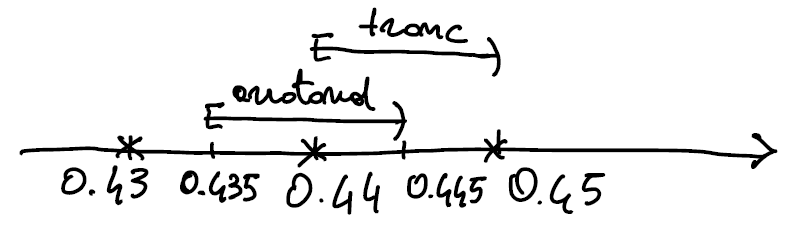
\includegraphics[scale=0.65]{foto/img1}
\end{center}
Vediamo quali numeri sono approssimati da 0,44 per troncamento e per arrotondamento a 2 cifre (notiamo che qui abbiamo numeri del tipo $0,\dotsc$ che quindi coincidono con la propria parte frazionaria).\\
Per \uline{troncamento} 0,44 approssima tutti i numeri dell'intervallo $[0,44 , 0,45)$ che sono del tipo $0,44\dotsc$ (escluso $0,44\overline{999}\dotsc = 0,45$).\\
Invece per \uline{arrotondamento} approssima tutti i numeri dell'intervallo $[0,435 , 0,445)$ \\ 
Infatti approssima per \uline{difetto} tutti i numeri del tipo \[ 0,440\dotsc \] \[ 0,441\dotsc \] \[ 0,442\dotsc \] \[ 0,443\dotsc \] \[ 0,444\dotsc \]
Mentre approssima per \uline{eccesso} tutti i numeri del tipo \[ 0,435\dotsc \] \[ 0,436\dotsc \] \[ 0,437\dotsc \] \[ 0,438\dotsc \] \[ 0,439\dotsc \]
In pratica l'intervallo di troncamento è un intorno destro di $0,44$ di ampiezza $10^{-2}$, mentre l'intervallo di arrotondamento è un intorno simmetrico di raggio $\frac{10^{-2}}{2}$ e ampiezza $10^{-2}$.\\
Risulta evidente dal punto di vista grafico che l'estremo superiore degli errori di troncamento sia $= 10^{-2}$ (entrambi sono intervalli semi aperti a destra) mentre il massimo degli errori di arrotondamento è $\frac{10^{-2}}{2}$ e si ottiene per $x = 0,435$.
\newpage
\section{Lezione 2 - Sistema floating-point}
In questa lezione cominceremo ad occuparci dell'effettivo sistema di rappresentazione dei numeri reali nel calcolatore, ovvero la rappresentazione ``floating-point" (virgola mobile) arrivando a definire l'insieme dei ``reali-macchina" e il concetto chiave di ``precisione di macchina".

\subsection{Sistema floating-point}
Cominciamo con l'osservazione che a partire dalla rappresentazione in base $b$ dei reali vista nella lezione 1, è sempre possibile scrivere $x \in \mathbb{R}$ in base $b$ come 
\[ \begin{split}
    x & = sign(x)( \underbrace{0.d_1 d_2 \dotsc d_t \dotsc}_{\text {\uline{mantissa}}} \cdot {\underbrace{b^p}_{\text{\uline{esponente}}}}) \\
    & = sign(x)\biggl( \sum_{j=1}^\infty d_j b^{-j} \biggr) \cdot b^p
\end{split} \]
$(0,d_1 d_2 \dotsc d_t \dotsc)$ è la ``mantissa" e $d_j\, , 1 \le j < \infty$ le cifre della mantissa, $d_j \in \{0, 1, \dotsc , b-1\}$ e $p \in \mathbb{Z}$ è un intero che viene detto esponente (positivo, nullo o negativo). \\
Si adotta la convenzione che $d_1 \ne 0$, altrimenti ci sarebbero $\infty$ rappresentazioni dello stesso numero.
\begin{esempio}
Base 10
\[ \begin{split}
    1 & = (0.100 \dotsc) \cdot 10^1 \\
    & = (0.0100 \dotsc) \cdot 10^2 \\
    & = (0.00100 \dotsc) \cdot 10^3 \\
    & \dotsc
\end{split}\]
\end{esempio}
In questo modo esiste una sola rappresentazione per ogni numero reale (a meno di periodicità sulla cifra massima ad es. $1 = (0.100 \dotsc) \cdot 10^1$ ma anche $1 = (0.\overline{999} \dotsc) \cdot 10^0$). Questa è quella che si chiama la rappresentazione a ``virgola mobile" (``floating-point" in inglese) del numero. \\
Per capire come funziona basta fare un paio di esempi in base 10.
\begin{esempio}
\[\begin{split}
    x & = + \, 1278.3405 \dotsc \\
    & = + \, (0.12783405 \dotsc) \cdot 10^4 
\end{split}\]
\end{esempio}
Oppure
\begin{esempio}
\[\begin{split}
    x & = - \, 0.0003267 \dotsc \\
    & = - \, (0.3267 \dotsc) \cdot 10^{-3} 
\end{split}\]
\end{esempio}
Come si vede, semplicemente si \uline{sposta la virgola} con un'opportuna potenza della base. \\
Osserviamo che la mantissa sta in $(0,1]$, in particolare $\in [0.1, 1]$ (dove 0.1 è inteso in base $b$, cioè $0.1 = 1 \cdot b^{-1}$ e 1 si ottiene con mantissa periodica sulla cifra massima, ad es. $0.\overline{999} \dotsc = 1$ in base 10). \\
Le cifre della mantissa si chiamano ``cifre significative" del numero. \\
È importante osservare che la mantissa \uline{NON} è la parte frazionaria, chi siano parte intera e parte frazionaria è determinato dall'esponente che sposta la virgola tramite la potenza $b^p$ (a destra per $p>0$ e a sinistra per $p<0$). \\
È chiaro che in generale un reale ha mantissa infinita, in particolare gli irrazionali hanno mantissa infinita in qualsiasi base (perché hanno parte frazionaria infinita). \\
I numeri con \uline{mantissa finita} sono invece \uline{razionali}; che un razionale abbia mantissa finita o meno dipende dalla base, come abbiamo già visto.
\begin{esempio} \end{esempio}
\[\frac{1}{3} = 
\begin{cases}
    (0.100 \dotsc)_3 \cdot 3^0 & \text{base 3} \\
    (0.\overline{333} \dotsc)_{10} \cdot 10^0 & \text{base 10} \\
\end{cases}
\]

\subsection{Insieme dei reali-macchina}
A questo punto siamo in grado di definire l'insieme dei ``reali-macchina", che in un sistema di calcolo con una macchina che lavora in base $b$ sono i numeri con una quantità finita di cifre di mantissa e un esponente che varia in un intervallo finito di interi. \\
Formalmente l'insieme dei reali-macchina è un insieme di razionali definito da 4 parametri: $b$ (la base), $t$ (il numero di cifre della mantissa), $L$ (Lower) e $U$ (Upper) che sono gli estremi dell'intervallo di esponenti interi, dove $L < 0$ e $U > 0$.
\[ \mathbb{F} (b, t, L, U) = \{ \mu \in \mathbb{Q} \colon \mu = sign(\mu)(0.\mu_1 \mu_2 \dotsc \mu_t) \cdot b^p \,, \mu_j \in \{0, 1, \dotsc , b-1\} \,, \mu_1 \ne 0 \,, p \in [L,U] \subset \mathbb{Z} \} \]
$\mathbb{F}$ è l'insieme dei reali-macchina.\\
Il fatto che il numero di cifre di mantissa sia finito e l'intervallo di esponenti sia finito permette la memorizzazione utilizzando sequenza di bit (e tipicamente base $b=2$). \\
Per avere un'idea (poi faremo un modellino) con variabili (zone di memoria) a 64 bit per i reali-macchina (come accade ad es. in Matlab) si ha $b=2$, $t=53$ e in un modello semplificato $L=-\,1023$, $U=+\,1023$. In una parte successiva andremo a studiare più in dettaglio la struttura dell'insieme dei reali-macchina.

\subsection{Stima dell'errore}
Qui invece facciamo il passo fondamentale che ci permette di stimare l'ERRORE che si commette approssimando un numero reale con un reale-macchina. Questa approssimazione avviene per arrotondamento della mantissa al numero di cifre disponibili. \\
Definiamo arrotondamento a $t$ cifre di un numero reale scritto in notazione floating-point \[ x = sign(x)(0.d_1 d_2 \dotsc d_t \dotsc) \cdot b^p \]
il numero \[ fl^t(x) = sign(x)(0.d_1 d_2 \dotsc \Tilde{d}_t) \cdot b^p \]
dove la mantissa è stata arrotondata alla $t$-esima cifra
\[\Tilde{d}_t = 
\begin{cases}
    d_t & \text{se $d_{(t+1)} < \frac{b}{2}$} \\
    d_t+1 & \text{se $d_{(t+1)} \ge \frac{b}{2}$}
\end{cases}
\]
Si tratta a questo punto di stimare l'errore $\lvert \, x - fl^t(x) \, \rvert$.\\
Ora
\[ \begin{split}
    \lvert \, x - fl^t(x) \, \rvert & = \lvert \, (0.d_1 d_2 \dotsc d_t \dotsc) \cdot b^p - (0.d_1 d_2 \dotsc \Tilde{d}_t) \cdot b^p \, \rvert \\
    & = b^p \cdot \lvert (0.d_1 d_2 \dotsc d_t \dotsc) - (0.d_1 d_2 \dotsc \Tilde{d}_t) \rvert
    \end{split}\]
Ma abbiamo già stimato l'errore di arrotondamento a $n$ cifre ``dopo la virgola", che è $\le \frac{b^{-n}}{2}$. Quindi sono in grado di stimare la differenza in modulo tra mantissa esatta e mantissa arrotondata (posto $n = t$)
\[ \lvert \, (0.d_1 d_2 \dotsc d_t \dotsc) - (0.d_1 d_2 \dotsc \Tilde{d}_t) \, \rvert \, \le \, \frac{b^{-t}}{2} \] da cui ricaviamo
\[ \lvert \, x - fl^t(x) \, \rvert \le b^p \cdot \frac{b^{-t}}{2} = \frac{b^{p-t}}{2} \]
Notiamo subito un aspetto: l'errore dipende da $p$, cioè dall'ordine di grandezza del numero (in base $b$).\\
Numeri grandi in modulo ($p$ positivo grande) avranno errori grandi, numeri piccoli in modulo ($p$ negativo e grande in modulo) avranno errori piccoli. \\
Gli errori diventano addirittura grandissimi o piccolissimi avvicinandosi agli estremi $L$ ed $U$ dell'intervallo di esponenti. \\
La domanda è: è accettabile una situazione di questo tipo, ovvero un errore variabile con l'ordine di grandezza del numero, nel modo descritto? \\
La risposta è SI, se ci spostiamo dall'ERRORE ASSOLUTO (che è quello stimato finora) al concetto di ERRORE RELATIVO. \\
Dati due reali $a$ e $\Tilde{a}$, con $\Tilde{a} \approx a$ ($\Tilde{a}$ che approssima $a$) definiamo:
\[ \lvert \, a - \Tilde{a} \, \rvert \quad \longrightarrow \quad \text{ERRORE ASSOLUTO}\]
\[ \frac{\lvert \, a - \Tilde{a} \, \rvert}{\lvert \, a \, \rvert} \, , a \ne 0 \quad \longrightarrow \quad \text{ERRORE RELATIVO} \]
L'errore relativo è l'errore assoluto su una quantità, \uline{pesato dalla grandezza} della quantità. \\
È l'errore più importante in campo sperimentale e nelle applicazioni pratiche, l'errore che di solito si esprime in \uline{percentuale}:
\begin{esempio} \end{esempio}
Una certa quantità è nota con un errore del $10\%$ (errore relativo $10^{-1}$), oppure dell'$1\%$ (errore relativo $10^{-2}$), oppure dello $0.01\%$ (errore relativo $10^{-4}$)
\newline \newline
Nel nostro caso dell'errore di arrotondamento a $t$ cifre di mantissa, scopriremo che l'errore relativo non dipende più da $p$ (cioè dall'ordine di grandezza del numero nella base fissata). Quindi ci interessa ora stimare
\[ \frac{\lvert \, x - fl^t(x) \, \rvert}{\lvert \, x \, \rvert} \quad \text{per}\quad x \ne 0 \]
Abbiamo già stimato il numeratore (che è l'errore assoluto di arrotondamento a $t$ cifre di mantissa), dobbiamo quindi stimare (da sopra) \[ \frac{1}{\lvert \, x  \, \rvert} \]
Per fare questo si stima \uline{da sotto} \[ \lvert \, x \, \rvert \]
infatti, se \[ \lvert \, x \, \rvert \ge \alpha > 0 \] allora 
\[ \frac{1}{\lvert \, x \, \rvert} \le \frac{1}{\alpha} \]
Cerchiamo quindi un tale $\alpha$.
\[ \lvert \, x \, \rvert = (0.d_1 d_2 \dotsc d_t \dotsc ) \cdot b^p \] dove $d_1 \ne 0$. \\
Fissato $p$, qual è il valore più piccolo possibile di $\lvert \, x \, \rvert$? \\
Corrisponde alla mantissa minima che è $0.100 \dotsc = b^{-1}$ quindi
\[ \lvert \, x \, \rvert \ge b^{-1} \cdot b^p = b^{p-1} \] Otteniamo
\[ \frac{\lvert \, x - fl^t(x) \, \rvert}{\lvert \, x \, \rvert} \, \le \, \frac{\cfrac{b^{p-t}}{2}}{b^{p-1}} \,=\, \frac{b^{p-t+1-p}}{2} \,=\, \frac{b^{1-t}}{2} \,=\, \varepsilon_M\]

\subsection{Precisione di macchina}
La quantità $\varepsilon_M$, che si chiama PRECISIONE DI MACCHINA, è il parametro chiave del sistema floating-point, inteso come insieme dei reali-macchina e della sua capacità di approssimazione. \\
In sintesi, possiamo dire che la precisione di macchina è il massimo errore \uline{relativo} di arrotondamento a $t$ cifre di mantissa e dipende solo \uline{da $b$} e \uline{da $t$} o, in altre parole, è la massima distanza relativa dal reale-macchina più vicino, distanza relativa che \uline{non} dipende dall'ordine di grandezza del numero. \\
Come vedremo, non tutti i reali sono approssimabili con un reale-macchina, perché il range di esponenti è finito. Ciononostante, su ogni reale approssimabile si fa un errore che non supera la precisione di macchina. \\
Nel sistema floating-point a 64 bit \[ \varepsilon_M = \frac{2^{1-53}}{2} = 2^{-53}\] 
è una quantità piccolissima ($\approx 10^{-16}$). \\
Osserviamo qui che useremo il simbolo ``$\approx$", che significa ``\textit{circa uguale}", sia nel senso di approssimazione con errore ``piccolo" sia nel senso di approssimazione dell'ordine di grandezza (come l'abbiamo appena usato qui sopra, per indicare che $\varepsilon_M = 2^{-53}$ è dell'ordine di $10^{-16}$). \\
Nella prossima lezione studieremo la struttura dell'insieme $\mathbb{F}(b, t, L, U)$.
\newpage
\section{Lezione 3 - Struttura del sistema floating-point}
In questa lezione studieremo la struttura del sistema floating-point, ovvero dell'insieme dei reali-macchina e dei reali rappresentabili per arrotondamento tramite i reali-macchina.\\
Tratteremo un sistema astratto in base $b$ generica (come fatto finora, con esempi in base 10), per poi discutere un modellino semplificato dello standard a 64 bit (base 2), utilizzato in Matlab e in tutti i principali linguaggi di calcolo.

\subsection{Proprietà del sistema}
Ricordiamo che i reali-macchina in base $b$ a $t$ cifre di mantissa e con range di esponenti $[L,U] \subset \mathbb{Z}$ sono definiti da
\[ \mathbb{F}(b, t, L, U) = \{ \mu \in \mathbb{Q} : \mu = sign(\mu)\cdot (0,\mu_1 \mu_2 \dotsc \mu_t) \cdot b^p \,,\, \mu_j \in \{ 0, 1, \dotsc, b-1 \} \,,\, \mu_1 \ne 0 \,,\, p \in [L,U] \subset \mathbb{Z} \} \]
dove $\mu_j$, $j = 1, \dotsc, t$ sono le cifre della mantissa e $p$ l'esponente intero della potenza della base che sposta la virgola dove $L<0$ e $U>0$, quindi $p$ appartiene all'intervallo di interi $L, L+1, \dotsc, -1, 0, 1, \dotsc, U-1, U$.\\
Risponderemo ad alcune domande di base:
\begin{itemize}
    \item quanti sono i reali-macchina?
    \item quali reali sono approssimabili per arrotondamento con i reali-macchina?
    \item come sono distribuiti sull'asse reale i reali-macchina?
\end{itemize}
In modo molto schematico, sintetizziamo con un disegno 
\begin{center}
    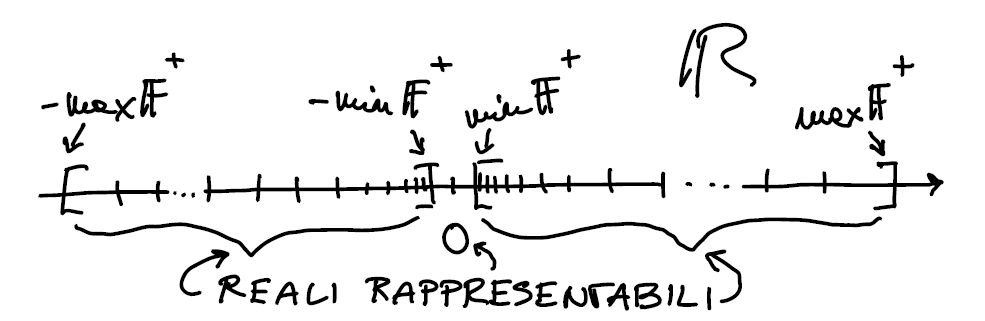
\includegraphics[scale=0.65]{foto/img2}
\end{center}
In questo schemino grafico i reali-macchina corrispondono all'insieme \uline{finito} di tacche sull'asse reale e a parte lo 0 che è un reale-macchina (con una rappresentazione speciale visto che la mantissa nulla non è ammessa) \uline{stanno nell'unione di due intervalli simmetrici}. Infatti, detti $\mathbb{F}^+$ i reali-macchina $>0$ e $\mathbb{F}^-$ quelli $<0$, abbiamo che $\mathbb{F}^- = - \mathbb{F}^+$ (cioè si cambia segno a tutti i positivi, $\mathbb{F}^+$ e $\mathbb{F}^-$ sono simmetrici rispetto a 0) 
\[ \mathbb{F}^+ \subset [\,\min \mathbb{F}^+, \max \mathbb{F}^+\,] \]
\[ \mathbb{F}^- \subset [\,- \max \mathbb{F}^+, - \min \mathbb{F}^+\,] \]
Questi \uline{due intervalli} nel continuo sono proprio i \uline{reali approssimabili} tramite i reali-macchina per arrotondamento a $t$ cifre della mantissa, con un errore relativo $\le \varepsilon_M = \frac{b^{1-t}}{2}$ (la precisione di macchina). Invece i reali che in modulo sono $> \max \mathbb{f}^+$ e quelli che in modulo solo $< \min \mathbb{f}^+$, sono ``troppo grandi" o ``troppo piccoli" per essere approssimati e costituiscono quello che si chiama l'OVERFLOW e l'UNDERFLOW nel sistema floating-point.\begin{center}
    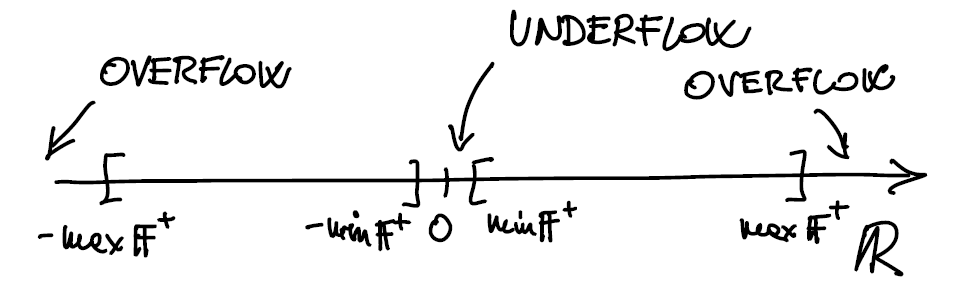
\includegraphics[scale=0.65]{foto/img3}
\end{center}
L'UNDERFLOW è un intorno di 0, l'OVERFLOW un intorno di $\infty$.\\
Il problema è che l'esponente $p$ di tali numeri è fuori dal range di esponenti ammissibili, ovvero $[L,U] \subset \mathbb{Z}$ (cioè $p < L$ (underflow) oppure $p > U$ (overflow)).\\
La comparsa di numeri in overflow/underflow durante un processo di calcolo altera il processo stesso facendogli tendenzialmente perdere di significato. \\
Nei vecchi linguaggi di programmazione (ad esempio il Fortran) la comparsa di overflow determinava addirittura l'arresto del processo di calcolo con un messaggio di errore. In Matlab invece (e in altri linguaggi) un numero in overflow, generato ad esempio dal prodotto di reali-macchina molto grandi in modulo, viene indicato con simbolo ``\texttt{Inf}" (infinito) ed entra nel processo di calcolo alterandolo, generando altri ``\texttt{Inf}" o forme indeterminate (ad es.$\frac{\texttt{Inf}}{\texttt{Inf}}$) che vengono indicate col simbolo ``\texttt{NaN}" (Not a Number).\\
Per questo negli algoritmi numerici è importante cercare di prevenire overflow/underflow. \\
A questo punto conviene calcolare $\min \mathbb{F}^+$ e $\max \mathbb{F}^+$, modo da quantificare gli estremi degli intervalli di rappresentazione visto che un reale-macchina ha la struttura 
\[\mu = \text{segno} \cdot \text{mantissa} \cdot b^p\]
Il minimo positivo si otterrà moltiplicando la minima mantissa per la potenza della base con il minimo esponente
\[ \text{\uline{mantissa minima}} = (0,10 \dotsc 0)_b = 1 \cdot b^{-1}\]
\[ \text{\uline{esponente minimo}} = L\]
quindi
\begin{table}[h!]
    \centering
    \begin{tabular}{|c|}
    \hline
        $\min \mathbb{F}^+ = b^{L-1}$ \\
    \hline
    \end{tabular}
\end{table}
Invece il massimo positivo si otterrà moltiplicando la mantissa massima per la potenza della base col massimo esponente
\[ \text{\uline{mantissa massima}} = (0,\underbrace{b-1} \underbrace{b-1} \dotsc \underbrace{b-1})_b\]
cioè tutte le $t$ cifre sono uguali alla cifra massima che è $b-1$
\begin{esempio}
$(0,99 \dotsc 9)_{10}$ in base 10
\end{esempio}
Calcoliamo usando la somma geometrica di ragione $b^{-1}$
\[\begin{split}
    \text{\uline{mantissa max}} & = \sum_{j=1}^t\,(b-1)\,b^{-1} \\
    & = (b-1)\,\sum_{j=1}^t\,b^{-1} \\
    & = (b-1)\,\biggl(\sum_{j=0}^t\,b^{-1} - 1\biggr) \\
    & = (b-1)\,\biggl(\frac{1 - b^{-(t+1)}}{1 - \frac{1}{b}} - 1\biggr) \\
    & = (b-1)\,\biggl(\frac{b - b^{-t}}{b - 1} - 1\biggr) \\
    & = 1 - b^{-t} \\
\end{split}\]
Ora \[ \text{\uline{esponente massimo}} = U\] quindi
\begin{table}[h!]
    \centering
    \begin{tabular}{|c|}
    \hline
        $\max \mathbb{F}^+ = (1 - b^{-t})\,b^U$ \\
    \hline
    \end{tabular}
\end{table}
\begin{esempio} 
In base 10 con 16 cifre di mantissa ed esponenti minimo $L = - 307$ e massimo $U = + 308$ (modello che come vedremo corrisponde in sostanza all'interfaccia del Matlab, ben sapendo però che la base interna del calcolatore è 2 e non 10)
\[ \min \mathbb{F}^+ = 10^{- 1 - 307} = 10^{- 308} \]
\[ \max \mathbb{F}^+ = (1 - 10^{-16})\cdot 10^{308} \approx 10^{308}\]
\end{esempio}
I reali rappresentabili tramite reali-macchina in Matlab sono quindi intervalli estremamente ampi, con un estremo ``grandissimo" e un estremo ``piccolissimo" (in modulo, considerando anche l'intervallo dei negativi). \\
È importante però ricordare ancora una volta che la rappresentazione avviene per arrotondamento della mantissa e che gli \uline{unici} numeri effettivamente memorizzabili nel calcolatore sono i \uline{reali-macchina}, un \uline{insieme finito}.\\
Ma qual è la \uline{cardinalità} (numero di elementi) di $\mathbb{F}$? Il calcolo è facile, osservando che basta contare gli elementi di $\mathbb{F}^+$ e raddoppiare, tenendo poi conto dello 0 che ha una rappresentazione speciale
\[\begin{split}
    \text{card}(\mathbb{F}^+) & = \text{numero possibili mantisse} \,\cdot\, \text{numero possibili esponenti} \\
    & = (b-1)\cdot \underbrace{b \cdot \dotsc \cdot b}_{t - 1 \,\text{fattori}} \cdot \, (U - L + 1) \\
    & = (b-1)\cdot b^{t - 1} \cdot \, (U - L + 1) \\
\end{split}\]
In questo conto si osservi che per la prima cifra di mantissa ci sono $b - 1$ scelte (non può essere 0), mentre ci sono $b$ scelte per tutte le altre cifre (ad es. in base 10 la prima cifra può essere $1, 2, \dotsc , 9$ cioè 10 possibili cifre). \\
Il numero di elementi dell'intervallo di interi $[L,U]$ è $U-L+1$. Alla fine si ottiene
\[ \text{card}(\mathbb{F}) = 1 + 2 \cdot (b-1)\cdot b^{t - 1} \cdot \, (U - L + 1) \]
Nel modello simil-Matlab visto prima con $b = 10$, $t = 16$, $L = -307$, $U = +308$ si ottiene \[ \text{card}(\mathbb{F}) = 1 + 2 \cdot 9\cdot 10^{15} \cdot \, 616 \]
che è un numero dell'ordine di $10^{19}$.\\
Da dove vengono i parametri che abbiamo usato per il modello simil-Matlab? Dal fatto che il Matlab usa uno standard di rappresentazione per i reali-macchina (lo standard IEEE) in cui ad una variabile reale è dedicata una sequenza di 64 bit (8 byte), in cui 1 bit è riservato al segno, 52 bit alla mantissa e 11 bit all'esponente. \\
Senza entrare in dettaglio nello standard di rappresentazione facciamo un semplice modello:
\begin{center}
    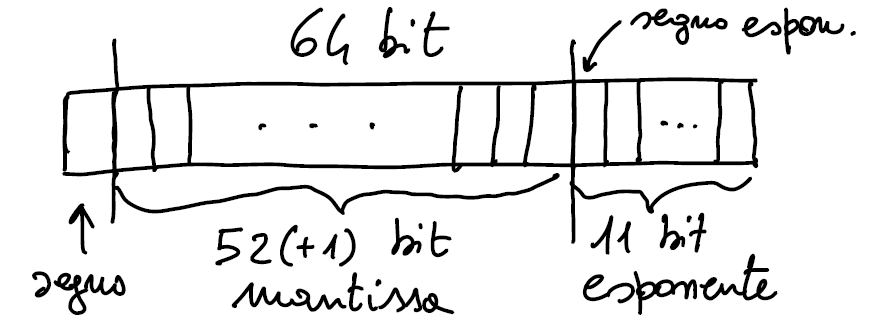
\includegraphics[scale=0.65]{foto/img4}
\end{center}
In ciascuna delle caselline (bit) si può scrivere 0 oppure 1 (per il segno uno dei due rappresenta ``+" e l'altro ``-"). Per quanto riguarda la mantissa i bit sono 52 ma è come se fossero 53, perché la prima cifra di mantissa deve essere non nulla e quindi per forza 1 (ovvero il processore tratta i numeri come se avessero mantissa $0,1 d_2 \dotsc d_{53}$ con $d_j \in \{0,1\},\, 2 \le j \le 53$) quindi la \uline{precisione di macchina} è
\[ \varepsilon_M = \frac{2^{1-53}}{2} = 2^{-53} \approx 10^{-16}\]
Per quanto riguarda il range di esponenti, in questo modello semplificato degli 11 bit a disposizione ne teniamo uno per il segno. Quindi $\max \, \lvert \, p \, \rvert$ si ottiene con la sequenza
\[ (\underbrace{11\dotsc1}_{\text{10 cifre}})_2 \]
ovvero
\[ \max \, \lvert \, p \, \rvert = \sum_{j=0}^9 2^j = \frac{2^{10} - 1}{2 - 1} = 1023 \]
Ricordando le proprietà della somma geometrica (qui con ragione 2) viste nella lezione 1, allora \[ U = +1023 \,,\, L = -1023 \] e
\[ \max \, \mathbb{F}^+ \, \approx 2^{1023} \approx 10^{308}\]
\[ \min \, \mathbb{F}^+ \, = 2^{-1024} \approx 10^{-308}\]
(in realtà la codifica dell'esponente usa una tecnica un po' più sofisticata ma la sostanza cambia poco) \\
Alla fine possiamo dire che in Matlab (e molti altri linguaggi) i reali-macchina sono sequenze a 64 bit (la cosiddetta precisione doppia) corrispondenti sostanzialmente a
\[ \mathbb{F}(2, 53, -1023, +1023) \]
Siccome l'interfaccia dei linguaggi con l'utente è in base 10 (con conversione automatica dell'input/output) per quanto visto sopra possiamo dire che lavorando in Matlab è essenzialmente (ma non esattamente) come se utilizzassimo
\[ \mathbb{F}(10, 16, -307, +308) \]
nel senso che l'ordine di grandezza dei parametri chiave $\varepsilon_M, \max \mathbb{F}^+, \min \mathbb{F}^+$ è corretto (ma scopriremo che talvolta bisogna tener presente che la base ``vera" è 2). \\
Finora abbiamo risposto a due delle tre domande iniziali sulla struttura del sistema floating-point, resta da analizzare come sono distribuiti i reali-macchina.

\subsection{Distribuzione dei reali-macchina}
Il concetto chiave è che \uline{non} sono distribuiti \uline{uniformemente}, ma bensì ``\uline{a densità variabile}", i reali-macchina ``piccoli" sono vicini, i reali-macchina ``grandi" sono distanti tra di loro, la densità cresce andando verso $\pm \min \mathbb{F}^+$ e decresce andando verso $\pm \max \mathbb{F}^+$. \\
Questo si può capire bene calcolando la distanza tra reali-macchina consecutivi (con lo stesso esponente $p$).\\
Graficamente (ad es. in $\mathbb{F}^+$) 
\begin{center}
    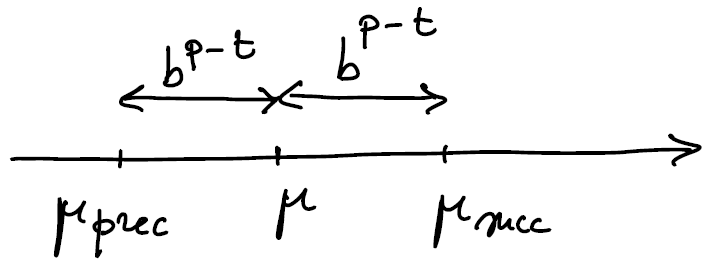
\includegraphics[scale=0.65]{foto/img5}
\end{center}
Infatti due reali-macchina consecutivi differiscono di 1 nella $t$-esima cifra di mantissa, ovvero
\[ \text{mantissa}(\mu_{\text{succ}})\,-\,\text{mantissa}(\mu) = 1 \cdot b^{-t}\] e 
\[ \mu_{\text{succ}}\,-\,\mu = b^{-t} \cdot b^p = b^{p-t} \]
La distanza (assoluta) è quindi variabile con $p$, cioè con l'ordine di grandezza del numero in base $b$. \\
Questa distanza varia (di un fattore $b$) quando si passa per una potenza della base.
\begin{esempio}
$b = 10$ e $t = 2$ (due cifre di mantissa) 
\begin{center}
    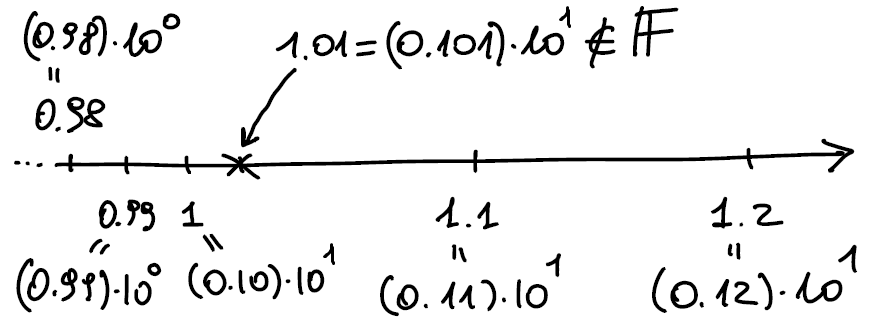
\includegraphics[scale=0.65]{foto/img6}
\end{center}
\end{esempio}
La domanda è: chi è il reale-macchina successivo ad 1? Pensando a 2 cifre decimali, verrebbe da rispondere 1,01 ma \uline{non} è così, perché $1,01 = (0,101)\cdot 10^1$ ha 3 cifre di mantissa e in questo esempio $t=2$.\\
Invece il reale-macchina successivo ad 1 è $(0,11)\cdot 10^1 = 1,1$ passando per $1 = 10^0$ la distanza è cresciuta di un fattore 10, da $10^{-2}$ a $10^{-1}$.\\
Pensando invece a quali reali sono approssimati da 0,99, 1 e 1,1 abbiamo graficamente
\begin{center}
    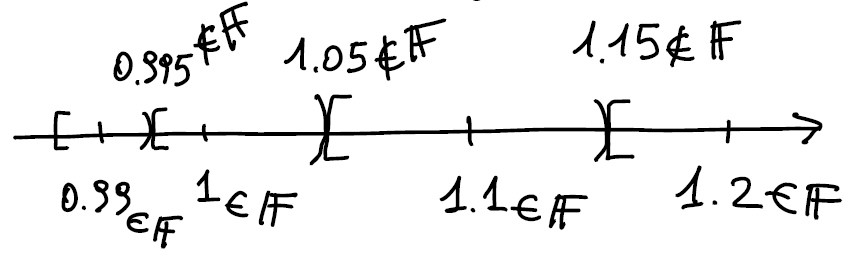
\includegraphics[scale=0.65]{foto/img7}
\end{center}
Vediamo che ogni reale-macchina è il centro di un intorno di approssimazione a $t$ cifre di mantissa (qui $t=2$): questi intorni sono generalmente simmetrici e di raggio $\frac{b^{p-t}}{2}$ \begin{center}
    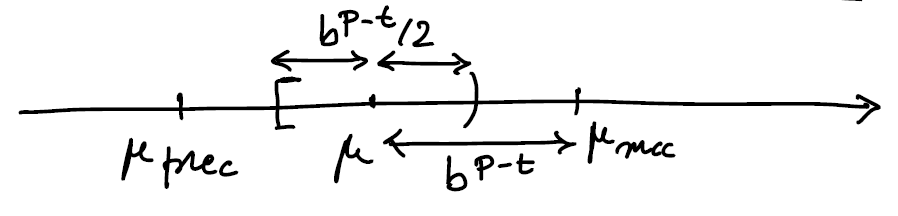
\includegraphics[scale=0.65]{foto/img8}
\end{center}
tranne per $\mu = b^k$, nel qual caso l'intorno è asimmetrico e l'intorno destro (in $\mathbb{F}^+$) si allunga di un fattore $b$.\\
Tutti i reali di questi intorni vengono approssimati dal reale-macchina centro dell'intorno per arrotondamento a $t$ cifre di mantissa, con un errore assoluto $\le \frac{b^{p-t}}{2} =$ raggio. Ma se andiamo a stimare l'\uline{errore relativo}, sappiamo dalla lezione 2 che questo non può superare la precisione di macchina \[ \varepsilon_M = \frac{b^{1-t}}{2} \]
che è \uline{indipendente da $p$}.\\
L'unione di tutti gli intorni di approssimazione per arrotondamento copre gli intervalli dei reali rappresentabili, ovvero
\[ [- \max \mathbb{F}^+ , - \min \mathbb{F}^+] \cup [\min \mathbb{F}^+ , \max \mathbb{F}^+]\]
Come descritto in modo un po' ingenuo da questo disegno (per $\mathbb{F}^+$) 
\begin{center}
    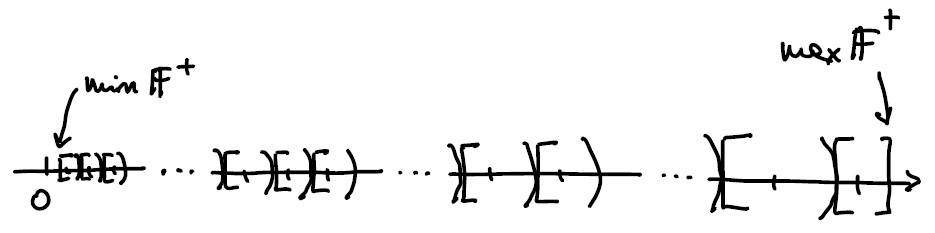
\includegraphics[scale=0.65]{foto/img9}
\end{center}
Concludiamo questa lezione con due esempi semplici in base 10:
\begin{esempio} \end{esempio}
Disegnare $\mathbb{F}(10, 1, -1, 1)$ \\
Abbiamo una sola cifra di mantissa (il minimo possibile) ed esponenti $p = -1, 0, 1$.\\
Disegniamo $\mathbb{F}^+$ (scrivendo per semplicità i reali-macchina in notazione standard) 
\begin{center}
    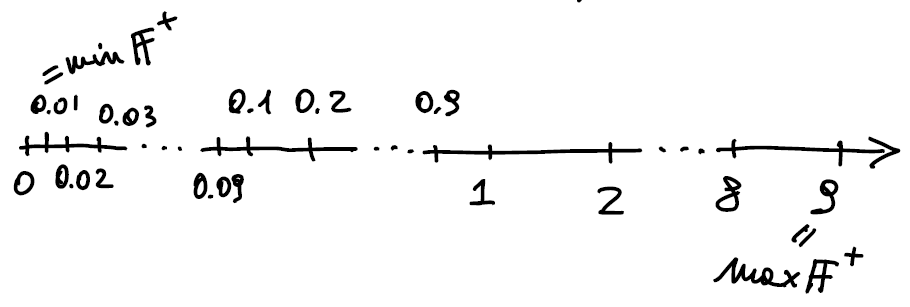
\includegraphics[scale=0.65]{foto/img10}
\end{center}
Vediamo che si parte dall'ordine di grandezza dei centesimi con 
\[ \min \mathbb{F}^+ = 0,1 \cdot 10^{-1} = 0,01 \]
(tra i centesimi non ci sono reali-macchina perché c'è una sola cifra di mantissa), si passa ai decimi, poi alle unità sempre senza reali-macchina intermedi, fino a
\[ \max \mathbb{F}^+ = 0,9 \cdot 10^1 = 9 \]
La precisione di macchina è 
\[ \varepsilon_M = \frac{10^{1-t}}{2} = \frac{10^{1-1}}{2} = \frac{1}{2} = 50\% \]
Si tratta di un sistema floating-point molto ``povero", perché c'è una sola cifra di mantissa e un'estensione molto limitata dal piccolo range di esponenti.

\begin{esempio} \end{esempio}
Disegnare $\mathbb{F}(10, 2, -2, 2)$ \textbf{PER ESERCIZIO} (converrà fare degli opportuni ``zoom" sui vari ordini di grandezza). Il sistema è più ``ricco" del precedente, infatti abbiamo
\[ \min \mathbb{F}^+ = b^{L-1} = 10^{-3} \]
\[\begin{split}
    \max \mathbb{F}^+ & = (1 - b^{-t}) \cdot b^U \\
    & = (1 - 10^{-2}) \cdot 10^2 = 99
\end{split}\]
\[ \varepsilon_M = \frac{b^{1-t}}{2} = \frac{10^{-1}}{2} = 5\% \]
Si parte dai millesimi, ma fra questi ci sono i decimillesimi perché abbiamo 2 cifre di mantissa, poi ai centesimi con i millesimi, i decimi con i centesimi, le unità con i decimi e infine le decine con le unità.
\newline \newline
Questo dovrebbe far capire quanto ricca è la struttura del sistema floating-point a 64 bit (\uline{precisione doppia}). \\
È il caso di ricordare che esistono altri standard, la precisione \uline{singola} (a 32 bit) con $\varepsilon_M \approx 10^{-8}$ e la precisione \uline{quadrupla} (a 128 bit) con $\varepsilon_M \approx 10^{-32}$.\\
Quale sia la precisione di default dipende dal linguaggio, alcuni permettono di scegliere tra singola, doppia e quadrupla. \\
Queste precisioni corrispondono ad operazioni aritmetiche implementate a livello hardware (circuiti) nel processore, quindi estremamente veloci. \\
In alcuni linguaggi è possibile aumentare la precisione (cioè aumentare il numero di cifre di mantissa), ma allora le operazioni aritmetiche sono implementate a livello software (c'è un programma che calcola somma, moltiplicazione e divisione, non un'unità hardware), quindi il costo delle operazioni cresce e cresce ovviamente l'occupazione di memoria, soprattutto elaborando masse di dati. \\
Questo è il motivo per cui si è fatto un compromesso e lo standard attuale è la precisione doppia con $\varepsilon_M = 2^{-53} \approx 10^{-16}$, un massimo errore relativo di arrotondamento che è di solito molto più piccolo degli errori di misura sperimentale dei dati nelle applicazioni.\\
Ciononostante, vedremo che la propagazione degli errori in algoritmi instabili può far perdere anche tutta questa precisione nel processo di calcolo. \\
Questo conduce in modo naturale allo studio della STABILITÀ degli algoritmi numerici, che cominceremo già nella prossima lezione sulle operazioni aritmetiche con numeri approssimati.
\newpage
\section{Lezione 4 - Operazioni aritmetiche con numeri approssimati}
Nelle lezioni precedenti abbiamo discusso una delle basi del calcolo numerico: il sistema floating-point di rappresentazione dei numeri reali nel calcolatore. \\
Il concetto cardine è quello di precisione di macchina, il massimo errore relativo di arrotondamento di un numero reale rappresentabile (ovvero non in overflow o underflow) con il reale-macchina ``più vicino".\\
In questa lezione inizieremo ad entrare nel cuore del calcolo numerico, trattando innanzitutto le operazioni aritmetiche nel sistema floating-point, cioè quale sia l'effetto degli errori sui dati, sul risultato dell'operazione.\\
L'analisi che faremo sarà però più generale e permetterà di studiare la risposta agli errori sui dati delle operazioni aritmetiche qualunque sia la fonte di errore (ad esempio errori di misura sperimentale).

\subsection{Operazione macchina}
Cominciamo col definire il concetto di OPERAZIONE-MACCHINA.\\
Sia $\bigstar$ un'operazione aritmetica sui reali, ovvero \[ \bigstar =
\begin{cases}
    \pm & \text{addizione, sottrazione} \\
    * & \text{moltiplicazione} \\
    / & \text{divisione}
\end{cases}
\]
Allora, dato un insieme di reali-macchina $\mathbb{F}(b, t, L, U)$ il modo in cui il processore realizza l'operazione tra due reali rappresentabili $x, y$ è 
\begin{center}
    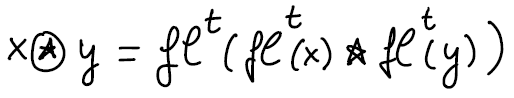
\includegraphics[scale=0.65]{foto/img11}
\end{center}
ovvero il modello è il seguente:
\begin{enumerate}
    \item i due reali vengono arrotondati
    \item viene fatta l'operazione tra gli arrotondamenti
    \item il risultato viene a sua volta arrotondato
\end{enumerate}
È importante osservare da subito che le operazioni-macchina nel sistema floating-point perdono varie proprietà delle operazioni aritmetiche teoriche. Ad esempio, mentre la proprietà commutativa di addizione e moltiplicazione resta valida, in generale non sono più valide la proprietà associativa e distributiva.\\
Facciamo un esempio in cui non vale la proprietà associativa della moltiplicazione,per problemi di overflow.
\begin{esempio} \end{esempio}
Consideriamo $\mathbb{F} = (10, 16, -307, 308)$ che come abbiamo visto corrisponde sostanzialmente all'interfaccia del Matlab. Siano
\[ a = 10^{200}\,,\,b = 10^{150}\,,\,c = 10^{-50} \]
in aritmetica reale \[ (a \times b) \times c = a \times (b \times c) = 10^{300} \]
Ma con le limitazioni date per gli esponenti \[(a \otimes b) \otimes c = \text{overflow}\]
perché  \[a \otimes b = 10^{350} \quad \text{e} \quad 350 >308\]
invece \[ a \otimes (b \otimes c) = 10^{200} \otimes 10^{100} = 10^{300} \]
Quindi \[ (a \otimes b) \otimes c \underbrace{\ne}_{\text{NO ASSOCIATIVA}} a \otimes (b \otimes c) = a \times b \times c \]
\newline \newline
Come vedremo più avanti, la proprietà associativa (e anche la distributiva) possono saltare anche per effetto degli errori di arrotondamento.\\
D'altra parte, c'è un'altra proprietà che non è più valida a causa dell'arrotondamento, l'unicità dell'elemento neutro dell'addizione.\\
Per capirlo, consideriamo di nuovo un sistema floating-point “virtuale” $\mathbb{F} = (10, 16, -307, 308)$ (qui in realtà conta essenzialmente il numero di cifre mantissa). Si ha 
\[ 1 \oplus 10^{-16} = 1\]
cioè $10^{-16}$ si comporta come 0 nell'addizione con 1, mentre 
\[ 1 \oplus 10^{-15} = 1 + 10^{-15}\]
Perché? Basta riflettere sul fatto che le cifre di mantissa sono 16, ma17cifra
\[ 1 + 10^{-16} = (0,100 \dotsc 0 \underbrace{1}_{17^\circ\text{ cifra}}) \cdot 10^1\]
viene arrotondato ad 1 perché la prima cifra trascurata è \[ 1 < \frac{b}{2} = 5 \]
Invece \[ 1 + 10^{-15} = (0,100 \dotsc 0 \underbrace{1}_{16^\circ\text{ cifra}}) \cdot 10^1\] 
e non c'è bisogno di alcun arrotondamento.
D'altra parte, si vede anche subito che $ 10^{-1} \oplus 10^{-16} = 10^{-1} + 10^{-16} $ cioè $10^{-16}$ non è l'elemento neutro per $10^{-1}$.\\
In questo contesto si può dare una seconda caratterizzazione della precisione di macchina (che non dimostriamo)
\[ \varepsilon_M = \min \{\mu \in \mathbb{F}^+ : 1 \oplus \mu > 1\} \]

\subsection{Risposta delle operazioni agli errori sui dati}
Passiamo alla questione chiave: la risposta delle operazioni agli errori \uline{sui dati}.\\
Possiamo osservare fin da subito che l'arrotondamento finale del risultato ha un errore che non può superare la precisione di macchina \[ \varepsilon_M = \frac{b^{1-t}}{2}\]
e quindi è ininfluente ai fini dell'analisi dell'effetto degli errori sui dati. \\
Invece l'errore chiave da stimare è l'errore \uline{relativo} 
\[ \varepsilon_{x \star y} = \frac{\lvert (x \star y) - (fl^t (x) \star fl^t (y)) \rvert}{\lvert (x \star y) \rvert} \]
(purché $(x \star y) \ne 0$) in funzione degli errori relativi sui dati
\[ \varepsilon_x = \frac{\lvert x - \Tilde{x} \rvert}{\lvert x \rvert}, \quad x \ne 0 \]
\[ \varepsilon_y = \frac{\lvert y - \Tilde{y} \rvert}{\lvert y \rvert}, \quad y \ne 0 \]
Più in generale, dati due numeri reali $x, y \ne 0$ e due loro approssimazioni $\Tilde{x} \approx x\,,\, \Tilde{y} \approx y$ (dove supponiamo di conoscere o meglio di saper stimare gli errori relativi $ \varepsilon_x = \frac{\lvert x - \Tilde{x} \rvert}{\lvert x \rvert}$ e $ \varepsilon_y = \frac{\lvert y - \Tilde{y} \rvert}{\lvert y \rvert}$ ) andremo a stimare l'errore relativo sul risultato dell'operazione $\star$, commesso utilizzando i dati approssimati invece dei dati esatti, cioè
\[ \varepsilon_{x \star y} = \frac{\lvert (x \star y) - (\Tilde{x} \star \Tilde{y}) \rvert}{\lvert (x \star y) \rvert}, \quad x \star y \ne 0 \]
in funzione di $\varepsilon_x$, $\varepsilon_y$ (nel caso delle operazioni-macchina si ha $\Tilde{x} = fl^t(x)$, $\Tilde{y} = fl^t(y)$, $\varepsilon_x$, $\varepsilon_y \le \varepsilon_M$).
Diremo STABILE un'operazione aritmetica per cui l'errore sul risultato ha lo stesso ordine di grandezza dell'errore (massimo) sui dati.

\subsubsection{Moltiplicazione}
Iniziamo con la MOLTIPLICAZIONE (indicheremo il prodotto con la notazione standard $\times \, y$, sapendo che nei linguaggi di calcolo il simbolo delle moltiplicazione è *).
\[ \varepsilon_{xy} = \frac{\lvert \, xy - \Tilde{x}\Tilde{y} \, \rvert}{\lvert \, xy \, \rvert}, \quad x , y \ne 0 \]
Usiamo la stessa tecnica che si usa per dimostrare che il limite del prodotto di due successioni o funzioni è il prodotto dei limiti, aggiungendo e togliendo a numeratore ad esempio $\Tilde{x}y$
\[\begin{split}
    \varepsilon_{xy} & = \frac{\lvert \, xy - \Tilde{x}y + \Tilde{x}y - \Tilde{x}\Tilde{y} \, \rvert}{\lvert \, y \, \rvert} \\
    & = \frac{\lvert \, \overbrace{y(x - \Tilde{x})}^{=\,a} + \overbrace{x(y - \Tilde{y})}^{=\,b} \, \rvert}{\lvert\, xy \, \rvert} \\
    & \le \frac{\lvert \, y(x - \Tilde{x}) + x(y - \Tilde{y}) \, \rvert}{\lvert \, xy \, \rvert} \quad \quad (\bigstar) 
\end{split}\]
dove abbiamo utilizzato la DISUGUAGLIANZA TRIANGOLARE che è uno strumento chiave per fare stime.\\
Dati $a, b \in \mathbb{R}$
\[ \lvert \lvert \, a \, \rvert - \lvert \, b \, \rvert \rvert \le \lvert \, a + b \, \rvert \le \lvert \, a \, \rvert + \lvert \, b \, \rvert\] 
Quindi da $(\bigstar)$ otteniamo (ricordando che il modulo del prodotto è il prodotto dei moduli)
\[ \varepsilon_{xy} \le \frac{\lvert \,y\, \rvert \lvert \,x - \Tilde{x}\, \rvert}{\lvert \,xy\, \rvert} + \frac{\lvert \,\Tilde{x}\, \rvert \lvert \,y - \Tilde{y}\, \rvert}{\lvert \,xy\, \rvert} = \varepsilon_x + \frac{\lvert \,\Tilde{x}\, \rvert}{\lvert \,x\, \rvert} \varepsilon_y\]
Questo perché $\frac{\lvert \,x - \Tilde{x}\, \rvert}{\lvert \,x\, \rvert} = \varepsilon_x$ e $\frac{\lvert \,y - \Tilde{y}\, \rvert}{\lvert \,y\, \rvert} = \varepsilon_y$.\\
Ora, siccome $\Tilde{x} \approx x$, possiamo dire almeno qualitativamente che $\frac{\lvert \,\Tilde{x}\, \rvert}{\lvert \,x\, \rvert} \approx 1$ e quindi 
\[ \varepsilon_{xy} \le \varepsilon_x + \frac{\lvert \,\Tilde{x}\, \rvert}{\lvert \,x\, \rvert} \varepsilon_y \approx \varepsilon_x + \varepsilon_y \]
cioè che l'operazione di moltiplicazione è STABILE (l'errore relativo sul risultato è maggiorato da una quantità che è dell'ordine dell'errore sui dati).\\
Per esprimere questo fatto possiamo usare la notazione \[\varepsilon_{xy} \lesssim \varepsilon_x + \varepsilon_y \]
dove $\lesssim$ non è una disuguaglianza esatta ma va intesa nel senso indicato sopra. \\
In realtà, possiamo dare anche una \uline{stima} quantitativa osservando che per la disuguaglianza triangolare 
\[ \frac{\lvert \,\Tilde{x}\, \rvert}{\lvert \,x\, \rvert} = \frac{\lvert \, \overbrace{x}^{=\,a} + \overbrace{\Tilde{x} - x}^{=\,b} \, \rvert}{\lvert\, x \, \rvert} \le \frac{\lvert \, x \, \rvert + \lvert \,\Tilde{x} - x\, \rvert}{\lvert\, x \, \rvert} = 1 + \varepsilon_x\]
e quindi \[ \varepsilon_{xy} \le \varepsilon_x + (1 + \varepsilon_x)\,\varepsilon_y\]
Nel caso della moltiplicazione-macchina in precisione doppia $\varepsilon_x \le \varepsilon_M \approx 10^{-16}$ e quindi $1 + \varepsilon_x$ è vicinissimo ad 1.\\
Ma anche con $\varepsilon_x \approx 10^{-1}$ (ad esempio un errore di misura del $10\%$, che è un errore sperimentale grande) avremmo $1 + \varepsilon_x \approx 1,1$ e quindi la sostanza della stabilità non cambia.

\subsubsection{Divisione}
Passiamo ora alla DIVISIONE: siccome la divisione $\frac{x}{y}, \, y \ne 0$ è la moltiplicazione per il reciproco, $\frac{x}{y} = x \cdot \frac{1}{y}$, ci basta analizzare la stabilità dell'operazione di reciproco
\[ \varepsilon_{\frac{1}{y}} = \frac{\abs*{\,\frac{1}{y} - \frac{1}{\Tilde{y}}\,} }{\abs*{\,\frac{1}{y}\,}} = \frac{\frac{\abs*{\,\Tilde{y} - y\,}}{\abs*{\,\Tilde{y}y\,}}}{\abs*{\,\frac{1}{y}\,}} = \frac{\abs*{\,\Tilde{y} - y\,}}{\abs*{\,y\,}} \cdot \frac{\abs*{\,y\,}}{\abs*{\,\Tilde{y}\,}} \approx \varepsilon_y \qquad \Bigl( \text{questo perché } \frac{\abs*{\,\Tilde{y} - y\,}}{\abs*{\,y\,}} = \varepsilon_y . \Bigr)\]
con l'ipotesi qualitativa che $\abs{y} \approx \abs{\Tilde{y}}$ e quindi $\frac{\abs*{\,y\,}}{\abs*{\,\Tilde{y}\,}} \approx 1$ ne deduciamo che anche che la DIVISIONE è un'operazione STABILE, perché il reciproco è stabile e la moltiplicazione è stabile.\\
Anche in questo caso possiamo però quantificare, stimando meglio $\frac{\abs*{\,y\,}}{\abs*{\,\Tilde{y}\,}}$.\\ 
Assumiamo $\varepsilon_y = \frac{\abs*{\,y - \Tilde{y}\,}}{\abs*{\,y\,}} < 1$ (cioè che l'errore relativo sia minore di 1, il che vuol dire $< 100\%$, che sarà vero in tutte le situazioni “ragionevoli”, visto che tipicamente l'errore sarà molto più piccolo di 1), allora 
\[ \abs{\,\Tilde{y}\,} = \abs{\,y + \Tilde{y} - y\,} = \abs{y}\abs*{\,1 + \frac{(\Tilde{y} - y)}{y}\,}\]
usando la stima da sotto nella disuguaglianza triangolare 
\[\abs{\, a + b\,} \ge \abs{\,\abs{\,a\,} - \abs{\,b\,}\,}\]
$a = 1$ e $b = \frac{(\Tilde{y} - y)}{y}$
\[\abs*{\,1 + \frac{(\Tilde{y} - y)}{y}\,} \ge \abs*{\,1 - \frac{\abs*{\,\Tilde{y} - y\,}}{\abs{\,y\,}}\,} = \abs*{\,1 - \varepsilon_y\,} = 1 - \varepsilon_y \qquad \Bigl( \text{perché } \varepsilon_y < 1 \Bigr)\]
da cui si ottiene 
\[\abs{\,\Tilde{y}\,} \ge \abs{\,y\,}(1 - \varepsilon_y)\]
e quindi
\[\frac{\abs*{\,y\,}}{\abs*{\,\Tilde{y}\,}} \le \frac{\abs*{\,y\,}}{\abs{\,y\,}(1 - \varepsilon_y)} = \frac{1 + \varepsilon_y}{(1 + \varepsilon_y)(1 - \varepsilon_y)} = \frac{1 + \varepsilon_y}{1 - \varepsilon_y^2} \approx 1 + \varepsilon_y\]
perché $\varepsilon_y^2 \ll \varepsilon_y < 1$ (per la prima volta usiamo qui il simbolo ``$\ll$" molto minore) \\
Alla fine otteniamo
\[\varepsilon_{\frac{1}{y}} = \varepsilon_y\,\frac{\abs{\,y\,}}{\abs{\,\Tilde{y}\,}} \lesssim \varepsilon_y (1 + \varepsilon_y) \approx \varepsilon_y\]
cioè abbiamo quantificato in modo più preciso la stima qualitativa 
\[\frac{\abs*{\,y\,}}{\abs*{\,\Tilde{y}\,}} \approx 1\]
Riassumendo, moltiplicazione e divisione sono operazioni stabili visto che 
\[\varepsilon_{xy} \lesssim \varepsilon_x + \varepsilon_y\]
\[\varepsilon_{\frac{x}{y}} \lesssim \varepsilon_x + \varepsilon_{\frac{1}{y}} \lesssim  \varepsilon_x + \varepsilon_y\]

\subsubsection{Addizione e sottrazione}
Restano da analizzare addizione e sottrazione. Ma quando parliamo di addizione e quando di sottrazione, tenendo presente che i numeri possono avere segno qualsiasi?\\
Quello che faremo è analizzare la risposta agli errori sui dati della \uline{somma algebrica} $x + y$, ma tale somma (non importa il segno del risultato, è effettivamente un'\uline{addizione} se $x$ e $y$ hanno lo \uline{stesso segno}, è invece una \uline{sottrazione} se hanno \uline{segni diversi})
\[\begin{split}
    \varepsilon_{x+y} & = \frac{\abs*{\,(x + y) - (\Tilde{x} + \Tilde{y})\,}}{\abs*{\,x + y\,}} \,, \quad x + y \ne 0 \\
    & = \frac{\abs*{\,x - \Tilde{x} + y - \Tilde{y}\,}}{\abs*{\,x + y\,}} \,, \quad a = x - \Tilde{x} \text{ e } b = y - \Tilde{y} \\
    & \le \frac{\abs*{\,x - \Tilde{x}\,}}{\abs*{\,x + y\,}} + \frac{\abs*{\,y - \Tilde{y}\,}}{\abs*{\,x + y\,}} \,, \quad \text{DISUGUAGLIANZA TRIANGOLARE} \\
    & = \frac{\abs*{\,x\,}}{\abs*{\,x + y\,}} \cdot \frac{\abs*{\,x - \Tilde{x}\,}}{\abs*{\,x\,}} + \frac{\abs*{\,y\,}}{\abs*{\,x + y\,}} \cdot \frac{\abs*{\,y - \Tilde{y}\,}}{\abs*{\,y\,}} \\
    & = w_1 \varepsilon_x + w_2 \varepsilon_y
\end{split}\]
dove $w_1 = \frac{\abs*{\,x\,}}{\abs*{\,x + y\,}}$, $w_2 = \frac{\abs*{\,y\,}}{\abs*{\,x + y\,}}$ .\\
Abbiamo quindi maggiorato $\varepsilon_{x+y}$ con una \uline{somma pesata} degli errori sui dati, con pesi $w_1$ e $w_2$.\\
Si noti che questi pesi dipendono da $x$ e da $y$, ma \uline{non dipendono} dagli errori.\\
In realtà anche con la moltiplicazione e la divisione siamo arrivati in sostanza a una stima del tipo
\[\varepsilon_{x \bigstar y} \le w_1 \varepsilon_x + w_2 \varepsilon_y\]
dove $w_1, w_2 \approx 1$. \\
Vedremo ora che questa è anche la situazione con l'addizione, mentre le cose possono cambiare radicalmente con la sottrazione \\
\[\text{ADDIZIONE} (sign(x) = sign(y))\]
in questo caso $\abs{\,x + y\,} \ge \abs{\,x\,}\,,\,\abs{\,y\,}$ si pensi per semplicità al caso $x,y > 0$, è chiaro che $x + y > x$ e $x + y > y$) \\
Quindi
\[w_1 = \frac{\abs*{\,x\,}}{\abs*{\,x + y\,}} \le 1 \quad , \quad w_2 = \frac{\abs*{\,y\,}}{\abs*{\,x + y\,}} \le 1\]
cioè \[\varepsilon_{x+y} \le \varepsilon_x + \varepsilon_y\]
ovvero l'addizione è STABILE (l'errore relativo sul risultato è maggiorato da una quantità che è dell'ordine degli errori sui dati)
\[\text{SOTTRAZIONE} (sign(x) \ne sign(y))\]
in questo caso $\abs{\,x + y\,} < \abs{\,x\,}$ oppure $\abs{\,x + y\,} < \abs{\,y\,}$ quindi $\max \{w1 , w2\} > 1$. \\
Questo ci dice che la sottrazione può far perdere precisione rispetto agli errori sui dati, ma quanta? In effetti può succedere che $\abs{\,x\,}$ e $\abs{\,y\,}$ siano molto vicini in termini relativi cioè che $\abs{\,x + y\,} \ll \abs{\,x\,}\,,\,\abs{\,y\,}$ \\
In queste situazioni $w_1\,,\,w_2 \gg 1$ e la sottrazione diventa INSTABILE.\\
Si noti che $w_1$ e $w_2$ possono essere arbitrariamente grandi, dipende dai dati.\\
È importante osservare che si tratta di un problema di “vicinanza” relativa, non assoluta, tra le due quantità che vengono sottratte, cioè i casi instabili non sono quelli in cui $\abs{\,x + y\,}$ è “piccolo”, ma quelli in cui è piccolo rispetto a $\abs{\,x\,}\,,\,\abs{\,y\,}$.
Ad esempio sono analoghi: 
\begin{center}
    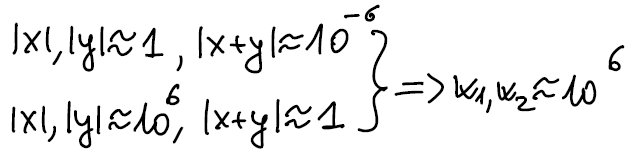
\includegraphics[scale=0.65]{foto/img12}
\end{center}
Detto a parole, due numeri dell'ordine delle unità che distano di qualche milionesimo, sono altrettante vicini in termini relativi di due numeri dell'ordine del milione che distano di qualche unità.

In entrambi i casi i pesi $w_1$, $w_2$ sono fattori di amplificazione dell'errore dell'ordine di $10^6$.\\
Possiamo sintetizzare che la SOTTRAZIONE è \uline{potenzialmente} (non sempre) \uline{INSTABILE}.\\
Infatti se $\abs{\,x\,}$ e $\abs{\,y\,}$ sono distanti in termini relativi, la sottrazione perderà poca precisione.\\
Se invece sono vicini perderà molta precisione, tanta più quanto più sono vicini.\\
Questo fenomeno (che si chiama anche “cancellazione numerica”) è il primo e importante esempio di possibile instabilità di un algoritmo (in questo caso la semplice operazione di sottrazione tra numeri approssimati).\\
È un fenomeno che studieremo meglio con degli esempi e che si può fronteggiare in 2 modi:
\begin{enumerate}
    \item cercare di riscrivere le espressioni e gli algoritmi in modo da evitare sottrazioni instabili (lo vedremo ad esempio con la formula risolutiva per le equazioni di $2^\circ$ grado)
    \item aumentando la precisione (cioè diminuendo l'errore sui dati) in funzione della grandezza di $w_1$ e $w_2$
\end{enumerate}
In campo sperimentale, questo significa aumentare la precisione dello strumento di misura. Nel caso dell'arrotondamento, questo significa andare in un sistema floating-point a precisione estesa, se ad esempio $w_1$ e $w_2$ sono così grandi da mettere in crisi un sistema a precisione doppia. Si tenga conto che come vedremo $w_1$ e $w_2$ possono essere arbitrariamente grandi e quindi far perdere completamente di significato al risultato quando $w_1, w_2 > \frac{1}{\varepsilon_M}$.\\
Come già osservato però, usare precisioni estese può avere un costo computazionale molto elevato in termini di tempo di calcolo e di occupazione di memorie.\\
Nella prossima lezione faremo vari esempi di perdita di precisione dovuta ad una sottrazione e di stabilizzazione (quando possibile) dell'algoritmo di calcolo evitando tale sottrazione.\\
Per fissare le idee, facciamo però subito un esempio significativo: 
\begin{esempio}\end{esempio}
Consideriamo la funzione
\[f(x) = \frac{((1 + x) - 1)}{x}, \quad x \ne 0\]
è evidente che $f(x) = 1$ (è la funzione costante 1) però, calcolando in Matlab $f(10^{-15})$ si ottiene $f(10^{-15}) = 1.11\dotsc$ cioè l'errore relativo sul risultato è $>11\%$ (un errore enorme rispetto all'arrotondamento che non supera $\varepsilon_M \approx 10^{-16}$)\\
Vedremo che la spiegazione sta nella sottrazione a numeratore, visto che $1+10^{-15}$ è vicinissimo ad 1.\\
Invece $f(2^{-50}) = 1$, pur essendo $2^{-50} \approx 10^{-15}$ perché?\\
Tratteremo entrambi i casi nella prossima lezione.
\newpage
\section{Lezione 5 - Esempi di instabilità della sottrazione}
Nella scorsa lezione abbiamo analizzato la risposta delle operazioni aritmetiche agli errori sui dati. \\
In particolare, dati $x, y \in \mathbb{R} \quad \Tilde{x} \approx x,\, \Tilde{y}\approx y$, i risultati ottenuti si possono sintetizzare con la disuguaglianza 
\[\varepsilon_{x \bigstar y} \le w_1\varepsilon_x + w_2\varepsilon_y\] 
dove $\varepsilon_{x \bigstar y}$ è l'errore relativo il risultato dell'operazione $\bigstar$ e $\varepsilon_x,\,\varepsilon_y$ gli errori relativi sui dati. \\
I PESI $w_1, w_2 > 0$ possono dipendere da $x,y$ (ma \uline{non} dagli errori).\\
Nel caso di moltiplicazione, divisione e addizione si ha $w_1, w_2 \approx 1$ oppure $w_1, w_2 \le 1$ quindi tali operazioni risultano STABILI.\\
Nel caso della sottrazione i pesi \[w_1 = \frac{\abs{\,x\,}}{\abs{\,x + y\,}}, \quad w_2 = \frac{\abs{\,y\,}}{\abs{\,x + y\,}}\] con $sign(x)=-sign(y)$ \uline{possono} essere invece grandi.\\
Questo accade in particolare se $x$ e $y$ sono “vicini” in termini relativi, ovvero $\abs{\,x+y\,} \ll \abs{\,x\,},\abs{\,y\,}$ quindi la SOTTRAZIONE è POTENZIALMENTE INSTABILE e in grado di diminuire in modo consistente nel risultato la precisione dei dati e anche di distruggerla completamente, rendendo il risultato praticamente privo di significato (quando $w_1,w_2 > \max \left \{ \frac{1}{\varepsilon_x},\frac{1}{\varepsilon_y} \right \}$ per cui ci si può attendere un errore $> 100\%$).\\
Faremo ora alcuni esempi significativi di perdita di precisione dovuta ad instabilità della sottrazione, lavoreremo come sempre per semplicità in sistemi floating-point virtuali in base 10.

\subsection{Esempio 1}
Consideriamo $\mathbb{F}(10,4,L,U)$ (con $L,U$ sufficienti per rappresentare i numeri che ci interessano) e \[x = 0,10016\]  \[y = -0,10012\]
allora \[\Tilde{x} = fl^4(x) = 0,1002\]  \[\Tilde{y} = fl^4(y) = -0,1001\]
eseguendo l'operazione-macchina di somma algebrica (che è una sottrazione visto che $x$ e $y$ hanno segno opposto) si ottiene
\[\begin{split}
    x \oplus y & = fl^4(fl^4(x) + fl^4(y)) \\
    & = fl^4(0,1002 -0,1001) \\
    & = 10^{-4}
\end{split}\]
scriveremo spesso i numeri in notazione standard per comodità) \\
Invece \[x+y=4 \cdot 10^{-5}\] quindi l'errore relativo nel risultato è
\[ \frac{\abs{\,(x+y)-(x+y)\,}}{\abs{\,x+y\,}} = \frac{\abs{\,4 \cdot 10^{-5} - 10^{-4}\,}}{4 \cdot10^{-5}} = \frac{6 \cdot 10^{-5}}{4 \cdot 10^{-5}} = \frac{3}{2} = 150\%\]
a fronte di $\varepsilon_x, \varepsilon_y \le \varepsilon_M = \frac{10^{-3}}{2}$ abbiamo un errore del $150\%$ e una perdita di precisione di ben 3 ordini di grandezza rispetto alla precisione di macchina.\\
Qui il problema sta nella sottrazione tra numeri vicini, visto che $x+y=4 \cdot 10^{-5}$ ma $\abs{\,x\,},\abs{\,y\,} \approx 10^{-1}$\\
Infatti se calcoliamo i pesi 
\[ w_1 = \frac{\abs{\,x\,}}{\abs{\,x+y\,}} \approx \frac{10^{-1}}{4 \cdot 10^{-5}} = \frac{10^4}{4} = 2500\] e analogamente $w_2 \approx 2500$\\
Questi fattori di amplificazione degli errori sui dati sono dell'ordine di $10^3$ e spiegano come si arrivi ad un errore finale $>100\%$, che rende inaccettabile in pratica il risultato. In questo caso i fattori di amplificazione non sono enormi, ma sono comunque $> \frac{1}{\varepsilon_M}$. \\
Osserviamo che bastava una 1 cifra di mantissa in più per avere il risultato esatto, perché con $t=5$ non ci sarebbe stato bisogno di arrotondare $x$ e $y$ e quindi $\varepsilon_x = \varepsilon_y = 0$. 
\newline \newline
Questo ci apre la strada all'analisi del prossimo esempio, un po' più sofisticato.

\subsection{Esempio 2}
Consideriamo $\mathbb{F}(10,8,L,U)$ (con $L$ e $U$ appropriati) qui $t=8$ e $\varepsilon_M = \frac{10^{-7}}{2}$. \\
Si tratta di calcolare in questa aritmetica floating-point la somma algebrica $a+b+c$ dove \[a=0,23371258 \cdot 10^{-4}\] \[b=0,33678429 \cdot 10^2\] \[c=-0,33677811 \cdot 10^2\] osserviamo che 
\[fl^8(a+b+c)=0,64137126 \cdot 10^{-3}\]
Vedremo ora che in questo esempio \uline{non} vale la proprietà \uline{associativa}, infatti
\[\begin{split}
    I & = (a \oplus b) \oplus c \\
    & = 0,33678452 \cdot 10^2 \oplus (-0,33677811 \cdot 10^2)\\
    & = 0,64100000 \cdot 10^{-3}
\end{split}\]
invece
\[\begin{split}
    II & = a \oplus (b \oplus c) \\
    & = 0,23371258 \cdot 10^{-4} \oplus 0,61800000 \cdot 10^{-3})\\
    & = 0,64137126 \cdot 10^{-3}
\end{split}\]
quindi $I \ne II$; inoltre si verifica (ad esempio in Matlab cioè sostanzialmente a 16 cifre decimali) che $II = fl^8(a+b+c)$ cioè il risultato $II$ è il meglio che si può ottenere in questa aritmetica floating-point, mentre l'errore relativo di $I$ è 
\[\frac{\abs{\,I-(a+b+c)\,}}{\abs{\,a+b+c\,}} \approx \frac{4 \cdot 10^{-7}}{0,6 \cdot 10^{-3}} = \frac{2}{3} \cdot 10^{-3} \approx 0,07\%\] 
qui riusciamo subito a spiegare la perdita di precisione di 4 ordini di grandezza rispetto a $\varepsilon_M = \frac{10^{-7}}{2}$, calcolando i pesi $w_1$ e $w_2$ associati alla \uline{sottrazione} $(a+b)+c$, visto che $a+b$ e $c$ sono vicini in termini relativi (hanno le prime 4 cifre significative coincidenti)
\[w_1 = \frac{\abs{\,x\,}}{\abs{\,x+y\,}} = \frac{\abs{\,a+b\,}}{\abs{\,a+b+c\,}} \approx\frac{0,3 \cdot 10^2}{0,6 \cdot10^{-3}} = \frac{1}{2} \cdot 10^5 = 50000\]
analogamente
\[w_2 = \frac{\abs{\,c\,}}{\abs{\,a+b+c\,}}\approx 50000\]
Si osservi che in queste stime abbiamo lavorato con 1 cifra significativa, sia con gli errori che con i pesi, perché di queste quantità non ci interessa il valore accurato ma solo l'ordine di grandezza.\\
Naturalmente, anche nel caso $II$ c'è una sottrazione che viene fatta subito, ovvero $b+c$.\\
Posto $x=b$, $y=c$ si ha \[w_1 = \frac{\abs{\,b\,}}{\abs{\,b+c\,}} \approx \frac{0,3 \cdot 10^2}{0,6 \cdot 10^{-3}} = 50000\] 
e analogamente \[w_2 = \frac{\abs{\,c\,}}{\abs{\,b+c\,}} \approx 50000\]
ma allora, perché con l'espressione di calcolo $II$ non c'è perdita di precisione?\\
La spiegazione è sottile e sta nel fatto che i numeri $a, b, c$ entrano con 8 cifre significative e non occorre arrotondarli, cioè $\varepsilon_a = \varepsilon_b = \varepsilon_c = 0$ quindi la sottrazione $b+c$ non perde precisione (invece ne perderebbe se $b$ oppure $c$ fossero arrotondati).\\
Invece, nell'espressione di calcolo $I$, la sottrazione avviene con uno dei due dati arrotondato, ovvero $a+b$, che è un'addizione il cui risultato viene comunque arrotondato perché ha più di 8 cifre significative (cifre di mantissa) e quell'errore di arrotondamento viene amplificato dal peso $w_1$ (mentre il peso $w_2$ moltiplica $\varepsilon_c = 0$ e quindi non ha effetto).\\
Osserviamo che in una sottrazione instabile \uline{basta che uno dei due dati sia affetto da errore} per vedere la perdita di precisione.\\
Siamo in grado a questo punto di discutere l'esempio portato alla fine della lezione 4, rispondendo alle domande: perché $f(10^{-15})$ in Matlab ha un errore $>11\%$ e $f(2^{-50})$ è “esatto”?
 
\subsection{Esempio 3}
Si consideri il calcolo in Matlab della funzione
\[f(x) = \frac{(1+x)-1}{x} \quad , \quad x \ne 0\]
Chiaramente $f(x) \equiv 1$ (è la funzione costante 1), in Matlab però con le operazioni-macchina si calcola 
\[\Tilde{f}(x) = \bigl( (1 \overbrace{\oplus}^{\text{ADD}} x) \overbrace{\oplus}^{\text{SOTTR}} (-1) \bigr) \overbrace{\oslash}^{\text{DIV}} x\]
e si ha \[\Tilde{f}(10^{-15}) = 1,11 \dotsc\] 
cioè l'errore relativo nel calcolo di $f$ è
\[\varepsilon_{f(x)} = \frac{\abs{\,f(x) - \Tilde{f}(x)\,}}{\abs{\,f(x)\,}} = \abs{\,1 - 1,11 \dotsc\,} = 0,11 \dotsc > 11\%\]
La spiegazione sta nella sottrazione che avviene tra due numeri estremamente vicini, cioè $1 + x$  e  1 (invece le altre operazioni, un'addizione e una divisione, sono stabili) mentre 1 è un reale-macchina e non viene quindi arrotondato, $x=10^{-15}$ viene arrotondato (non lo sarebbe se la base fosse 10, ma non bisogna mai dimenticare che in Matlab la base vera è 2), così come $1 + 10^{-15}$.\\
Questi piccolissimi errori di arrotondamento (ricordiamo che sono $\le 2^{-53} \approx 10^{-16}$) vengono però amplificati dal peso $w_1$ nella sottrazione $(1 + x) - 1$, $x = 10^{-15}$.\\
Calcoliamo
\[w_1 = \frac{\abs{\,1+x\,}}{\abs{\,(1+x)-1\,}} = \frac{1+x}{x} \approx 10^{15}\]
che spiega perfettamente come si siano persi 15 ordini di grandezza nel calcolo di $f$.\\
Dall'altra parte il peso $w_1$ nel caso della sottrazione $(1+x)-1$, $x=2^{-50} \approx 10^{-15}$ è sempre dell'ordine di $10^{15}$.\\
Per quale motivo allora $\Tilde{f}(2^{-50}) = 1$, cioè in questo caso il risultato è esatto?\\
Perché $2^{-50}$ e $1+2^{-50}$ sono entrambi reali-macchina in base 2 e perciò \uline{non} vengono arrotondati, cioè 
\[\varepsilon_{1+x} = \frac{\abs{\,(1+x)-(1\oplus x)\,}}{(1+x)} = 0\]
e il fattore di amplificazione non ha effetto.\\

Come ultimo esempio di possibile instabilità della sottrazione ci occuperemo ora della formula risolutiva per le equazioni di $2^\circ$ grado, formula che siamo abituati ad usare senza farci problemi.\\
Scopriremo invece che in certe situazioni questa formula in aritmetica floating-point può perdere moltissima precisione, fino a far perdere del tutto di significato al risultato vedremo però anche che la formula può essere convenientemente “stabilizzata” eliminando la sottrazione potenzialmente instabile.

\subsection{Esempio 4}
Consideriamo un'equazione di grado effettivo 2 \[az^2+bz+c=0 \quad , \quad a \ne 0\]
nel caso di discriminante \[\Delta = b^2 -4ac >0\] 
le cui soluzioni si scrivono abitualmente come \[z_{\pm} = \frac{-b \pm \sqrt{\Delta}}{2a}\]
Ora, una di queste due soluzioni richiede una sottrazione, ovvero $z_+$ per $b>0$ e $z_-$ per $b <0 $: \uline{prendiamo per semplicità $b>0$}, essendo l'analisi dell'altro caso del tutto analoga. Osserviamo che in aritmetica floating-point $\sqrt{\Delta}$ sarà quasi sempre arrotondato, d'altra parte la funzione $\sqrt{\cdot}$ viene calcolata alla precisione di macchina in tutti i linguaggi di calcolo (vedremo nelle prossime lezioni un metodo rapido per calcolare $\sqrt{\alpha}$, $\alpha>0$ come soluzione dell'equazione $x^2-\alpha = 0$, il metodo delle tangenti detto anche metodo di Newton) quindi nella sottrazione $\sqrt{\Delta} -b$ il primo dato è sicuramente affetto da un errore al massimo dell'ordine della precisione di macchina.\\
Quando ci si aspetta che questa sottrazione possa far perdere precisione? Quando $\sqrt{\Delta}$ è vicina a $b$ in termini relativi, cioè per 
\[b^2 \gg \abs{\,4ac\,} \Longrightarrow \sqrt{\Delta} \approx b\]
Infatti posto $x = \sqrt{\Delta}$, $y = -b$, i pesi sono
\[w_1 = \frac{\abs{\,x\,}}{\abs{\,x+y\,}} = \frac{\sqrt{\Delta}}{\abs{\,\sqrt{\Delta}-b\,}} = \frac{\sqrt{\Delta}\cdot (\sqrt{\Delta}+b)}{\abs{\,\sqrt{\Delta}-b\,}\cdot (\sqrt{\Delta}+b)} = \frac{\sqrt{\Delta}\cdot (\sqrt{\Delta}+b)}{\abs{\,\Delta - b^2\,}} = \frac{\sqrt{\Delta}\cdot (\sqrt{\Delta}+b)}{\abs{\,b^2 - (b^2-4ac)\,}}\]
Ma $\sqrt{\Delta} \approx b$ quindi
\[w_1 = \frac{\sqrt{\Delta}\cdot (\sqrt{\Delta}+b)}{\abs{\,4ac\,}} \approx \frac{2b^2}{\abs{\,4ac\,}} = \frac{b^2}{2 \cdot\abs{\,ac\,}}\]
e analogamente
\[w_2 = \frac{\abs{\,-b\,}}{\abs{\,\sqrt{\Delta}-b\,}} = \frac{b\cdot (\sqrt{\Delta}+b)}{\abs{\,4ac\,}} \approx \frac{b^2}{2 \cdot\abs{\,ac\,}}\]

Siccome il rapporto $\frac{b^2}{2 \cdot\abs{\,ac\,}}$ può diventare arbitrariamente grande (dipende dagli ordini di grandezza dei coefficienti $a, b, c$) la soluzione $z_+$ può subire una fortissima perdita di precisione in aritmetica floating-point, fino a renderla priva di significato in pratica.\\ 
Facciamo a questo proposito un paio di esempi 

\subsection{Esempio 4.1}
Consideriamo l'equazione \[z^2 + 100z -1 = 0\]
cioè $a = 1$, $b= 100$, $c =-1$ con $\Delta = 100^2+4= 10004$\\
Nel sistema floating-point virtuale $\mathbb{F}(10, 4, L, U)$ con $L$ ed $U$ opportuni (qui il parametro chiave è $\#$cifre mantissa = 4) con $t=4$ cifre di mantissa $\Delta$ viene arrotondato a 10000
\[fl^4(\Delta) = fl^4(0,10004)\cdot 10^5=(0,1000)\cdot 10^5\]
quindi viene calcolato $\sqrt{\Delta} = 100$ (come sempre, usiamo il meno possibile la notazione floating-point per semplicità)\\
Quindi in questo sistema viene calcolata $\Tilde{z}_+ = 0$ con un errore relativo del $100\%$
\[\frac{\abs{\,z_+ - \Tilde{z}_+\,}}{\abs{\,z_+\,}} = \frac{\abs{\,z_+\,}}{\abs{\,z_+\,}} = 1\]
In un certo senso questo è un caso limite, per la scarsità di cifre di mantissa si è costretti ad approssimare con 0 una quantità che non è nulla, facendo direttamente un errore relativo del $100\%$.\\
Per vedere l'effetto dei coefficienti di amplificazione
\[w_1,w_2 \approx \frac{b^2}{2\,\abs{\,ac\,}} \approx \frac{10^4}{2} = 5000\]
Consideriamo $\mathbb{F}(10,8,L,U)$ cioè passiamo a $t=8$ cifre di mantissa con $\varepsilon_M = \frac{10^{-7}}{2}$\\ 
In questo caso si può verificare che
\[ \Tilde{z}_+ = \frac{-100 + \sqrt{10004}}{2} = \frac{-100 + 100,02000}{2} = 10^{-2} \]
mentre il valore “esatto” è \[z_+= 0.0099990002\] per cui abbiamo un errore relativo
\[\frac{\abs{\,z_+ - \Tilde{z}_+\,}}{\abs{\,z_+\,}} \approx 10^{-4}\]
Abbiamo quindi perso 3 ordini di precisione rispetto alla precisione di macchina, il che è ben spiegato dai pesi $w_1, w_2$ che sono dell'ordine di $10^3$.\\ Osserviamo che l'errore commesso è $\approx 10^{-4}$, cioè circa dello $0.01\%$.\\ 
D'altra parte tale errore, che potrebbe essere comunque accettabile in molti contesti applicativi, è 2000 volte più grande della precisione di macchina (poteva esserlo fino a 5000 volte, ma va tenuto presente che la precisione di macchina è una soglia massima e che gli errori relativi sono di solito più piccoli di essa).\\
Se avessimo lavorato con $t=16$ cifre di mantissa, ci saremmo aspettati un'amplificazione degli errori di arrotondamento fino a
\[5000 \cdot\varepsilon_M = 5000 \cdot \frac{10^{-15}}{2} \approx 10^{-12}\]
e quindi avremmo ottenuto una precisione $< \varepsilon_M$ ma comunque molto elevata. Ma non è difficile convincersi che ci vuole poco per mettere in crisi qualsiasi sistema floating-point, basta che cambino i rapporti tra gli ordini di grandezza dei coefficienti.

\subsection{Esempio 4.2 - Soluzione di equazioni di secondo grado}
Consideriamo infatti 
\[10^{-2}z^2 + 10^4z + 10^{-2} = 0\]
in $\mathbb{F}(10,16,L,U)$ (sostanzialmente la precisione dell'interfaccia del Matlab).\\
Si osservi che qui con $t=8$ cifre di mantissa saremmo stati di nuovo nella situazione di approssimare $\Delta = 10^8 - 4 \cdot 10^{-4}$ con $10^8$, perché $\Delta$ ha 12 cifre significative 
\[\Delta = (0,\underbrace{100 \dotsc 04}_{\text{12 cifre}}) \cdot 10^9\]
facendo quindi un errore relativo del $100\%$.\\
Con $t=16$ cifre di mantissa si calcola
\[\Tilde{z}_+ = \frac{-10^4 + \sqrt{10^8 - 4 \cdot 10^{-4}}}{2 \cdot 10^{-2}} = -(0,9999894 \dotsc 46) \cdot 10^{-6}\]
mentre la soluzione “esatta” (arrotondata a 16 cifre) è \[z_+ = -(0.1000000000001000)\cdot 10^{-5}\] con errore relativo
\[\frac{\abs{\,z_+ - \Tilde{z}_+\,}}{\abs{\,z_+\,}} \approx \frac{1.1 \cdot 10^{-5} \cdot 10^{-6}}{10^{-6}} = 1.1 \cdot 10^{-5}\]
e una perdita di precisione di 10 ordini di grandezza rispetto a $\varepsilon_M = \frac{10^{-15}}{2}$,che è spiegabile con i fattori di amplificazione
\[w_1,w_2 \approx \frac{b^2}{2\,\abs{\,ac\,}} = \frac{10^8}{2 \cdot 10^{-4}} = \frac{1}{2} \cdot 10^{12}\]
questi esempi mostrano che la formula risolutiva classica delle equazioni di $2^\circ$ grado è molto instabile quando \[b^2 \gg 4\,\abs{\,ac\,}\] 
(ovvero $\sqrt{\Delta} \approx \abs{\,b\,}$), a causa di una sottrazione intrinseca nel modo in cui è scritta.\\
In questo caso però il problema si può risolvere riscrivendo la formula con un “trucchetto” algebrico. \\
Considerando nuovamente il caso $b>0$ 
\[z_+ = \frac{\sqrt{\Delta}-b}{2a} = \frac{(\sqrt{\Delta}-b)(\sqrt{\Delta}+b)}{2a(\sqrt{\Delta}+b)} = \frac{\Delta -b^2}{2a(\sqrt{\Delta}+b)} = \frac{-4ac}{2a(\sqrt{\Delta}+b)} = - \frac{2c}{\sqrt{\Delta}+b}\] 
in $\mathbb{R}$ le 2 formule sono equivalenti; in $\mathbb{F}$ invece, la formula 
\[z_+ = - \frac{2c}{\sqrt{\Delta}+b}\]
diventa stabile perché è stata eliminata la sottrazione (che come sappiamo è instabile per $b^2 \gg 4\,\abs{\,ac\,}$). \\
D'altra parte, 
\[z_- = - \frac{(b+\sqrt{\Delta})}{2a}\]
è \uline{stabile} perché non contiene sottrazioni.\\
Possiamo a questo punto scrivere una formula risolvibile “STABILIZZATA” che tiene conto del segno di $b$, ovvero
\[ \begin{cases}
    z_1 = - sign(b)\frac{2c}{\abs{\,b\,} + \sqrt{\Delta}} \\
    z_2 = - sign(b)\frac{\abs{\,b\,} + \sqrt{\Delta}}{2a}
\end{cases}\]
Tornando all'esempio 4.2 , si ha che $\Tilde{z}_+$ fa un errore relativo $\approx 10^{-5}$ su $z_+$ come abbiamo visto, mentre detto $\Tilde{z}_1$ il valore di $z_1$ calcolato in $\mathbb{F}$, si ha $\Tilde{z}_1 = fl^{16}(z_+)$ cioè il calcolo di $z_+$ è stato completamente stabilizzato.\\
Qualcuno potrebbe osservare che anche il calcolo di $\Delta$ può contenere una sottrazione, precisamente quando $sign(a)=sign(c)$ e che questa può diventare instabile quando $b^2 \approx 4ac$ o meglio quando 
\[\abs{\,b^2 - 4ac\,} \ll b^2,4ac\]
Questa situazione è molto più difficile da trattare e non ce ne occuperemo.\\ Diciamo solo che qui la perdita di precisione non è completamente eliminabile, ma esiste un algoritmo grazie al quale l'errore relativo sulle due soluzioni per $\Delta>0$ con $b^2 \approx 4ac$ è dell'ordine di $\varepsilon_M^{\frac{1}{3}}$ (dove $\varepsilon_M$ è la precisione di macchina) cioè con perdita di precisione consistente ma controllata.
\newpage
\section{Lezione 6 - Condizionamento delle funzioni, propagazione degli errori}
\subsection{Indice di condizionamento}
In questa lezione ci occuperemo di due aspetti importanti del calcolo approssimato, tramite esempi: l'effetto degli errori sulla variabile $x$ e degli errori di arrotondamento nel calcolo dei valori di una funzione $f(x)$, e l'effetto degli errori di arrotondamento in un algoritmo iterativo che costruisce i valori di una successione convergente alla quantità da approssimare.\\
Cominciamo col calcolo di funzioni, visto che in pratica tutte le quantità utilizzate nel calcolo sono approssimate, possiamo innanzitutto porci la seguente domanda: qual è l'effetto sul valore di $f$ di un errore sulla variabile indipendente $x$? Cioè, come risponde $f$ agli errori?\\
Come sempre, siamo maggiormente interessati agli errori relativi. Consideriamo una funzione $f: I \to \mathbb{R}$ dove $I$ è un intervallo e $x, \tilde{x} \in I$ dove $\tilde{x} \approx x, x \neq 0$ con errore relativo
\[\varepsilon_x = \frac{\abs{\,x-\tilde{x}\,}}{\abs{\,x\,}}\]
Cerchiamo di stimare $\varepsilon_{f(x)}$\\
\[ \varepsilon_{f(x)} = \frac{\abs{\,f(x)-f(\tilde{x})\,}}{\abs{\,f(x)\,}}, \quad f(x) \neq 0 \]
Supponendo $f$ \uline{derivabile} in $I$ possiamo utilizzare la formula
di Taylor al primo ordine centrata in $x$
\[ f(\tilde{x}) \approx f(x) + f'(x)\cdot (\tilde{x}-x) \]
da cui ricaviamo
\[ f(\tilde{x})-f(x) \approx f'(x)\cdot (\tilde{x}-x) \iff
        \frac{\abs{\,f(\tilde{x})-f(x)\,}}{\abs{f(x)}} \approx \frac{\abs{\,f'(x)\,}}{\abs{\,f(x)\,}} \cdot \abs{\,\tilde{x}-x\,} = \frac{\abs{\,f'(x)\,} \cdot \abs{\,x\,}}{\abs{\,f(x)\,}} \cdot \frac{\abs{\,\tilde{x}-x\,}}{\abs{\,x\,}} \]
che possiamo riassumere con \[\varepsilon_{f(x)} \approx condf(x) \varepsilon_x \] dove
\[ condf(x)=\frac{\abs{\,f'(x)\,} \cdot \abs{\,x\,}}{\abs{\,f(x)\,}} \]
è l'\uline{INDICE DI CONDIZIONAMENTO} di $f$ in $x$ ed è la quantità che permette di misurare la risposta di $f$ ad errori su $x$.\\
Se l'indice di condizionamento è grande, la funzione risulta instabile (o ``\uline{mal condizionata}"), nel senso che l'errore sulla variabile viene amplificato.\\
Questo è il primo esempio che incontriamo di ``problema instabile" (o ``problema mal condizionato") che si può definire in modo empirico come un problema in cui ``piccoli errori sui dati possono portare ad errori grandi sulla soluzione".\newline \newline
La stabilità del problema è un concetto che va tenuto ben distinto da quello di stabilità di un algoritmo che ne calcola la soluzione, come vedremo negli esempi seguenti.
\subsection{Esempi}
Cominciamo con un esempio che ben conosciamo: \newline
\begin{esempio}
\[ f(x)=\frac{(1+x)-1}{x}, \quad x \neq 0 \] \end{esempio}
Chi è questa funzione? È la funzione costante 1, che ovviamente risponde in modo ottimale agli errori su $x$, visto che ovunque vale 1, quindi \[\varepsilon_{f(x)}=0 \quad \forall x,\tilde{x}\] 
e in effetti \[f'(x)=0 \quad \forall x \Rightarrow cond f(x)=0 \quad \forall x\]
Sappiamo però anche che in aritmetica floating-point il calcolo di $f$ è instabile se usiamo la formula scritta sopra per $\abs{\,x\,}$ piccolo.\\
Infatti per $x\rightarrow 0$ il peso
\[ w_1=\frac{\abs{\,1+x\,}}{\abs{\,(1+x)-1\,}}=\frac{\abs{\,1+x\,}}{\abs{\,x\,}}\rightarrow +\infty \] \newline \newline
Nella sottrazione $(1+x)-1$, più piccolo è $\abs{\,x\,}$, più la formula è instabile a causa della perdita di precisione nella sottrazione
(sappiamo, ad esempio, che in Matlab $f(10^{-15})=1.11 \dotsc$ con un errore relativo $>11\%$ spiegato dal fatto che $w_1\approx 10^{-15}$)\\
Ma ATTENZIONE: è la formula, cioè l'espressione di calcolo, cioè l'\uline{algoritmo}, ad essere \uline{instabile} invece la \uline{funzione} è perfettamente \uline{stabile} e potremmo calcolarla con un algoritmo stabile, ovvero semplicemente $f(x)=1$\\
Chiaramente si tratta di un caso limite, adesso vedremo altri esempi meno estremi
\begin{itemize} %1
    \item $f(x)=\frac{1}{x},\quad x\neq 0$
\end{itemize}
\[cond f(x)= \frac{\abs*{\,-\frac{1}{x^2}\,} \cdot \abs{\,x\,}}{\abs*{\,\frac{1}{x}\,}} = 1 \]
questa è una funzione stabile $\forall x$, in effetti lo sappiamo già, è l'operazione di reciproco \newline

\begin{itemize} %2
    \item $f(x)=1-x$
\end{itemize}
\[ cond f(x)= \frac{\abs{\,(-1)\,}\abs{\,x\,}}{\abs{\,1-x\,}} = \frac{\abs{\,x\,}}{\abs{\,1-x\,}} \] 
ora $cond f(x)\rightarrow +\infty, \quad x\rightarrow 1$ quindi la funzione è instabile per $x\approx$ 1.\\
Di nuovo non è una sorpresa, si tratta di una sottrazione instabile per $x\approx1$, qui $condf(x)=w_2$ \newline

\begin{itemize} %3
    \item $f(x) = 1-\sqrt{1-x^2}, \quad 0 < \abs{\,x\,} \le 1$\\
\end{itemize}
\[ f'(x) = -\,\frac{1}{2\sqrt{1-x^2}} \cdot (-2x) = \frac{x}{\sqrt{1-x^2}} \]
\begin{center}
    (derivata di una funzione composta)
\end{center}
e quindi
\[ \begin{split}
        condf(x) & = \frac{\abs{\,x\,}}{\sqrt{1-x^2}} \cdot \frac{\abs{\,x\,}}{\abs{\,f(x)\,}} \\
        & = \frac{x^2}{\sqrt{1-x^2}} \cdot \frac{1}{1-\sqrt{1-x^2}} \\
        & = \frac{x^2}{\sqrt{1-x^2}}\cdot \frac{1 + \sqrt{1-x^2}}{(1 + \sqrt{1-x^2})(1 - \sqrt{1-x^2})}\\
        & = \frac{x^2(1+\sqrt{1-x^2})}{\sqrt{1-x^2}(1-(1-x^2))} \\
        & = \frac{1+\sqrt{1-x^2}}{\sqrt{1-x^2}} \\
    \end{split} \]
Abbiamo che
\[ condf(x)\rightarrow2, \quad x\rightarrow0 \]
Quindi $f$ è ben condizionata per $x\approx0$.\\ 
D'altra parte il calcolo con l'espressione
\[ f(x)=1-\sqrt{1-x^2} \]
è instabile per $x\approx 0$ a causa della sottrazione esterna 
\[1 \underset{\underset{\text{\tiny{INSTAB.}}}{\uparrow}}{-} \sqrt{1 \underset{\underset{\text{\tiny{STAB.}}}{\uparrow}}{-} x^2} \quad \text{per } x \approx 0\]
mentre la sottrazione sotto radice è stabile.\\
Il motivo è che nella sottrazione interna i due numeri si allontanano in termini relativi per $x \to 0$, mentre in quella esterna si avvicinano, infatti
\[ w_2 = \frac{\sqrt{1-x^2}}{1-\sqrt{1-x^2}} = \frac{\sqrt{1-x^2}\cdot (1+\sqrt{1-x^2})}{x^2} \to +\infty \]
per $x\to 0$.\\
Cosa stiamo vedendo? La funzione è stabile per $x\approx 0$, ma l'algoritmo scelto per calcolarla non lo è (a causa della sottrazione esterna). Dai conti fatti con le equazioni di $2^\circ$ grado, sappiamo però che possiamo stabilizzare la formula per il calcolo di $f$
\[ \begin{split}
    f(x) & = 1-\sqrt{1-x^2} \\
    & = \frac{(1-\sqrt{1-x^2}) \cdot (1+\sqrt{1-x^2})}{1+\sqrt{1-x^2}} \\
    & =\frac{1-(1-x^2)}{1+\sqrt{1-x^2}} \\
    & =\frac{x^2}{1+\sqrt{1-x^2}} 
\end{split} \]
Con questa seconda formula il calcolo in aritmetica di macchina diventa stabile per $x \approx 0$, perché tutte le operazioni coinvolte (potenza, divisione, addizione e sottrazione sotto radice) sono stabili.\\
La risposta di una funzione ad errori sulla variabile è una proprietà intrinseca della funzione, potremmo dire una proprietà ``strutturale", che non dipende da ``come" è scritta ma solo dall'indice di condizionamento $cond f(x)$.\\ 
D'altra parte ``come" è scritta significa qual è l'$\uline{algoritmo}$ di calcolo.\\
Abbiamo visto che per una funzione ben condizionata possono esserci algoritmi stabili e algoritmi instabili, sta a noi sceglierne uno stabile.\\ 
Usando di nuovo una definizione non rigorosa ma empirica possiamo dire che un algoritmo è instabile quando \textit{``piccoli errori introdotti durante il processo di calcolo (ad esempio gli arrotondamenti in aritmetica floating-point) possono portare ad errori grandi sui risultati del calcolo"}.\\
\newline
Siccome nel calcolo di $f(x)$ un errore su $x$ (misura sperimentale, arrotondamento, $\dotsc$) cioè sul dato del problema, è uno degli errori introdotti nel processo di calcolo, ci si aspetta che se esiste un algoritmo stabile la funzione sia ben condizionata, cioè che $condf(x)$ non sia grande.\\ 
È proprio quello che accade nell'esempio precedente, dove la scrittura 
\[f(x) = \frac{x^2}{1+\sqrt{1-x^2}}\] è stabile per $x\approx 0$, infatti $condf(x)\approx 2$ (cioè non è grande) per $x\approx 0$.\\
Viceversa, se una funzione è instabile (mal condizionata) ci aspettiamo che qualsiasi algoritmo di calcolo ``erediti" questa instabilità.\\
È bene ribadire che tutti questi concetti (non facili) li stiamo esprimendo in modo empirico ed essenzialmente qualitativo, per non entrare nell'ambito di teorie generali della stabilità che richiedono strumenti matematici di livello superiore a quelli che usiamo in questo corso.\\
\newline
Per concludere con l'esempio, osserviamo che $f(x) = 1-\sqrt{1-x^2}$ è ben condizionata per $x \approx 0$, ma è mal condizionata per $\abs{\,x\,} \approx 1$ visto che \[condf(x) = \frac{1+\sqrt{1-x^2}}{\sqrt{1-x^2}} \to +\infty \] 
per $\abs{\,x\,} \to 1$.\newline \newline
Nella seconda parte della lezione facciamo un passo ulteriore verso una metodologia caratteristica del calcolo numerico, ovvero il calcolo di una successione che \uline{converge} alla quantità che vogliamo approssimare, tramite un \uline{algoritmo iterativo}.\\
Il problema che affrontiamo è il calcolo di $\pi$ in un sistema floating-point a 64 bit (ad esempio in Matlab) con un errore dell'ordine della precisione di 
macchina (cioè con almeno 15 cifre corrette nell'interfaccia in base 10).

\subsection{Calcolo di $\pi$}
\subsubsection{Serie armonica}
Consideriamo 2 successioni convergenti a $\pi$:\\
la prima si può ottenere dal fatto che la cosiddetta serie armonica (con esponente 2) converge e ha come somma
\[ \sum_{k=1}^\infty \frac{1}{k^2} = \frac{\pi^2}{6} \]
(risultato che accettiamo senza dimostrarlo).\\
Allora, detta \[S_n = \sum_{k=1}^n \frac{1}{k^2}\] la somma parziale n-esima, visto che 
\[ \sum_{k=1}^\infty \frac{1}{k^2} = \lim_{n \to \infty} S_n = \frac{\pi^2}{6} \] si ottiene subito \[\lim_{n \to \infty} \sqrt{6\cdot S_n} = \pi \]
Osserviamo che il calcolo di $S_n$ in aritmetica di macchina è stabile, perché coinvolge solo operazioni stabili (elevamento al quadrato, reciproco, addizioni essendo la serie a termini positivi) però la successione $\sqrt{6\cdot S_n}$ è
in pratica inutilizzabile per calcolare $\pi$ con grande precisione, perché la successione $S_n$ converge troppo lentamente.\\
Infatti si vede con il criterio di confronto integrale che il resto 
\[ \frac{\pi^2}{6} - S_n = \sum\limits_{k=n+1}^\infty \frac{1}{k^2} \] 
si può maggiorare nel modo seguente
\[ \sum_{k=n+1}^\infty \frac{1}{k^2} < \int_n^\infty \frac{1}{x^2} dx = \frac{1}{n} \]
come è chiaro dal disegno schematico (non in scala)\\
\begin{center}
    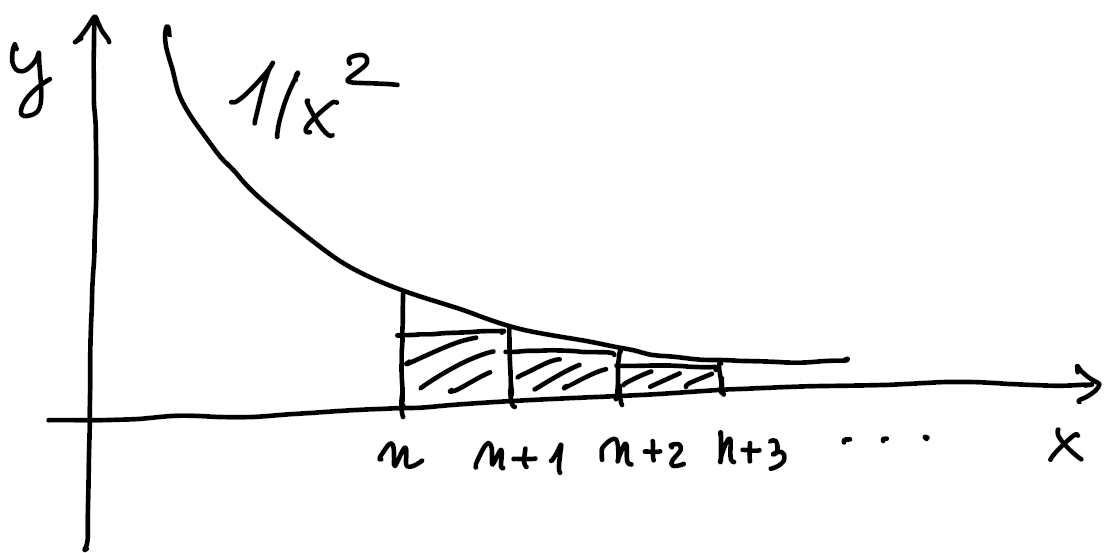
\includegraphics[width=0.6\textwidth]{foto/img13}
\end{center}
dove si vede che l'area che sta sotto la curva $y= \frac{1}{x^2}$ tra $n$ e $\infty$ (cioè $\int_n^\infty \frac{1}{x^2}dx$) è maggiore della somma delle aree dei rettangolini che hanno base 1 e altezza $\frac{1}{k^2}$ con $k = n+1, n+2, \dotsc$ cioè $\sum_{k=n+1}^\infty \frac{1}{k^2}$. \\
Quindi l'errore che si commette approssimando $\frac{\pi^2}{6}$ con $S_n$ si può stimare con \[ \frac{\pi^2}{6}-S_n < \frac{1}{n} \]
Questo significa che per approssimare $\frac{\pi^2}{6}$ con un errore $\le \varepsilon_M$ (precisione di macchina) basta che 
\[\frac{\pi^2}{6}-S_n < \frac{1}{n} \le \varepsilon_M \]
cioè $n \ge \varepsilon_M^{-1} \approx 10^{16}$, quindi bisognerebbe sommare $10^{16}$ (10 milioni di miliardi) di termini della serie!\\
D'altra parte in aritmetica di macchina ad un certo punto la somma $S_n$ diventerebbe costante, perché i termini che vanno sommati diventerebbero troppo piccoli e si comporterebbero come elementi neutri, impedendo di raggiungere la precisione richiesta (accade da $n\approx10^8$ in poi).

\subsubsection{Successione di Archimede}
Considerando invece la successione definita ``per ricorrenza" da\\\\
$x_0=2$\\
$x_{n+1}=2^{n-\frac{1}{2}}\cdot\sqrt{1-\sqrt{1-(4^{1-n})x_{n}^2}}, \quad n=2,3,4,\dotsc$\\
detta ``successione di Archimede" si può dimostrare con metodi geometrici (legati all'approssimazione del cerchio con poligoni regolari) che 
\[ \lim_{n\to\infty} x_n= \pi \]
Se calcoliamo $x_n$ in Matlab con un semplice ciclo ``for" e plottiamo l'errore relativo \[ r_n=\frac{\abs{\,\tilde{x}_n-\pi\,}}{\pi} \] in SCALA LOGARITMICA , cioè plottiamo $log_{10}(r_n)$, otteniamo un grafico tipo quello disegnato di seguito in nero
\begin{center}
    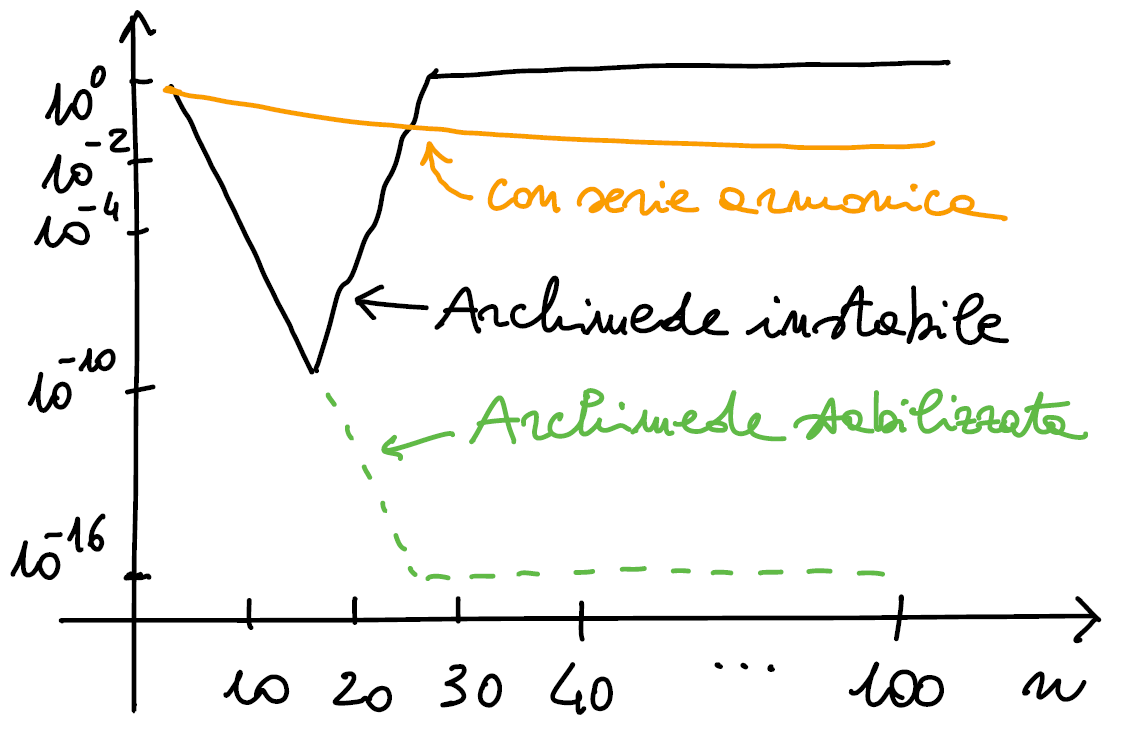
\includegraphics[width=0.5\textwidth]{foto/img14}
\end{center}
(dove abbiamo interpolato i valori discreti per una migliore visualizzazione).\\
Si vede che l'errore decresce linearmente fino a circa $10^{-10}$ e poi comincia a crescere, cioè la successione $\tilde{x}_n$ calcolata con lo schema descritto sopra in aritmetica di macchina da un certo $n$ in poi comincia ad allontanarsi da $\pi$.\\
Si noti che fino a quel punto l'errore decade rapidamente, infatti un decadimento lineare in scala logaritmica significa che 
\[ log_{10}(r_n)=-\alpha\,n+\beta \quad \text{ con } \alpha >0 \] 
cioè in scala normale 
\[r_n=10^{-\alpha n+\beta}=\gamma\,\theta^n \quad \text{ con } \quad \gamma=10^{\beta} \quad \text{ e } \quad \theta=10^{-\alpha}< 1 \] 
che è un decadimento esponenziale (tanto più veloce quanto più grande è $\alpha$).\\
È chiaro che l'algoritmo è instabile e che tale instabilità è in grado da un certo $n$ in poi di distruggere la convergenza della successione (si osservi però che comunque la convergenza finché c'è è rapida e permette di arrivare ad approssimare $\pi$ con un errore $\approx10^{-10}$ in meno di 20 iterazioni).\\ 
A cosa è dovuta l'instabilità? All'interno della radice quadrata esterna ci sono 2 sottrazioni, 
\[ 1-\sqrt{1-\alpha_n} \quad \text{ con } \alpha_n=(4^{1-n})x^{2}_n \]
Visto che $\alpha_n$ è un infinitesimo, $\alpha_n \to 0,\, n\to\infty$ (perché $4^{-n}\to 0$ e $x^{2}_n\to\pi^2,\, n\to\infty$) la sottrazione $1-\alpha_n$ è stabile (i numeri si allontanano in termini relativi al crescere di $n$).\\ 
Ma per lo stesso motivo la sottrazione 
\[ 1-\sqrt{1-\alpha_n} \] 
diventa sempre più instabile al crescere di $n$, perché $\sqrt{1-\alpha_n}\to1$, $n\rightarrow\infty$ e la convergenza a 1 è rapida ($\abs{\,1-\sqrt{1-\alpha_n}\,}$ va a zero come $4^{-n}$).\\
Possiamo calcolare il peso $w_2$ di questa sottrazione, visto che $\sqrt{1-\alpha_n}$ è sicuramente affetto da errore (dell'ordine della precisione di macchina, visto che $\sqrt{\,\cdot\,}$ è una funzione predefinita calcolata alla precisione di macchina).\\ 
Posto $x=1,\, y=-\sqrt{1-\alpha_n}$ si ha\\
\[\begin{split}
    w_2 & = \frac{\abs{\,y\,}}{\abs{\,x+y\,}} \\
    & = \frac{\sqrt{1-\alpha_n}}{1-\sqrt{1-\alpha_n}} \\
    & = \frac{\sqrt{1-\alpha_n}(1+\sqrt{1-\alpha_n})}{(1-\sqrt{1-\alpha_n})(1+\sqrt{1-\alpha_n})} \\
    & =\frac{\sqrt{1-\alpha_n}(1+\sqrt{1-\alpha_n})}{1-(1-\alpha_n)} \\
    & \approx\frac{2}{\alpha_n}=2\cdot\frac{4^{n-1}}{x^{2}_n}\approx\frac{1}{2\pi^2}4^n
\end{split}\]
Quindi il peso $ w_2 $ è fattore di amplificazione che cresce esponenzialmente come $ 4^n $.\\
Possiamo stimare l'errore $ e_n=\abs{\,\pi - \Tilde{x}_n\,} $ in questo modo:
\[\begin{split}
    e_n & = \abs{\,\pi - x_n + x_n - \Tilde{x}_n\,} \\
    & \le \underbrace{\abs{\,\pi - x_{n}\,}}_{\text{\tiny{CONVERGENZA}}} + \underbrace{\abs{\,x_n - \Tilde{x}_n\,}}_{\text{\tiny{STABILITÀ}}}
\end{split}\]
dove l'errore $\abs{\,\pi - x_{n}\,}$ è legato alla \uline{convergenza teorica} del metodo (in generale, dire che
\[\lim_{x\to \infty} x_{n} = l\]
con $l$ limite finito è equivalente a dire che l'errore $\abs{\,x_n - l\,}\to 0,\, n \to \infty $), mentre l'errore $\abs{\,x_n - \Tilde{x}_n\,}$ è legato alla \uline{stabilità dell'algoritmo} che implementa il metodo. \\
Dall'analisi fatta, 
\[\abs{\,x_n - \pi\,} = c\,\theta^{n} \quad \text{ con } 0<\theta<1\] mentre 
\[\abs{\Tilde{x}_n - x_n} \lesssim c' \cdot 4^n\,\varepsilon_{M}\] 
con $c$ e $c'$ costanti. Quindi 
\[ e_n \lesssim c\,\theta^n + c' \, 4^n\,\varepsilon_{M} \]
da cui ci aspettiamo che finché 
\[c'\,4^{n}\,\varepsilon_{M}<c\,\theta^{n}\] 
si continui a vedere la convergenza, ma da quel punto in poi il termine esponenziale crescente comincia a sovrastare e in pratica fa allontanare la successione calcolata dal limite. \\
Si osservi che ad un certo punto l'errore diventa costante: questo accade quando $\alpha_n$ è così piccolo che $1 \ominus \alpha_n = 1$ e quindi $\tilde{x}_n=0$ forzando un errore del $100\%$.\\
È però possibile stabilizzare il calcolo di $x_n$ eliminando la sottrazione instabile, con lo stesso trucco utilizzato per le equazioni di $2^\circ$ grado. \\
Il cuore del problema è infatti il calcolo di  $1-\sqrt{1-\alpha_{n}}$ :
\[\begin{split}
    1-\sqrt{1-\alpha_{n}} & = \frac{(1-\sqrt{1-\alpha_n})(1+\sqrt{1-\alpha_n})}{1+\sqrt{1-\alpha_n}} \\
    & = \frac{1-(1-\alpha_n)}{1+\sqrt{1-\alpha_n}} \\ 
    & = \frac{\alpha_n}{1+\sqrt{1-\alpha_n}}
\end{split}\]
questa riscrittura è stabile in aritmetica floating-point, perché sono coinvolte solo operazioni stabili.\\
Possiamo allora riscrivere l'iterazione in forma stabile 
\[\begin{split}
    x_{n+1} & = 2^{n-\frac{1}{2}}\sqrt{1-\sqrt{1-\alpha_n}} \quad \Longleftarrow \quad \text{INSTABILE} \\
    & = 2^{n-\frac{1}{2}}\sqrt{\frac{\alpha_n}{1+\sqrt{1-\alpha_n}}} \\
    & = \frac{\sqrt{2}\,x_n}{\sqrt{1+\sqrt{1-(4^{1-n})x_{n}^{2}}}} \quad \Longleftarrow \quad \text{STABILE}
\end{split}\]
Nell'aritmetica dei reali le due formule sono coincidenti, mentre in aritmetica floating-point la seconda è stabile mentre la prima è fortemente instabile.\\
Nel grafico degli errori in scala logaritmica disegnato sopra, la successione stabilizzata
\[ y_2=2, \quad y_{n+1}=\frac{\sqrt{2}\,y_n}{\sqrt{1+\sqrt{1-4^{1-n}\,y_n^2}}}, \quad n\ge 2 \]
calcolata in aritmetica di macchina, diciamola $\tilde{y}_n$, fa un errore sostanzialmente coincidente con quello di $\tilde{x}_n$ finché per quest'ultima si innesca l'instabilità, per poi continuare a diminuire secondo la stessa retta (cioè esponenzialmente in scala normale) fino ad attestarsi all'ordine della precisione di macchina, sotto la quale ovviamente non si può andare in aritmetica di macchina, perché cominciano a dominare gli errori di arrotondamento, come si vede dalla stima
\[\abs{\,\pi - \tilde{y}_n\,} \le \abs{\,\pi - y_n\,} + \abs{\,y_n - \tilde{y}_n\,} \lesssim c\,\theta^{n}+c''\,\varepsilon_M \quad \text{ con } c''\approx \pi \]
per $n$ abbastanza grande $c\,\theta^n\le c''\,\varepsilon_M$ e quindi ci aspettiamo che il termine $c''\varepsilon_{M}$ diventi dominante nell'errore.
\newpage
\section{Lezione 7 - Costo computazionale degli algoritmi numerici}
Nelle scorse lezioni abbiamo familiarizzato con altri concetti cardine del calcolo numerico 

\subsection{Convergenza}
la maggior parte dei metodi numerici prevede la costruzione di una successione di  (numeri, vettori, funzioni) che convergono in senso opportuno ad un oggetto limite, che è l'oggetto da approssimare. Si tratta di un processo infinito (passaggio al limite) che va  quando tramite opportune stime l'approssimazione è entrata in un prefissato intorno del limite, determinato da una .\\
Lo schema tipico è 
\[ \text{ERRORE}(n) \lesssim \text{STIMA}(n) \le \text{TOLL} \]
($\text{ERRORE}(n) \Rightarrow e_n = \abs{\,x_n-l\,}$ e $\text{TOLL} \Rightarrow\varepsilon$)\\
dove si è dimostrato teoricamente che $x_n\to l$ (cioè $e_n\to0$), $n\to\infty$ 

\subsection{Stabilità}
in tutti gli algoritmi numerici, anche quelli che fanno a priori un numero finito di passi (come alcuni algoritmi dell'algebra lineare, ad es. il metodo di eliminazione di Gauss), vengono introdotti errori durante il processo di calcolo, a partire dagli inevitabili errori di arrotondamento, ad errori di misura dei dati, ad errori dovuti ad un algoritmo secondario che fornisce all'algoritmo primario dei risultati approssimati da elaborare (ad esempio un algoritmo che approssima uno zero di funzione che a sua volta viene approssimato tramite uno sviluppo in serie).\\
Come abbiamo già visto con vari esempi, cerchiamo di evitare algoritmi che propagano male gli errori amplificandoli, cioè cerchiamo algoritmi che oltre ad essere \textit{CONVERGENTI} siano anche \textit{STABILI} (si pensi alla successione di Archimede per $\pi$ nella versione instabile che abbiamo poi stabilizzato).
\newline \newline
Ma accanto a questi due concetti, ce n'è un terzo che ci dice quando un algoritmo di approssimazione è ben utilizzabile in pratica, ed è il concetto di

\subsection{Efficienza}
tra i vari algoritmi che risolvono un problema, siamo interessati a quelli che hanno un basso \textit{costo computazionale} (ovviamente a parità di errore, visto che in questo corso trattiamo algoritmi numerici cioè algoritmi che forniscono non un risultato esatto ma un risultato approssimato a meno di una certa tolleranza). Si pensi ad esempio, per fissare le idee, all'algoritmo di Archimede per il calcolo di $\pi$ che ha chiaramente, a parità di errore, un costo molto più basso dell'algoritmo basato sulla serie armonica, visto che la convergenza è molto più rapida.
\newline \newline
Ma come si misura il costo computazionale di un algoritmo numerico?\\ 
Consideriamo sostanzialmente due parametri:
\begin{itemize}
    \item \uline{NUMERO DI FLOPS} (floating-point operations)
    \item \uline{TEMPO DI CALCOLO} 
\end{itemize}
Ovviamente il numero di operazioni floating-point influenza il tempo di calcolo attraverso la velocità del processore, che si misura in flops/sec, ad esempio un processore da 1 Gflops/sec (Gigaflops) fa $10^9$ flops al secondo, che è l'ordine di grandezza per il processore di un PC attuale (mentre i super-computer hanno ormai raggiunto i Pflops (Petaflops, $10^{15}$ flops/sec) e la tecnologia sta puntando all'Eflops (Exaflops, $10^{18}$ flops/sec).\\ 
Ma il tempo effettivo di calcolo, che è il parametro più importante dal punto di vista pratico (si pensi in particolare agli algoritmi  che devono fornire una risposta entro un tempo predefinito, in scale di tempi dipendenti dal problema, ad es. frazioni di secondo per il controllo numerico di un macchinario industriale oppure ore/giorni nella simulazione dei modelli estremamente complessi per le previsioni meteo).\\ 
In effetti il tempo di calcolo, oltre che dalla velocità del processore è influenzato anche dalla \uline{velocita dei flussi dati} tra le varie parti della memoria del computer, ed è un parametro che dipende dal tipo di computer (come si dice in inglese informatico).\\
Invece il \#flops ha il vantaggio di essere  e di dare quindi una misura parzialmente incompleta ma in un certo senso  del costo computazionale di un dato algoritmo numerico. \\
Per capire l'effetto dei flussi di dati fra le diverse zone di memoria del computer in algoritmi che lavorano su grandi masse di dati, facciamo un esempio un po' ingenuo ma indicativo con un modello di computer molto semplificato, solo per fissare le idee.\\
Come è noto, la velocità di scambio dati con la memoria centrale (accesso veloce) può essere maggiore di vari ordini di grandezza rispetto allo scambio dati con l'hard-disk o altre memoria di massa. \\ 
Conviene quindi implementare gli algoritmi che lavorano su masse di dati e hanno bisogno delle memorie ad accesso più lento, minimizzando i flussi dati, come mostriamo nel prossimo esempio, in cui prendiamo il seguente modello
\[ \textbf{PROCESSORE} \iff \textbf{MEM. CENTRALE (RAM)} \iff \textbf{HARD-DISK} \]
e supponiamo di dover fare il prodotto di due matrici $A,B\in \mathbb{R}^{n\times m}$, con il vincolo che nella memoria centrale si può memorizzare solo 1 matrice e qualche vettore di dimensione $n$, ma non due matrici.

\subsection{Prodotto tra matrici}
Chiamiamo, come spesso si fa in letteratura,  un reale-macchina.\\
La situazione descritta non è irrealistica: con una RAM di 8 GB possiamo memorizzare $8\cdot \frac{10^9}{8}=10^9$ floats, cioè 1 miliardo di floats a 64 bits = 8 bytes (1 Byte = 8bit).\\
Quindi se $n=30000$, ogni matrice occupa $n^2=9\cdot 10^8$ floats e nella RAM non ci stanno entrambe le matrici A e B, una delle due, ad es.B, deve essere memorizzata nell'hard disk, così come la matrice prodotto $C=AB$.\\
Ricordiamo che 
\[ c_{ij}=\sum_{k=1}^n a_{ik}b_{kj} \]
cioè $c_{ij}$ è il prodotto della \uline{riga $i$} ($\mathcal{R}_{i}$) di $A$ con la \uline{colonna $j$} ($\mathcal{C}_{j}$) di $B$, $\mathcal{R}_{i}(A)\cdot \mathcal{C}_{j}(B)$\\
È chiaro che il costo del calcolo misurato in floats è $\approx 2n^3$, visto che vanno calcolati $n^2$ prodotti riga-colonna e ciascuno costa $n$ prodotti e $n-1$ somme algebriche, cioè $2n-1$ flops. \\
Possiamo costruire la matrice $C$ ad esempio per righe: \\
\[c_{i1} = R_i(A)\cdot\mathcal{C}_1(B),\,c_{i2} = R_i(A)\cdot\mathcal{C}_2(B),\, \dotsc ,\, c_{in} = R_i(A)\cdot\mathcal{C}_n(B),\quad 1 \le i \le n\]
Man mano che costruiamo le righe di C, le memorizziamo nell'hard disk. \\
Per ogni riga dobbiamo spostare dall'hard-disk alla RAM tutte le colonne di $B$ e viceversa con la riga risultato, cioè $n^2+n$ floats per un totale di $n(n^2+n) \approx n^3$ floats. Ma è l'unico modo di procedere ? \\
C'è un altro modo, possiamo calcolare $C=AB$ per colonne, osservando che in generale il prodotto matrice-vettore è una combinazione lineare delle colonne e della matrice che ha per coefficienti gli elementi del vettore; in notazione vettoriale \\
\[A \cdot \begin{bmatrix} u_1 \\ u_2 \\ ... \\ u_n \end{bmatrix} = \sum_{j=1}^{n} u_j \cdot \overset{\overset{\text{colonna $j$}}{\downarrow}}{\mathcal{C}_j}(A) \]
(questa è un'osservazione molto utile in molte dimostrazioni di algebra lineare).\\
Costruendo C per colonne 
\[\mathcal{C}_j(C) = A\cdot \mathcal{C}_j(B),\quad 1 \le j \le n\]
in questo modo ogni colonna di $B$ viene spostata una volta sola, mentre nella costruzione (molto inefficiente) di $C$ per righe per calcolare ogni riga di $C$ bisognava spostare tutta la matrice $B$.\\
Il flusso di dati si riduce quindi a $2n$ floats per colonna di $C$ e quindi in totale a $2n^2$ invece di $n^3+n^2$ floats.\\
Il guadagno in termini di flussi di dati è evidente ( il \# di flops resta ovviamente lo stesso cioè $\approx 2n^3$)

\bigskip
Nel seguito della lezione non ci occuperemo di algoritmi che elaborano grandi masse di dati, ma faremo esempi di confronto di algoritmi che risolvano lo stesso problema con casi computazionali diversi, usando \[c_n = \# flops\] come parametro per misurare il costo computazionale (in funzione di un parametro $n$ che misura la  del problema). 

\subsection{Calcolo del valore di un polinomio}
un polinomio di grado $n$, quanto costa calcolare il valore di $p$ in un punto $x$? \\
Il primo algoritmo di calcolo che viene in mente è 
\[p(x) = \uline{\uline{\uline{\uline{a_0} + a_1x} + a_2x^2} + \dotsc + a_nx^n}\]
cioè sommare successivamente i monomi di grado 0 a grado $n$ così ad ogni passo si tratta di fare 2 moltiplicazioni (una per $x^k = x \cdot x^{k-1}$ e una per $a_k\cdot x^k$) e una somma algebrica (somma del nuovo monomio alla somma precedente $S_k = a_k x^k + S_{k-1}$, 
\[S_{k-1}=\sum_{j=0}^{k-1} a_j x^j,\quad k = 1,2,\dotsc,n)\]
quindi il costo totale è $c^{(1)}_{n} = 3n$ flops. \\
Ma questo non è l'unico modo di procedere.\\
Per capirlo, riscriviamo in modo opportuno un polinomio di grado 3
\[p(x) = a_0 + a_1x + a_2 x^2 + a_3 x^3 = ((a_3 x + a_2) \cdot x + a_1) \cdot x + a_0 \]
Vediamo che in questo modo le potenze $x^k$ non appaiono esplicitamente, ma sono implicite nella rappresentazione. In generale
\[\begin{split}
    p(x) & = a_0 + a_1x + \dotsc + a_nx^n \\
    & = (\dotsc((a_n x + a_{n-1}) x + a_{n-2}) x + \dotsc) x) + a_0 
\end{split}\]
Con questa rappresentazione, non dovendo più calcolare le potenze di $x$, il costo diventa
\[ c_n^{(2)}=2n\cdot flops \]
Lo  cioè il guadagno dell'algoritmo 2 (che si chiama schema di H\"orner) rispetto all'algoritmo 1 è
\[speed-up=\frac{c_n^{(1)}}{c_n^{(2)}}=\frac{3}{2}\]
(l'algoritmo 1 costa 1.5 volte l'algoritmo 2).\\ 
Faremo ora un esempio in cui il guadagno è ben più notevole.\newline

\subsection{Calcolo di una potenza ad esponente intero}
Il problema qui è il calcolo di $a^n$, con $a\in\mathbb{R}^+$ e $n\in \mathbb{N}$ (possiamo limitarci agli interi positivi, visto che $a^{-n}=\frac{1}{a^n}, a\neq0$). Dalla definizione di potenza
\[a^n = \underbrace{a\cdot a\cdot \dotsc \cdot a }_{n-1 \text{ moltiplic.}} \]
quindi banalmente il costo computazionale è
\[ c_n^{(1)}=n-1 \text{ flops}\]
e sembra difficile fare in modo diverso.\\
Invece è possibile, con un'idea molto furba che parte dalla seguente considerazione: se $n$ è una potenza di 2, $n=2^m$, si può calcolare $a^n$ facendo solo moltiplicazioni.\\
Per capirlo prendiamo $n=16=2^4$
\[ 4 \text{ moltiplic. }
\begin{cases}
    a^2 = a \cdot a \\
    a^4 = a^2 \cdot a^2 \\
    a^8 = a^4 \cdot a^4 \\
    a^{16} = a^8 \cdot a^8 \\
\end{cases}\]
quindi $a^{2^m}$ si calcola con $m=log_2(n)$ moltiplicazioni.\\
E se $x$ non è una potenza di 2? Qui ci viene in aiuto la rappresentazione di $n$ in base 2 (codifica binaria)
\[n=\sum_{j=0}^m c_j2^j\]
dove $c_j\in{\{0,1\}}$ sono le cifre binarie e $m=[log_2(n)]$ (dove $[z]$ indica la parte intera, cioè il più piccolo intero $\le z\in\mathbb{R}$). Ad esempio
\[7 = 1\cdot 2^0+1\cdot 2^1+1\cdot 2^2=(111)_2\]
\[12=0\cdot 2^0+0\cdot 2^1+1\cdot 2^2+1\cdot 2^3=(1100)_2\]

\bigskip
Usando le proprietà delle potenze:
\[ a^n=a^{\sum_{j=0}^{m} c_j 2^j}=\prod_{j=0}^{m} a^{c_j 2^j} \]
Ad esempio:
\[\begin{split}
	& a^7=a^{1\cdot 2^0 + 1\cdot 2^1 + 1\cdot 2^2}=a\cdot a^2\cdot a^4 \\
	& a^{12}=a^{0\cdot 2^0+0\cdot 2^1+1\cdot 2^2+1\cdot 2^3} = a^0\cdot a^0\cdot a^4\cdot a^8 =a^4\cdot a^8 
\end{split}\]
Quante moltiplicazioni stiamo facendo? Ci sono $m=[log_{2}(n)]$ moltiplicazioni per calcolare $a^2 , a^4 , \dotsc , a^{2^m}$ e nel prodotto $\prod_{j=0}^m$ ci sono poi un numero di moltiplicazioni uguale al numero di cifre 1 nella codifica binaria, meno uno (le cifre 0 non contano perché $a^0=1$) quindi il costo totale è \[c_n^{(2)}=m+(\#\{1\}-1)\]
Siccome $\#\{1\}$ è al massimo $m+1$ e questo accade per $n=2^k-1$ (ad es. $15=2^4-1=(1111)_2)$ in cui la codifica binaria di $n$ è una sequenza di 1 si ha che
\[max\,c_n^{(2)} = m+m = 2\cdot [log_2(n)]\]
Quindi lo speed-up minimo diventa
\[min\,Speed-Up=\frac{c^{(1)}_n}{max\,c^{(2)}_n} = \frac{n-1}{2[log_2(n)]}\]
al crescere di $n$ si ha che $min\,Speed-Up \sim \frac{n}{2log_{2}n}$ (dove $a_n \sim b_n$ indica che $\lim_{n->\infty} \frac{a_n}{b_n}=1$ ) mentre 
\[max\,Speed-Up \sim \frac{n}{log_{2}(n)} = \frac{2^m}{m}\]
che si ottiene quando $n$ è una potenza di 2 come visto all'inizio. \\
Lo speed-up è comunque notevole, essendo proporzionale a $\frac{n}{\log_2(n)} \to \infty, n\to \infty$. \\
Per fissare le idee, $a^{100}$ richiede $99$ moltiplicazioni con l'algoritmo 1 e solo $6+2=8$ moltiplicazioni con l'algoritmo 2, visto che $100=(1100100)_2$ e $[\log_2(100)]=[6.6438\dotsc]=6$ da cui $speed-up=\frac{99}{8}\approx 12.4$.

\bigskip
A qualcuno potrebbe venire in mente che c'è almeno un altro modo per calcolare $a^n$, cioè $a^n=e^{n\,log(a)}$, visto che esponenziale e logaritmo sono due funzioni predefinite e calcolate alla precisione di macchina in tutti i linguaggi di programmazione, utilizzando algoritmi molto veloci. \\
Ma questo approccio cambierebbe poco, perché nel calcolo della funzione $exp$, come vedremo, si usa proprio l'algoritmo 2 per la potenza rapida.

\subsection{Approssimazione di $exp$}
Un modo per approssimare la funzione $exp$ è di utilizzare la formula di Taylor centrata in 0
\[e^x=t_{m-1}+R_m(x)\]
dove 
\[t_{m-1}(x)=\sum_{j=0}^{m-1}\frac{x^j}{j!}\]
è il polinomio di Taylor di grado $m-1$ e $R_m(x)$ il resto che possiamo scrivere in forma di Lagrange
\[R_m(x)=(e^{\xi})\frac{x^m}{m!}\]
con $\xi\in(0,x) $ supponendo $x>0$ (se $x<0$, $e^x=e^{-\abs{\,x\,}}=\frac{1}{e^{\abs{\,x\,}}}$).\\

\bigskip
In generale centrando la formula in $x_0$ per $f$ derivabile $m$ volte
\[t_{m-1}\left(x\right)=\sum_{j=0}^{m-1}\frac{f^{\left( j\right)}\left(x_0\right)}{j!}\left(x-x_0\right)^j\]
\[R_m\left(x\right)=\frac{f^{\left(m\right)}\left(\xi\right)}{m!}\left(x-x_0\right)^m\]
dove $\xi\in int(x_0,x)=(min\{x_0,x\},max\{x_0,x\})$ quindi l'errore relativo che si commette approssimando $e^x$ con $t_{m-1}(x)$ è
\[\frac{\abs{\,e^x-t_{m-1}(x)\,}}{e^x}=\frac{R_m(x)}{e^x}=\frac{e^\xi}{e^x}\cdot\frac{x^m}{m!}
<\frac{x^m}{m!}\]

Visto che $\xi<x \Rightarrow e^\xi < e^x$ ora, se $0<x\le1$ l'errore relativo è maggiorato da $\frac{1}{m!}$, che risulta $\approx \varepsilon_M$.\\
Già con $m=19$, $\frac{1}{19!}\approx 1.6\cdot10^{-16}$ (ricordiamo che il fattoriale ha una crescita estremamente rapida, $\left(\frac{k}{2}\right)^{\frac{k}{2}}<k!<k^k$).\\
Invece per $x>1$ la stima dell'errore relativo $\frac{x^m}{m!}$ non è decrescente (in $m$ per $x$ fissato) come per $x \le 1$, una ha un massimo in corrispondenza di $m =[x]$ e poi decade rapidamente come si vede in questo grafico in scala $log$ (con $x=30)$
\begin{center}
    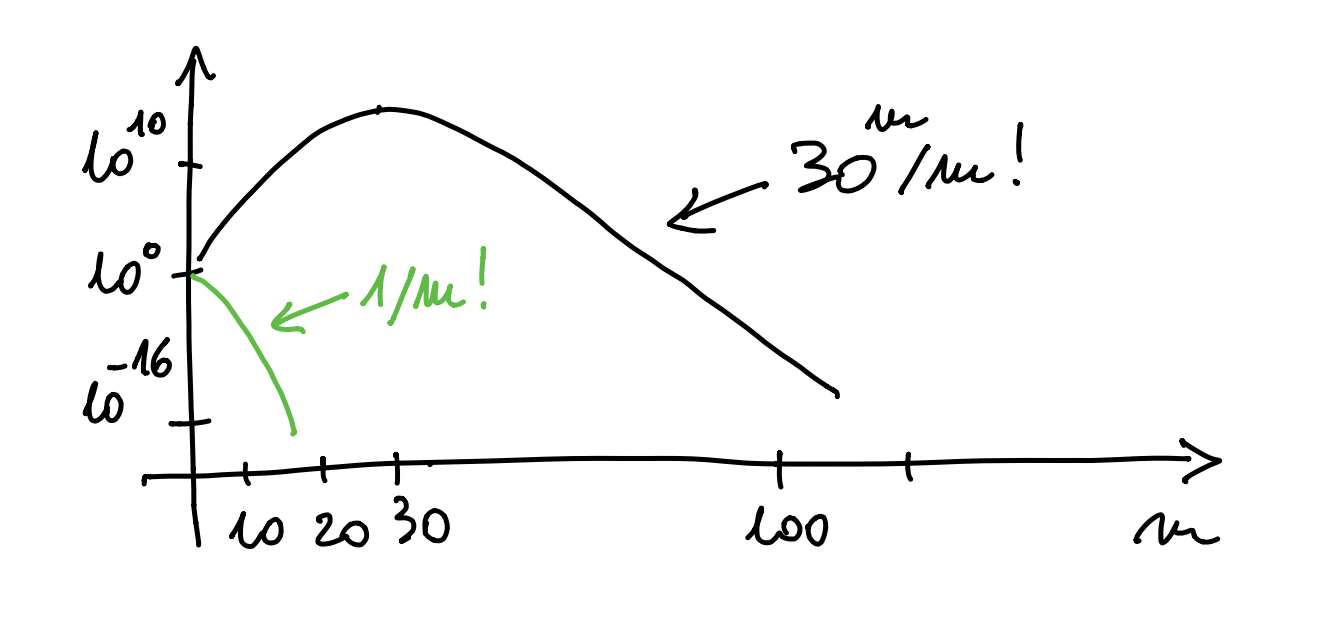
\includegraphics[width=0.5\textwidth]{foto/grafo1}
\end{center}
Di conseguenza il calcolo di $e^x$ alla precisione di macchina con la formula di Taylor è molto efficiente per $x \le 1$ ma richiede un polinomio di Taylor di grado $> [x]$ per $x>1$. \\
D'altra parte sfruttando le proprietà della funzione esponenziale si può adottare il seguente trucco
\[e^x = (e^{\frac{x}{n}})^n\]
dove si scala la variabile $x$ con $n \in \mathbb{N} , n > x$ (ad es. basta $n = [x]+1$), si approssima $e^y, y = \frac{x}{n}<1$, alla precisione di macchina con $t_{18}(y)$ e poi si calcola la potenza con l'algoritmo rapido basato sulla codifica binaria di $n$, a costo minore di $2[log_2(n)]$.\\
Si osservi anche che il calcolo di $t_{18} (y)$ è stabile, perché $y>0$ e tutte le operazioni coinvolte sono stabili (addizioni e moltiplicazioni con lo schema di Hörner, in tutto $18\cdot 2=36$ flops). \\
In definitiva con al massimo $36+2[ \log_2([x]+1)]$ flops abbiamo un algoritmo che calcola $e^x$ alla precisione di macchina (fino a $x \approx 708$ che è la soglia di overflow il costo è dell'ordine delle decine di flops).
Il Matlab adotta sostanzialmente questa tecnica per $exp$ (con una formula più accurata di quella di Taylor per $e^y$ con $0<y\le 1$ ).
\newpage

% ############# CAPITOLO 2 #####################
\chapter{Soluzione numerica di equazioni non lineari}
\section[Lezione 8 - Metodo di bisezione]{Lezione 8 - Introduzione alla soluzione numerica di equazioni non lineari, metodo di bisezione}
\subsection{Introduzione}
In questa e nelle prossime 3 lezioni ci occupiamo di un argomento classico del calcolo numerico, ovvero la soluzione numerica (cioè approssimata) di equazioni non lineari. Tratteremo 2 tipi di equazioni
\begin{itemize}
    \item $f(x)=0$, \uline{zeri} di funzione
    \item $x=\phi(x)$, equazioni di \uline{punto fisso}
\end{itemize}
che possiamo schematizzare coi seguenti disegni
\begin{center}
        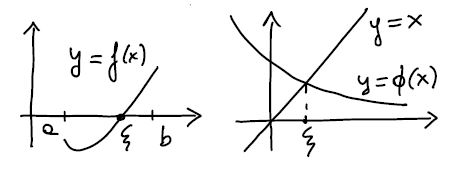
\includegraphics[width=0.5\textwidth]{foto/1}\par
\end{center}
Il primo tipo corrisponde al calcolo di uno zero di una funzione (continua), cioè di un punto $\xi$ in cui $f$ si annulla. Il secondo tipo corrisponde invece al calcolo del punto fisso $\xi$ di una funzione (continua) $\phi$ e si può interpretare come calcolo dell'ascissa dell'intersezione del grafico della bisettrice del primo e terzo quadrante $y=x$ col grafico di $y=\phi(x)$.\\ In entrambi i casi daremo \uline{condizioni sufficienti} per \uline{l'esistenza} ($\exists$) e l'unicità (!) della soluzione in un dato intervallo e discuteremo, analizzando in dettaglio, tre metodi classici di soluzione: i metodi di \uline{BISEZIONE} e di \uline{NEWTON} (tangenti) per gli zeri e il metodo delle \uline{ITERAZIONI DI PUNTO FISSO}.
\newline
Cominciamo col ricordare alcuni risultati di esistenza e unicità nel caso della ricerca di zeri.

\subsubsection{TEOREMA (degli zeri di funzioni continue)}
\begin{center}
    \fbox{\begin{minipage}[t]{15cm}%
        Sia $f(x)\in C[a,b]$ (cioè $f$ continua nell'intervallo chiuso e limitato $[a,b]$ e $f(a)f(b)<0$ cioè $f$ cambia segno agli estremi)
        allora 
        \begin{center}
        $\exists \xi\in(a,b):f(\xi)=0$
        \end{center}
    \end{minipage}}
\end{center}
Osserviamo che tale zero può non essere unico:
\begin{center}
    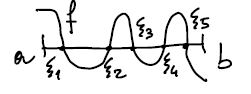
\includegraphics[width=0.3\textwidth]{foto/2}\par
\end{center}
D'altra parte togliendo una delle ipotesi la condizione restante \uline{non} basta a garantire l'$\exists$
\begin{center}
    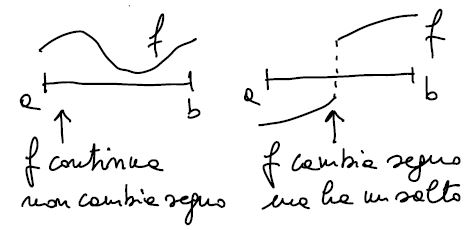
\includegraphics[width=0.5\textwidth]{foto/3}\par
\end{center}
Ribadiamo che le condizioni \uline{non} sono \uline{necessarie}
\begin{center}
    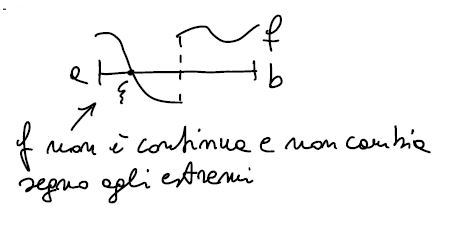
\includegraphics[width=0.5\textwidth]{foto/4}\par
\end{center}
Diamo anche due classiche condizioni \uline{sufficienti} ciascuna delle quali garantisce l'\uline{unicità} dello zero
\begin{itemize}
    \item $f$ \uline{strettamente monotona} (strettamente crescente o decrescente in $[a,b]$
    \item $f \in C[a,b]$, $f(a)f(b)<0$ e $f$ \uline{strettamente convessa} o \uline{concava} in $[a,b]$
\end{itemize}
Nel caso in cui $f$ è derivabile in $[a,b]$ la monotonia stretta è legata al segno di $f'$

\[\begin{split}
    f'(x)>0  \text{ in }  [a,b] & \Rightarrow f \text{ strettamente crescente } \\
    f'(x)<0  \text{ in }  [a,b] & \Rightarrow f \text{ strettamente decrescente }
\end{split}\]
Ricordiamo che il viceversa è vero con la diseguaglianza non stretta,
\[\begin{split}
    f \text{ strettamente crescente } & \Rightarrow f'(x)\ge 0 \text{ in } [a,b] \\
    f \text{ strettamente decrescente } & \Rightarrow f'(x)\le 0 \text{ in } [a,b] 
\end{split}\]
come si vede ad esempio con la funzione $f(x)=x^3$ in $[-1,1]$
\begin{center}
    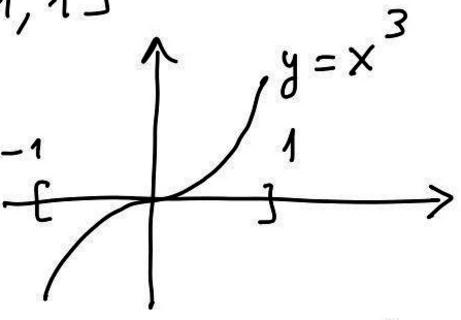
\includegraphics[width=0.3\textwidth]{foto/5}\par
\end{center}
Per cui si ha che $f$ è strettamente crescente ma $f'(0)=3x^2|_{x=0}=0$.\\
Analogamente convessità e concavità stretta sono legate al segno di $f''$ quando $f$ è derivabile 2 volte in $[a,b]$
\[\begin{split}
    f''(x)>0  \text{ in }  [a,b] & \Rightarrow f \text{ strettamente convessa } \\
    f''(x)<0  \text{ in }  [a,b] & \Rightarrow f \text{ strettamente concava }
\end{split}\]
Di nuovo, il viceversa è vero con la disuguaglianza non stretta
\[\begin{split}
    f \text{ strettamente convessa } & \Rightarrow f''(x)\ge 0 \text{ in } [a,b] \\
    f \text{ strettamente concava } & \Rightarrow f''(x)\le 0 \text{ in } [a,b] 
\end{split}\]
($f(x) = x^4$ è  strettamente convessa in $[-1,1]$, $f''(0) = 0$)

Ribadiamo che le condizioni di unicità date sono solo sufficienti 
\begin{center}
    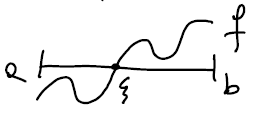
\includegraphics[width=0.3\textwidth]{foto/pagina8_1}\par
$\uparrow$ \\
non è ne monotona ne convessa o concava ma $\xi$ è unico\\
\end{center}
Fatti questi brevi richiami teorici su $\exists!$ delle soluzioni di equazioni scritte nella forma 
\[f(x)=0, \quad x \in [a,b]\]
introduciamo uno dei metodi più semplici per la soluzione numerica, il \textbf{metodo} \textbf{di} \textbf{bisezione}.

\subsection{Metodo di bisezione}
Il metodo di bisezione consiste nell'applicazione iterativa del teorema degli zeri di funzioni continue, quindi si assume che 
\[f \in C[a,b], \quad f(a)f(b)<0\]
Illustriamo graficamente la costruzione delle iterazioni
\begin{center}
            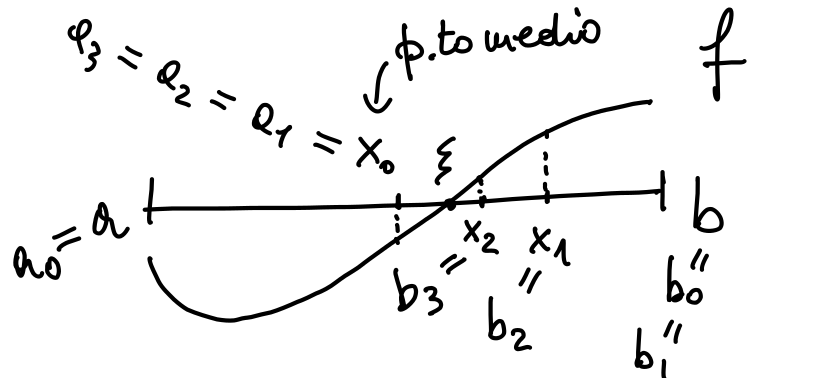
\includegraphics[width=0.5\textwidth]{foto/im_pag10}\par
\end{center}
L'idea è la seguente: si parte da $[a_0,b_0]=[a,b]$, si calcola il punto medio $x_0=\frac{(a_0+b_0)}{2}$; ora se $f(x_0)=0$ siamo su uno zero; altrimenti siccome $f(a_0)$ e $f(b_0)$ hanno segno definito, $f(x_0)$ sarà discorde con uno solo dei due e quindi sicuramente ci sarà uno zero in $(a_0,x_0)$ se $f(a_0)f(x_0)<0$ altrimenti ci sarà uno zero in $(x_0, b_0)$ visto che $f(x_0)f(b_0)<0$ (sempre per il teorema degli zeri). Nel primo caso si definisce $a_1=a_0$, $b_1=x_0$, mentre nel secondo $a_1=x_0$, $b_1=b_0$, con la garanzia che $\exists \ \xi \in (a_1,b_1)$ tale che $f(\xi)=0$ visto che $f(a_1)f(b_1)<0$.

\subsubsection{Convergenza}
Il procedimento viene iterato applicando ripetutamente il teorema degli zeri per passare da $[a_n,b_n]$ ad $[a_{n+1},b_{n+1}]$ in cui uno degli estremi è diventato il punto medio $x_n=\frac{(a_n+b_n)}{2}$ di $[a_n,b_n]$.\\
Si tratta in generale di un processo infinito (a meno che per qualche $n$ non risulti $f(x_n)=0$) che permette di costruire 3 successioni $\{ a_n \} , \{ b_n \} , \{ x_n \} $ tali che:
\begin{itemize}
    \item $\exists\ \xi : f(\xi)=0, \ \xi \in (a_n,b_n)$
    \item $\abs{\,\xi - a_n\,}, \ \abs{\,\xi - b_n\,} \le b_n-a_n=\frac{b-a}{2^n}$
    \item $\abs{\,\xi - x_n\,} < \frac{b_n - a_n}{2} = \frac{b-a}{2^{n+1}}$
\end{itemize}
$n=0,1,2,\dots$ \\
Il nome ``bisezione" viene dal fatto che l'intervallo viene diviso iterativamente a metà, ``buttando via" ad ogni iterazione mezzo intervallo per restare nella metà dove $f$ cambia segno e dove quindi c'è sicuramente uno zero (``lo" zero nel caso questo sia unico in $(a,b)$, ma in generale il metodo funziona anche con vari zeri, calcolandone uno). \\
Si vede subito che il metodo è convergente, cioè che tutte e 3 le successioni convergono ad uno zero $\xi \in (a,b)$.\\
Infatti
\[0 \le \abs{\,\xi - a_n\,}, \ \abs{\,\xi - b_n\,} < \frac{b-a}{2^n}\underset{n\to \infty}{\longrightarrow}  0\]
e per il teorema dei 2 carabinieri
\[\abs{\,\xi - a_n\,}, \ \abs{\,\xi - b_n\,} \longrightarrow 0, \ n \rightarrow \infty\]
analogamente
\[\abs{\,\xi - x_n\,} \longrightarrow 0, \ n \rightarrow \infty\]
visto che 
\[0 \le \abs{\,\xi - x_n\,} < \frac{b-a}{2^{n+1}}\]
Quest'ultima diseguaglianza è immediatamente comprensibile da questo disegno
\begin{center}
    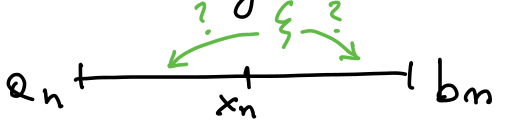
\includegraphics[width=0.5\textwidth]{foto/6}\par
\end{center}
Cioè sappiamo che $\xi$ zero di $f$ sta in $(a_n, b_n)$, non sappiamo dove, ma sicuramente la sua distanza dal punto medio $x_n$ è minore di metà della lunghezza dell'intervallo $[a_n, b_n]$ cioè è $< \frac{(b_n - a_n)}{2}$, in altri termini, $\xi$ sta nell'intorno aperto di centro $x_n$ e raggio $\frac{(b_n - a_n)}{2}$. \\
Nel metodo di bisezione si sceglie $x_n$ come successione di approssimazioni, visto che la \uline{stima} dell'errore è migliore di un fattore $\frac{1}{2}$ rispetto a quella di $a_n$ e $b_n$.

\subsubsection{Stima a priori}
Volendo garantire una tolleranza di $\varepsilon > 0 $ nel calcolo approssimato del vero $\xi$, basta quindi risolvere la disuguaglianza di 
\[ e_n = \abs{\,\xi - x_n\,} < \frac{b-a}{2^{n+1}} \le \varepsilon \]
in modo che $\xi \in (x_n -  \varepsilon, x_n + \varepsilon)$, ovvero \[ 2^{n+1} \geq  \frac{b-a}{\varepsilon} \]
cioè
\[\begin{split}
   n + 1 & \ge \log_2{\frac{b-a}{\varepsilon}} \\
    & = log_2\left(b-a\right) + log_2\left(\frac{1}{\varepsilon}\right)
\end{split}\]
Questa disuguaglianza permette ``a priori", cioè prima di iniziare il processo di calcolo, di decidere a quale iterazione fermarsi in modo da garantire la tolleranza di $\varepsilon > 0$, basta prendere 
\[ n(\varepsilon) = [\log_2\left(\frac{1}{\varepsilon}\right) + log_2{(b-a)}] \quad \leftarrow \text{parte intera}\]
In effetti una stima del tipo $e_n \leq stima(n)$ dove la stima non dipende dalle quantità calcolate si chiama usualmente ``STIMA A PRIORI".\\
Il problema con le stime a priori è che sono spesso SOVRASTIME, cioè non sono vicine all'errore effettivo ma ne danno solo un confine superiore garantito in modo teorico, che però può portare ad un aumento del numero di iterazioni e quindi del costo computazionale, rispetto a quello che sarebbe sufficiente ad ottenere la tolleranza richiesta.

\subsubsection{Stima a posteriori - residuo pesato}
Per ottenere una stima dell'errore più aderente, cominciamo col fare la seguente osservazione: visto che $x_n \to \xi,\,n\to \infty$ e che $f$ è continua, si avrà che \[f(x_n) \to f(\xi)=0,\quad n \to \infty\]
Quella che stiamo usando qui in realtà è una caratterizzazione della continuità di una funzione in analisi matematica: $f$ è continua in $l$ \uline{se e solo se}
\[\forall \{x_n\}:\lim_{n\to \infty}x_n=l \text{ si ha} \lim_{n\to \infty}f(x_n)=f(l)\]
che si esprime anche dicendo ``$f$ è continua se e solo se il limite si può trasportare 'dentro' la funzione".\\
Nel nostro caso $f(\xi)=0$ quindi $f(x_n) \to 0,\,n \to \infty$ e anche $\abs{\,f(x_n)\,}\to 0,\,n \to \infty$.\\
La quantità $\abs{\,f(x_n)\,}$ si chiama ``RESIDUO" perchè dice quanto ``resta" ad $f$ per annullarsi.\\
Viene allora spontanea questa domanda: siccome $f(x_n) \to 0,\,n \to \infty$, possiamo arrestare il processo di calcolo quando il residuo $\abs{\,f(x_n)\,}$ è piccolo? In altre parole
\[\abs{\,f(x_n)\,}\le \varepsilon \overset{?}{\Longrightarrow} e_n \le \varepsilon\]
La risposta è \uline{NO}, in realtà\\
\[\abs{\,f(x_n)\,}\le \varepsilon \nRightarrow e_n\le \varepsilon\]
perchè come vedremo subito la grandezza del residuo non è in se' un buon indicatore dell'errore, ma va opportunamente ``pesata": per capirlo consideriamo i seguenti grafici\\
\begin{center}
    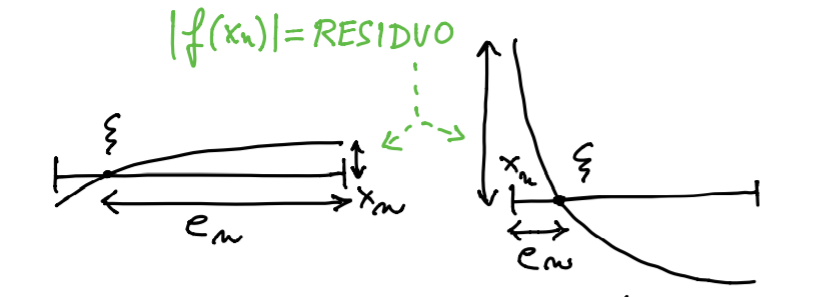
\includegraphics[width=0.6\textwidth]{foto/grafo4}
\end{center}
Nel primo caso il residuo è piccolo ma l'errore è grande (cioè il residuo è una \uline{SOTTOSTIMA} dell'errore).\\
Nel secondo caso il residuo è grande ma l'errore è piccolo (cioè il residuo è una \uline{SOVRASTIMA} dell'errore).\\
È importante osservare che una \uline{sottostima} dell'errore in pratica è la cosa più \uline{pericolosa}, perchè induce a fermare le iterazioni quando $x_{n}$ non è ancora nell'intorno del limite individuato dalla tolleranza: si pensa di aver approssimato la quantità limite a meno della tolleranza e invece \uline{l'errore è più grande della tolleranza}.\\
Questo può chiaramente portare a conseguenze gravi in applicazioni in cui il rispetto della tolleranza è decisivo.
D'altra parte, una \uline{sovrastima} pur essendo meno grave, ha come conseguenza un aumento del numero di iterazioni rispetto a quello che sarebbe sufficiente e quindi un \uline{incremento} del \uline{costo computazionale}.\\
Nei due grafici disegnati sopra si nota che il residuo è una sottostima dell'errore quando la funzione è ``piatta", cioè la variazione è lenta in un intorno dello zero, mentre è una sovrastima quando la funzione è ``ripida", cioè ha una variazione veloce in un intorno dello zero.
Si capisce allora che il residuo va in qualche modo ``pesato" per tener conto della velocità di variazione: se $f$ è derivabile, bisogna quindi tenere conto della grandezza della derivata, che per definizione misura la velocità di variazione di una funzione per fare questo in modo rigoroso possiamo ricorrere a un teorema chiave del calcolo differenziale, il teorema del VALOR MEDIO (detto anche teorema di Lagrange).

\subsubsection{TEOREMA (del valor medio)}
\begin{center}
    \fbox{\begin{minipage}[t]{15cm}%
        Sia $f \in C[\alpha,\beta]$ derivabile in $(\alpha,\beta)$
        allora 
        \begin{center}
        $\exists\, z\in (\alpha,\beta)$ tale che $\frac{f(\beta) - f(\alpha)}{\beta - \alpha} = f'(z)$
        \end{center}
    \end{minipage}}
\end{center}
Interpretazione geometrica
\begin{center}
   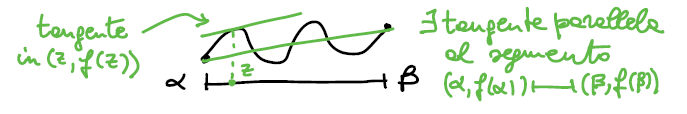
\includegraphics{foto/pag25} 
\end{center}
Tornando all'analisi del residuo nel metodo di bisezione, mettiamoci nelle seguenti ipotesi: $f\in C^1[a,b]$ (cioè $f$ è derivabile con derivata prima continua in $[a,b]$), $\{x_n\}\subset[c,d]\subseteq[a,b]$ (almeno per $n\ge n_0$ cioè per $n$ abbastanza grande) con \[x_n \to \xi,\,n \to \infty,\,f(\xi)=0 \text{ e } f'(x)\ne 0\quad \forall x\in [c,d]\] allora vale la rappresentazione:
\[e_n = \abs{\,x_n-\xi\,} = \frac{\abs{\,f(x_n)\,}}{\abs{\,f'(z_n)\,}},\quad n\ge n_0\] con $z_n\in int(x_n,\xi)$, l'intervallo aperto che ha per estremi $x_n$ e $\xi$ (potrebbe essere $(x_n,\xi)$ oppure $(\xi,x_n)$ a seconda che $x_n<\xi$ oppure $x_n>\xi$).
\newline \newline
Prima di dimostrare la stima, osserviamo che
\begin{enumerate}
    \item la rappresentazione dell'errore mostra chiaramente che l'\uline{ERRORE} è un \uline{RESIDUO PESATO} della derivata;
    \item l'ipotesi che $f'(x)\ne0$ in $[c,d]\subseteq [a,b]$ è equivalente all'ipotesi che lo zero sia SEMPLICE, ovvero che $f'(\xi)\ne 0$ (la terminologia viene dalle equazioni algebriche, cioè quelle in cui $f$ è un polinomio, lì zero semplice significa che $(x-\xi)^{\alpha}$ compare con $\alpha =1$ nella fattorizzazione di Ruffini). Infatti, se $x_n\in [c,d]\quad \forall n>n_0$ allora $\xi=\lim x_n\in [c,d]$ perchè $[c,d]$ è chiuso e quindi contiene i limiti delle successioni lì contenute, quindi $f'(\xi)\ne 0$.
    Viceversa, se $f'(\xi)\ne 0$ siccome $f'$ è continua, per il teorema della \uline{permanenza del segno}
    \[\exists\, \delta>0 : f'(x)\ne 0\quad \forall x \in [\xi - \delta, \xi + \delta] = [c,d]\]
    e siccome $x_n \to \xi,\,n \to \infty\quad \exists \,n_0$ tale che $|x_n-\xi|\le \delta \quad \forall n \ge n_0$\\
    Si noti che $f'(z_n)\ne 0,\, n\ge n_0$ perchè $z_n \in int(x_n,\xi)\subset[c,d]$.\\
    È importante osservare che la rappresentazione dell'errore come residuo pesato non vale solo per il metodo di bisezione, ma per ogni metodo convergente a uno zero semplice se $f\in C^1$ (applicheremo infatti questo risultato più avanti al metodo di Newton)
    \item dalla rappresentazione siamo in grado di ricavare delle STIME A POSTERIORI dell'errore (a posteriori perchè si utilizza il residuo che è calcolabile solo a posteriori dopo aver prodotto $x_n$ nel processo di calcolo)
\end{enumerate}
\begin{proof}[\unskip\nopunct]
\uline{DIMOSTRAZIONE} della rappresentazione utilizzando il teorema del valor medio e supponendo che $x_n>\xi$ (l'altro caso è del tutto analogo), con $\alpha=\xi, \beta=x_n$
\[ f(x_n)-f(\xi) = f'(z_n)(x_n-\xi), \text{ } z_n \in (\xi,x_n)\]
con $f(\xi)=0$, cioè
\[ \abs{\,f(x_n)\,} = \abs{\,f'(z_n)\,}\abs{\,x_n-\xi\,} \]
che si può riscrivere come
\[ e_n = \abs{\,x_n-\xi\,} = \frac{\abs{\,f(x_n)\,}}{\abs{\,f'(z_n)\,}} \]
\end{proof}

Ora, siccome il teorema del valor medio non dice chi sia $z_n$ ma solo che esiste almeno un $z_n$ in $int(x_n,\xi)$, cerchiamo di ricavare delle stime ``pratiche" dell'errore utilizzando il residuo opportunamente pesato.

\begin{enumerate}[label=\roman*)]
\item Se è noto che $\abs{\,f'(x)\,} \ge k >0$ $\forall x \in [a,b]$ (ma basta $\forall x \in [c,d]$), allora
\[e_n = \frac{\abs{\,f(x_n)\,}}{\abs{\,f'(z_n)\,}} \underset{\underset{\underset{rigorosa}{stima}}{\uparrow}}{\le} \frac{|f(x_n)|}{k} \]

\item Se $f'$ è nota o calcolabile, siccome $z_n \to \xi, n \to \infty$ per il teorema dei 2 carabinieri visto che $z_n$ sta fra $\xi$ e $x_n$, per la continuità di $f'$ si ha che
\[ \abs{\,f'(x_n)\,}, \, \abs{\,f'(z_n)\,} \underset{n \to \infty}{\longrightarrow} \abs{\,f'(\xi)\,} \ne 0 \]
Quindi, almeno per $n$ abbastanza grande, $\abs{\,f'(x_n)\,}$ e $\abs{\,f'(z_n)\,}$  saranno entrambi dell'ordine di grandezza di $\abs{\,f'(\xi)\,}$ (notiamo che nel residuo pesato quello che interessa è essenzialmente \uline{l'ordine di grandezza del} \uline{peso} $\abs{\,f'(z_n)\,}$: per fissare le idee, sto dividendo per $100$ o per $\frac{1}{100}$? Cioè, sto ``aggiustando" una sovrastima o una sottostima?).\\
Abbiamo quindi una ``STIMA EMPIRICA":
\[ e_n = \abs{\,x_n-\xi\,} \approx \frac{\abs{\,f(x_n)\,}}{\abs{\,f'(x_n)\,}} \] 
valida almeno per $n \ge \bar{n}$, dove $\bar{n}$ corrisponde ad un controllo empirico che l'ordine di grandezza di $\abs{\,f'(x_n)\,}$ si stia ``stabilizzando", cioè valga:
\[ \abs*{\,\frac{\abs{\,f'(x_n)\,}}{\abs{\,f'(x_{n-1})\,}}-1\,} \le \delta \]


Ad esempio con $\delta = 10^{-1}$ o $10^{-2}$ $\left(\frac{\abs{\,f'(x_n)\,}}{\abs{\,f'(x_{n-1})\,}} \to 1,\ n \to \infty \right)$, quindi ha senso controllare quando il rapporto si sta stabilizzando intorno a $1$, tenendo presente che questo è un criterio sensato ma non completamente rigoroso, diciamo una ``linea guida" per l'utilizzo del peso.

\item Se $f'$ non è vuota esplicitamente, va in qualche modo approssimata.\\Osserviamo infatti che non sempre abbiamo a disposizione una formula analitica per $f$ (come ad es. per l'equazione algebrica $x^2-2=0$ corrispondente al calcolo di $\sqrt{2}$ o per l'equazione non algebrica $x-e^{-x}=0$)\\
Infatti $f$ potrebbe essere nota in forma di ``scatola nera"\\
\begin{center}
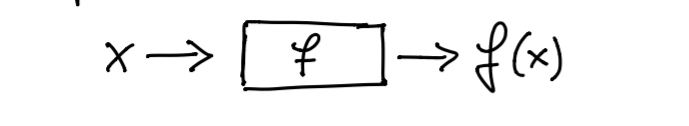
\includegraphics[width=0.5\textwidth]{foto/scatolanera}    
\end{center}
cioè potremmo avere a disposizione solo i valori da misure o da altri algoritmi. Se però sappiamo almeno che $f$ è derivabile, possiamo approssimare $f'$ con un rapporto incrementale costruito con le quantità calcolate 
\[f'(z_n)\approx \vartheta_n=\frac{f(x_n)-f(x_{n-1})}{x_n-x_{n-1}}\overset{\overset{\overset{VALOR}{MEDIO}}{\downarrow}}{=} f'(\mu_n)\]
dove $int(x_n,x_{n-1})\ni \mu_n \rightarrow \xi, n\rightarrow\infty$ e quindi 
\[\abs{\,\vartheta_n\,}\approx \abs{\,f'(\xi)\,} \approx\abs{\,f'(z_n)\,}\] almeno per $n$ abbastanza grande: di nuovo, possiamo usare un criterio empirico per ``accettare" il valore di $\abs{\,\vartheta_n\,}$ come peso, tipo $\abs*{\,\frac{\abs{\,\vartheta_n\,}}{\abs{\,\vartheta_{n-1}\,}}-1\,}\le \delta$ 

Detto $k_n$ il peso calcolato con uno degli approcci $(i)-(iii)$, siamo allora in grado di scrivere un ``\uline{test di arresto}" per il metodo di bisezione che \uline{combina} stima \uline{a priori} e stima \uline{a posteriori}
\[min\left\{\frac{b-a}{2^{n+1}},\frac{\abs{\,f(x_n)}\,}{k_n}\right\}\le \varepsilon\]
\end{enumerate}
Possiamo a questo punto fare alcune considerazioni di carattere computazionale.

\begin{enumerate}[label=\Alph*)]
\item il metodo di bisezione funziona con \uline{richieste} analitiche e computazionali \uline{minime}.
La versione base con la stima a priori chiede solo che siano soddisfatte le ipotesi del teorema degli zeri (continuità e cambio segno agli estremi) e unicamente la possibilità di calcolare correttamente il segno di $f(x_n)$ (per cui è sufficiente un errore relativo $<100\%$ su $f(x_n)!$). Infatti in generale se 
\[\tilde{\alpha} \approx \alpha \ne 0 \quad \text{e} \quad \frac{\abs{\,\alpha-\tilde{\alpha}\,}}{\abs{\,\alpha\,}}<1 \quad \Longrightarrow \quad sign(\tilde{\alpha})=sign(\alpha)\]

\item mentre la stima a priori è decrescente, l'errore effettivo in generale non lo è, come si vede da questo disegno
\begin{center}
    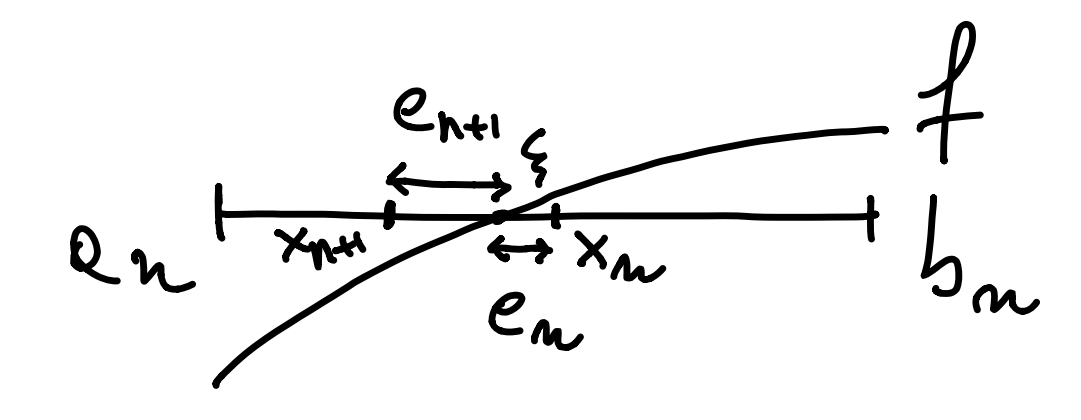
\includegraphics[width=0.5\textwidth]{foto/grafo3}\par
\end{center}
 dove $e_{n+1}>e_n$ ( anche se comunque $e_n \rightarrow 0, n \rightarrow \infty$); qui si vede anche che $e_n\ll\frac{(b_n-a_n)}{2}$ e la stima del residuo pesato è tendenzialmente più accurata. A differenza della stima a priori che si dimezza, $e_{n+1}\approx\frac{e_n}{2}$ solo ``in media" su un po' di iterazioni.
\end{enumerate}

Concludiamo la lezione con un esempio, il calcolo approssimato di $\sqrt{2}$ risolvendo l'equazione algebrica $x^2 -2 = 0$ con il metodo di bisezione.\newline

\subsubsection{Calcolo di $\sqrt{2}$ alla precisione di macchina}
Consideriamo l'equazione algebrica
\[f(x)=x^2-2=0\] Calcolarne la soluzione positiva significa calcolare $\sqrt{2}$. Le ipotesi del teorema degli zeri sono soddisfatte in $[a,b]=[1,2]$.\\
Infatti $f\in C[a,b]$ (anzi $f\in C^{\infty}(\mathbb{R})$ cioè è derivabile infinite volte in $\mathbb{R}$ con derivate tutte continue, perché $f$ è un polinomio) \[f(a)=f(1)=1-2=-1<0\] \[f(b)=f(2)=2^2-2=2>0\]
Inoltre $f'(x)=2x \geq 2\quad\forall x \in [1,2]$ quindi $\sqrt{2}\in (1,2)$ ed è l'unico zero in tale intervallo (in effetti sappiamo che è l'unico zero in $\mathbb{R}^+$)
possiamo applicare il metodo di bisezione che comincia in questo modo: 
\[\begin{split}
    x_0 & = \frac{1+2}{2} = 1.5, \\
    x_1 & = \frac{1+1.5}{2} = 1.25, \\
    x_2 & = \frac{1.25+1.5}{2} = \frac{2.75}{2} = 1.375, \\
    x_3 & = \frac{1.375+1.5}{2} = 1.4375, \\
    \dotso
\end{split}\]
(ricordiamo che $\sqrt{2}=1.4142\dots$).\\
Nel grafico sottostante (in scala log) riportiamo l'errore effettivo, la stima a priori \[\frac{(b_n-a_n)}{2}=\frac{1}{2^{n+1}}\] 
e la stima a posteriori
\[\frac{\abs{\,f(x_n)\,}}{k}=\frac{\abs{\,x_n^2-2\,}}{2}\]
(visto che $f'(x)\ge k=2 \quad \forall x\in [1,2]$) tutte relativizzate a $\abs{\,\xi\,}=\sqrt{2}$ (in questo caso comunque $\abs{\,\xi\,}$ è dell'ordine dell'unità e quindi errore assoluto e relativo vicini)
\begin{center}
    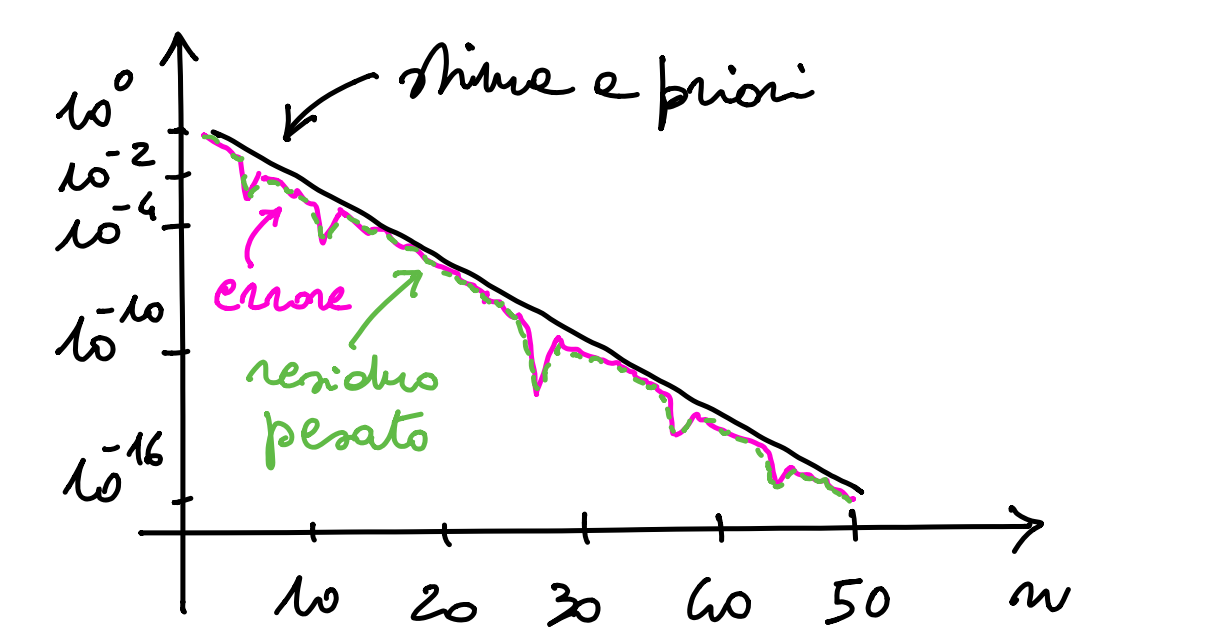
\includegraphics[width=0.5\textwidth]{foto/grafo2}\par
\end{center}
(come sempre per comodità i valori discreti sono interpolati con linee continue o tratteggiate).\\
Si vede che l'errore segue solo ``in media" l'andamento della stima a priori, che la sovrastima a volte di vari ordini di grandezza (picchi dell'errore verso il basso, ad esempio tra $n=20$ e $n=30$ l'errore va circa a $10^{-11}$ mentre la stima a priori ha bisogno di una decina di iterazioni in più).\\
D'altra parte la stima del residuo pesato è praticamente sovrapposta all'errore effettivo.\\
Si noti infine che per raggiungere un errore dell'ordine della precisione di macchina $\varepsilon_M=2^{-53}$ servono circa $50$ iterazioni, il che non è sorprendente visto che il fattore medio di riduzione dell'errore è $\frac{1}{2}$.
\newpage

\section[Lezione 9 - Metodo di Newton]{Lezione 9 - Metodo di Newton (tangenti), convergenza e velocità di convergenza}
\subsection{Velocità di convergenza metodo di bisezione}
Come abbiamo visto nella scorsa lezione, il metodo di bisezione è un metodo semplice ed efficace per la soluzione numerica di equazioni non lineari, in grado di funzionare con richieste minimali, sia dal punto di vista analitico (ipotesi del teorema degli zeri delle funzioni continue) sia computazionali (basta saper calcolare il segno di $f(x_n)$ cioè fare su $f(x_n)$ un errore relativo $<100\%$).\\
Accanto a questi indubbi vantaggi, il metodo di bisezione ha però un handicap: è abbastanza ``lento". Come abbiamo visto, la stima a priori dell'errore decade di un fattore $\frac{1}{2}$ ad ogni iterazione e l'errore lo fa ``in media", cioè 
\[ e_{n+1} \approx \frac{1}{2} \cdot e_n \]
non esattamente ad ogni iterazione ma in media su un certo numero di iterazioni.\\
Ovviamente la stessa proprietà vale in media per l'errore relativo
\[ r_{n+1}=\frac{e_{n+1}}{\abs{\,\xi\,}} \approx \frac{1}{2} \cdot \frac{e_n}{\abs{\,\xi\,}} = \frac{1}{2} \cdot r_n \]
per $\xi \ne 0$; sono quindi necessarie in media $3-4$ iterazioni affinché l'errore relativo scenda di $\frac{1}{10}$ (cioè per guadagnare una cifra decimale corretta), visto che 
\[\frac{1}{16} = \left(\frac{1}{2}\right)^4 < \frac{1}{10} < \left(\frac{1}{2}\right)^3 = \frac{1}{8}\] 
(infatti abbiamo visto che per calcolare $\sqrt{2}$ alla precisione di macchina in Matlab servono una cinquantina di iterazioni e in effetti $\varepsilon_M = 2^{-53} \approx 10^{-16}$).

\subsection{Metodo di Newton}
In queste lezioni introdurremo un metodo molto più efficiente per il calcolo di zeri, ovvero il metodo di \uline{Newton}, o metodo delle \uline{tangenti}, che come si capisce dal nome risale agli albori del calcolo differenziale nel XVII secolo.\\
La maggior efficienza avrà un prezzo in termini di richieste analitiche ($f$ almeno derivabile in $[a, b]$) e computazionali (saper calcolare sia $f$ che $f'$ con buona accuratezza).\\
L'idea del metodo è semplice: si tratta di \uline{LINEARIZZARE} iterativamente l'equazione $f(x) = 0$ sostituendo $f$ ad ogni iterazione con la retta tangente nel punto ($x_n, f(x_n)$) del grafico (purché $f$ sia derivabile), come vediamo nel disegno qui sotto 
\begin{center}
    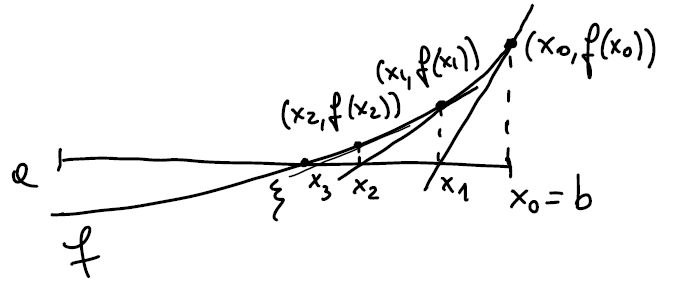
\includegraphics[scale=0.7]{foto/pagina5_1}
\end{center}
Per trovare l'espressione analitica delle iterazioni, calcoliamo lo zero della retta tangente nel punto($x_0,f(x_0)$):
\[ \begin{cases}
    y = 0 & \text{asse } x\\
    y = f(x_0) + f'(x_0)(x-x_0) & \text{retta tangente}
\end{cases}\]
dove stiamo usando l'interpretazione geometrica della derivata nel punto $x_0$ come coefficiente angolare della retta tangente nel corrispondente punto del grafico di $f$. Otteniamo l'equazione 
\[ 0=f(x_0)+ f'(x_0)(x-x_0) \]
la cui soluzione è
\[ x_1=x_0-\frac{f(x_0)}{f'(x_0)}, \quad f'(x_0)\neq 0 \]
Osserviamo subito che se $f'(x_0)=0$ la retta tangente sarebbe parallela all'asse $x$ e non avrebbe un punto di intersezione con esso; ma è essenziale anche la posizione del valore iniziale $x_0$, se scelto ``male" già la prima iterazione potrebbe far uscire dall'intervallo di definizione:\\
\begin{center}
    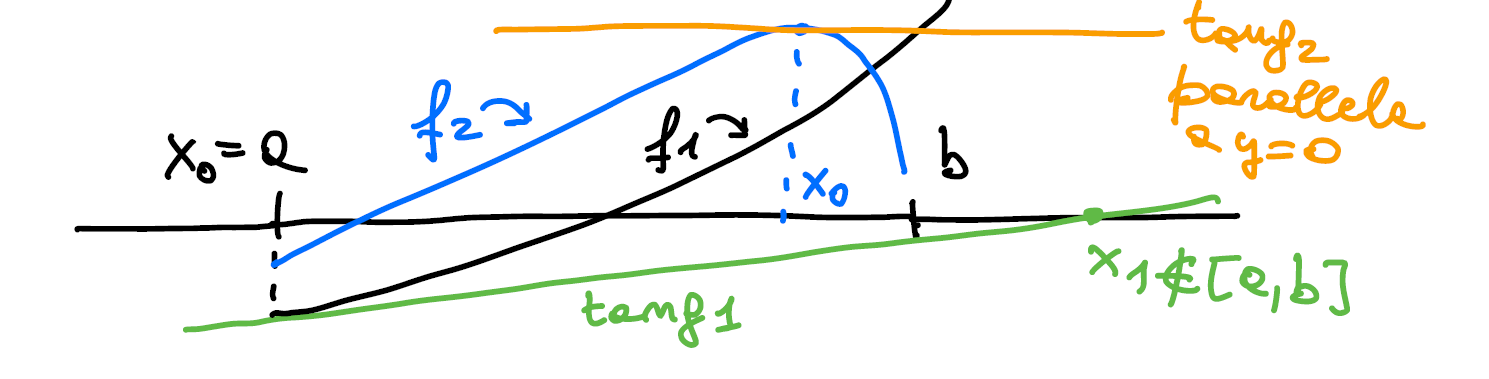
\includegraphics[scale=0.5]{foto/pagina7}
\end{center}
In generale, per ottenere $x_{n+1}$ a partire da $x_n$ (se $f'(x_n)\neq 0$) si cerca l'intersezione della tangente in ($x_n,f(x_n)$ con l'asse $x$ ($y=0$)\\
\[ \begin{cases}
        y=0\\
        y=f(x_n)+f'(x_n)(x-x_n)
\end{cases} \]
ottenendo la formula iterativa\\
\[ x_{n+1}=x_n-\frac{f(x_n)}{f'(x_n)}, \quad n=0,1,2,\dotso \]
Ora, come per tutti i metodi che producano una successione, cerchiamo delle condizioni che garantiscano la CONVERGENZA (in questo caso il limite dovrà essere lo zero $\xi$ di $f$).\\
Ci sono vari set di condizioni SUFFICIENTI che garantiscono la convergenza del metodo di Newton; ne mostriamo uno che assume, oltre alle ipotesi del teorema degli zeri, la derivabilità (essenziale perché la curva del grafico ammetta tangente in ogni punto) e la convessità o concavità stretta (tramite il segno di $f''$).

\subsubsection{TEOREMA (convergenza del metodo di Newton con $f''$ segno costante)}
\begin{center}
    \fbox{\begin{minipage}[t]{15cm}%
            Sia $f \in C^2[a,b]$ (derivabile 2 volte con derivate continue in $[a,b]$), $f(a)f(b)<0$, $f''(x)>0 \quad \forall x \in [a,b]$ (oppure $f''(x)<0 \quad \forall x \in [a,b]$), $x_0$ tali che $f(x_0)f''(x_0)>0$
        allora 
        \begin{center}
        il metodo di Newton è ben definito (cioè $f'(x_n) \neq 0 \ \ \forall n$)\\
        e converge all'unico zero $\xi$ di $f$ in $(a,b)$
        \end{center}
    \end{minipage}}
\end{center}
\begin{proof}[\unskip\nopunct]
\textbf{Dimostrazione}\\
Ci sono 4 casi possibili in base al segno di $f''$ ovvero
\begin{center}
    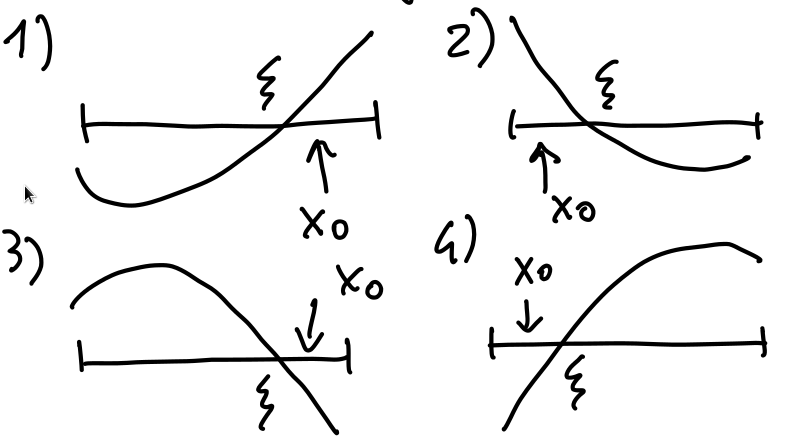
\includegraphics[scale=0.4]{foto/pagina11_1}
\end{center}
\begin{itemize}
    \item in (1) e (2) $f$ è strettamente convessa,
    \item in (3) e (4) concava,
    \item in (1) e (3) $x_0$ va scelto in $(\xi,b]$,
    \item in (2) e (4) $x_0 $ va scelto in $[a,\xi)$.
\end{itemize}
Vediamo dai disegni che non è escluso che $f'$ possa cambiare segno, l'ipotesi chiave è che non cambi segno $f''$; ovviamente sono compresi i casi in cui $f''$ non cambia segno e anche $f'$ non lo fa, ad esempio $f''(x) > 0$ e $f'(x) > 0 \quad \forall x \in [a,b]$, cioè $f$ è strettamente convessa e strettamente crescente in [a,b], tipo\\
\begin{center}
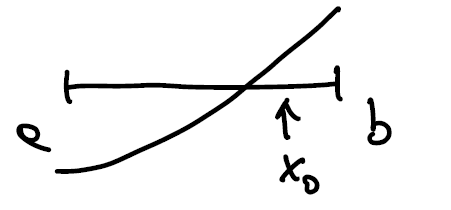
\includegraphics[width=0.3\textwidth]{foto/pagina12_1}
\end{center}
Per semplicità trattiamo il caso (1) perché negli altri casi la dimostrazione è analoga. \\
Siamo quindi in questa situazione\\
\begin{center}
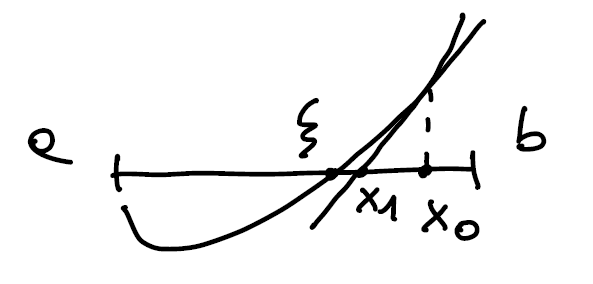
\includegraphics[width=0.3\textwidth]{foto/pagina12_2}
\end{center}
con $f(a) < 0$, $f(b) > 0$, $f''(x) > 0$, $\forall x \in [a,b]$, $x_0 \in (\xi,b]$\\
La dimostrazione si fa per induzione, mostrando che se $x_n \in (\xi, b]$ anche $x_{n+1} \in (\xi, b]$ e inoltre $x_{n+1} < x_n$ \\
Infatti \[x_{n+1} = x_n - \frac{f(x_n)}{f'(x_n)}\]
Ma se $x_n \in (\xi, b]$ allora $f'(x_n) > 0$ e $f(x_n) > 0$, quindi $x_{n+1}$ si ottiene da $x_n$ sottraendo una quantità $> 0$, cioè $x_{n+1} < x_n$.\\
D'altra parte f è strettamente convessa, il che è equivalente a dire che la tangente sta ``sotto al grafico" $\forall x \in [a,b]$.\\ 
Ma allora la tangente in un punto $\in (\xi, b]$ interseca l'asse $x$ a destra di $\xi$, cioè se $x_n \in (\xi, b]$ anche $x_{n+1} \in (\xi, b]$.\\
In definitiva, abbiamo provato che la successione $\{x_n\}$ è decrescente e che $x_n > \xi$ $\forall n$\\
Dall'analisi matematica è noto che una successione monotona e limitata ha limite e che il limite è $sup\{x_n\}$ se è crescente e $inf\{x_n\}$ se è decrescente (che corrisponde al nostro caso). \\
Quindi 
\[\exists \lim_{n \to \infty} x_n = inf\{x_n\} = \eta \quad \text{con} \quad \eta \geq \xi\]
Ricordiamo infatti che le disuguaglianze conservano il verso passando al limite oppure facendo $sup$ e $inf$ (le disgiunzioni strette possono diventare non strette, ma nello stesso verso:
\[ \begin{split}
	& x_n \geq \alpha \Rightarrow \lim, \inf, \sup \,x_n \geq \alpha \\ 
	& x_n > \alpha \Rightarrow \lim, \inf, \sup \,x_n \geq \alpha
\end{split} \]
come si dimostra facilmente con le proprietà del limite e di $sup$ e $inf$).\\
Per concludere la dimostrazione basta passare al limite della formula che definisce il metodo (per brevità scriveremo lim per $ \lim_{n \to \infty} $)
\[ \begin{split}
	\eta & = \lim x_{n+1} \\
	& = \lim \left( x_n - \frac{f(x_n)}{f'(x_n)} \right) \\
	& = \lim x_n - \lim\frac{f(x_n)}{f'(x_n)} \\
	& = \lim x_n - \frac{\lim f(x_n)}{\lim f'(x_n)} \\ 
	& = \lim x_n - \frac{f(\lim x_n)}{f'(\lim x_n)} \\
	& = \eta - \frac{f(\eta)}{f'(\eta)}
\end{split} \]
dove abbiamo usato le proprietà dei limiti e la continuità di $f$ ed $f'$ (portando il limite ``dentro le funzioni"). Quindi 
\[ \eta=\eta-\frac{f(\eta)}{f'(\eta)} \quad \text{ con } f'(\eta) \neq 0 \Longrightarrow \frac{f(\eta)}{f'(\eta)} = 0 \Longrightarrow f(\eta)=0 \]
Ma allora $\eta=\xi$, perché nelle ipotesi fatte (teorema degli zeri e $f''$ di segno costante) lo zero è unico, quindi il metodo di Newton è ben definito e $\{x_n\}$ converge a $\xi$.\\
Infine, osserviamo che anche nel caso (3), con $x_0 \in [\xi,b)$ si ottiene \[\xi= \inf\{x_n\}=\lim x_n\] 
mentre nei casi (2) e (4) con $x_0 \in [a,\xi)$ si ottiene \[\xi= \sup \{x_n\}=lim x_n\] 
\end{proof}
E' il caso di ribadire che quello che abbiamo utilizzato è uno dei vari set di condizioni sufficienti (ce ne sono altri), con ipotesi tipicamente di tipo ``geometrico" (qui segno costante di $f''$ quindi $f$ è strettamente convessa o concava) che garantiscono una convergenza che possiamo chiamare ``globale" (cioè non è importante quanto il punto iniziale $x_0$ sia vicino allo zero, purché sia nella zona giusta dell'intervallo).\\
Vedremo che il metodo di Newton può convergere anche con condizioni meno forti, purché $x_0$ sia scelto in un intorno opportuno di $\xi$ (convergenza che chiameremo ``locale").\\
Quest'ultimo è uno dei punti di forza del metodo, perché ad esempio la richiesta fatta sopra che $f''$ abbia segno costante è piuttosto restrittiva e limiterebbe fortemente la classe di equazioni risolvibili.\\
L'altro essenziale punto di forza del metodo di Newton è la \uline{velocità di convergenza}.\\
Per cominciare ad apprezzare questo aspetto (che poi studieremo in dettaglio), facciamo un esempio in cui confrontiamo il metodo di Newton col metodo di bisezione.

\subsubsection{Calcolo di $\sqrt{2}$ con bisezione e con Newton}
Abbiamo già studiato il calcolo di $\sqrt{2}$ alla precisione di macchina col metodo di bisezione, applicabile in $[a,b]=[1,2]$ dove sono soddisfatte le ipotesi del teorema degli zeri per $f(x)=x^2-2$.\\ Inoltre $f'(x)=2x$ e $f''(x)=2>0$ (si tratta di un ramo di parabola con concavità verso l'alto) quindi il metodo di Newton è applicabile, partendo ad esempio da $x_0=2$ (essendo soddisfatte tutte le ipotesi del teorema dimostrate prima, in particolare $f(x_0)f''(x_0)>0$)\\
Mostriamo ora la sequenza di iterazioni della bisezione, sapendo che in doppia precisione
\[ fl(\sqrt{2})=1.414213562373095 \]
in cui riquadriamo le cifre corrette
\[ \begin{split}
    x_0 & = \boxed{1},5; \\
    x_1 & = \boxed{1},25; \\
    x_2 & = \boxed{1},375; \\
    x_3 & = \boxed{1,4}375; \\
    x_4 & = \boxed{1,4}0625; \\
    x_5 & = \boxed{1,4}21875; \\
    x_6 & = \boxed{1,41}40625; \\ 
    & \dotso \\
    x_{10} & = \boxed{1,414}55078125; \\
    & \dotso \\
    x_{50} & = fl(\sqrt{2})
\end{split} \]
Cioè come ci aspettiamo ci vogliono $3-4$ iterazioni per guadagnare una cifra decimale corretta e una cinquantina di iterazioni per averne 16 corrette (53 binarie).\\
Invece con Newton:
\[ \begin{split}
    x_0 & = 2; \\
    x_1 & = \boxed{1},5; \\
    x_2 & = \boxed{1,41}6...67; \\
    x_3 & = \boxed{1,41421}5686274510; \\ 
    x_4 & = \boxed{1,41421356237}4690; \\ 
    x_5 & = fl(\sqrt{2})
\end{split} \]
cioè con 5 iterazioni si ottiene $\sqrt{2}$ alla precisione di macchina!\\
Si può notare come il numero di cifre decimali corrette stia sostanzialmente \uline{RADDOPPIANDO} ad ogni iterazione! In effetti $x_2$ ne ha 3, $x_3$ ne ha 6, $x_4$ ne ha 12 e $x_5$ ne ha 16 (e ne avrebbe 24 in precisione estesa).\\
Questo mostra che il metodo di Newton può essere estremamente più veloce del metodo di bisezione, che pure ha una convergenza di tipo esponenziale (lineare in scala log) con errore proporzionale a $\left(\frac{1}{2}\right)^n$, cioè Newton può convergere \uline{più che esponenzialmente}.\\
Dal punto di vista dei grafici di errore (in scala log) la situazione nel calcolo di $\sqrt{2}$ è la seguente:\\
\begin{center}
    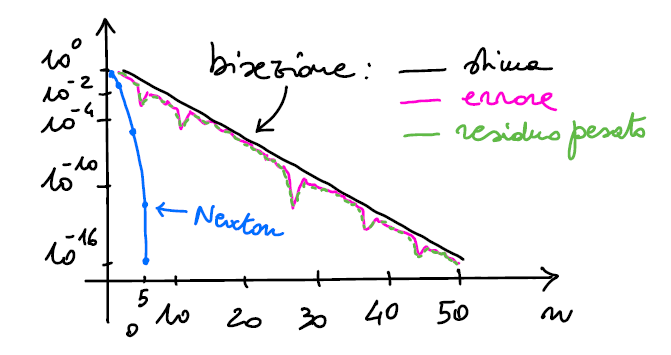
\includegraphics{foto/pagina25}
\end{center}
Perché il metodo di Newton è così veloce? Per capirlo, dobbiamo analizzare l'errore, in particolare quale relazione leghi $e_{n+1}$ con $e_n$ (dove come al solito $e_n=\abs{\,x_n-\xi\,})$\\\\
Enunciamo il risultato sul comportamento dell'errore come teorema, che poi dimostreremo.

\subsection{TEOREMA (sulla velocità di convergenza del metodo di Newton)}
\begin{center}
    \fbox{\begin{minipage}[t]{15cm}%
        Sia $f \in C^2 [a,b]$ e si assuma di essere in ipotesi che garantiscano la convergenza del metodo di Newton e $\xi \in [a,b] : f(\xi) = 0$; sia inoltre $\{x_n\} \subset [c,d] \subseteq [a,b]$ con $f'(x) \neq 0$ $\forall x\in [c,d]$
        allora 
        \[e_{n+1} \le c\ e_n^2, \quad n\ge0, \quad c = \frac{1}{2} \cdot \frac{M_2}{m_1}\]
        \[\text{con } M_2 = \max_{x\in[c,d]}\abs{\,f''(x)\,}, \quad m_1 = \min_{x\in[c,d]}\abs{\,f'(x)\,} > 0\]
    \end{minipage}}
\end{center}
Prima di dimostrare questa disuguaglianza, osserviamo che:
\begin{enumerate}[label=\roman*)]
\item l'ipotesi $\{x_n\} \subset [c,d]$ con $f'(x)\neq0$ in $[c,d]$, come abbiamo già visto nell'analisi del residuo pesato col metodo di bisezione, ci assicura che lo zero $\xi$ è semplice, cioè $f'(\xi) \neq 0$

\item tale ipotesi è soddisfatta ad esempio nelle condizioni del teorema di convergenza dimostrato prima con $[c,d] = [\xi, b]$ nei casi 1) e 3), $[c,d] = [a,\xi]$ nei casi 2) e 4).
\end{enumerate}

\begin{proof}[\unskip\nopunct]
\textbf{Dimostrazione}\\
Applicando la formula di Taylor centrata in $x_n$ e calcolata in $\xi $ , con resto del secondo ordine in forma di Lagrange
\[f(\xi)=f(x_n)+f'(x_n)(\xi-x_n)+\frac{f''(z_n)}{2}(\xi-x_n)^2\]
dove $z_n\in int(x_n,\xi)\subset [c,d]$ e $f(\xi)=0$, da cui 
\[-\frac{f(x_n)}{f'(x_n)}=\xi-x_n+\frac{f''(z_n)}{2f'(x_n)}(\xi-x_n)^2\]
Ma dalla definizione del metodo
\[-\frac{f(x_n)}{f'(x_n)}=x_{n+1}-x_n\]
che inserita nella formula di Taylor porta a 
\[x_{n+1}-x_n=\xi-x_n+\frac{f''(z_n)}{2f'(x_n)}(\xi-x_n)^2\]
ovvero mettendo i moduli
\[e_{n+1}=\abs{\,x_{n+1}-\xi\,}=c_ne_n^2 \quad \text{con} \quad c_n=\frac{1}{2}\frac{\abs{\,f''(z_n)\,}}{\abs{\,f'(x_n)\,}}\]
La successione $\{c_n\}$ è limitata, infatti 
\[\abs{\,f''(z_n)\,}\leq \max_{x \in [c,d]}\abs{\,f''(x)\,}=M_2\]
applicando il teorema di Weierstrass sull'esistenza di massimo e minimo assoluti a $ \abs{\,f''(x)\,}\in C[c,d]$.\\
D'altra parte, applicando lo stesso teorema a  $ \abs{\,f'(x)\,}\in C[c,d]$ abbiamo che 
\[m_1=\min_{x \in [c,d]}\abs{\,f'(x)\,}>0\] 
(perché $\exists \ \overline{x}: m_1=\abs{\,f'(\overline{x})\,} $  e    $f'(\overline{x})\neq 0$   )\\
Otteniamo quindi $\abs{\,f'(x_n)\,}\geq m_1>0$ e infine $c_n \leq \frac{1}{2}\frac{M_2}{m_1}=c$. 
\newline 
\end{proof}

\subsection{Confronto con bisezione}
La relazione di tipo \uline{quadratico}
\[\fbox{$e_{n+1}\leq ce_n^2$}\]
è la chiave per spiegare la velocità di convergenza del metodo di Newton, perché ci dice in sostanza che \uline{l'errore  al passo n+1} è maggiorato da una quantità \uline{proporzionale} (con costante di proporzionalità non dipendente da $n$) al \uline{quadrato} dell'\uline{errore al passo $n$} \\
Si noti la notevole differenza col metodo di bisezione, dove la relazione tra $e_{n+1}$ ed $e_n$ è lineare ($e_{n+1} \approx \frac{1}{2} e_n$, in media).
Per apprezzare l'effetto della relazione quadratica, prima di tutto osserviamo che
\[ ce_{n+1} \leq c \cdot c \cdot e_{n}^2 = ( ce_n)^2\]
Ora, fissiamo $\theta \in (0,1)$:\\
siccome abbiamo assunto che il metodo sia convergente, $ce_n\rightarrow0,\ n\rightarrow\infty$ e quindi $\exists \,\overline{n} : ce_n \leq \theta \quad \forall n \geq \overline{n}$\\
(con $\overline{n}$ dipendente da $\theta$). Applicando la disuguaglianza  $ce_{n+1} \leq (ce_n)^2 \ per \ n \geq \overline{n}$ : 
\[\begin{split}
    ce_{\overline{n}+1} & \le (ce_{\overline{n}})^2 \le \theta^2 \\
    ce_{\overline{n}+2} & \le (ce_{\overline{n}+1})^2\le \left(\theta^2\right)^2 = \theta^4 \\
    ce_{\overline{n}+3} & \le (ce_{\overline{n}+2})^2 \le \left(\theta^4\right)^2 = \theta^8 \\
    \dotso \\
    ce_{\overline{n}+k}& \le (ce_{\overline{n}+k-1})^2 \le \left(\theta^{2^{k-1}}\right)^2 = \theta^{2^k}
\end{split} \]
Adesso, solo per fissare le idee nel confronto col metodo di bisezione, prendiamo $\theta=\frac{1}{2}$. \\
Otteniamo, dopo $k$ iterazioni di Newton a partire da $\overline{n}$ \\
\[e^{\scalebox{.6}{$Newt$}}_{\overline{n}+k}\leq\frac{1}{c}\cdot\left(\frac{1}{2}\right)^{2^k}\]
mentre con $k$ iterazioni del metodo di bisezione 
\[ e^{bisez}_{k}\lesssim \left(\frac{1}{2}\right)^k e_{0}^{bisez}\]
Il confronto sulle $k$ iterazioni va fatto guardando gli esponenti
di $\frac{1}{2}$: nella bisezione l'esponente è $k$ ( cioè cresce linearmente in $k$), con Newton invece l'esponente è $2^k$ (cioè cresce \uline{esponenzialmente} in $k$)\\
Ad esempio per $k=6$ nella stima per la bisezione compare
\[\left(\frac{1}{2}\right)^{6}=\frac{1}{64}\approx 1.6\cdot10^{-2}\]
mentre nella stima per Newton
\[\left(\frac{1}{2}\right)^{2^6}=\left(\frac{1}{2}\right)^{64}\approx 5\cdot10^{-20}\]
Ribadiamo che $\theta=\frac{1}{2}$ è stato scelto arbitrariamente solo per fare un confronto diretto col metodo di bisezione, dove il fattore di riduzione $\frac{1}{2}$ è intrinseco nella costruzione; nel caso del metodo di Newton (per zeri semplici) possiamo dire sostanzialmente che non appena $ce_n<1$ si innesca una riduzione rapidissima dell'errore, di tipo ``quadrati successivi", che viene detta \uline{CONVERGENZA QUADRATICA} (concetto che formalizzeremo nella prossima lezione)
\newpage

\section[Lezione 10 - Ordine di convergenza]{Lezione 10 - Metodo di Newton parte 2, convergenza locale, ordine di convergenza, test di arresto, esempi, altri metodi di linearizzazione}
Partiamo dalla relazione chiave ottenuta nella lezione precedente per l'errore del metodo di Newton:
\[ e_{n+1} = c_n \cdot e_n^2 \leq c e_n^2 \]
\[ c_n = \frac{1}{2} \cdot \frac{\abs{\,f''(z_n)\,}}{\abs{\,f'(x_n)\,}}, \, c = \frac{1}{2} \cdot \frac{M_2}{m_1} \]
con $M_2 = \max\abs{\,f''(x)\,}$ e $m_1 = \min\abs{\,f'(x)\,}>0$ dove $x\in[c,d]$ assumendo che il metodo sia convergente, $f\in C^2[a,b]$ e che $\{ x_n\} \subset{[c,d]} \subseteq{[a,b]}$ con $f'(x)\neq0$ $\forall x\in[c,d]$ \\ 
Da questa abbiamo ottenuto, fissato $\theta\in (0,1)$ e preso $\bar{n}$ tale che 
\[ce_n\leq\theta<1 \quad \forall n\geq\bar{n} \quad \Longrightarrow \quad e_{\bar{n}+k}\leq\frac{1}{c}\,\theta^2, \quad k\geq0\] 
che ci ha fatto capire che per zeri semplici il metodo converge \uline{più che esponenzialmente}.

A questo punto possiamo chiederci: cosa succede se già con la scelta iniziale $x_0$ vale $ce_0<1$? In questo caso avremmo la disuguaglianza \[ ce_n\leq(ce_0)^{2^n} \]
con $n\geq0$. Infatti
\[\begin{split}
    ce_1 & \le (ce_0)^2 \\
    ce_2 & \le (ce_1)^2 \le (ce_0)^4 \\
    \vdots & \\
    ce_n & \le (ce_{n-1})^2 \le (ce_0)^{2^n}
\end{split}\]
Questo ci fa intuire che se $ce_0<1$ cioè 
\[e_0=\abs{\,x_0-\xi\,}<\frac{1}{c}\] 
cioè se prendiamo $x_0$ in un intorno opportuno di $\xi$ zero di $f$ avremo la convergenza con le sole ipotesi che $f \in C^2$ e che $f'(x) \neq 0$ in quell'intorno, perché 
\[ ce_0<1 \quad \Rightarrow \quad (ce_0)^{2^n} \to 0, n\to \infty \quad \Rightarrow \quad e_n \to 0, n \to \infty \]
Si può infatti dimostrare (non lo faremo per brevità) il seguente:

\subsection{TEOREMA (convergenza \uline{locale} del metodo di Newton)}
\begin{center}
    \fbox{\begin{minipage}[t]{15cm}%
        Sia $\xi$ zero di $f$ ed $ \exists\, \delta >0: f\in C^2(I_\delta)$ e $f'(x) \neq 0 \quad\forall x \in I_\delta$, dove $ I_\delta =[\xi-\delta,\xi+\delta]$; inoltre sia $ x_0 \in  I\gamma$  con  $\gamma=\min \left\{ \delta, \frac{1}{c}
        \right\} $ dove 
        \[c=\frac{1}{2}\cdot \frac{\max \abs{\,f''(x)\,}}{\min \abs{\,f'(x)\,}},\quad x\in I_\delta \]
        allora 
        \[ \forall n \geq 0 \quad x_n \in I_\gamma \quad \text{e} \quad e_n \leq \frac{1}{c} (ce_0)^{2^n} \underset{n\to \infty}{\longrightarrow} 0\]
    \end{minipage}}
\end{center}
(nella dimostrazione, per chi volesse provare a farla, un punto chiave è far vedere per induzione che se $x_n \in I_\gamma \Rightarrow x_{n+1}\in I_\gamma$, a cui si arriva mostrando che  $e_{n+1}<e_n<\gamma \ \forall n$ ).
\newline \newline
Come abbiamo già osservato nella lezione precedente, il metodo di Newton pur essendo molto veloce sarebbe poco utile se funzionasse solo in ipotesi forti come ad esempio quelle del teorema di convergenza globale, in cui $e_0$ può può essere grande ma le ipotesi su $f$ sono molto restrittive ($f''$ di segno costante in $[a,b]$).\\
Invece nel teorema di convergenza locale  (che di nuovo, vale la pena di ribadirlo, è un set di condizioni sufficienti (non necessarie) per la convergenza) basta che $ f\in C^2$  e  $ f'\neq 0 $ in un intorno di  $ \xi $ , con la seconda ipotesi che é sempre soddisfatta se lo \uline{zero} è \uline{semplice} perché $f'$ è continua (permanenza del segno di $f'(\xi)$).\\
Conviene a questo punto formalizzare il concetto di ``convergenza quadratica" del metodo di Newton, dando delle definizioni generali sull'ordine di convergenza di un metodo. 

\subsection{DEFINIZIONE \uline{(ordine di convergenza)}}
\begin{center}
    \fbox{\begin{minipage}[t]{17cm}%
Dato un metodo che produce una successione $\{x_n\}_{n\geq 0} $  tale che $\lim_{n \to \infty}x_n=l $  con $l$ limite finito si dice che: 
\begin{enumerate}
\item  il metodo ha ordine di convergenza \uline{almeno} $p>0$ se $ \exists\, c>0$ con ($ c \in (0,1) $ se $p=1$) tale che 
\[e_{n+1}\leq ce_n^p \quad \forall n\]
\item  il metodo ha ordine di convergenza \uline{esattamente} $p>0$ se  $\exists  L>0$ (con $ L\in (0,1)$ se $p=1$ ) tale che:
\[ \lim_{n\to\infty}\frac{e_{n+1}}{e_n^p}=L\]
(dove $L$ è spesso chiamata \uline{costante asintotica} del metodo).\\ 
La convergenza è detta \uline{lineare} se $p=1$, \uline{superlineare} se $p>1$ e in particolare \uline{quadratica} se $p=2$,  \uline{cubica} se $p=3$, $\dotso$
\end{enumerate}
\end{minipage}}
\end{center}
Facciamo alcune osservazioni: nel caso $p=1$ le condizioni $e_{n+1} \leq ce_n, 0<c<1$  (convergenza almeno lineare) e $\lim_{n\to\infty}{\frac{e_{n+1}}{e_n}}=L$ con $L\in(0,1)$ sono condizioni sufficienti per la convergenza. Infatti da $e_{n+1}\leq ce_n$ si ricava 
\[\begin{split}
    e_1 & \leq ce_0, \\
    e_2 & \leq ce_1 \leq c^2e_0, \\
    e_3 & \leq ce_2 \leq c^3e_0, \\
    & \dotso \\
    e_n & \leq c^ne_0
\end{split}\] 
con $c^n\rightarrow 0,n\rightarrow\infty$ perché $c\in[0,1]$ da cui $e_n\rightarrow 0, n\rightarrow\infty$. \\
Analogamente, se $\lim_{n\to \infty}{\frac{e_{n+1}}{e_n}}=L$ con $L\in(0,1)$, preso $\overline{\varepsilon}\in(0,1-L)$ $\exists\, \overline{n}$ tale che 
\[0\leq\frac{e_{n+1}}{e_n}\leq L+\overline{\varepsilon}=c<1 \quad\forall n \geq \overline{n}\] 
cioè $e_{n+1}\leq ce_n$ $\forall n\geq\overline{n}$, da cui ragionando come sopra $e_n \leq c^{n-\overline{n}}e_0 \rightarrow 0$, $n\rightarrow\infty$.\\
D'altra parte, se c'è convergenza, allora necessariamente $L\le 1$.\\
Infatti, se $\lim_{n \to \infty} \frac{e_{n+1}}{e_n} = L > 1$, preso $\overline{\varepsilon} \in (0, L-\overline{\varepsilon})$ $ \exists\, \overline{n}$ tale che $1<L-\overline{\varepsilon} \leq \frac{e_{n+1}}{e_n}$ $\forall n \geq \overline{n}$, quindi $e_{n+1} \geq (L-\overline{\varepsilon})\cdot e_n$ da cui 
\[e_{\overline{n}+1} \geq (L-\overline{\varepsilon}) \cdot e_{\overline{n}}, \dotso, e_n \geq (L-\overline{\varepsilon})^{n-\overline{n}}\quad e_{\overline{n}} \to \infty, n \to \infty\]
e l'errore divergerebbe, cioè non ci sarebbe convergenza.

\subsection{Ordine di convergenza metodo di Newton}
Per quanto riguarda il metodo di Newton, dalla definizione di ordine di convergenza possiamo dire che l'ordine è almeno $p=2$ per zeri semplici perché sappiamo che in tal caso $e_{n+1} \leq ce^2_n$; d'altra parte dall'analisi fatta sappiamo che
\[\frac{e_{n+1}}{e_n^2} = c_n = \frac{1}{2} \cdot \frac{\abs{\,f''(z_n)\,}}{\abs{\,f'(x_n)\,}} \to \frac{1}{2} \cdot \frac{\abs{\,f''(\xi)\,}}{\abs{\,f'(\xi)\,}}\]
per $n \to \infty$ (visto che $z_n \in int(\xi,x_n)$ e $f', f''$ sono continue quindi lo sono $\abs{\,f'\,}, \abs{\,f''\,}$ e si può portare il limite ``dentro le funzioni").\\
Ma allora l'ordine è esattamente $p=2$ se $f''(\xi) \neq 0$, altrimenti $L=0$ e si può dimostrare (non lo faremo) che l'ordine è almeno $p=3$ se $f$ ammette derivata terza in $\xi$.
\newline \newline
Vale la pena di notare che il metodo di bisezione, pur comportandosi ``in media" come un metodo di ordine $p=1$ e costante asintotica $L=1/2$, non ha un ordine definito.\\
Infatti in generale non si può dimostrare che $\exists c: e_{n+1} \leq c\cdot e_n$ con $0<c<1$ e tanto meno che $\lim_{n\to \infty} \frac{e_{n+1}}{e_n} = \frac{1}{2}$.\\
Facciamo infine un'ultima osservazione sull'ordine di convergenza del metodo di Newton: cosa succede quando  $f'(\xi) = 0$ cioè quando lo zero non è semplice?\\
In questo caso l'ordine di convergenza del metodo di Newton scende a $p=1$ con costante asintotica $1-\frac{1}{m}$ dove $m$ è la molteplicità dello zero, cioè la massima derivata che si annulla in $\xi$.\\
Ad esempio, se $m=2$, cioè se $f'(\xi) = 0$ e $f''(\xi) \neq 0$ si ha
\[\frac{e_{n+1}}{e_n} = \frac{e_{n+1}}{e_n^2} \cdot e_n = c_n \cdot e_n = \frac{1}{2} \cdot \frac{\abs{\,f''(z_n)\,}}{\abs{\,f'(x_n)\,}} \cdot e_n\]
Usando la formula di Taylor
\[ f'(x_n)=\underbrace{f'(\xi)}_{=0} + f''(\xi)\cdot (\xi - x_n)+o(e_n) \]
(dove $\alpha_n = o(\beta_n)$ significa che $\lim_{n \to \infty} \frac{\alpha_n}{\beta_n} = 0$), da cui
\[\frac{\abs{\,f'(x_n)\,}}{e_n} \to \abs{\,f''(\xi)\,}, \quad n \to \infty\]
e quindi
\[ \frac{e_{n+1}}{e_n} = e_n \cdot c_n \to \frac{1}{2}, \quad n \to \infty \]

\subsubsection{Perché nel calcolo di $\sqrt2$ con Newton il numero di cifre corrette raddoppia ad ogni iterazione?}
Dopo questo ``excursus" sulla importante nozione di ordine di convergenza, applicata al metodo di Newton, vediamo di spiegare come mai nel caso del calcolo di $\sqrt{2}$ il numero di cifre corrette essenzialmente raddoppia ad ogni iterazione.\\
Quando si parla di cifre corrette, che sono cifre di mantissa, si sta parlando sostanzialmente dell'errore relativo 
\[r_n = \frac{e_n}{\abs{\,\xi\,}}, \quad \xi \neq 0\]
Ora, da $e_{n+1} \leq ce_n^2$ otteniamo 
\[ r_{n+1} = \frac{e_{n+1}}{\abs{\,\xi\,}} \leq c\,\frac{e_n^2}{\abs{\,\xi\,}} = c\,\abs{\,\xi\,}\,r_n^2 \]
Se $c \leq 1$ si ha $r_{n+1} \leq r_n$, cioè l'errore \uline{relativo} al passo $n+1$ è maggiorato dal quadrato dell'errore relativo al passo $n$
\[\begin{split}
    r_1 & \leq r_0^2,\\
    r_2 & \leq r_1^2 \leq r_0^4,\\ 
    & \vdots \\ 
    r_n & \leq r_{n-1}^2 \leq r_0^{2^n}
\end{split}\]
Per fissare le idee, se al passo $k$ $r_k < 10^{-1}$, avremo $r_{k+1} < 10^{-2}$, $r_{k+2} < 10^{-4}$, $r_{k+3} < 10^{-8}$ e con $r_{k+4} < 10^{-16}$ siamo molto sotto la precisione macchina. \\
Questo è proprio quanto succede con $f(x) = x^2 - 2$ in $[1,2]$, dove 
\[ c = \frac{1}{2}\frac{2}{\underset{x \in [1,2]}{\min}2x}  = \frac{1}{2} \cdot \frac{2}{2} = \frac{1}{2} \]
\[c\,\abs{\,\xi\,} = \frac{\sqrt{2}}{2} = \frac{1}{\sqrt{2}} < 1\]
e
\[ r_1 = \frac{1.5 - \sqrt{2}}{\sqrt{2}} \approx 0.06 < 10^{-1} \]
infatti $r_5 < 10^{-16} \Rightarrow x_5 = fl(\sqrt{2})$.

\subsection{Step e residuo pesato}
Prima di fare un paio di esempi ulteriori, è bene discutere alcuni aspetti implementativi.\\
Innanzitutto, osserviamo che richieste computazionali del metodo di Newton sono molto più forti di quelle del metodo di bisezione.\\
Se la bisezione infatti nella versione base ha bisogno solo di conoscere il segno di $f(x)$ (per cui basta come sappiamo errore $< 100\%$ sulla quantità) e col test del residuo pesato (che assume zero semplice e $f \in C^1$) basta saper stimare l'ordine di grandezza del residuo e del peso, ovvero l'ordine di grandezza di $f$ ed $f'$ almeno per $n$ abbastanza grande (infatti per la derivata possiamo accontentarci di una stima tramite rapporti incrementali), col metodo di Newton diventa essenziale poter calcolare con accuratezza sia $f(x_n)$ che $f'(x_n)$ perché gli errori su queste quantità tendono ad essere dominanti nel processo iterativo di calcolo. \\
D'altra parte per il metodo di Newton non abbiamo una stima a priori facile da usare per arrestare le iterazioni.\\
Pensiamo infatti, ad esempio, al caso della convergenza locale e alla stima $e_n \leq \frac{1}{c} \cdot (c\cdot e_0)^{2^n}$.\\
Questa ci dice qualitativamente che c'è convergenza prendendo $x_0$ in un intorno di $\xi$, ma per trovare tale intorno e per usare la stima avremmo bisogno di conoscere $c$, che richiede di saper stimare il minimo di $\abs{f'}$ ma anche il max di $\abs{f''}$ (il che è agevole quando di $f$ sia nota un'espressione analitica semplice ma non in generale).\\
Per fortuna il metodo di Newton può sfruttare una semplice stima a posteriori, il cosiddetto ``STEP" $\abs{x_{n+1} - x_n}$ (la distanza tra le ultime 2 iterazioni).\\
Quando si ha a che fare con un metodo convergente, lo step va a zero per $n \to \infty$ perché $x_n, x_{n+1} \to \xi$; ma una stima dell'errore basata sullo step non è affidabile in generale (anche se stavolta viene usata come stima empirica tipo ``ultima spiaggia").\\
Invece col metodo di Newton lo step è una stima molto buona per costruzione, almeno per $n$ abbastanza grande, perché
\[ STEP(n) = \abs{x_{n+1} - x_n} = \frac{\abs{f(x_n)}}{\abs{f'(x_n)}} \]
visto che 
\[x_{n+1} = x_n - \frac{f(x_n)}{f'(x_n)}\]
cioè per Newton lo \uline{STEP} è per costruzione un \uline{RESIDUO PESATO} ed è già in pratica calcolato ad ogni iterazione visto che basta prendere il modulo di $\frac{f(x_n)}{f'(x_n)}$ che è una quantità chiave nel processo di calcolo.\\
In effetti, la stima a posteriori dello step è generalmente affidabile, soprattutto quando è accompagnata da altri controlli di convergenza.\\
Infatti, sia nel teorema di convergenza globale che in quello di convergenza locale si vede che l'\uline{errore} è \uline{decrescente} ($e_{n+1} < e_n$): quindi per avere garanzia di essere in condizioni di convergenza si può controllare per prima cosa che lo step sia decrescente e poi usarlo come stima accurata dell'errore non appena $\abs{f'(x_n)}$ comincia a stabilizzarsi cioè 
\[\frac{\abs{f'(x_{n-1})}}{\abs{f'(x_n)}} \approx 1\] 
(criterio empirico che abbiamo già discusso nella stima del residuo pesato per il metodo di bisezione).\\
Questo approccio può essere particolarmente utile se si usa un metodo cosiddetto ``ibrido", come sono di solito i metodi adottati dai solutori automatici di equazioni, che in input richiedono $f$, $x_0$ e una tolleranza, accoppiando un metodo ``lento" ma affidabile (ad es. bisezione) per fare alcune iterazioni, partendo poi con un metodo veloce (ad es. Newton o sue varianti) con un controllo di convergenza (tipo decrescita dello step per Newton) e iterando il procedimento finché il metodo veloce non entra in condizioni di convergenza rapida perché parte dell'intorno ``giusto" dello zero (intorno non noto a priori), arrestando le iterazioni con una stima a posteriori (lo step per Newton).\\
Sempre parlando di approccio empirico all'implementazione di un metodo iterativo convergente (non necessariamente un metodo per la soluzione di equazioni) siamo interessati in pratica all'errore relativo, a meno che $\xi = 0$ (o sia piccolissimo).\\
Per avere un test di arresto che funzioni sia per $\xi \neq 0$ (dove conta l'errore relativo) sia per $\xi \approx 0$ (dove conta l'errore assoluto), avendo una stima affidabile dell'errore assoluto si usa spesso un test del tipo
\[stima(n) \leq \varepsilon_a + \abs{x_n} \cdot \varepsilon_r\]
dove $\varepsilon_a$ è una tolleranza assoluta e $\varepsilon_r$ una tolleranza relativa (ad es. $\varepsilon_a = 10^{-10}$, $\varepsilon_r = 10^{-8}$).\\
In questo modo, visto che $\abs{x_n} \to \abs{\xi}$, se $\xi$ è  ben staccato da zero ci si ferma su $\varepsilon_r$, se $\xi = 0$ (oppure $\xi$ è ``piccolissimo") ci si ferma su $\varepsilon_a$.\\
Vediamo come si comporta la stima dello step per il metodo di Newton nel calcolo di $\sqrt{2}$
\begin{center}
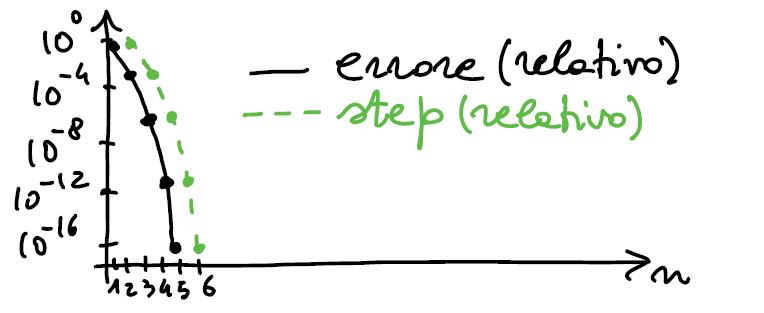
\includegraphics[width=0.5\textwidth]{foto/pag27.JPG}
\end{center}
Si vede che la curva dello step è ``parallela" alla curva dell'errore (quindi è un'ottima stima) ma risulta slittata in avanti di 1: questo è naturale, visto che per avere il residuo pesato $\frac{\abs{f(x_n)}}{\abs{f'(x_n)}}$ al posto di $n$ bisogna essere arrivati al passo $n+1$, 
\[x_{n+1} - x_n = - \frac{f(x_n)}{f'(x_n)}\]
Siccome l'errore decresce velocemente, la stima dello step diventa ancora più affidabile
\[ r_{n+1} = \frac{e_{n+1}}{\abs{\xi}} \ll r_n = \frac{e_n}{\abs{\xi}} \approx \frac{\abs{x_{n+1} - x_n}}{\abs{\xi}}\]
Facciamo ora due esempi di applicabilità del metodo di Newton.

\subsection{Esempio 1 - Metodo di Erone per le radici quadrate}
Abbiamo visto come usare il metodo di Newton per calcolare $\sqrt{2}$ come soluzione dell'equazione algebrica (zero di un polinomio) $f(x) = x^2 - 2 = 0$.\\
L'approccio è generalizzabile al calcolo di $\sqrt{a}$, $a>0$, risolvendo l'equazione $x^2 - a = 0$.\\
Osserviamo che $f(0) = - a < 0$ e $f(b) > 0$ per $b^2 > a$.\\
Visto che $f'(x) = 2x$ e $f''(x) = 2 > 0$ siamo nelle ipotesi del teorema di convergenza globale scegliendo $x_0$: $x^2_0 > a$.\\
Qual è la forma delle iterazioni di Newton in questo caso?
\[\begin{split}
    x_{n+1} & = x_n - \frac{f(x_n)}{f'(x_n)} \\
    & = x_n - \frac{x_n^2-a}{2 x_n} \\
    & = \frac{2 x_n^2 - x_n^2 + a}{2 x_n} \\
    & = \frac{x_n^2 + a}{2 x_n} \\
    & = \frac{x_n}{2} + \frac{a}{2 x_n}, \quad n \ge 0
\end{split}\]
Quindi se $a$ è razionale (in particolare intero) e $x_0$ è razionale il metodo fornisce per costruzione una successione di razionali (frazioni) che converge a $\sqrt{a}$ (quadraticamente perché $\sqrt{a}$ è zero semplice).\\
Questa iterazione era già nota in età ellenistica ed è attribuita al matematico greco Erone di Alessandria (che vi era arrivato non col calcolo differenziale, ignoto all'epoca, ma con metodi geometrici).\\
Lasciamo come ulteriore esercizio la generalizzazione al calcolo di $\sqrt[k]{a} = a^{\frac{1}{k}}$, $k>0$ (ad esempio radice cubica, $k=3$) e anche implementazione e test in Matlab.

\subsection{Esempio 2 - Applicazione del metodo di Newton a un'equazione trascendente}
Il metodo di Newton è applicabile (nelle giuste ipotesi) a qualsiasi equazione del tipo $f(x)=0$ , quindi anche ad equazioni in cui $f$ non è un polinomio o una funzione razionale (rapporto di polinomi), dette equazioni trascendenti (quelle polinomiali/razionali sono dette equazioni algebriche).\\
È il caso di osservare che in realtà anche le equazioni algebriche richiedono metodi numerici: infatti è noto (teoria di Galois) che gli zeri di polinomi di grado $\geq 5$ non sono calcolabili tramite radicali e d'altra parte le stesse equazioni di $2^{\circ}$ grado richiedono il calcolo di $\sqrt{\Delta}$ che va fatto con un metodo approssimato (abbiamo visto sopra come usare Newton che è molto veloce per le radici quadrate). \\
Consideriamo l'equazione trascendente: 
\[f(x)=x-e^{-\alpha x}=0 ,\quad \alpha>0 \]
che si può interpretare come intersezione di grafici (in effetti ha banalmente la forma di punto fisso $x=e^{-\alpha x}$ e la useremo anche nella prossima lezione).\\
Osserviamo che $f \in C^{\infty}(\mathbb{R})$ , $f(0)=-1<0$ , $f(1)=1-e^{-\alpha}>0$ quindi $\exists \  \xi \in (0,1):\ f(\xi)=0$\\
Lo zero è sicuramente unico (in $\mathbb{R}$)\\
\[f'(x)=1+\alpha e^{-\alpha x}>0 \quad \text{($f$ è strettamente crescente)}\]
inoltre \[f''(x)=-\alpha^2 e^{-\alpha x}<0 \quad \text{($f$ è strettamente concava)}\]
\begin{center}
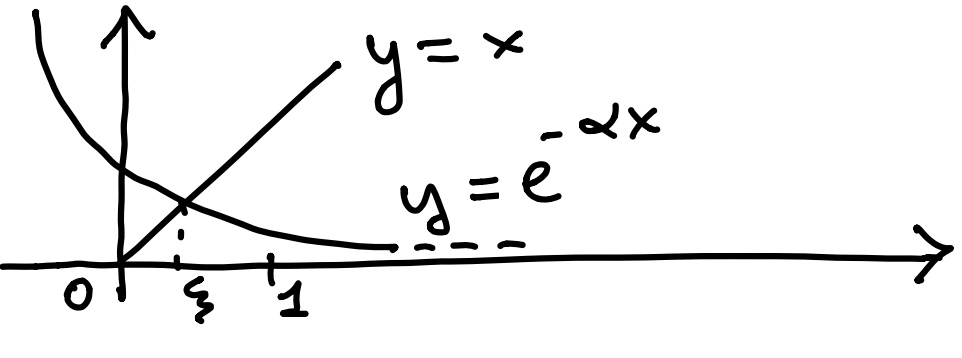
\includegraphics[width=0.5\textwidth]{foto/pag34}
\end{center}
Inoltre 
\[ f'(x) \geq f'(1) = 1+ \alpha e^{-\alpha} \]
e
\[ \abs{f''(x)} = \alpha^2 e^{-\alpha x} \leq \alpha^2, \quad x\in[0,1] \]
vale quindi
\[ c = \frac{1}{2}\,\frac{M_2}{m_1} = \frac{1}{2}\,\frac{\alpha^2}{1+\alpha e^{-\alpha}} \]
per $\alpha \leq 1$ abbiamo che 
\[ c\,\abs{\xi} < \frac{1}{2} \]
da cui otteniamo
\begin{equation*}
    r_{n+1} = \frac{e_{n+1}}{\abs{\xi}} < \frac{1}{2}r_n^2
\end{equation*}
e anche in questo caso ci sarà un raddoppio (almeno) delle cifre corrette ad ogni iterazione (per $\alpha = 1$, $x_5=fl(\xi)=0.5671432904097838$).\\
Lasciamo come esercizio i test in Matlab su questa equazione.

\subsection{Metodo delle corde e delle secanti}
Concludiamo la lezione mostrando in breve altri 2 metodi classici per la soluzione numerica di equazioni non lineari, anch'essi basati su una forma di \uline{LINEARIZZAZIONE} iterativa, il metodo delle CORDE e il metodo delle SECANTI:
\begin{center}
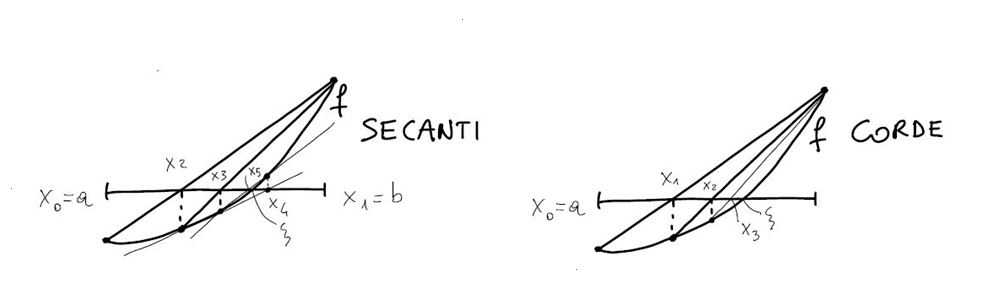
\includegraphics[width=\textwidth]{foto/pag36}
\end{center}
Entrambi i metodi corrispondo a sostituire l'equazione $f(x)=0$ con un'equazione lineare
\[ f(x_n)+q_n(x-x_n)=0 \]
dove nel metodo delle corde $q_n$ è il coefficiente angolare della corda (segmento) per $(x_n,f(x_n))$ e $(b,f(b))$
\[ q_n=\frac{f(b)-f(x_n)}{b-x_n} \]
mentre nel metodo delle secanti $q_n$ è il coefficiente angolare della retta per $(x_{n-1},f(x_{n-1}))$ e $(x_n,f(x_n))$
\[ q_n=\frac{f(x_n)-f(x_{n-1})}{x_n-x_{n-1}} \]
(osserviamo che nel metodo di Newton $q_n=f'(x_n)$).\\
Entrambi i metodi hanno ipotesi di convergenza globale e locale, ad esempio il metodo delle corde converge se $f''$ ha segno costante e $x_0$ è tale che $f(x_0)f''(x_0)>0$; inoltre, il metodo delle corde ha convergenza lineare ($p=1$) mentre il metodo delle secanti ha convergenza superlineare con $p\in(1,2)$. \\
In effetti ci aspettiamo che il metodo delle secanti sia più veloce, perché entrambi rispetto a Newton hanno un rapporto incrementale al posto della derivata
\[ x_{n+1}=x_n-\frac{f(x_n)}{q_n} \]
con $n\geq0$ (corde) e $n\geq1$ (secanti), ma mentre nelle corde un estremo è fisso, nelle secanti per $f\in C^1$
\[ q_n=\frac{f(x_n)-f(x_{n-1})}{x_n-x_{n-1}}\overset{\overset{valor}{medio}}{=} f'(u_n) \]
con $u_n\in int(x_n,x_{n-1})$, quindi se c'è convergenza per il teorema dei 2 carabinieri $u_n\rightarrow\xi$, $n\rightarrow\infty$ e $q_n \rightarrow f'(\xi),\, n\rightarrow\infty$, cioè la secante tende ad essere sempre più ``simile" ad una tangente al crescere di $n$.\\In effetti si può dimostrare (non lo faremo, la dimostrazione richiede nozioni sull'interpolazione lineare che ancora non abbiamo) che l'ordine di convergenza del metodo delle secanti è
\[ p=\frac{1+\sqrt{5}}{2}=1.618\dotso\]
la famosa ``sezione aurea", un numero molto importante in matematica che si incontra in numerose questioni sia teoriche che applicative.\\
Non è difficile far vedere (facoltativo) che per $p>1$ da 
\[ e_{n+1}\leq ce_n^{p} \]
si ricava che $\exists\, c'>0$ tale che
\[ c'e_n\leq(c'e_0)^{p^n} \]
Quindi per $c'e_0<1$ la convergenza è molto rapida (meno di quella di Newton perchè $p<2$ ma comunque più che esponenziale).\\
Il metodo delle secanti risulta quindi una valida alternativa al metodo di Newton quando $f'$ non sia nota o difficile da calcolare (e come Newton è generalizzabile a \uline{sistemi} di equazioni non lineari).
\newpage


\section[Lezione 11 - Iterazioni di punto fisso]{Lezione 11 - Iterazioni di punto fisso, teorema delle contrazioni, convergenza locale, ordine di convergenza, Newton come iterazione di punto fisso}

In questa lezione studieremo equazioni della forma 
\[ x=\phi(x), \ x \in I \subseteq \mathbb{R} \]
dove $\phi \in C(I)$ e $I$ è un intervallo chiuso (non necessariamente limitato) di $\mathbb{R}$ e la loro soluzione numerica tramite semplici iterazioni del tipo
\[ x_{n+1} = \phi(x_n), \ n \geq 0, \ x_0 \in I \]
comunemente dette ``iterazioni di punto fisso".\\
In particolare, vedremo ipotesi che garantiscano la convergenza $x_n \rightarrow \xi$, $n \rightarrow \infty$ dove $\xi = \phi(\xi)$ è detto punto fisso di $\phi$ in $I$ e studieremo l'ordine di convergenza dell'iterazione, scoprendo che il metodo di Newton  può essere interpretato come iterazione di punto fisso. \\
Enunciamo qui sotto un famoso teorema, detto ``teorema delle contrazioni".

\subsection{TEOREMA (esistenza e unicità del punto fisso e convergenza delle iterazioni di punto fisso per una \uline{contrazione})}
\begin{center}
    \fbox{\begin{minipage}[t]{15cm}%
        Sia $\phi:I\subseteq\mathbb{R}\rightarrow\mathbb{R}$ una funzione derivabile nell'intervallo chiuso $I\subseteq\mathbb{R}$, tale che:
        \begin{enumerate}
            \item $\phi(I)\subseteq I$ cioè l'immagine di $I$ tramite $\phi$, $\phi(I)=\left\{y:y=\phi(x), \ x\in I\right\}$, è contenuta in $I$
            
            \item $\exists\,\theta\in(0,1):\abs{\phi'(x)}\leq\theta \ \ \forall x\in I$ 
        \end{enumerate}
        allora 
        \[\exists! \,\xi \in I:\xi = \phi(\xi) \text{ (punto fisso) } \forall x_0 \in I, \ \xi=\lim_{n\to\infty} x_n\]
        \[\text{dove } x_{n+1}=\phi(x_n), \ n\geq0\]
    \end{minipage}}
\end{center}
Prima di dimostrare questo teorema (che può essere esteso ad ambiti molto più astratti (qui ci limitiamo a funzioni reali di variabile reale) come provato dal matematico polacco S. Banach nel 1919 facendolo diventare uno dei risultati chiave dell'analisi matematica contemporanea), facciamo alcune osservazioni:
\begin{enumerate}
    \item l'intervallo $I$ è assunto chiuso, ma può non essere limitato, cioè $I=[a,b]$ con $-\infty < a < b < +\infty$ ma anche $I=[a, +\infty)$ oppure $I = (-\infty,b]$ o addirittura $I=\mathbb{R}$
    \item $\phi$ è una contrazione (di $I$ in sé stesso), cioè contrae le distanze di un fattore $\theta < 1$. Infatti per il teorema del valor medio $\forall x,y \in I$
    \[ \phi(x)-\phi(y)=\phi'(z)(x-y), \quad z \in int(x,y) \]
    da cui
    \[ \abs{\phi(x)-\phi(y)}=\abs{\phi'(z)}\abs{x-y}\leq\theta\abs{x-y}<\abs{x-y}\]
    \item chiaramente la disuguaglianza appena provata implica che $\phi$ è continua in $I$, infatti $\forall x,\overline{x}\in I$
    \[ 0 \leq \abs{\phi(x)-\phi(\overline{x})} \leq \theta \abs{x-\overline{x}} \]
    e quindi per il teorema dei 2 carabinieri
    \[ \abs{\phi(x)-\phi(\overline{x})} \rightarrow 0, \, x \rightarrow \overline{x} \]
    che è equivalente a dire che
    \[ \phi(x) \rightarrow \phi(\bar{x}),\, x \rightarrow \bar{x} \]
\end{enumerate}
\begin{proof}[\unskip\nopunct]
\textbf{Dimostrazione}\\
Cominciamo dimostrando l'$\exists$ di un punto fisso, limitandoci al caso $[a,b]$ limitato: in questo caso basta l'ipotesi $(1)$ e la continuità di $\phi$ (non serve che $\phi$ sia una contrazione). \\
Siccome $\phi$ è continua, tale è 
\[ f(x) = x - \phi(x) \]
Se $a = \phi(a)$ oppure $b = \phi(b)$ allora $a$ oppure $b$ sono punto fisso.\\
Se invece $a \neq \phi(a)$ e $b \neq \phi(b)$ siccome $a \leq \phi(x) \leq b \ \forall x \in [a,b]$ si ha $a - \phi(a) < 0$ e $b - \phi(b) > 0$ cioè $f$ è continua e cambia segno agli estremi 
\[\Longrightarrow \exists\, \xi \in (a,b):f(\xi)=0\] 
cioè \[\exists\, \xi \in (a,b) : \xi = \phi(\xi)\]
La continuità non basta però a garantire l'unicità del punto fisso, come si vede da questo disegno
\begin{center}
    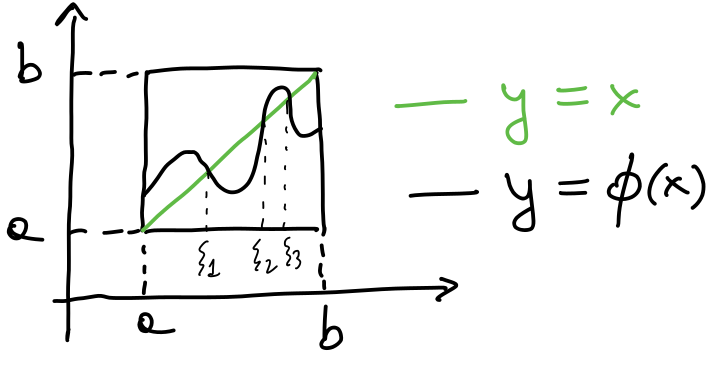
\includegraphics[width=0.5\textwidth]{foto/img1_pag7}
\end{center}
Ma se $\phi$ è una contrazione, l'unicità è assicurata. \\
Infatti se $\exists \xi_1, \xi_2 \in I$ con $\xi_1 \neq \xi_2$ tali che $\xi_1 = \phi(\xi_1)$ e $\xi_2 = \phi(\xi_2)$ allora 
\[\abs{\xi_1 - \xi_2} = \abs{\phi(\xi_1) - \phi(\xi_2)} \leq \theta\abs{\xi_1 - \xi_2}\] 
cioè $\theta \geq 1$ contro l'ipotesi che $\theta < 1$. \\
Resta da dimostrare che $\forall x_0 \in I$, definendo $x_{n+1} = \phi(x_n)$, $n \geq 0$ si ha $\lim_{n\to\infty} \phi(x_n) = \xi$. \\
Ora 
\[e_{n+1} = \abs{x_{n+1} - \xi} = \abs{\phi(x_n) - \phi(\xi)} \leq \theta\abs{x_n - \xi} = \theta e_n\]
da cui 
\[\begin{split}
    e_1 & \leq \theta e_0,\\
    e_2 & \leq \theta e_1 \leq \theta^2 e_0, \\
    & \vdots \\
    e_n & \leq \theta^n e_0 \to 0, \ n\to\infty \text{ perchè } \theta \in (0,1)
\end{split}\]
\end{proof}

\subsection{Stima a priori e a posteriori}
È il caso di fare subito alcune osservazioni importanti: 
\begin{enumerate}
    \item [A)] nel teorema delle contrazioni, la dimostrazione generale è basata sul fatto che la successione $\{ x_n \}$ è di Cauchy e quindi convergente a uno $\xi \in I$ (perché $I$ è chiuso) che è automaticamente punto fisso perché per continuità di $\phi$, 
    \[\xi = \lim x_{n+1} = \lim \phi(x_n) = \phi(\lim x_n) = \phi(\xi)\]
    Ma anche con la dimostrazione scritta sopra, si ottiene la STIMA \uline{A PRIORI} dell'errore \[e_n \leq \theta^n e_0\]
    Se $\theta$ (ed $e_0$) sono noti, questa permette a priori di stabilire il numero di iterazioni sufficiente ad ottenere $\xi$ con una tolleranza $\varepsilon > 0$, risolvendo la disuguaglianza
    \[\theta^n e_0 \leq \varepsilon \Longleftrightarrow e^{n\cdot \log{\theta}} \leq e^{\log{\frac{\varepsilon}{e_0}}} \Longleftrightarrow n \geq \frac{\log{\frac{\varepsilon}{e_0}}}{\log{\theta}} = -\frac{\log{\frac{\varepsilon}{e_0}}}{\abs{\log{\theta}}} = \frac{\log{\frac{e_0}{\varepsilon}}}{\abs{\log{\theta}}}\]
    visto che $\theta \in (0,1)$ e $\log{\theta} < 0$.\\
    Notiamo che la convergenza e la stima ottenuta valgono $\forall x_0 \in I$, cioè le iterazioni di punto fisso che costruiscono (infinite) successioni diverse l'una dall'altra al variare di $x_0$, in ogni caso forniscono successioni che convergono tutte \uline{allo stesso limite} che è l'\uline{unico punto fisso} di $\phi$ in $I$, con una convergenza che è almeno lineare (ordine \uline{almeno} $p=1$) perché $e_{n+1} \leq \theta e_n$
    \item [B)] si può facilmente ottenere una STIMA \uline{A POSTERIORI} dell'errore che spesso è più precisa della stima a priori: basta infatti scrivere
    \[ x_{n+1} - \xi = x_{n+1} - x_n + x_n - \xi \] ma 
    \[x_{n+1}-\xi =\phi(x_n) - \phi(\xi) \underset{\text{VALOR  MEDIO}}{\underset{\uparrow}{=}} \phi'(z_n)(x_n - \xi), \quad z_n \in int(x_n,\xi) \] da cui 
    \[ \phi'(z_n)(x_n - \xi) = x_{n+1}-x_n+x_n-\xi \] ovvero 
    \[ (1-\phi'(z_n))(x_n - \xi) = x_n-x_{n+1} \]
    e passando ai moduli
    \[\frac{\abs{x_{n+1}-x_n}}{\abs{1-\phi'(z_n)}} = e_n \le \frac{\abs{x_{n+1}-x_n}}{1-\theta} \quad \Bigl( 1^\circ \text{ stima a posteriori}\Bigr)\] perchè 
    \[ \abs{\phi'(z_n)} \le \theta < 1 \Longrightarrow \abs{1-\phi'(z_n)} \ge \abs{1-\abs{\phi'(z_n)}} \ge 1 - \theta > 0\] e 
    \[ \frac{1}{\abs{1-\phi'(z_n)}} \le \frac{1}{1-\theta} \]
    In pratica abbiamo fatto vedere che l'errore è stimato dallo STEP $= \abs{x_{n+1}-x_n}$ a meno del fattore $\frac{1}{(1-\theta)}=$ peso.\\
    Se $\theta$ è piccolo, lo step diventa da solo una buona stima dell'errore perchè il peso è $\approx 1$; invece se $\theta$ è vicino ad 1, lo step va corretto per evitare una possibile sottostima.\\
    Ma se $\phi \in C^1(I)$, siccome $z_n \to \xi$ allora $\phi'(z_n) \to \phi'(\xi)$, $n \to \infty$, quindi una stima a posteriori migliore è tendenzialmente la stima empirica (almeno per $n$ abbastanza grande)
    \[e_n = \frac{\abs{x_{n+1}-x_n}}{1-\phi'(z_n)} \approx \frac{\abs{x_{n+1}-x_n}}{1-\phi'(x_n)} \quad \Bigl( 2^\circ \text{ stima a posteriori}\Bigr)\]
\end{enumerate}
Conviene a questo punto fare un esempio

\subsection{Esempio}
Consideriamo l'equazione in forma di punto fisso
\[x = \phi(x) = e^{-\alpha x}, \quad \alpha>0\]
se \uline{$\alpha<1$}, 
\[\abs{\phi'(x)} = \abs{-\alpha e^{-\alpha x}} \le \alpha < 1\]
e quindi $\phi$ contrae le distanze, cioè l'ipotesi (2) del teorema delle contrazioni è soddisfatta con $\theta = \alpha$; d'altra parte, $0<\phi(x) \le 1\, \forall x \in [0,+\infty)$, quindi anche (1) è soddisfatta con $I = [0,+\infty)$.\\
In realtà, siccome $\phi'(x)=-\alpha e^{-\alpha x}<0$, $\phi$ è strettamente decrescente (e positiva), quindi visto che $\phi(0)=1$ e $0<\phi(1)=1-e^{-\alpha}<1$ si ha
\[0 < \phi(x) \le 1 \quad \forall x \in [0,1]\]
cioè $\phi$ è anche una contrazione di $[a,b] = [0,1]$ in se stesso.\\
Allora $\exists$ un unico $\xi$ punto fisso di $\phi$ in $[0,1]$: prendiamo 
\[x_0 = \frac{1}{2} \Longrightarrow e_0 = \abs{x_0 - \xi} \le \frac{1}{2}\]
e la successione $x_{n+1}=\phi(x_n)$, $n \ge 0$ converge a $\xi$ con la stima a priori dell'errore $e_n \le \frac{\alpha^n}{2}$.
\newline \newline
Nel grafico qui sotto mostriamo l'errore effettivo, la stima a priori e la stima a posteriori dello step (non pesato) e dello step pesato da $\frac{1}{(1-\alpha)}$ e da $\frac{1}{(1-\phi'(x_n))}$ con
\[\alpha = 0.2 \Longrightarrow fl(\xi) = 0.8445798674955478\]
\[\alpha = 0.9 \Longrightarrow fl(\xi) = 0.5887032951482605\]
(questi valori sono stati calcolati con il metodo di Newton, si veda Lez.10-Es.2)
\begin{center}
    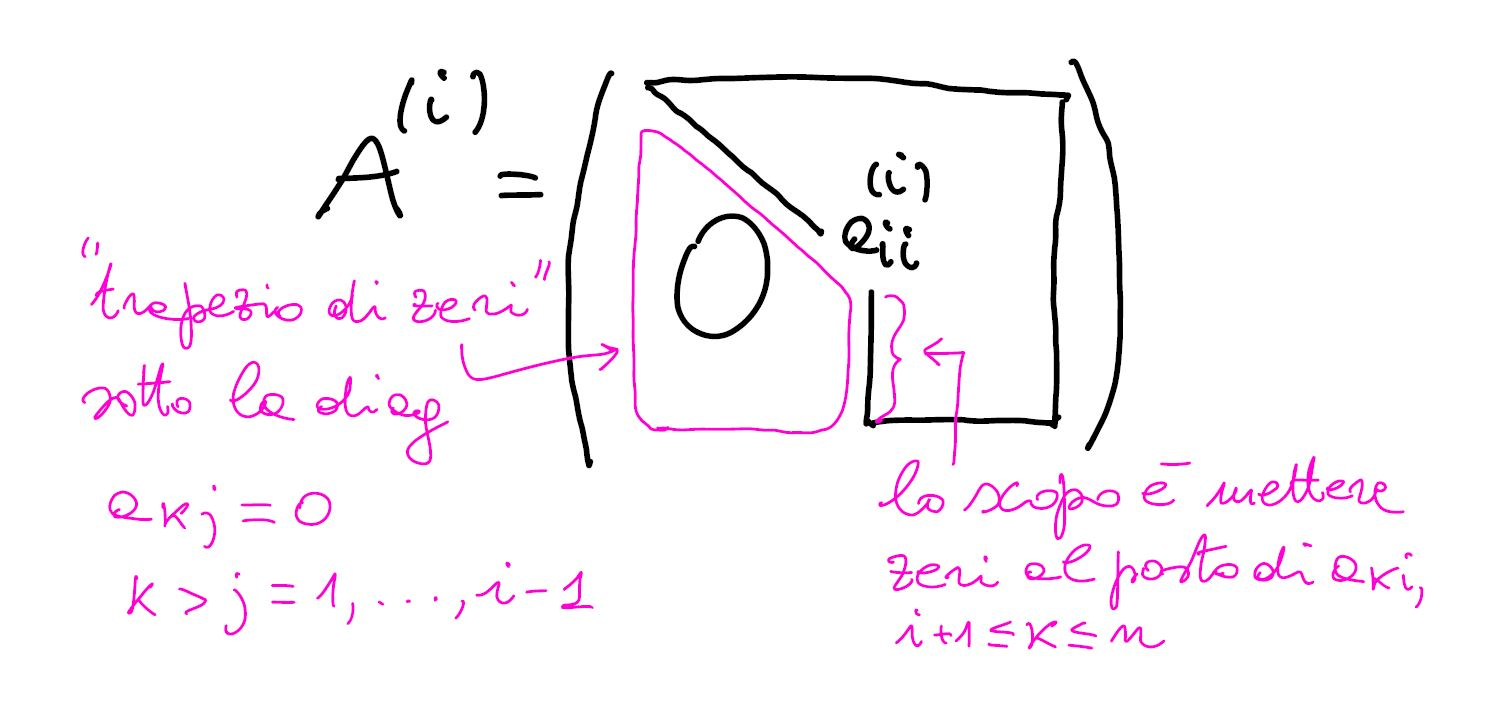
\includegraphics[width=0.8\textwidth]{foto/pag16}
\end{center}
Si vede chiaramente che la convergenza è lineare, che la stima a priori è una sovrastima, molto distante dall'errore per $\alpha = 0.9$: infatti
\[\frac{e_{n+1}}{e_n} = \abs{\phi'(z_n)} \to \abs{\phi'(\xi)}, \quad n \to \infty \quad \text{cioè} \quad \abs{\phi'(\xi)} = \alpha e^{-\alpha \xi} = L\]
è la costante asintotica, il parametro che effettivamente regola la velocità di convergenza ($\alpha$ è solo una stima) perchè per $n$ abbastanza grande
\[e_{n+1} \approx Le_n\]
Qui per $\alpha=0.9$ si ha $L \approx 0.53$ che è ben minore di $\alpha$, mentre per $\alpha=0.2$ si ha $L \approx 0.17$ che è poco minore di $\alpha$.\\
In effetti la $2^\circ$ stima a posteriori,
\[e_n = \frac{\abs{x_{n+1} - x_n}}{(1 - \phi'(x_n))}\]
è una stima aderente dell'errore ma è shiftata in avanti di 1, fenomeno che abbiamo già visto nella stima con lo step nel metodo di Newton, perchè per stimare $e_n$ bisogna essere al passo $n+1$ (step $=\abs{x_{n+1}-x_n}$)
\newline \newline
Dopo aver discusso questo esempio semplice ma significativo, vediamo che anche per le iterazioni di punto fisso vale un risultato di \uline{convergenza locale} (mentre la formulazione generale del teorema delle contrazioni ha
carattere ``globale", visto che $x_0 \in I$ è arbitrario e per la convergenza non è importante che $x_0$ sia vicino a $\xi$).

\subsection{TEOREMA (convergenza LOCALE delle iterazioni di punto fisso)}
\begin{center}
    \fbox{\begin{minipage}[t]{15cm} 
        Sia $\xi$ punto fisso di $\phi \in C^1(I_{\delta}(\xi))$ dove $I_{\delta}(\xi)=[\xi -\delta, \xi +\delta],\, \delta>0$ e sia $\abs{\phi'(\xi)}<1$
        allora
        \[\Rightarrow \exists\, \delta'\le \delta : x_{n+1} = \phi(x_n), \, n\ge 0, \text{ converge a }\xi, \quad \forall\,x_0 \in I_{\delta'}(\xi)\]
    \end{minipage}}
\end{center}
È chiaro il carattere ``locale" di questo risultato, che fornisce
condizioni sufficienti per la convergenza delle iterazioni di punto fisso purchè $x_0$ \uline{sia abbastanza vicino a $\xi$}.
\newline 
\begin{proof}[\unskip\nopunct]
\textbf{Dimostrazione (facoltativa)}\\
Siccome $\phi'$ è continua in $I_{\delta}(\xi)$ tale è $g(x)=\abs{\phi'(x)}-1$, quindi visto che $g(\xi)<0$ per la permanenza del segno $\exists \, \delta'\le \delta$ tale che $g(x)<0$ $\forall x\in I_{\delta}'(\xi)$. Allora $\phi$ è una contrazione in $I_{\delta}'(\xi)$ con 
\[\theta=\max_{x \in I_{\delta}'(\xi)} \abs{\phi'(x)}\]
cioè vale l'ipotesi (2) del teorema delle contrazioni con $I=I_{\delta'}(\xi)$; resta da far vedere che vale (1).\\
Ora, $\forall x \in I_{\delta'}(\xi)$
\[ \abs{\phi(x) - \xi} = \abs{\phi(x) - \phi(\xi)} \leq \theta \abs{x-\xi} \leq \theta \delta' < \delta' \]
cioè $\phi(x) \in I_{\delta'}(\xi)\, \forall x \in I_{\delta'}(\xi)$ e quindi vale anche l'ipotesi (1) del teorema delle contrazioni. \\
Ne consegue che $\forall x_0 \in I_{\delta'}(\xi)$ la successione $x_{n+1} = \phi(x_n), \, n \ge 0$, converge a $\xi$, unico punto fisso di $\phi$ in $I_{\delta'}(\xi)$
\end{proof}

\bigskip
Come per tutti i metodi iterativi, è importante capire quale sia l'\uline{ordine di convergenza} delle iterazioni di punto fisso.\\
Abbiamo già osservato che nel caso di una contrazione l'ordine è almeno $p=1$ perché vale \[e_{n+1}\leq\theta e_n \quad \text{con} \quad \theta \in (0,1)\]
D'altra parte, nell'esempio svolto prima, abbiamo fatto vedere che l'ordine è esattamente $p=1$ se $\phi'(\xi)\neq 0$ con costante asintotica $L=\abs{\phi'(\xi)}$\\
Diamo ora una caratterizzazione completa col seguente:

\subsection{TEOREMA (ordine di convergenza delle iterazioni di punto fisso)}
\begin{center}
    \fbox{\begin{minipage}[t]{16cm}%
        Sia $\xi$ punto fisso di $\phi \in C^p(I),\ p \geq 1$ 
        con $I$ intervallo di $\mathbb{R}$ e supponiamo di essere in ipotesi che garantiscano la convergenza a $\xi$ di $x_{n+1}=\phi(x_n),\ n \geq 0,$ con $x_0 \in I$ (ad esempio le ipotesi del teorema delle contrazioni) \\
        Allora:
        \begin{enumerate}
            \item $\{x_n\}$ ha ordine esattamente $p=1 \ \iff 0<\abs{\phi'(\xi)}<1$
            \item $\{x_n\}$ ha ordine esattamente $p>1 \ \iff \phi^{(j)}(\xi)=0, \ 1\leq j \leq p-1 \ e \ \phi^{(p)}(\xi)\neq 0$
        \end{enumerate}
    \end{minipage}}
\end{center}
\begin{proof}[\unskip\nopunct]
\uline{Dimostrazione}
\begin{enumerate}
    \item si dimostra subito visto che 
        \[e_{n+1}=\abs{\phi'(z_n)}e_n, \ z_n \in int(\xi,x_n)\]
        per il teorema del valor medio, quindi 
        \[\lim_{n\to\infty} \frac{e_{n+1}}{e_n} = \abs{\phi'(\lim z_n)}=\abs{\phi'(\xi)}\]
    \item per 2) utilizziamo la formula di Taylor di grado $p-1$ centrata in $\xi$ con resto $p$-esimo in forma di Lagrange \\
\[x_{n+1}=\phi(x_n)=\underset{\xi}{\underset{\shortparallel}{\phi(\xi)}}+ \phi'(\xi)(x_n-\xi)+\frac{\phi''(\xi)}{2}(x_n-\xi)^2+\dotso+\frac{\phi^{(p-1)}(\xi)}{(p-1)!}(x_n-\xi)^{p-1}+\frac{\phi^{(p)}(u_n)}{p!}(x_n-\xi)^p\]
con $u_n \in int(\xi,x_n)$\\
\begin{itemize}
\item \textbf{Dimostriamo prima $``\Leftarrow"$ (condizione sufficiente)}\\
se $\phi^{(j)}(\xi)=0, \ 1\leq j \leq p-1$ e $\phi^{(p)}(\xi)\neq 0$, da Taylor 
\[x_{n+1}-\xi=\frac{\phi^{(p)}(u_n)}{p!}(x_n-\xi)^p\]
e passando ai moduli
\[\frac{e_{n+1}}{e_n^p}=\frac{\abs{\phi^{(p)}(u_n)}}{p!}\underset{n\to\infty}{\longrightarrow}\frac{\abs{\phi^{(p)}(\xi)}}{p!}\neq 0\]
perché $u_n\rightarrow \xi$, $n\to\infty$ e $\phi^{(p)}$ è continua quindi 
\[\lim \phi^{(p)}(u_n)=\phi^{(p)}(\lim u_n)=\phi^{(p)}(\xi)\]
ovvero $\{x_n\}$ ha ordine esattamente $p$. \\
\item Per \textbf{dimostrare ``$\Rightarrow$" (condizione necessaria)}\\ 
supponiamo per assurdo che $\{ x_n \}$ abbia ordine esattamente $p$ ma che $\exists\ j<p$ tale che $\phi^{(j)}(\xi)\neq 0 $, prendiamo $k=\min\{ j<p:\phi^{(j)}(\xi)\neq0\}$ e scriviamo 
\[\frac{e_{n+1}}{e_n^p} = \frac{e_{n+1}}{e_n^k}\cdot e_n^{k-p}\]
Ora per ipotesi
\[\frac{e_{n+1}}{e_n^p}\rightarrow L \neq 0 \]
d'altra parte con lo stesso ragionamento usato per ``$\Leftarrow$" tramite la formula di Taylor si avrebbe
\[\frac{e_{n+1}}{e_n^k}\to \frac{\abs{\phi^{(k)}(\xi)}}{k!}=L'\neq 0\] 
ma allora
\[\frac{e_{n+1}}{e_n^p} = \frac{e_{n+1}}{e_n^k}\cdot e_n^{k-p}\]
\[\left( \frac{e_{n+1}}{e_n^k} \to L' \text{ ed } e_n^{k-p} \to \infty \text{ perchè } k-p<0 \text{ ed } e_n \to 0 \right) \]
cioè 
\[\frac{e_{n+1}}{e_n^p} \to \infty, \quad n \to \infty\]
contraddicendo l'ipotesi che abbia limite finito.
\end{itemize}
\end{enumerate}
\end{proof}
\bigskip
Ribadiamo che la condizione data è \uline{NECESSARIA} e \uline{SUFFICIENTE}, cioè fornisce una caratterizzazione completa di quando le iterazioni di punto fisso hanno ordine $p>0$.\\
In particolare (e questo ci servirà tra poco) le iterazioni di punto fisso possono avere convergenza \uline{quadratica} ($\phi'(\xi)=0$ e $\phi''(\xi)\ne 0$), \uline{cubica} ($\phi'(\xi)=\phi''(\xi)=0$ e $\phi'''(\xi)\ne0, \dotso$).

\subsection{Metodo di Newton come iterazione di punto fisso}
Per concludere la lezione, mostriamo infatti che il metodo di Newton si può re-interpretare come iterazione di punto fisso e che, in base a quanto visto sopra, si vede subito che ammette convergenza locale e che la convergenza è quadratica per zeri semplici.\\
Infatti l'iterazione di Newton
\[x_{n+1} = x_n - \frac{f(x_n)}{f'(x_n)}, \quad n\ge 0\]
è di tipo punto fisso con
\[\phi(x) = x - \frac{f(x)}{f'(x)}\]
e se $f \in C^k(I)$ con $f'(x)\ne 0 \,\forall x \in I$ intervallo, allora $\phi \in C^{k-1}(I)$.\\
È evidente che $\xi$ è zero (semplice) di $f \iff \xi$ è punto fisso di $\phi$.\\
Inoltre, il teorema di convergenza \uline{locale} per \uline{Newton} (zeri semplici) discende immediatamente dal teorema di convergenza \uline{locale} per le \uline{iterazioni di punto fisso} se $f \in C^2(I_\delta(\xi))$, infatti
\[ \phi'(x) = \frac{d}{dx}\biggl(x-\frac{f}{f'}\biggr) = 1 - \underbrace{\frac{(f')^2 - ff''}{(f')^2}}_{\text{derivata\, del\,rapporto}} = \frac{ff''}{(f')^2}\]
quindi $f(\xi)=0 \Rightarrow \phi'(\xi)=0$ e $\abs{\phi'(\xi)}=0<1$, allora $\exists\, \delta'\le \delta$ tale che l'iterazione di Newton converge come iterazione di punto fisso $\forall x_0 \in I_{\delta'}(\xi)$.\\
D'altra parte, sempre interpretando Newton come iterazione di punto fisso, è immediato che la convergenza per zeri semplici è almeno quadratica perché $\phi'(\xi)=0$ ed è esattamente quadratica se $f''(\xi)\neq0$, utilizzando la caratterizzazione vista sopra (che però richiede $\phi \in C^2$ e quindi $f\in C^3$) infatti:
\[\phi''=\frac{d}{dx}\left(\frac{f f''}{(f')^2}\right)= \underbrace{\frac{\overset{ \downarrow \ derivata \ del \ prodotto}{(f' f''+f f''')(f')^2-2 f' f'' (f f'')}}{(f')^4}}_{\text{ancora\, derivata\, del\, rapporto}}\]
da cui 
\[ \phi''(\xi)=\frac{f''(\xi)}{f'(\xi)}\neq 0 \]
perché 
\begin{equation*}
    f''(\xi)\neq 0 \ ( e \ f'(\xi)\neq0)
\end{equation*}
Non è difficile vedere (come approfondimento facoltativo) che interpretando Newton come iterazione di punto fisso, nel caso di zero multiplo l'ordine di convergenza diventa $p=1$ con costante asintotica 
\[\abs{\phi'(\xi)}=1-\frac{1}{m}\] 
dove $m$ è la molteplicità di $\xi$ (il numero di derivate successive che si annullano in $\xi$) e che se $m$ è nota, l'iterazione
\[x_{n+1}=x_n-m\frac{f(x_n)}{f'(x_n)}=\phi_m(x_n)\]
torna di ordine almeno $p=2$ perché 
\[\phi'_m(\xi)=\lim_{x\to\xi}\phi'_m(x)=0\]
\newpage

% ############ CAPITOLO 3 ######################
\chapter{Interpolazione e approssimazione di dati e funzioni}
\section[Lezione 12 - Interpolazione polinomiale]{Lezione 12 - Ricostruzione di funzioni da dati discreti, interpolazione polinomiale, esistenza e unicità, il problema della convergenza, esempio di Runge}

In questa lezione cominceremo ad occuparci di un argomento molto importante del calcolo numerico dal punto di vista applicativo, ovvero della \uline{ricostruzione (approssimata) di funzioni da dati discreti}, cioè tramite un \uline{campionamento finito}.\\
In particolare, ci concentreremo su 2 tecniche: l'INTERPOLAZIONE (polinomiale e polinomiale ``a tratti") e l'APPROSSIMAZIONE AI MINIMI QUADRATI (di tipo polinomiale).\\
Basti ricordare che le varie tecniche di interpolazione e approssimazione di dati e funzioni sono alla base di molti metodi di enorme interesse applicativo, ad esempio: \uline{grafica} (CAGD), elaborazione di \uline{segnali} e \uline{immagini}, \uline{data science} (machine learning, data mining, $\dotsc$), \uline{discretizzazione} di \uline{modelli differenziali} delle scienze e della tecnologia (\uline{modellistica computazionale:} meccanica, fluidodinamica, meteorologia, elettromagnetismo, \dots).

\subsection{Interpolazione polinomiale}
La prima tecnica che studieremo (limitandoci a funzioni reali di una variabile) è l'interpolazione: dati $n+1$ punti $\left\{ (x_i, y_i) \right\}$ con $y_i=f(x_i)$, $0 \leq i \leq n$, sul grafico di una funzione $f:[a,b] \rightarrow \mathbb{R}$, cerchiamo una funzione $f_n \in \mathcal{F}_n$ (dove $\mathcal{F}_n$ è una opportuna famiglia di funzioni ``semplici"), tale che
\[ f_n(x_i) = y_i, \ 0 \le i \le n \]
cioè tale che il grafico di $f_n$ passi per il grafico di $f$ in corrispondenza delle ascisse di interpolazione $\left\{ x_i \right\}$ (che chiameremo \uline{nodi}, mentre gli $\left\{ y_i \right\}$ sono i valori della funzione campionata)
\begin{center}
    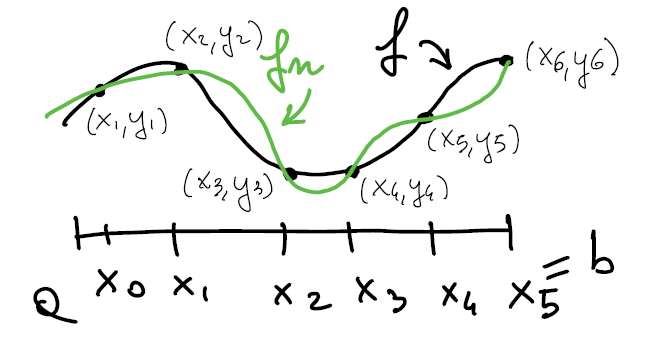
\includegraphics[width=0.5\textwidth]{foto/lez12_img1}
\end{center}
Ribadiamo fin da ora che lo scopo dell'interpolazione è di ricostruire (approssimare) la funzione campionata fuori dal campionamento.\\
Quindi $f_n$ andrebbe scelta in modo che 
\[ dist(f,f_n) \to 0, n \to \infty \]
dove ``dist" è una misura della distanza tra due funzioni, cioè dell'errore che si commette approssimando $f$ con $f_n$. \\
Torneremo più avanti su questo concetto, anticipando che la distanza che useremo è, date $f,g \in C[a,b]$
\[ dist(f,g) = \max_{x \in [a,b]} \abs{f(x) - g(x)} \]
cioè il massimo modulo della differenza tra il valore di $f$ e di $g$ al valore di $x$ in $[a,b]$ (osserviamo che per il teorema di Weierstrass sull'$\exists$ di max e min assoluti di una funzione continua, in questo caso $f-g$, su un intervallo chiuso e limitato, questa distanza è ben definita).\\
Naturalmente avrà senso parlare di convergenza solo dopo che avremo scelto quale sia la famiglia di funzioni $\mathcal{F}_n$ e che sia garantita l'$\exists$ di $f_n \in \mathcal{F}_n$ che interpola la funzione campionata $f$. \\
Una scelta naturale (che è stata anche una delle prime storicamente nel XVIII secolo) è $\mathcal{F}_n = \mathbb{P}_n$, cioè i polinomi di grado $\leq n$ (vedremo che il grado è strettamente legato al problema algebrico dell'$\exists$ e unicità dell'interpolazione).\\
Perché i polinomi? Un primo motivo è che i polinomi sono funzioni facili da gestire e memorizzare (un polinomio è completamente determinato dai suoi coefficienti), infatti $p \in \mathbb{P}_n$ ha la forma 
\[ p(x) = a_0 + a_1x + \dotso + a_n x^n \]
sono facili da calcolare (visto che il calcolo coinvolge solo operazioni aritmetiche, abbiamo tra l'altro lo schema di H{\``o}rner che minimizza il numero di operazioni), sono facili da derivare e integrare, insomma sono dei buoni ``sostituti" di una funzione (purché la stiano approssimando bene). \\
Il primo problema che dobbiamo risolvere è di tipo algebrico: dati $n+1$ punti del grafico di $f$, cioè $n+1$ punti del piano $\{(x_i,y_i)\}_{0\leq i\leq n}$ con $y_i=f(x_i)$, esiste un polinomio $f_n\in\mathbb{P}_n$ che interpola $f$? E se esiste, è unico?\\ Innanzitutto osserviamo che le incognite in questo problema non sono le ``$x$", visto che i nodi di campionamento $\{x_i\}$ fanno parte dei dati del problema, ma sono gli $n+1$ coefficienti $\{a_j\}$. Quindi cercare un polinomio interpolatore in $\mathbb{P}_n$ è una scelta del tutto sensata, perché il numero di incognite è uguale al numero di vincoli (i vincoli di interpolazione $f_n(x_i)=y_i$, $0\leq i\leq n$).\\Scrivendo esplicitamente tali vincoli otterremo un sistema di equazioni con tante equazioni quante sono le incognite. Per capirlo, trattiamo il caso in cui $n=5$ (come nel disegno fatto sopra), cioè cerchiamo un polinomio di grado 5
\[ f_5(x)=a_0+a_1x+a_2x^2+a_3x^3+a_4x^4+a_5x^5 \]
i vincoli di interpolazione sono 
\[ \begin{cases}
    f_5(x_0)=a_0+a_1x_0+\dotso+a_5x_0^5=y_0\\
    f_5(x_1)=a_0+a_1x_1+\dotso+a_5x_1^5=y_1\\
    f_5(x_2)=a_0+a_1x_2+\dotso+a_5x_2^5=y_2\\
    f_5(x_3)=a_0+a_1x_3+\dotso+a_5x_3^5=y_3\\
    f_5(x_4)=a_0+a_1x_4+\dotso+a_5x_4^5=y_4\\
    f_5(x_5)=a_0+a_1x_5+\dotso+a_5x_5^5=y_5\\
\end{cases} \]
che è un sistema \uline{LINEARE} di 6 equazioni nelle 6 incognite $a_0,a_1,\dotso,a_5$.\\ 
\uline{perché} il sistema è \uline{lineare}? Il motivo è che un polinomio di grado $\leq n$ si scrive come \uline{combinazione lineare} degli $n+1$ monomi $1, x, x^2, \dotso, x^n$. In effetti
\[ \mathbb{P}_n = \left\{p(x) = \sum_{j=0}^n a_j x^j \right\} \]
è uno spazio vettoriale di dimensione $n+1$, una cui base sono gli $n+1$ monomi $x^j$, $0 \leq j \leq n$ (che i monomi $\{ x^j \}_{0 \leq j \leq n}$ siano linearmente indipendenti viene dal fatto che se $p \in \mathbb{P}_n$ e $p(x) = 0$ $\forall x \Rightarrow a_j = 0$ $\forall j$) perché un polinomio di grado $\leq n$ non identicamente nullo può avere al massimo $n$ zeri reali (ne ha esattamente $n$, in generale complessi, contati con la loro molteplicità).\\
Formalmente si può scrivere
\[ \mathbb{P}_n = < 1, x, x^2, \dotso, x^n > \]
(dove in generale $< g_1(x), \dotso, g_k(x) >$ indica lo spazio vettoriale generato dalle $k$ funzioni $g_j$, cioè l'insieme di tutte le loro possibili combinazioni lineari) e $\dim(\mathbb{P}_n) = n+1$ (la dimensione è il numero di elementi di una base, cioè di generatori linearmente indipendenti).\\
In generale il sistema lineare di interpolazione è
\[ f_n(x_i) = \sum_{j=0}^n a_j x_i^j = y_i \quad 0 \le i \le n \]
cioè è un sistema lineare di $n+1$ equazioni in $n+1$ incognite e può essere scritto in forma compatta come
\[ V\uline{a} = \uline{y} \]
dove
\[ \uline{a} = 
    \begin{pmatrix}
    a_0 \\ a_1 \\ \vdots \\ a_n
    \end{pmatrix}, \quad
\uline{y} =
    \begin{pmatrix}
    y_0 \\ y_1 \\ \vdots \\ y_n
    \end{pmatrix}
    \in \mathbb{R}^{n+1} \]
sono rispettivamente il vettore dei coefficienti incogniti e il vettore (termine noto) dei valori campionati, mentre $V = (v_{ij}) = (x_i^j)$, con $0 \leq i,j \leq n$ è la matrice del sistema
\[ V =
    \begin{pmatrix}
    1 & x_0 & x_0^2 & \cdots & x_0^n \\
    1 & x_1 & x_1^2 & \cdots & x_1^n \\
    \vdots & \vdots & \vdots & \ & \vdots \\
    1 & x_n & x_n^2 & \cdots & x_n^n
    \end{pmatrix}
    \in \mathbb{R}^{(n+1) \times (n+1)} \]
che viene chiamata ``matrice di Vandermonde" e dipende solo dai nodi di interpolazione (e dal grado $n$).\\
Si può dimostrare che tale matrice è non singolare se e solo se i nodi sono distinti
\[ \det(V) \ne 0 \iff x_i \ne x_j, \quad i \ne j \]
(non dimostreremo direttamente ``$\Leftarrow$", mentre ``$\Rightarrow$" è immediata osservando che se $\exists \ i,j$ tali che $i\neq j$ e $x_i\neq x_j$, allora la matrice avrebbe due righe coincidenti e quindi determinante nullo).\\ 
Quindi vedendo il problema di interpolazione come sistema lineare, se i \uline{nodi} sono \uline{distinti} il sistema ha \uline{soluzione unica}, cioè \uline{$\exists !$} il \uline{polinomio} di grado $\leq n$ \uline{che interpola} gli $n+1$ dati.\\
Dimostreremo questo fatto qui sotto, mostrando con le proprietà dei polinomi che il polinomio interpolatore di grado $\leq n$ su $n+1$ nodi distinti se esiste è necessariamente unico e mostrando che esiste in modo costruttivo, cioè scrivendo tale polinomio in una forma esplicita e specifica (detta forma di Lagrange).

\subsection{Unicità del polinomio interpolatore}
Supponiamo che $\exists$ due polinomi $p,q \in \mathbb{P}_n$ che interpolano, cioè tali che $p(x_i)=y_i=q(x_i)$, $0\leq i \leq n$.\\ Allora il polinomio $p-q \in \mathbb{P}_n$ (ricordiamo che $\mathbb{P}_n$ è uno spazio vettoriale quindi se
\[ p, q \in \mathbb{P}_n \Rightarrow \alpha p + \beta q \in \mathbb{P}_n \quad \forall \alpha, \beta \in \mathbb{R}) \]
e si ha
\[ (p-q)(x_i) = p(x_i) - q(x_i) = 0, \quad 0 \le i \le n \]
cioè $p-q$ avrebbe $n+1$ zeri distinti.\\
Ma per il teorema fondamentale dell'algebra già ricordato sopra, $p-q$ può avere al massimo $n$ zeri distinti, a meno che non sia il polinomio nullo, cioè deve essere
\[ (p-q)(x) = 0 \quad \forall x \Rightarrow p(x) = q(x) \ \forall x \]

\subsection{Esistenza del polinomio interpolatore}
Dati gli $n+1$ nodi distinti $\{ x_i \}_{0 \leq i \leq n}$ consideriamo per ogni nodo fissato (cioè per ogni $i$ fissato) il ``polinomio elementare di Lagrange" così definito
\[ l_i(x) = \frac{N_i(x)}{N_i(x_i)} \]
dove
\[ N_i(x) = (x-x_0)(x-x_1) \dotso (x-x_{i-1})(x-x_{i+1}) \dotso (x-x_n) = \prod_{j=0, \ j\neq i}^n (x-x_j) \]
(nel prodotto viene saltato il termine i-esimo).\\
Osserviamo che $N_i(x) \in \mathbb{P}_n$ è un polinomio di grado effettivo $n$, infatti si ha
\[ N_i(x)=x^n+\dotso \]
mentre $N_i(x_i)$ è un numero $\ne 0$.\\
Quindi $l_i(x) \in \mathbb{P}_n$ e ha grado effettivo $n$,
\[ l_i(x) = \frac{1}{N_i(x_i)}x^n+\dotso \]
Inoltre
\[ l_i(x_k) = \delta_{ik} =
\begin{cases}
0 & i\ne k \\
1 & i=k 
\end{cases} \]
(il cosiddetto ``delta di Kronecker"). Infatti
\[ l_i(x_i) = \frac{N_i(x_i)}{N_i(x_i)} = 1 \]
e per $k\ne i$
\[ N_i(x_k) = (x_k-x_0)\dotso \overbrace{(x_k-x_k)}^{=\,0} \dotso (x_k-x_n) = 0 \]
cioè $N_i (x_k)$,  $k \neq i$ contiene un fattore nullo che annulla il prodotto.\\
Ad esempio 
\[ N_0 (x) = (x-x_1) \dotso (x-x_n) \]
e 
\[ N_0(x_1) = 0 = N_0(x_2) = \dotso = N_0(x_n) \]
allo stesso modo
\[ \begin{split}
    & N_1(x) = (x-x_0)(x-x_2) \dotso (x-x_n) \\
    & N_1(x_0) = 0 = N_1(x_2) = \dotso = N_1(x_n) \\
    & \dotso \\
    & N_n(x) = (x-x_0)(x-x_1) \dotso (x-x_{n-1}) \\
    & N_n(x_0) = 0 = N_n(x_1) = \dotso = N_n(x_{n-1})
\end{split} \]
possiamo allora definire
\[ f_n(x) = \inter_n(x) = \sum_{i=0}^n y_i l_i(x) \]
(polinomio interpolatore di Lagrange).\\
È chiaro che $\inter_n(x) \in \mathbb{P}_n$ (essendo combinazione lineare di polinomi di grado $n$, i polinomi elementari di Lagrange).\\
Verifichiamo che interpola
\[ \begin{split}
    \inter_n (x_k) & = \sum_{i=0}^n y_i l_i (x_k) \\
    & = \sum_{i=0}^n y_i \delta_{ik} \\
    & = y_k \ \delta_{kk} \quad \longleftarrow \quad \text{perché } \delta_{ik}=0, i \ne k\\
    & = y_k, \quad 0 \leq k \leq n
\end{split} \]
Chiameremo $\inter_n(x)$ \uline{il} polinomio interpolatore su $n+1$ nodi distinti (``il" perché è unico) scritto in \uline{forma di Lagrange}.\\\\
Possiamo fare subito la seguente 

\subsection{OSSERVAZIONE 1 (importante)}
Se la funzione che stiamo interpolando è un polinomio in $\mathbb{P}_n$ (cioè di grado $\leq n$), chi è l'interpolatore?\\
L'interpolatore è il polinomio stesso, cioè se $f(x) = p(x) \in \mathbb{P}_n$ allora $\inter_n(x) = p(x)$, perché il polinomio interpolatore è \uline{unico} in $\mathbb{P}_n$ e
$p(x)$ ovviamente interpola se stesso.\\
Questo ci fa capire che un polinomio interpolatore su $n+1$ nodi distinti può avere grado $<n$: ad esempio, se $f(x) = a_1x + a_0$ (cioè $f$ è un polinomio di grado 1), allora $\inter_n(x) = f(x) \ \forall n \ge 1$ e allo stesso modo $f(x) = a_2x^2 + a_1x + a_0$
\[\Longrightarrow \inter_n(x) = f(x) \quad \forall n \ge 2\]
In generale se $f(x) \in \mathbb{P}_k$ allora $\inter_n(x) = f(x) \ \forall n \ge k$
\begin{center}
    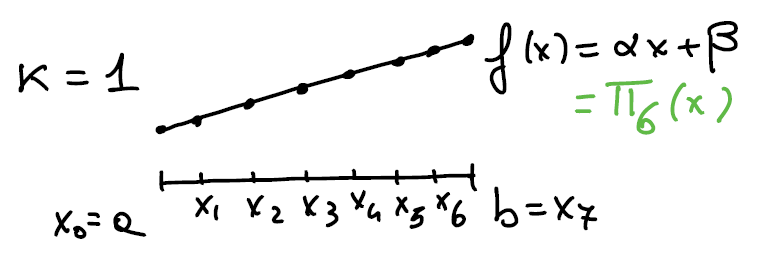
\includegraphics[width=0.6\textwidth]{foto/lez12_img2}
\end{center}
\[\inter_6(x) = f(x) = \alpha x + \beta\]
(per quanti modi di campionamento mettiamo, l'interpolatore resterà \uline{sempre} $\alpha x + \beta$ cioè di grado 1).

\subsection{OSSERVAZIONE 2}
Dal punto di vista teorico, una volta dimostrata l'unicità avremmo automaticamente
anche l'esistenza e viceversa. Infatti, come abbiamo visto il problema di interpolazione in $\mathbb{P}_n$ su $n+1$ nodi distinti è equivalente al sistema lineare di dimensione $n+1 \ \ V\uline{a} = \uline{y}$\\
Ora, se c'è unicità $V\uline{a} = \uline{0} \Rightarrow \uline{a} = \uline{0}$ cioè l'applicazione lineare associata a $V$ è \uline{iniettiva} cioè le colonne di $V$ sono linearmente indipendenti cioè $rango(V)=n+1$ e quindi $V$ è invertibile (ricordiamo che $V \uline{a} = \sum_{k=1}^{n+1} a_k l_k(V)$ dove $l_k(V)$ è la colonna $k$-esima di $V$).\\
D'altra parte, se c'è esistenza $\forall \uline{y} \in \mathbb{R}^{n+1}$ significa che le $n+1$ colonne di $V$ generano tutti i vettori di $\mathbb{R}^{n+1}$ cioè sono una base (l'applicazione lineare è \uline{suriettiva}) e quindi $rango(V)=n+1 \Rightarrow V$ invertibile.\\
Però dal punto di vista applicativo non ci accontentiamo di questo, in particolare è stato importante scrivere il polinomio interpolatore $\inter_n$ in una forma esplicita, la forma di Lagrange (ma ce ne sono altre), utile, come vedremo, anche per studiare altri aspetti come ad es. la \uline{stabilità} dell'interpolazione (nel
senso della ``risposta" dell'interpolazione ad errori sui valori $\{y_i\}$).\\
Possiamo anche osservare che in base all'Osservazione 1, la forma di Lagrange ci dice che i polinomi elementari di Lagrange
\[ \{l_i(x)\}_{0 \le i \le n} \]
sono una base di $\mathbb{P}_n$ (diversa dalla base monomiale $\{x^i\}_{0 \le i \le n}$). \\
Infatti, se $p \in \mathbb{P}_n$ per l'unicità
\[\inter_n(x) = p(x) = \sum_{i=0}^n p(x_i) l_i(x)\]
cioè ogni polinomio di grado $\le n$ si può scrivere come combinazione lineare degli $n+1$ polinomi elementari
(che dipendono \uline{solo} dalla scelta dei nodi di interpolazione $\{x_i\}$)


\subsection{Problema della convergenza}
Dopo aver risolto il problema algebrico dell'interpolazione polinomiale (esistenza e unicità del polinomio interpolatore), ci rimane da discutere l'aspetto chiave della convergenza.\\
Lo scopo dell'interpolazione infatti è di usare l'informazione su una funzione ottenuta tramite un campionamento discreto per ricostruire (in modo approssimato)
la funzione su un intero intervallo.\\
L'uso di polinomi per approssimare funzioni ci è familiare con la formula di \uline{Taylor}; tale formula ha però carattere \uline{locale} (tranne che per la classe di funzioni sviluppabili in serie di Taylor, come $e^x,\ \sin{x},\ \cos{x}, \dotso$).\\
Qui invece siamo interessati a un'approssimazione ``globale" (su tutto $[a,b]$) e la domanda è: è vero che infittendo il campionamento, la successione $\{\inter_n\}$ dei polinomi interpolatori
approssimerà sempre meglio la funzione campionata? Cioè è vero che $\lim_{n \to \infty} \inter_n = f$? \newline \newline
La possibilità di approssimare bene una funzione continua su un intervallo chiuso e limitato $[a,b]$ tramite un opportuno polinomio è assicurata dal ``Teorema di densità di Weierstrass" (che enunciamo solamente, la dimostrazione è molto difficile):


\subsection{TEOREMA (di densità di Weierstrass)}
\begin{center}
    \fbox{\begin{minipage}[t]{15cm}
        $\forall f \in C[a,b]$ fissata e $\forall \varepsilon > 0$
        \[ \exists \ p_{\varepsilon} \in \mathbb{P}: dist(f,p_{\varepsilon}) \le \varepsilon \]
        Dove:
        \begin{itemize}
            \item $\mathbb{P} = \bigcup_{n \ge 0} \mathbb{P}_n$ è l'insieme (che è anche spazio vettoriale) di tutti i polinomi di tutti i gradi
            \item $dist(f,g) = \max_{x\in [a,b]} \abs{f(x)-g(x)}$ è la distanza tra funzioni (continue) che avevamo definito all'inizio
        \end{itemize}
    \end{minipage}}
\end{center}

Cosa significa in pratica che $dist(f,p_{\varepsilon}) \le \varepsilon$? Per capirlo, osserviamo che avendo una distanza tra funzioni (finora avevamo solo una distanza tra numeri $x,y \in \mathbb{R}$ cioè $\abs{x-y}$) siamo in grado di definire cosa sia un intorno
di raggio $\varepsilon >0$ di una $f\in C[a,b]$
\[ I_{\varepsilon}(f) = \{g \in C[a,b] : dist(f,g) \le \varepsilon\} \]
Graficamente, consideriamo un ``tubicino" di ampiezza verticale $2\varepsilon$ costruito intorno al grafico di $f$
\begin{center}
    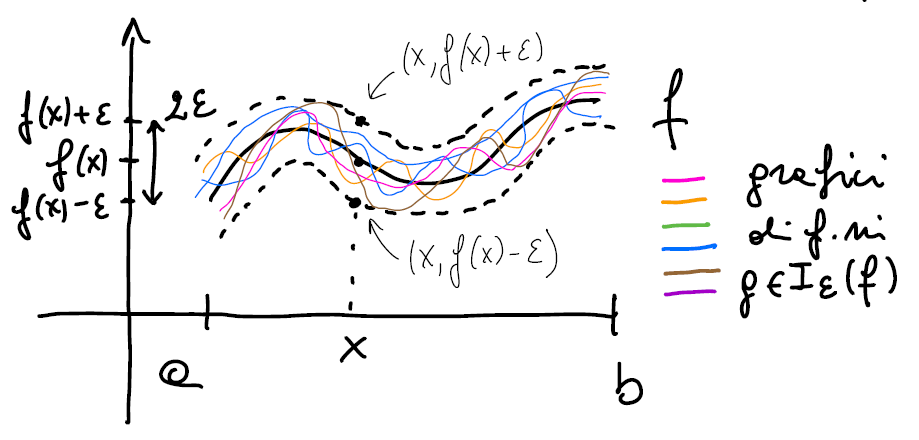
\includegraphics[width=0.8\textwidth]{foto/lez12_img3}
\end{center}
Chi è $I_{\varepsilon}(f)$? \uline{Non} è il ``tubicino" dai contorni tratteggiati ``paralleli" al grafico di $f$ (questo permette solo
la rappresentazione grafica), invece $I_{\varepsilon}(f)$ è l'insieme delle infinite funzioni continue il cui grafico ``vive" nel tubicino, cioè i cui valori $\forall x \in [a,b]$ stanno tra $f(x)-\varepsilon$ e $f(x)+\varepsilon$, cioè 
\[ f(x)-\varepsilon \le g(x) \le f(x)+\varepsilon \]
Ma qualsiasi di queste funzioni $g$ sta approssimando $f$ a meno di $\varepsilon$ su \uline{tutto} l'intervallo $[a,b]$.\\
Quindi, cosa ci sta dicendo il teorema di densità di Weierstrass? Che ogni $f \in C[a,b]$ si può \uline{approssimare} \uline{arbitrariamente} bene
su tutto l'intervallo (perché stiamo parlando del \uline{massimo errore}) con un \uline{opportuno} \uline{polinomio} (di grado opportuno, che dipenderà da $\varepsilon$ e da $f$).\\
Una conseguenza (che non dimostriamo) del teorema di Weierstrass è che $\forall n\ge0\ \exists$ un (unico) polinomio $p_n^* \in \mathbb{P}_n$ tale che
\[ \min_{p \in \mathbb{P}_n} dist(f,p) = dist(f,p_n^*) \underset{n \to \infty}{\longrightarrow} 0 \]
che si chiama ``polinomio di \uline{migliore approssimazione} uniforme" di $f$ in $\mathbb{P}_n$ (purtroppo questo polinomio ottimale
è molto difficile da calcolare); ma visto che è possibile approssimare bene $f \in C[a,b]$ (e d'ora in poi ci muoveremo nell'ambito di funzioni almeno continue) con polinomi, c'è la speranza che infittendo il campionamento, la successione di interpolatori $\{\inter_n\}$ converga nella distanza del max errore a \\$f \in C[a,b]$? Cioè è vero che $\lim_{n \to \infty} \inter_n = f$ nel senso che $dist(f,\inter_n) \to 0,\ n \to \infty$? (la speranza viene dal fatto che infittendo il campionamento stiamo in effetti aumentando l'informazione sulla funzione $f$)\\
Purtroppo la risposta è \uline{\uline{NO}}, cioè in generale \uline{non è vero} che la successione di interpolatori converge alla funzione campionata (come vedremo, la convergenza dipende dalla distribuzione dei nodi $\{x_i\}$).\\
A questo proposito, consideriamo uno dei metodi più usuali di campionamento, cioè un campionamento a \uline{passo costante} in $[a,b]$, cioè
\[ x_i = a+ih, \quad 0\le i \le n, \quad h = \frac{b-a}{n} \]
che consiste nel partizionare $[a,b]$ in $n$ sottointervalli di ampiezza uguale e prendere come nodi di campionamento i loro estremi
\begin{center}
    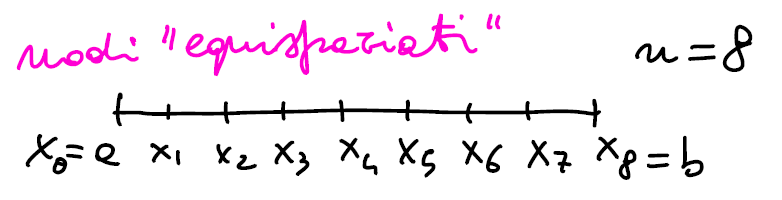
\includegraphics[width=0.6\textwidth]{foto/lez12_img4}
\end{center}
\[ \begin{split}
    x_0 & = a, \\
    x_1 & = a + h, \\
    x_2 & = a + 2h, \\
    & \dotso \\
    x_n & = a+nh = b
\end{split} \]
Questo è un metodo di campionamento del tutto naturale nelle scienze sperimentali e nelle applicazioni tecnologiche, si pensi ad esempio al caso in cui la variabile indipendente è il tempo e si campiona con un passo temporale costante (1 min, 1 sec, 1 millisec, $\dotso$).\\
Bene (anzi, male), purtroppo ci sono funzioni anche molto regolari per cui \uline{l'interpolazione} polinomiale a \uline{passo costante} \uline{non} converge.

\subsection{Funzione di Runge}
Un classico esempio (che non possiamo trattare rigorosamente perché dietro c'è un'intera teoria\\ sull'approssimazione di funzioni) ma che possiamo verificare sperimentalmente ad es. in Matlab, è quello della funzione di Runge
\[ f(x) = \frac{1}{1+x^2}, \ x \in [a,b] = [-5,5] \]
\[ x_i = a+ih = -5+i \cdot \frac{10}{n}, \ 0 \leq i \leq n \]
Si osservi che $f$ è pari ed estremamente
regolare, $f \in C^\infty (\mathbb{R})$ (per inciso, $f$ è la derivata di $\arctan(x)$); ma cosa succede interpolando $f$ a passo costante?
\begin{center}
    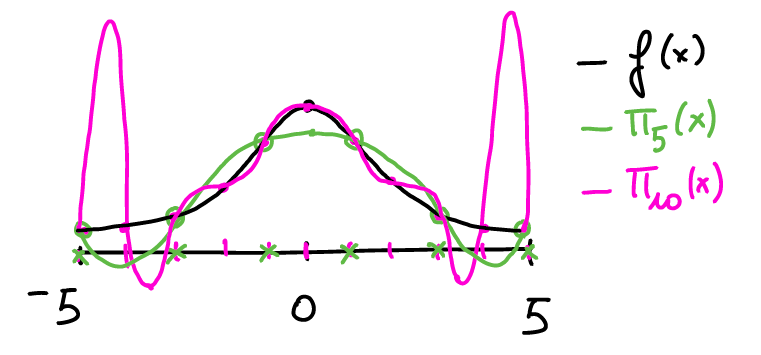
\includegraphics[width=0.5\textwidth]{foto/lez12_img5}
\end{center}
In figura vediamo l'andamento qualitativo dei grafici di $\inter_5(x)$ (6 nodi equispaziati) e di $\inter_{10}(x)$ (11 modi equispaziati): si vede chiaramente che verso gli estremi dell'intervallo, pur infittendo il campionamento, l'approssimazione peggiora.\\
Si può verificare che questo fenomeno persiste al crescere di $n$, in effetti (cosa che si può dimostrare teoricamente e comunque si vede ``sperimentalmente") verso gli estremi si generano oscillazioni sempre più ampie col risultato che addirittura
\[ dist\left(\inter_n^{eq},\ \frac{1}{1+x^2}\right) = \max_{x \in [-5,5]} \abs*{\inter_n^{eq}(x) - \frac{1}{1+x^2}}\underset{n \to \infty}{\longrightarrow} \infty \]
dove $\inter_n^{eq}$ indica l'interpolatore su nodi equispaziati.\\
Questo fenomeno di non convergenza (anzi, di \uline{divergenza}) mostra che la scelta di noti equispaziati non è appropriata per ricostruire una funzione per interpolazione con un unico polinomio di grado $\to \infty$
(la spiegazione teorica dell'esempio di Runge è molto profonda e necessita l'immersione del problema in campo complesso, essenzialmente le singolarità complesse di $f(z)$ che sono $\pm i$ (gli zeri complessi di $1+z^2, \ i^2 = -1$) si trovano ``troppo vicine" all'intervallo in rapporto alla lunghezza dell'intervallo: in effetti ad esempio in $[-3,3]$ ci sarebbe convergenza usando nodi equispaziati (ma come già detto la teoria va ben oltre quello che si può fare in un corso base).\\
Concludiamo la lezione dicendo che ci sono \uline{2 strade} per risolvere il problema della convergenza \\ dell'interpolazione polinomiale, che esploreremo nelle prossime lezioni:
\begin{enumerate}
    \item usare \uline{distribuzioni speciali} dei nodi di campionamento
    \item cambiare tipo di interpolazione, passando dall'interpolazione con un unico polinomio di grado $\to \infty$, all'interpolazione \uline{polinomiale ``a tratti"} in cui si usano polinomi di grado fissato su una suddivisione dell'intervallo in sottointervalli con ampiezza $\to 0$
\end{enumerate}
\newpage
\section[Lezione 13 - Stabilità dell'interpolazione]{Lezione 13 - Formula dell'errore di interpolazione, interpolazione di Chebyshev, costante di Lebesgue e stabilità dell'interpolazione}

Nella lezione precedente abbiamo visto che nell'interpolazione polinomiale c'è un problema sostanziale di possibile \uline{non convergenza}, che dipende dalla distribuzione dei nodi di campionamento e purtroppo si manifesta proprio con una delle distribuzioni più semplici e usuali nella pratica sperimentale: i \uline{nodi equispaziati} (esempio di Runge).\\
Finora però non abbiamo fornito stime dell'errore di interpolazione, e in particolare della distanza
\[dist \left(f,\inter_n \right) = \max_{x \in [a,b]}\, \abs*{\,f(x) - \inter_n(x)\,}\]
dove $f \in C[a,b]$ e $\inter_n$ è il polinomio interpolatore di grado $\le n$ su $n+1$ nodi distinti in $[a,b]$.\\
A questo proposito, enunciamo e dimostriamo qui sotto un classico risultato di rappresentazione.

\subsection{TEOREMA}
\textbf{(rappresentazione di $f(x) - \inter_n(x)$ per $f \in C^{\,n+1}[a,b]$)}
\begin{center}
    \fbox{\begin{minipage}[t]{15cm}
        Siano $f \in C^{\,n+1}[a,b]$ e $\inter_n \in \mathbb{P}_n$ il polinomio interpolatore su $n+1$ nodi distinti $\{x_i\} \subset [a,b]$, 
        allora 
        \[ E_n(x) = f(x) - \inter_n(x) = \frac{f^{(n+1)}(\xi)}{(n+1)!} \omega_{n+1}(x)\]
        dove
        \[\begin{split}
            \omega_{n+1}(x) & = \prod_{i=0}^n (x-x_i) \\
            & = (x-x_0)(x-x_1)\dotso(x-x_n)
        \end{split}\]
        e $\xi \in int(x, x_0, \dotso, x_n)$ (il più piccolo intervallo aperto che contiene tutti i nodi e $x$ fissato in $[a,b]$).
    \end{minipage}}
\end{center}
Prima di dimostrare il teorema, ricordiamo che possiamo sempre pensare di aver ordinato i nodi in modo che $a \leq x_0 < x_1 < \dotso < x_n \leq b$, ma che non è detto che $x_0 = a$ oppure che $x_n = b$ (come accade invece coi nodi equispaziati).\\
Si noti la somiglianza col resto della formula di Taylor (centrata in $\overline{x}$) nella forma di Lagrange
\[ f(x) - \underbrace{t_n(x)}_{\underset{\text{di Taylor}}{\text{polinomio}}} = \frac{f^{(n+1)}(z)}{(n+1)!} (x - \overline{x})^{n+1}, \ \ z \in int(x, \overline{x}) \]
con la differenza che Taylor ha carattere locale mentre l'interpolazione ha carattere globale e al posto di $(x-\overline{x})^{n+1}$ con $x$ in un intorno di $\overline{x}$, compare $\prod_{i=0}^{n} (x-x_i)$ con $x$ che varia in $[a,b]$.\\
\\
\begin{proof}[\unskip\nopunct]
\uline{Dimostrazione} (facoltativa)\\
Fissiamo $x \notin \left\{ x_0, x_1, \dots, x_n \right\}$: infatti se $x=x_i$ è uno dei nodi $f(x_i) - \inter_n (x_i) = 0$ e $\omega_{n+1}(x_i)=0$ perché i nodi sono proprio gli zeri di $\omega_{n+1}(x)$ che è un polinomio di grado $n+1$.\\
Chiamiamo $E_n(x) = f(x) - \inter_n (x)$ (è in effetti l'errore non in modulo ma col segno nel punto $x$), si noti che $E_n \in C^{n+1}[a,b]$, e definiamo la funzione ausiliaria di variabile $z$
\[ g(z) = E_n(z) - \omega_{n+1}(z) \frac{E_n(x)}{\omega_{n+1}(x)}, \quad z \in [a,b] \]
Ora, $g(x) = 0 = g(x_0) = \dotso = g(x_n)$ (visto  che $E_n(x_i) = 0 = \omega_{n+1}(x_i)$). Quindi la funzione $g$ si annulla in $n+2$ punti in $[a,b]$ che sono gli estremi di $n+1$ intervalli
\begin{center}
    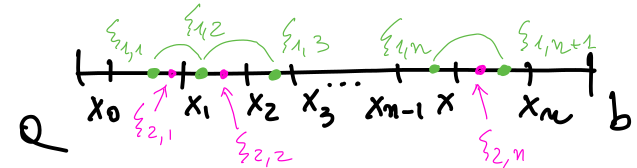
\includegraphics[scale=0.5]{foto/img1_pag6}
\end{center}
(nel disegno abbiamo per esempio $x \in (x_{n-1}, x_n)$).\\
Ricordiamo il \uline{teorema di Rolle} (uno dei risultati cardine del calcolo differenziale in 1 variabile):

\subsubsection{TEOREMA (di Rolle)}
\begin{center}
    \fbox{\begin{minipage}[t]{15cm}%
        Se $\phi \in C[\alpha,\beta]$ è derivabile in $(\alpha,\beta)$ e $\phi(\alpha) = \phi(\beta)$
        \begin{equation*}
            \Rightarrow \exists z \in (\alpha, \beta) : \phi '(z) = 0
        \end{equation*}
    \end{minipage}}
\end{center}
La dimostrazione di basa sul fatto che o $\phi$ è costante in $[\alpha,\beta]$, oppure il max assoluto oppure il min assoluto sono nell'intervallo aperto $(\alpha,\beta)$ e lì la derivata si annulla (la tangente in un punto estremale interno è orizzontale). \\
Allora per il teorema di Rolle applicato a $g$ esistono $n+1$ punti, diciamo $\xi_{1i}, \ 1 \leq i \leq n+1$, ognuno interno ad uno degli intervallini, tali che $g'(\xi_{1i})=0$ (notiamo che $\left\{ \xi_{1,i} \right\} \subset int(x,x_0,\dots,x_n)$). \\
In questo modo sono determinati $n$ intervallini con estremi i punti $\xi_{1,i}$ (si vede il disegno) dove $g'$ si annulla: applicando di nuovo il teorema di Rolle a $g'(x)$ esistono $n$ punti $\xi_{2,i}, \ 1 \leq i \leq n$, ciascuno interno a uno degli $n$ intervallini determinati dai punti $\left\{ \xi_{1,i} \right\}_{1 \leq i \leq n+1}$, tali che $g''(\xi_{2,i}) = 0$ (si noti che $\left\{ \xi_{2,i} \right\} \subset int(\xi_{1,1},\dots, \xi_{1,n+1}) \subset int(x,x_0,\dots,x_n)$). \\
Applicando ripetutamente il teorema di Rolle a $g'',g''',\dotso$, arriviamo infine a dire che $\exists \xi = \xi_{n+1,1} \in int(x,x_0,\dots,x_n)$ tale che $g^{(n+1)}(\xi) = 0$ ma
\[\begin{split}
    g^{(n+1)}(z) & = E_n^{(n+1)}(z) - \omega_{n+1}^{(n+1)}(z) \frac{E_n(x)}{\omega_{n+1}(x)} \\
    & = f^{(n+1)}(z) - (n+1)!\, \frac{E_n(x)}{\omega_{n+1}(x)}
\end{split}\]
perché $\inter_n^{(n+1)}(z) = 0 \,\,\forall\,z$ visto che $\inter_n \in \mathbb{P}_n$ e $\omega_{n+1}^{(n+1)}(z) = (n+1)!$ visto che $\omega_{n+1}(z) = z^{n+1} + \dotso$ (da cui $\omega'_{n+1}(z) = (n+1)z^n + \dotso,\, \omega''_{n+1}(z) = (n+1)nz^{n+1} + \dotso,\,\dotso$).\\
Quindi $\exists \, \xi \in int(x,x_0,\dotso,x_n)$ tale che
\[f^{(n+1)}(\xi) - (n+1)!\frac{E_n(x)}{\omega_{n+1}(x)} = 0\]
che è la rappresentazione cercata.
\end{proof}

\subsection{Stime dell'errore}
Grazie alla rappresentazione esplicita di $E_n(x)$, siamo ora in grado di fare delle stime di
\[\max_{x \in [a,b]} \abs{E_n(x)} = dist\left(f, \inter_n\right)\]
Innanzitutto osserviamo che
\[f \in C^{\,n+1}[a,b] \Longrightarrow f^{(n+1)} \in C[a,b]\]
e quindi per il teorema di Weierstrass sull'esistenza di $max$ e $min$ assoluti di una funzione continua su un intervallo chiuso e limitato
\begin{equation}
    \abs*{f^{(n+1)}(\xi)} \le \max_{x \in [a,b]} \abs*{f^{(n+1)}(x)} = M_{n+1}
\end{equation}
Inoltre comunque $\abs{x-x_i} \le b-a$ quindi
\begin{equation}
    \abs*{\omega_{n+1}(x)} \le (b-a)^{n+1}
\end{equation}
(che è una stima rozza ma valida per qualsiasi distribuzione dei nodi).\\
Quindi in generale possiamo scrivere
\[dist\left(f,\inter_n \right)= \dfrac{f^{n+1}(\xi)}{(n+1)!} \omega_{n+1}(x) 
\overset{(1)}{\leq} M_{n+1} \dfrac{\omega_{n+1}(x)}{(n+1)!} \overset{(2)}{\leq} \overbrace{M_{n+1} \frac{(b-a)^{n+1}}{(n+1)!}}^{stima}\]
Ora, la presenza del fattoriale a denominatore ci potrebbe far sperare che la stima $\to 0,\, n \to \infty$, per $f \in C^{\infty}[a,b]$ (visto che allora la rappresentazione e la stima sono valide $\forall n$): in effetti
\[\frac{(b-a)^{n+1}}{(n+1)!} \to 0, \quad n \to \infty\]
perché è il termine generale della serie di $e^{b-a}$ che converge.\\
Ma sappiamo dall'esempio di Runge che ci sono casi in cui
\[dist\left(f,\inter_n \right) \to \infty, \quad n \to \infty\]
In effetti può succedere che il fattore $M_{n+1}$ nella stima sia non limitato e cresca più rapidamente di 
\[ \frac{(n+1)!}{(b-a)^{n+1}} \]
per $n \to \infty$, cosicché la stima stessa diverge.\\
Infatti è quello che accade (e deve accadere) nell'esempio di Runge (dove l'errore $max$ diverge e quindi la stima diverge).\\
Nel caso dei \uline{nodi equispaziati} si può ricavare una stima più accurata (dimostrazione non richiesta), cioè
\[dist\left(f,\inter_n \right) \le M_{n+1} \frac{h^{n+1}}{4(n+1)}\]
dove $h = \frac{(b-a)}{n}$, ma di nuovo quello che conta è la velocità di crescita di $M_{n+1}$ (che nel caso dell'esempio di Runge cresce più rapidamente addirittura di $(n+1) \cdot h^{-(n+1)}$).\\
La stima ottenuta però ci fa anche capire che ci sono funzioni particolari per cui l'interpolazione sarà sempre convergente, per qualsiasi distribuzione dei nodi (equispaziati, random, sparsi, $\dotso$).\\
Infatti se una funzione $C^{\infty}[a,b]$ ha ad esempio tutte le \uline{derivate equilimitate} (cioè limitate in modulo dalla stessa costante, ovvero $\exists M : M_n \le M \, \forall n$) allora
\[dist\left(f,\inter_n \right) \le M \frac{(b-a)^{n+1}}{(n+1)!} \underset{n \to \infty}{\longrightarrow} 0\]
Esempi sono:
\begin{itemize}
    \item $f(x)=e^x$ per cui $\abs*{f^{(n+1)}(x)} = e^x \le e^b \quad \forall x \in [a,b]$
    \item $f(x)=\sin (x)$ e $f(x)=\cos (x)$ per cui $\abs*{f^{(n+1)}(x)}$ è $\abs*{\sin(x)}$ oppure $\abs*{\cos(x)}$ e quindi $M_{n+1} \le 1$
\end{itemize}
L'esistenza di questi casi $C^{\infty}$ e ``fortunati" non risolve però il problema della convergenza, visto che vorremmo avere un metodo di interpolazione che permetta di approssimare bene funzioni abbastanza generali.

\subsection{Nodi di Chebyshev}
Come abbiamo anticipato, volendo usare un unico polinomio interpolatore $\inter_n$, è necessario cercare distribuzioni speciali dei nodi (visto che i nodi equispaziati, ma anche nodi random o nodi ``scattered" (sparsi) soffrono di situazioni di non convergenza).\\
A questo proposito consideriamo la seguente famiglia di nodi in $[a,b]=[-1,1]$
\begin{center}
    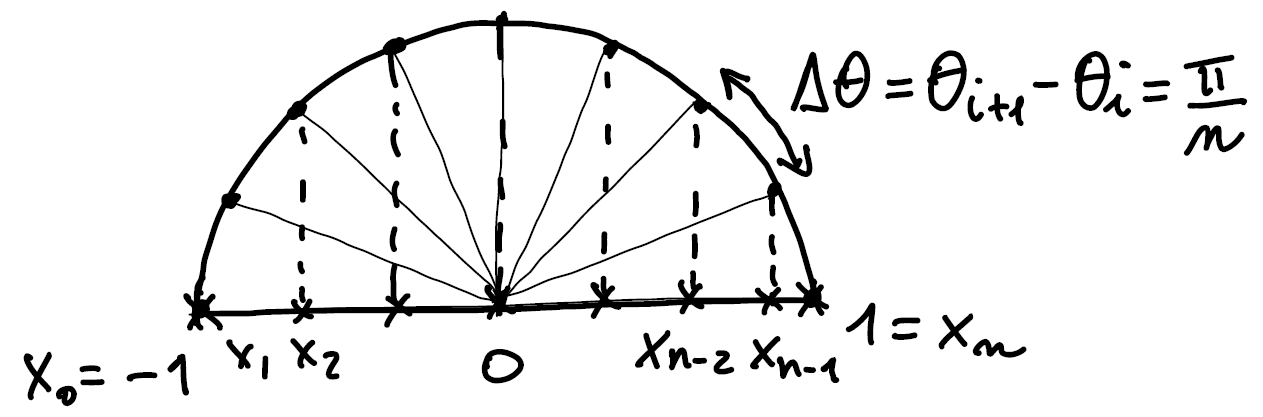
\includegraphics[scale=0.5]{foto/pag-16}
\end{center}
Questi nodi sono ottenuti da punti equispaziati sulla semi-circonferenza di centro (0,0) e raggio 1, cioè corrispondenti agli angoli 
\[\theta_i=i\cdot \frac{\pi}{n}, \quad 0\leq i\leq n,\] 
con 
\[\begin{split}
    \theta_0 & = 0, \\
    \theta_1 & = \frac{\pi}{n}, \\
    \theta_2 & = \frac{2\pi}{n}, \\
    & \dotso \\
    \theta_n & = \frac{n\pi}{n}=\pi,
\end{split}\]
 proiettandoli sull'intervallo $[-1,1]$.\\ 
 Si tratta quindi di coseni 
\[ t_i^{Cheb}=-\cos(\theta_i)=-\cos\left(\frac{i\pi}{n}\right),\quad 0\leq i\leq n \]
(il segno viene cambiato per avere $-1=t_0< t_1<\dotso<t_n=1$) che per costruzione non sono equispaziati ma si addensano  più rapidamente agli estremi dell'intervallo al crescere di $n$ e si chiamano \uline{nodi di Chebyshev} (dal nome del matematico russo che studiò tra i primi il problema dell'interpolazione e approssimazione polinomiale di funzioni continue nel XIX secolo).\\ 
Si può dimostrare (ma la dimostrazione è molto difficile e fa parte di un'intera teoria dell'approssimazione con polinomi) che l'interpolatore su questi nodi, che chiameremo $\inter_n^{Cheb}$, converge uniformemente se $f\in C^k[-1,1]$ per $k>0$, cioè
\[ dist(f,\inter_n^{Cheb})\rightarrow 0 \quad n\rightarrow\infty \]
Per un intervallo generale $[a,b]$ il risultato resta valido se si prendono i nodi ottenuti dalla trasformazione affine
\[ \alpha(t)=\frac{b-a}{2}\cdot t+\frac{b+a}{2},\ \ t\in[-1,1] \]
che manda $[-1,1] \rightarrow [a,b]$, cioè i nodi $x_i^{Cheb}=\alpha(t_i^{Cheb})$ (geometricamente, corrispondono alla stessa costruzione di prima fatta con la semicirconferenza centrata nel punto medio dell'intervallo, $\frac{b+a}{2}$, e di raggio la semilunghezza dell'intervallo, $\frac{b-a}{2}$).\\
In effetti si riesce anche a dare l'ordine di infinitesimo in $n$ per $k$ fissato

\subsection{TEOREMA (convergenza uniforme dell'interpolazione di Chebyshev)}
\begin{center}
    \fbox{\begin{minipage}[t]{15cm}%
        Sia $f \in C^k[a,b], \, k > 0$, 
        allora 
        \[ \exists \, c_k>0 : dist \left(f, \inter_n^{Cheb} \right) \le c_k \frac{\log (n)}{n^k}\]
    \end{minipage}}
\end{center}
Si osservi che 
\[ \frac{\log (n)}{n^k} \to 0, \quad n \to \infty, \quad \forall \, k > 0 \]
più velocemente più grande è $k$; si può far vedere che $c_k$ è proporzionale a 
\[\max_{x \in [a,b]} \abs*{f^{(k)}(x)} \quad \text{(Teorema di Jackson)}\]
È chiaro che se $f$ è almeno $C^1$ (esistono esempi di funzioni solo continue per cui l'interpolazione di Chebyshev non converge) con i nodi di \uline{Chebyshev} abbiamo \uline{risolto} il problema della \uline{convergenza uniforme} dell'interpolazione polinomiale.\\
È il caso di ricordare che esistono altre famiglie di nodi tipo Chebyshev, per cui vale un teorema tipo quello enunciato sopra.\\
Si tratta di nodi non equispaziati che si addensano più rapidamente agli estremi con una legge tipo coseno (non basta prendere nodi non equispaziati e neppure nodi che si addensano agli estremi al crescere di $n$, la chiave è il modo in cui si addensano).\\
Un'altra famiglia, ad esempio, è
\[x_i^{Cheb2} = \alpha(t_i^{Cheb2})\] con
\[t_i^{Cheb2} = - \cos{\left(\frac{\pi}{2}\cdot \frac{2i+1}{n+1}\right)}, \quad 0 \le i \le n\]
(si noti che mentre la prima famiglia comprende gli estremi dell'intervallo, $x_0^{Cheb}=a$ e $x_n^{Cheb}=b$, qui $x_0^{Cheb2}>a$ e $x_n^{Cheb2}<b$, cioè i nodi pur addensandosi agli estremi stanno in $(a,b)$).\\
Dopo aver discusso il problema della convergenza, resta da affrontare un altro problema che sorge in modo naturale, quello della \uline{stabilità} dell'interpolazione polinomiale.\\
Infatti, i valori della funzione campionata in pratica non sono mai noti in modo esatto, ma sono sempre affetti da errori (di arrotondamento, di misura sperimentale, $\dotso$).\\
Supponiamo quindi di avere a disposizione non gli $\{y_i\}$ ma dei valori approssimati $\{\Tilde{y}_i\}$ e di avere una stima dell'errore, del tipo
\[\max_{0 \le i \le n} \abs*{\,\Tilde{y}_i - y_i\,} \le \varepsilon\]
Quindi il polinomio interpolatore sarà $\Tilde{\inter}_n(x)$ invece di $\inter_n(x)$.

\subsection{Convergenza e stabilità del polinomio interpolatore}
La domanda è: come risponde l'interpolatore agli errori sui dati?\\
Quello che dobbiamo fare è una stima di $dist \left(\inter_n, \Tilde{\inter}_n \right)$ per capire come dipenda da $\varepsilon$ (e da $n$).\\
Ci viene in aiuto la forma di Lagrange, per cui l'interpolatore ``esatto" è
\[\inter_n(x) = \sum_{i=0}^n y_i \, l_i(x), \quad y_i = f(x_i)\]
mentre l'interpolatore ``perturbato" (quello costruito coi valori affetti da errore, gli unici che abbiamo veramente a disposizione) è
\[\Tilde{\inter}_n(x) = \sum_{i=0}^n \Tilde{y}_i \, l_i(x)\]
Allora
\[\begin{split}
    \abs*{\,\inter_n(x) - \Tilde{\inter}_n(x)\,} & = \abs*{\,\sum_{i=0}^n y_i \, l_i(x) - \sum_{i=0}^n \Tilde{y}_i \, l_i(x)\,} \\
    & = \abs*{\,\sum_{i=0}^n (y_i - \Tilde{y}_i)\, l_i(x) \,} \\
    & \le \sum_{i=0}^n \overbrace{\abs*{\,y_i - \tilde{y}_i\,}}^{\le\, \varepsilon}\, \abs{\,l_i(x)\,} \\
    & \le \varepsilon \sum_{i=0}^n \abs{\,l_i(x)\,}, \quad \forall\, x \in [a,b]
\end{split}\]
La funzione 
\[\lambda_n(x) = \sum_{i=0}^n \abs*{\,l_i(x)\,}\]
si chiama funzione di Lebesgue: non è un polinomio, ma è la somma di moduli di polinomi (i polinomi elementari di Lagrange) ed è solo continua in $[a,b]$, perché gli zeri di $l_i(x)$ in $(a,b)$, cioè i nodi $\{x_j \in (a,b) : j \ne i\}$, sono punti ``angolosi" (cioè punti di non derivabilità di $\abs{\,l_i(x)\,}$, per cui $\abs{l_i}\in C[a,b]$ ma $\abs{l_i} \notin C^1[a,b]$
\begin{center}
    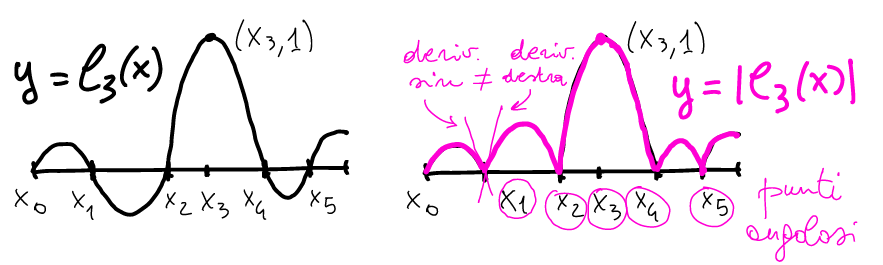
\includegraphics[scale=0.8]{foto/lez13_img2}
\end{center}
Prendendo il max in $[a,b]$ da ambo i lati della disuguaglianza 
\[ \abs*{\inter_n(x)-\tilde{\inter}_n(x)}\leq \varepsilon  \sum_{i=0}^n \abs{l_i(x)}=\varepsilon\lambda_n(x) \]
Si ottiene
\[ dist\left(\inter_n,\tilde{\inter}_n\right)\leq \Lambda_n \]
dove 
\[\Lambda_n= \max_{x\in[a,b]}\lambda_n(x)\]
viene detta \uline{COSTANTE DI LEBESGUE} dei nodi di interpolazione.\\
Si noti infatti che tale quantità (costante in $x$) dipende \uline{solo} dai nodi $\{ x_i \}$ e agisce come un \uline{coefficiente}\\ \uline{di amplificazione} del massimo errore $\varepsilon$ sui dati.\\
Si può dimostrare (ma è difficile) che esistono delle costanti $\alpha_1, \alpha_2, \alpha_3 > 0$ tali che
\begin{enumerate}
    \item $\Lambda_n \geq \alpha_1 log(n)$ per \uline{qualsiasi} distribuzione di nodi
    \item $\Lambda^{eq}_n \sim \alpha_2 \frac{2^n}{nlog(n)}, \ n \to \infty, \ \alpha_2 = \frac{2}{e} \simeq 0.74$
    \item $\Lambda^{Cheb}_n \leq \alpha_3 log(n), \ \alpha_3 \simeq \frac{2}{\pi} \simeq 0.64$
\end{enumerate}
cioè, la costante di Lebesgue cresce almeno come $\log(n)$, ma nel caso dei nodi \uline{equispaziati} ha crescita sostanzialmente \uline{esponenziale}, mentre nel caso delle varie distribuzioni dei nodi di tipo \uline{Chebyshev} ha crescita \uline{logaritmica} e quindi quasi ottimale.\\
La stima ottenuta mostra che l'interpolazione su \uline{nodi equispaziati}, oltre ad essere in generale non convergente, è anche \uline{instabile}, mentre l'interpolazione di \uline{Chebyshev} oltre ad essere convergente (per $f \in C^k, k>0$) è anche sostanzialmente \uline{stabile}, perché $\log(n)$ cresce molto lentamente.\\
Ad esempio per $n=30$ si ha:
\begin{itemize}
\item $\Lambda^{eq}_{30} \simeq 8 \cdot 10^6$
\item $\Lambda^{Cheb}_{30} \lesssim 2.2$
\end{itemize}
e per $n=50$:
\begin{itemize}
\item $\Lambda^{eq}_{50} \simeq 4 \cdot 10^{12}$
\item $\Lambda^{Cheb}_{50} \lesssim 2.49$
\end{itemize}
Questo significa che anche per le classi di funzioni su cui convergerebbe (ad esempio funzioni con derivate ``equilimitate", come visto prima), in pratica l'interpolazione polinomiale su nodi equispaziati è inutilizzabile appena $n$ cresce.\\
Invece l'interpolazione di Chebyshev è un'ottima scelta, visto che partendo dalla disuguaglianza
\[ \abs*{f(x) - \tilde{\inter}_n (x)} \leq \abs*{f(x) - \inter_n (x)} + \abs*{\inter_n (x) - \tilde{\inter (x)}} \]
e prendendo il max in $[a,b]$ da ambo i lati, otteniamo
\[ dist\left(f, \tilde{\inter}_n\right) \leq \underbrace{dist \left(f, \inter_n \right)}_{\text{convergenza}} + \underbrace{dist \left( \inter_n, \tilde{\inter}_n\right)}_{\text{stabilità}} \underbrace{\lesssim}_{\text{per i nodi di Cheb}} c_k \frac{\log(n)}{n^k} + 0.64\cdot \log(n) \cdot \varepsilon \]
se $f \in C^k [a,b], k>0$ e $\max\abs{y_i - \tilde{y_i}} \leq \varepsilon$\\
C'è però uno svantaggio evidente nell'interpolazione di Chebyshev: è necessario interpolare su \uline{quei} particolari nodi per garantire convergenza e stabilità, mentre potrebbe essere più semplice o più naturale campionare su altri nodi (equispaziati, sparsi, $\dotso$).\\
In questi casi cosa si può fare? Vedremo nella prossima lezione che il problema della convergenza (e della stabilità) è risolubile infittendo il campionamento con distribuzioni arbitrarie dei nodi, tramite le tecniche di interpolazione \uline{polinomiale a tratti}.
\newpage

\section[Lezione 14 - Interpolazione polinomiale a tratti]{Lezione 14 - Interpolazione polinomiale a tratti, convergenza e stabilità, interpolazione spline}
In questa lezione studieremo dei metodi di interpolazione che permettono di risolvere il problema della convergenza dell'interpolazione polinomiale, in particolare nel caso di un campionamento a passo costante (nodi equispaziati).

\subsection{Interpolazione polinomiale a tratti}
L'idea è, invece di prendere un unico polinomio interpolatore
con grado $\rightarrow\infty$, di costruire funzioni interpolanti polinomiali ``\uline{a tratti}", ottenute ``incollando" per continuità interpolatori di \uline{grado fissato} su una partizione dell'intervallo $[a,b]$ in intervallini consecutivi.\\ 
Assumiamo che 
\[ a=x_0<x_1<x_2<\dotso<x_n=b \]
Il parametro che ci permette di infittire il campionamento sarà $h=\max\Delta x_i$, dove $\Delta x_i= x_{i+1}-x_i$, $0\leq i\leq n-1$\\
Osserviamo che $h\rightarrow0\Rightarrow n\rightarrow\infty$ mentre il viceversa non vale in generale (è vero ad esempio però coi nodi equispaziati per cui $h=\frac{b-a}{n}$).\\ 
Infatti aumentando solamente il numero di nodi potremmo infittirli in una parte dell'intervallo, senza aumentare l'informazione sulla funzione campionata nella parte restante
\begin{center}
    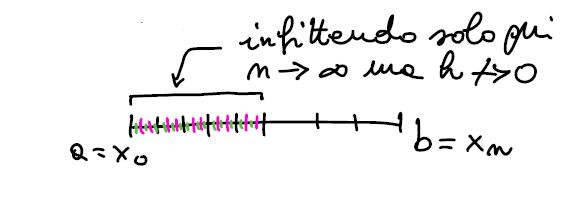
\includegraphics[scale=0.5]{foto/calcolo}
\end{center}
Per capire la tecnica, iniziamo con un disegno dell'interpolazione
\begin{center}
    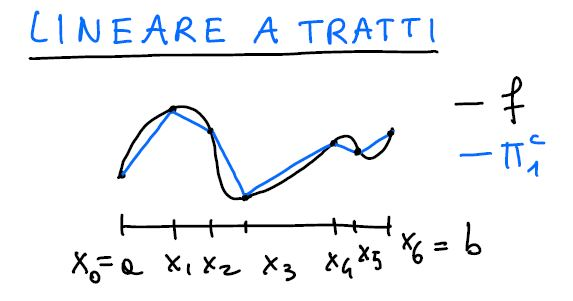
\includegraphics[scale=0.5]{foto/calcolo2}
\end{center}
e qui sotto dell'interpolazione\\
\begin{center}
    \includegraphics[scale=0.5]{foto/calcolo3}
\end{center}
Nel primo caso l'interpolante si ottiene tracciando i tratti di retta congiungenti i 2 punti del grafico corrispondenti a 2 nodi consecutivi.\\
Nel secondo caso l'interpolante si ottiene tracciando le ``paraboline" corrispondenti a ``pacchetti" di 3 nodi consecutivi (con un nodo di raccordo tra 2 pacchetti consecutivi) ovvero
\[\begin{split}
    x_0,x_1,x_2 & \rightarrow 1^\circ \text{ pacchetto}\\
    x_2,x_3,x_4 & \rightarrow 2^\circ \text{ pacchetto}\\
    x_4,x_5,x_6 & \rightarrow 3^\circ \text{ pacchetto}
\end{split}\]
Osserviamo subito che questo è possibile perché $n=6$ è pari.\\
In generale, per costruire una funzione interpolante di grado $s$ a tratti, abbiamo bisogno di pacchetti consecutivi di $s+1$ nodi distinti (che individuano un unico polinomio interpolatore ``locale" di grado $s$), con un nodo di raccordo tra 2 pacchetti consecutivi.\\
Perché questo sia possibile bisogna che $n$ sia multiplo intero di $s$, cioè $n = k \cdot s$\\\\
\begin{minipage}{0.33\textwidth}
\begin{center}
    pacchetti\\
    $x_0, x_1, \dotso, x_s$\\
    $x_s, x_{s+1}, \dotso, x_{2s}$\\
    $x_{2s}, x_{2s+1}, \dotso, x_{3s}$\\
    $\dotso$\\
    $x_{(k+1) \cdot s}, \dotso, x_{ks}$
\end{center}
\end{minipage}
\begin{minipage}{0.33\textwidth}
\begin{center}
    tratti\\
    $[x_0, x_s]$\\
    $[x_s, x_{2s}]$\\
    $[x_{2s}, x_{3s}]$\\
    $\dotso$\\
    $[x_{(k-1) \cdot s}, x_{ks}]$
\end{center}
\end{minipage}
\begin{minipage}{0.33\textwidth}
\begin{center}
    interpolatori locali\\
    $\inter_{s,1}$\\
    $\inter_{s,2}$\\
    $\inter_{s,3}$\\
    $\dotso$\\
    $\inter_{s,k}$
\end{center}
\end{minipage}

\bigskip
La funzione interpolante, che chiameremo $\inter_s^c$ (interpolante ``composta" di grado $s$ a tratti) \uline{non} è (in generale) un polinomio ed è ottenuta ``incollando" per continuità nei nodi di raccordo i vari polinomi interpolatori locali di grado $s$, $\{ \inter_{s, i}\}$, $1 \leq i \leq k$.\\
Tale funzione polinomiale di grado $s$ a tratti è \uline{UNICA}, perché sono unici gli interpolatori locali $\inter_{s,i}$ e interpola perché $\forall x_j$ avremo che $x_j \in [x_{(i-1) s}, x_{i s}]$ per un certo $i$ e quindi
\[ \forall j \quad \inter_s^c (x_j) = \inter_{s,i} (x_j) = y_j = f(x_j) \]
Osserviamo fra l'altro che per l'unicità se $f \in \mathbb{P}_m, \ m \leq s \ \Rightarrow \inter_s^c = f$ (cioè se $f$ è un polinomio di grado $\leq s$, allora l'interpolante a tratti di grado $s$ è quello stesso polinomio).\\
Rispetto all'interpolazione con un unico polinomio $\inter_n$ il cui grado $n$ viene mandato ad $\infty$, l'aspetto chiave nella costruzione di $\inter_s^c$ è che $s$ è \uline{fissato} (e per infittire il campionamento si prende\\
$h=\max \ \Delta x_i \to 0$, in modo da infittire in tutto l'intervallo $[a,b]$).\\
Il caso dei nodi equispaziati rientra nella costruzione con
\[ x_i = a+ih, \ 0 \leq i \leq n, \ h = \frac{b-a}{n} \]
e corrisponde ad infittire a passo costante il campionamento (ma la costruzione è possibile per qualsiasi distribuzione di $n+1$ nodi purché $n$ sia multiplo di $s$).\\
Il vantaggio dell'interpolazione polinomiale a tratti è che garantisce la \uline{convergenza uniforme}, cioè 
\[ dist(f, \inter_{s}^{c}) \to 0, \ h \to 0 \]
Enunciamo ora, e dimostriamo per $s=1$, un risultato generale sulla convergenza (e sull'ordine
di infinitesimo dell'errore in $h$)

\subsection{TEOREMA (convergenza uniforme dell'interpolazione polinomiale a tratti)}
\begin{center}
    \fbox{\begin{minipage}[t]{15cm}%
        Siano $f \in C^{s+1}[a,b], \ s \geq 0$ e $\{x_i \} \subset [a,b] \ n+1$ nodi distinti, con $n$ multiplo di $s$.\\
        Allora
        \[ \exists k_s > 0: dist(f, \inter_s^c) \leq k_s  h^{s+1}, \ h = \max \ \Delta x_i \]
    \end{minipage}}
\end{center}

\begin{proof}[\unskip\nopunct]
\textbf{\uline{Dimostrazione}}\\
Dimostriamo il teorema per $s=1$ (interpolazione lineare a tratti)\\
Osserviamo che
\[ \begin{split}
    dist(f, \inter_{1}^{c}) & = \max_{x \in [a,b]} \abs*{f(x) - \inter_{1}^{c} (x)} \\
    & = \max_{0 \le i \le n-1}\, \max_{x \in [x_i, x_{i+1}]} \abs*{f(x) - \inter_{1}^{c} (x)}
\end{split} \]
(perché il max su tutto $[a,b]$ è il massimo dei max sui singoli intervallini)
\[= \max_{1 \le i \le n}\, \max_{x \in [x_{i-1},x_i]} \abs{f(x) - \inter_{1,i}(x)}\]
(perché in $[x_{i-1}, x_i] \,\inter_1^c$ è il polinomio interpolatore locale di grado 1 $\inter_{1,i}$ su $(x_{i-1}, y_{i-1})$ e $(x_i, y_i)$).\\
Ora ricordando la stima dell'errore di interpolazione polinomiale a grado $s$ ricavata dalla scorsa lezione
\[\max_{x\in [\alpha , \beta]}\abs*{f(x) - \inter_{s}(x)} \le \max_{x\in [\alpha , \beta]} \abs{f^{(s+1)}(x)} \cdot \frac{h^{s+1}}{4(s+1)} \]
valida per $f \in C^{s+1}[\alpha, \beta]$ e $h = \frac{b-a}{s}$, e applicandola per $s=1$ e $[\alpha,\beta] = [x_{i-1},x_i]$, otteniamo
\[ \max_{x\in [x_{i-1},x_i]}\abs{f(x) - \inter_{1,i}(x)} \le \max_{x\in [x_{i-1},x_i]}\abs{f''(x)} \cdot \frac{h^2}{8} = M_{2,i} \frac{h^2}{8} \]
da cui
\[ \begin{split}
    dist(f, \inter_{1}^{c}) & = \max_{1 \le i \le n}\, \max_{x \in [x_{i-1},x_i]} \abs*{f(x) - \inter_{1,i}(x)} \\
    & \le \frac{h^2}{8} \max_{1 \le i \le n} M_{2,i} \\
    & = \frac{M_2}{8}h^2
\end{split} \]
con $M_2 = \max_{x\in[a,b]} \abs{f''(x)}$ (di nuovo perché il $\max$ di $\abs{f''(x)}$ su $[a,b]$ è il massimo dei $\max$ di $\abs{f''(x)}$ sui singoli intervallini).\\
\end{proof}
\bigskip
Vale la pena di notare che l'interpolazione lineare a tratti converge anche se $f \in C^1[a,b]$ con $dist(f,\inter_1^c)\leq ch, \, c>0$, e perfino per $f$ solo continua in $[a,b]$, anche se in questo caso si sa solo che $dist(f,\inter_1^c) \rightarrow 0$, $h \rightarrow 0$ (non facciamo le dimostrazioni).\\
La dimostrazione fatta per $s=1$ si può adattare facilmente: $s>1$ nel caso di nodi equispaziati, ottenendo $K_s=\dfrac{M_{s+1}}{4(s+1)}$ (dimostrazione facoltativa).

\subsection{Stabilità interpolazione polinomiale a tratti}
Possiamo dire qualcosa anche sulla stabilità dell'interpolazione polinomiale a tratti, sempre nel caso di nodi equispaziati che sappiamo essere fortemente instabile per l'Interpolazione polinomiale standard.\\
Infatti, detta $\widetilde{\inter_1^c}$ l'interpolante a tratti costruita sui valori approssimati $\{\tilde{y}_i\}$, con $\max_j \abs{y_i-\tilde{y}_i}\leq \varepsilon$:
\[ \begin{split}
    dist(\inter_s^c,\widetilde{\inter_s^c}) & = \max_{1 \le i \le n}\, \max_{x \in [x_{i-1},x_i]} \abs*{\inter_s^c(x)-\widetilde{\inter_s^c}(x)} \\
    & = \max_{1 \le i \le n}\, \max_{x \in [x_{i-1},x_i]} \abs*{\inter_{s,i}(x)-\widetilde{\inter}_{s,i}(x)} \\
    & \leq \Lambda_s^{eq}\cdot \varepsilon
\end{split} \]
perché
\[\max_{x \in [x_{i-1},x_i]}  \abs*{\inter_{s,i}(x)-\widetilde{\inter}_{s,i}(x)}\leq \Lambda_s \cdot \varepsilon\] 
dove $\Lambda_s^{eq}$ è la costante di Lebesgue per grado $s$, cioè:
\[ \Lambda_s^{eq} \approx \dfrac{2}{e} \cdot \dfrac{2^s}{s \log(s)} \text{, con } s>1 \text{ fissato} \]
Ora, se $s$ non è grande (le interpolazioni a tratti più usate sono la lineare, quadratica e cubica, cioè con $s=1,2,3$) la costante di Lebesgue è relativamente piccola e quindi l'interpolazione \uline{a tratti} su nodi \uline{equispaziati} è sostanzialmente \uline{STABILE}, perché il coefficiente di amplificazione dell'errore sui dati dipende da $s$ ma \uline{non} da $n$ (mentre nell'interpolazione polinomiale standard $\Lambda_n \sim \dfrac{2}{e} \cdot \dfrac{2^n}{n \log(n)}$, con $n \to \infty$).\\


% pagina 16


Come abbiamo visto, l'interpolazione polinomiale a tratti è una tecnica efficace per la ricostruzione di funzioni da dati discreti (vedremo che la garanzia di convergenza sarà importante, ad esempio, per ricavare formule di approssimazione di integrali definiti, a partire da un campionamento della funzione integranda).\\
C'è però un problema di fondo che la rende poco adatta ad esempio ad applicazioni nella grafica al computer (a meno che $h$ non sia molto piccolo), ed è il fatto che in generale $\inter_s^c$ è solo continua (i nodi di raccordo tra pacchetti sono punti angolosi). Basta infatti pensare a come sono fatte le interpolanti lineare e quadratica a tratti:
\begin{center}
    \includegraphics[scale=0.4]{foto/img_pag18}
\end{center}
Nelle applicazioni grafiche servono invece spesso interpolanti ``lisce", che permettono di disegnare curve senza spigoli ``artificiali".\\
Questo non è ottenibile con la tecnica fin'ora descritta, ma fino agli anni '50 sono state sviluppate tecniche alternative che potessero garantire nello stesso tempo convergenza e assenza di spigoli (o regolarità di ordine anche superiore).

\subsection{Spline}
Una di queste tecniche, nata all'inizio per la progettazione nel campo dell'industria automobilistica, navale e aereonautica, si chiama interpolazione polinomiale a tratti di tipo \uline{SPLINE}.\\
Ne faremo di seguito alcuni cenni, senza dimostrazioni, per capire l'idea del metodo. \\
Data $f \in C[a,b]$ e $n+1$ punti $\left\{ (x_i,y_i) \right\}_{0 \leq i \leq n}$, $y_i=f(x_i)$, con $a=x_0 < x_1 < x_2 <\dots<x_n=b$, una funzione polinomiale a tratti interpolante si chiama interpolante \uline{spline} di grado $k$, indicata con $S_k(x)$, se valgono le seguenti condizioni:
\begin{enumerate}
    \item $S_k(x_i)=y_i$, $0 \leq i \leq n$ (vincoli di interpolazione)
    \item $S_k \vert_{I_i} \in \mathbb{P}_k$, $I_i=[x_i,x_{i+1}]$ e $0 \leq i \leq n-1$ ($S_k$ ristretta all'$i$-esimo intervallino tra i nodi consecutivi è un polinomio di grado $\leq  k$)
    \item $S_k \in C^{k-1}[a,b]$ (vincolo di regolarità)
\end{enumerate}
Osserviamo subito che $S_1=\inter_1^c$, cioè una spline lineare è in realtà l'interpolazione lineare a tratti che già conosciamo, ed è quindi completamente determinata dai vincoli (ma è solo continua). Le spline ``lisce", cioè con alcune derivate continue, partono da $k=2$: spline quadratiche, spline cubiche, \dots \\
E' importante ribadire che le spline \uline{non} sono in generale polinomi, ma sono funzioni polinomiali a tratti, con la differenza sostanziale rispetto all'interpolazione a tratti standard che i nodi non sono raggruppati a ``pacchetti", perché la spline è localmente un polinomio tra due nodi consecutivi (non c'è quindi la restrizione che $n$ sia multiplo di $k$) e che viene ottenuta ``incollando" tra di loro i vari polinomi locali imponendo che i raccordi siano ``lisci" (le derivate nei punti di raccordo, che sono tutti i nodi interni, sono vincolate ad essere continue fino ad un certo ordine) \\ Per capire come funziona in pratica la costruzione di una interpolante spline, trattiamo il caso $k=3$ (SPLINE CUBICHE), che sono le spline più usate nelle applicazioni, cominciando con un disegno esplicativo
\begin{center}
    \includegraphics[scale=0.4]{foto/img_pag23}
\end{center}
Quali sono i vincoli per $S_3$ e quali i parametri da determinare?\\
Innanzitutto osserviamo che in $1_i=[x_i,x_{i+1}]$ $S_3(x)$ è un polinomio cubico, cioè ha la forma 
\begin{equation*}
    S_3 \vert _{I_i} = p_{3,i} = a_{0,i} + a_{1,i}x + a_{2,i}x^2 + a_{3,i}x^3
\end{equation*}
Ci sono quindi 4 coefficienti incogniti per ciascuno degli $n$ intervallini, quindi le \uline{incognite} sono in tutto 4 $n$. \\
E i vincoli?
\begin{align*}
 & S_3(x_0)=p_{3,1}(x_0)=y_0 \\ 
 & S_3(x_n)=p_{3,n}(x_n)=y_n\\ 
 & p_{3,i}(x_i)=y_i=p_{3,i+1}(x_i), \ 1 \leq i \leq n-1 
\end{align*}
questi vincoli assicurano interpolazione e continuità, restano i vincoli di regolarità\\
\begin{center}
$\begin{matrix}
p_{3,i}'(x_i) = p_{3,i+1}'(x_i)\\
p_{3,i}''(x_i) = p_{3,i+1}''(x_i)
\end{matrix}$$\biggl\}1 \leq i \leq n-1 \ \longleftarrow \ $ $2(n-1)$ vincoli 
\end{center}
generati dalla richiesta che $S_3$ sia globalmente $C^2$\\ 
Quindi in tutto ci sono 
\begin{equation*}
    2 + 2(n-1) + 2(n-1) = 4n-2
\end{equation*}
vincoli, che diventano altrettante equazioni.\\
Di che tipo di equazioni si tratta ? Siccome le incognite sono i coeff. degli $n$ polinomi cubici $\{P_{3,i}\}$, che entrano \uline{linearmente} nelle corrispondendi equazioni (perché i polinomi e le loro derivate sono combinazioni lineari dei monomi $x^j$ e delle loro derivate, le derivate sono infatti negli spazi di funzioni derivabili, $\frac{d^m}{dx^m}(\alpha f(x) + \beta g(x)) = \alpha \frac{d^m}{dx^m} f(x) + \beta \frac{d^m}{dx^m} g(x) $, alla fine i vincoli diventano un SISTEMA LINEARE di 4 $n-2$ equazioni in 4 $n$ incognite. \\
Tale sistema non è determinato (è sottodeterminato, ci sono meno equazioni che incognite, quindi può avere $\infty$ soluzioni).\\
Per determinare la soluzione (cioè i coefficienti locali della $S_3$) bisogna imporre 2 vincoli aggiuntivi in modo che il sistema diventi quadrato ($4n \times 4n$) e non singolare (per avere $\exists!$).\\
Ci sono vari set di coppie di condizioni  aggiuntive che si può dimostrare che garantiscono una matrice $4n \times 4n$ non singolare (cioè invertibile; non faremo queste dimostrazioni).\\
Ad esempio le condizioni 
\begin{equation*}
    S_3''(x_0)=p_{3,1}''(x_0)=0=p_{3,n}''(x_n)=S_3''(x_n)
\end{equation*}
(derivate seconde nulle agli estremi) oppure le condizioni
\[
p'''_{3,1}(x_1) = p'''_{3,2}(x_1), \ p'''_{3,n-1}(x_{n-1}) = p'''_{3,n} (x_{n-1})
\]
($S'''_3$ continua nel secondo e nel penultimo nodo).\\
Quest'ultima coppia di vincoli permette di costruire le cosiddette ``spline naturali" che sono quelle implementate ad esempio automaticamente in Matlab quando si usa il comando SPLINE passando in input i vettori $\{x_i \}$ e $\{ y_i \}$.\\
Di nuovo, come per l'interpolazione a tratti standard, vale la pena di ribadire che per l'unicità dell'interpolante spline cubica,
\[
f \in \mathbb{P}_m, \ m \leq 3 \Rightarrow S_3 = f
\]
Non ci occuperemo dell'effettiva implementazione dell'interpolazione spline (ci sono tecniche alternative alla costruzione e soluzione del sistema lineare), discutiamo invece l'aspetto chiave dopo aver fatto vedere che la costruzione algebrica si può fare in modo univoco, che è il problema della \uline{convergenza}.\\\\
Daremo ora (senza dimostrarlo, la dimostrazione è complicata) un risultato di convergenza per le $S_3$, con gli ordini dell'errore in $h$, dove $h = max \ \Delta x_i$.

\subsection{TEOREMA (convergenza uniforme dell'interpolazione spline cubica)}
\begin{center}
    \fbox{\begin{minipage}[t]{15cm}%
        Siano $f \in C^4 [a,b]$ e $\{ x_i \} \subset [a,b] \ n+1$ nodi equispaziati $(h = \frac{b-a}{n})$
        \begin{center}
            allora
        \end{center}
        \begin{center}
            $\exists k_{3,j} > 0: \ dist_{0 \leq j \leq 3}(f^{(j)}, S_3^{(j)}) \leq k_{3,j} \cdot h^{4-j}$
        \end{center}
    \end{minipage}}
\end{center}
Osserviamo innanzitutto che l'ordine di infinitesimo di $dist(f, S_3)$ è $h^4$, che è lo stesso che si otterrebbe con $\inter_3^c$ (che è costruibile però solo se $n$ è multiplo di 3, mentre con $S_3$ non ci sono vincoli su $n$).\\
Ma c'è di più: $S_3 \in C^2 [a,b]$ per costruzione, e risulta che
\[
\begin{split}
    dist(f', S'_3) \leq k_{3,1} \cdot h^3 \\
    dist(f'', S''_3) \leq k_{3,2} \cdot h^2
\end{split}
\]
e addirittura
\[
dist(f''', S'''_3) \leq k_{3,3} \cdot h
\]
cioè non solo $S_3$ converge uniformemente ad $f$, ma anche le sue derivate fino alla terza convergono alla corrispondente derivata di $f$ (si noti che $S_3$ è cubica a tratti, $S'_3$ è quadratica a tratti, $S''_3$ è lineare a tratti e $S'''_3$ è costante a tratti).\\
Per capirlo basta pensare che localmente si tratta di derivare un polinomio di grado 3, $p_{3,i} (x) \ 1 \leq i \leq n$.\\
È importante però dire che mentre $S_3$ appossima $f$ interpolandola $(S_3 (x_i) = y_i \forall i)$ le sue derivate $S_3^{(j)}$ approssimano le $f^{(j)}, \ 1 \leq j \leq 3$, ma non le interpolano ($S_3$ non è costruita per interpolare le derivate di $f$ ma per essere ``liscia", nella fattispecie di regolarità di $C^2$; ciononostante, il vincolo di regolarità porta a poter approssimare anche le derivate di $f$).\\
Infine cosa si può dire della stabilità? Si può dimostrare che come nel caso di $\prod_3^c$ le $S_3$ sono stabili, cioè detta $\Tilde{S}_3$ la spline cubica costruita su valori affetti da errore $\Tilde{y}_i$ con 
\[\max |y_i - \Tilde{y}_i| \le \varepsilon\]
si ha \[dist(\Tilde{S}_3, S_3) \le c \cdot \varepsilon\]
per una opportuna costante $c>0$.\\
Invece le derivate di $S_3$ non sono stabili per $\varepsilon$ fissato e $h \to 0$, perché viene ereditata la sostanziale instabilità delle operazioni funzionali di derivazione (come vedremo della lezione 17 sulla ``derivazione numerica").\\
Per concludere possiamo ribadire che l'interpolazione a tratti (standard o spline) risolve il problema della convergenza su distribuzioni arbitrarie di nodi ( purché $h=max\Delta x_i \rightarrow 0$ e per nodi non equispaziati con la condizione tecnica aggiuntiva che il rapporto $\frac{max\Delta x_i}{min\Delta x_i}$ resti limitato);\\
ad esempio c'è convergenza per la funzione dell'esempio di Runge con nodi equispaziati su $[a,b]=[-5,5]$:\\
\begin{center}
    $dist(\frac{1}{1+x^2}, \underset{\underset{\inter^1_c}{\shortparallel}}{S_1}) \leq M_2 \frac{h^2}{8}$
\end{center}
e nel caso cubico: 
\begin{center}
$dist(\frac{1}{1+x^2},S_3)\leq k_{3,0} h^4$\\
\end{center}
Queste stime fatte per $f \in C^\infty$ ci permettono fra l'altro di capire che una volta scelto il grado $k$ dell'interpolazione a tratti, l'errore resta in generale di ordine $k+1$ in $h$ anche se $f \in C^m [a,b]$ con $m > k+1$ (ad esempio, l'errore dell'interpolazione lineare a tratti resta di ordine $h^2$ anche se $f \in C^\infty$)
\newpage

\section{Lezione 15 - Approssimazione polinomiale ai minimi quadrati}
In questa lezione introdurremo un metodo molto importante per l'approssimazione (polinomiale) di una funzione a partire da un campionamento discreto: la cosiddetta approssimazione ai \uline{MINIMI} \uline{QUADRATI} (in inglese \uline{Least Squares} (LS) approximation). Si tratta di una tecnica diversa\\ dall'interpolazione, che ha forti connessioni con la statistica nel
campo dei ``metodi di \uline{regressione}" (di cui non potremo occuparci in questo corso).\\
Per capirne l'interesse applicativo, possiamo fare un paio di esempi.\\
Nel primo, consideriamo il grafico dell'andamento del prezzo di un'azione sul mercato azionario, campionato ogni giorno (ad esempio alla chiusura delle contrattazioni) su un arco temporale esteso (tipo un anno)
\begin{center}
    \includegraphics[scale=0.7]{foto/pag2}
\end{center}
Si tratta di un fenomeno per sua natura fortemente irregolare (per comodità grafica i valori discreti sono interpolati ad es. linearmente a tratti).\\
Qui una richiesta tipica potrebbe essere quella di REGOLARIZZARE il grafico, cercando una qualche forma di ``medie" dei dati, in modo da evidenziare il trend durante il periodo.
\newline\newline
Nel secondo esempio consideriamo invece un segnale regolare campionato
\begin{center}
    \includegraphics[scale=0.7]{foto/pag3}
\end{center}
in presenza di RUMORE (ad es. un segnale audio) con un passo molto piccolo: quello che viene misurato non è il segnale $s$, ma un segnale ``perturbato" $\Tilde{s} = s+r$, dove $r$ è il rumore che si può pensare come una variabile che ``oscilla" ad alta frequenza.\\
Qui una richiesta tipica potrebbe essere quella di FILTRARE il rumore, di nuovo facendo una qualche ``media" dei dati misurati.\\
Se ad esempio volessimo avere un'approssimazione ragionevole della velocità di variazione di $s$ (cioè
di $s'$) usando direttamente i dati misurati e calcolando i rapporti incrementali corrispondenti a nodi consecutivi, quello che otterremmo in sostanza sarebbe $\Tilde{s}' = s' + r'$ dove $|r'| \gg |s'|$, cioè $\Tilde{s}' \approx r'$ (cioè calcoleremmo la ``derivata del rumore" che sovrasta la derivata di $s$ perché il rumore oscilla ad alta frequenza). \\
Perché il calcolo abbia senso è necessario prima ``filtrare" il rumore per far emergere il segnale sottostante, regolarizzando il segnale misurato. \\
In entrambi gli esempi quindi
un modo di risolvere il problema è quello di fare una regolarizzazione (``smoothing" in inglese) dei dati misurati (tipicamente una massa di dati), ma non interpolando i dati perché un'interpolazione riprodurrebbe l'irregolarità del fenomeno (che sia essa naturale come nel primo esempio, oppure artificiale perché dovuta ad errori di misura come nel secondo). 

\subsection{Definizione}
Per introdurre formalmente il metodo, supponiamo di avere un gran numero di dati, cioè di coppie $\left\{ (x_i,y_i) \right\}, \ y_i = f(x_i), \ 1 \leq i \leq N$,
dove $f$ è una funzione campionata su una discretizzazione ``fine" dell'intervallo della variabile indipendente. \\
Fissato un grado $m$ (tipicamente con un $m \ll N$) l'approssimazione polinomiale ai minimi quadrati consiste nel cercare un polinomio $L_m \in \mathbb{P}_m$ (cioè di grado $\leq m$) tale che la \uline{somma} degli \uline{scarti} \uline{quadratici} sia \uline{minima}
\begin{equation*}
    \sum_{i=1}^N (y_i - L_m(x_i))^2 = \underset{p \in \mathbb{P}_m}{min} \sum_{i=1}^N \underbrace{(y_i - p(x_i))^2}_{i-esimo \ scarto \ quadratico}
\end{equation*}
Ora, visto che $p \in \mathbb{P}_m$ ha la forma
$p(x) = a_0 + a_1x + \dots + a_mx^m$, è chiaro che le incognite in questo problema sono gli $m+1$ coefficienti $\left\{ a_j \right\}$ (gli $\left\{ x_i \right\}$ e $\left\{ y_i \right\}$ sono i dati), cioè si tratta di risolvere il problema di minimo in $m+1$ variabili
\begin{equation*}
    \underset{a \in \mathbb{R}^{m+1}}{min}\sum_{i=1}^N \biggl( y_i - \sum_{j=0}^m a_j x_i^j \biggr) ^2
\end{equation*}
(per semplicità indicheremo i vettori $a = \left\{ a_j \right\} \in \mathbb{R}^{m+1}$ e $y = \left\{ y_i \right\} \in \mathbb{R}^{N}$ senza segni particolari quali $\uline{a}$, $\uline{y}$ oppure $\Vec{a}$, $\Vec{y}$). \\
Ora, indicheremo con $\phi(a)$ la funzione di $m+1$ variabili 
\begin{equation*}
    \phi(a) = \sum_{i=1}^N \biggl( y_i - \sum_{j=0}^m a_j x_i^j \biggr) ^2
\end{equation*}
cioè la somma degli scarti quadratici del polinomio con coefficiente $\left\{ a_j \right\}$ calcolato negli $\left\{ x_i \right\}$ rispetto ai valori misurati $\left\{ y_i \right\}$. \\
Questa funzione $\phi(a)$ è in realtà essa stessa un polinomio quadratico (di grado 2) nelle variabili $\left\{ a_j \right\}$. Infatti sviluppando i quadrati si ha che
\begin{equation*}
    \biggl( y_i - \sum_{j=0}^m a_j x_i^j \biggr)^2 = y_i^2 - 2y_i\sum_{j=0}^m a_j x_i^j + \biggl( \sum_{j=0}^m a_j x_i^j \biggr)^2
\end{equation*}
e quindi è chiaro che in ciascuno scarto quadratico le variabili $\left\{ a_j \right\}$ compaiano come $a_j$, $a_j^2$ e $a_ja_k$. \\
Facciamo l'esempio di $m=1$ (l'approssimazione lineare ai minimi quadrati o rette dei minimi quadrati): in questo caso $p \in \mathbb{P}_1$ ha la forma 
\begin{equation*}
    p(x) = a_0 + a_1x
\end{equation*}
e $\phi$ diventa
\begin{equation*}
    \phi(a) = \phi(a_0, a_1) = \sum_{i=1}^N \biggl( y_i - (a_0+a_1x_i) \biggr) ^2 = \sum_{i=1}^N \biggl( y_i^2 - 2y_i(a_0+a_1x_i) + (a_0+a_1x_i)^2 \biggr)
\end{equation*}
ma 
\begin{equation*}
    (a_0+a_1x_i)^2 = a_0^2 + 2a_0a_1x_i + a_1^2x_i^2 
\end{equation*}
da cui
\begin{align*}
    & (y_i - (a_0+a_1x_i))^2 = \\
    & = y_i^2 - 2y_i(a_0+a_1x_i) + a_0^2 + 2a_0a_1x_i + a_1^2x_i^2 \\
    & = y_i^2 - 2y_ia_0 - 2x_iy_ia_1 + a_0^2 + 2a_0a_1x_i + a_1^2x_i^2
\end{align*}
che è un polinomio di grado 2 in $a_0$ e $a_1$ con coefficienti che dipendono da $x_i$ e $y_i$. \\
Quindi alla fine
\begin{equation*}
    \phi(a) = \sum y_i^2 - \biggl( 2\sum y_i \biggr) a_0 - 2\biggl( \sum x_iy_i \biggr)a_1 + Na_0^2 + 2\biggl( \sum x_i \biggr)a_0a_1 + \biggl( \sum x_i^2 \biggr)a_1^2
\end{equation*}
è un polinomio di grado 2 in $a_0$ e $a_1$.\\
L'interpretazione geometrica è che cercare i coefficienti della retta dei minimi quadrati significa cercare il punto del piano $(a_0,a_1)$ che corrisponde al vertice di un paraboloide convesso.
\begin{center}
    \includegraphics[scale=0.7]{foto/calcolo12}
\end{center}
Si può anche osservare che definita la matrice di Vandermonde rettangolare
\[
V = (v_{ij}) = (x_i^j)
\]
con $1 \leq i \leq N$ e $0 \leq j \leq m$ cioè\\
\[
V = 
\begin{pmatrix}
1 & x_1 & x_1^2 & \dotso & x_1^m \\
1 & x_2 & x_2^2 & \dotso & x_2^m \\
\vdots & \vdots & \vdots & & \vdots \\
1 & x_N & x_N^2 & \dotso & x_N^m
\end{pmatrix}
\in \mathbb{R}^{N \times (m+1)}
\]
si ha che
\[
\begin{split}
    \phi (a) = \sum_{i=1}^N (y_i - (Va)_i)^2\\
    = (y - Va, y - Va)
\end{split}
\]
dove $(Va)_i$ indica l'elemento i-esimo
del prodotto matrice-vettore
\[
Va = V \cdot 
\begin{pmatrix}
a_0 \\ a_1 \\ \vdots \\ a_m
\end{pmatrix}
= \{ \sum_j v_{ij} \cdot a_j \} = \{ \sum_j x_i^j a_j \}
\]
e $(u,v)$ indica il prodotto scalare di due vettori di $\mathbb{R}^N$, cioè 
\[
\begin{split}
(u,v) = \sum\limits_{i=1}^N u_i \cdot v_i \\
(u,u) = \sum\limits_{i=1}^N u_i^2
\end{split}
\]
(quest'ultimo si può interpretare come il quadrato della lunghezza del vettore $u$ che è $\sqrt{(u,u)}$, si pensi a $N=2$ e $N=3$ via teorema di Pitagora).\\
Quindi geometricamente minimizzare $\phi(a)$ significa minimizzare la
lunghezza (o il suo quadrato, che è lo stesso) del vettore $y - Va \in \mathbb{R}^N$ come funzione di $a \in \mathbb{R}^{m+1}$.\\
Enunciamo ora il risultato principali sull'approssimazione polinomiale ai minimi quadrati.

\subsection{TEOREMA (sistema delle equazioni ``normali" per i minimi quadrati)}
\begin{center}
\fbox{\begin{minipage}[t]{0.8\textwidth}
Dati $N$ punti $\{ (x_i, y_i) \}, \ y_i = f(x_i), \ 1 \leq i \leq N$ e $m < N$, il vettore $a \in \mathbb{R}^{m+1}$\\
minimizza $\phi(a) = \sum\limits_{i=1}^N (y_i - \sum\limits_{j=0}^m a_j \cdot x_i^j)^2 \iff $ risolve il sistema $V^t Va = V^t y$. \\
Dove $V^t$ è la trasposta di $V$.
\end{minipage}}
\end{center}
Prima di dimostrare il teorema, osserviamo che il sistema, detto \uline{sistema delle equazioni normali}, ha dimensione $(m+1) \times  (m+1)$: infatti:
\[
	V \in \mathbb{R}^{N \times (m+1)}, \quad V^t \in \mathbb{R}^{(m+1) \times N}, \quad y \in \mathbb{R}^{N}
\]
e quindi:
\[
	V^tV \in \mathbb{R}^{(m+1) \times (m+1)} \text{ e } V^ty \in \mathbb{R}^{m+1}
\]
(qualunque sia il numero di dati: quando si cerca la retta dei minimi quadrati, $m=1$, possono esserci $100, \, 1000, \, 100000$ dati ma il sistema è sempre $2 \times 2$ perché si cercano $2$ coefficienti).

\subsubsection{\uline{Dimostrazione:}}
\begin{proof}[\unskip\nopunct]
Dire che $a \in \mathbb{R}^{m+1}$ è di minimo (assoluto) per $\phi(a)$ equivale a dire che:
\[
	\phi(a+b) \geq \phi(a) \quad \forall b \in \mathbb{R}^{m+1}
\]
ma
\[ \begin{split}
\phi(a+b) & = (y-V(a+b),\, y-V(a+b)) = 
 (y-Va-Vb, \, y-Va-Vb) = \\
& = (y-Va,\, y-Va) + (y-Va, \, -Vb) + (-Vb, \, y-Va) + (-Vb, \, -Vb) = \\
& = \phi(a) + 2(Va-y, \, Vb) + (Vb, \, Vb) = \phi(a) +2(V^t(Va-y), \, b) + (Vb, \, Vb)
\end{split} \]
dove abbiamo usato le seguenti proprietà del prodotto scalare in $\mathbb{R}^{m}$ (per chiarezza indicato con $(u,v)_n$; ricordiamo che $(u,v)_n=u^tv$ interpretando i vettori come vettori-colonna):
\begin{enumerate}
\item $(u,v)_n=(v,u)_n \quad u,v,w \in \mathbb{R}^{n}$
\item $(\alpha u,v)_n= \alpha(u,v)_n \quad \alpha \in \mathbb{R}$
\item $(u+v,w)_n=(u,w)_n+(v,w)_n$
\item $(u,Az)_n = (A^tu,z)_k \quad u \in \mathbb{R}^{n}, \; z \in \mathbb{R}^{k}, \; A \in \mathbb{R}^{n \times k}$
\end{enumerate}
In particolare la 4) è stata usata per scrivere
\[
    \equalto{(Va-y, \, Vb)}{(Va-y, \, b)_N} = \equalto{(V^t(Va-y), \, b)}{(V^t(Va-y), \, b)_{m+1}}
\]
\begin{itemize}
\item Dimostriamo per prima l'implicazione ``$\Leftarrow$": assumendo che $V^t Va=V^t y$ abbiamo che:
\[
	V^tVa-V^ty=V^t(Va-y)=0 \quad \text{e} \quad (V^t(Va-y), \, b)=\equalto{(0,b)}{\text{vettore nullo in }\mathbb{R}^{m+1}} =0
\]
da cui:
\[ \begin{split}
	\phi(a+b)=\phi(a)+ \equalto{(Vb,\, Vb)}{\sum_{i=1}^{N}(Vb)_i^2 \geq 0} \geq \phi(a) \quad b \in \mathbb{R}^{m+1}
\end{split} \]
\item Per dimostrare ``$\Rightarrow$", assumiamo che
\[
	\phi(a+b) \geq \phi(a) \quad \forall b \in \mathbb{R}^{m+1}
\]
Allora:
\[ \begin{split}
	\phi(a+b)=\phi(a)+2(V^t(Va-y), \, b)+(Vb,Vb) \geq \phi(a) \quad \forall b
\end{split} \]
Cioè:
\[
	2(V^t(Va-y), \, b) + (Vb,Vb) \geq 0 \quad \forall b
\]
Prendiamo $b=\varepsilon v$, con $v$ versore (cioè vettore di lunghezza 1, $(v,v)=1$). Si ha:
\[ \begin{split}
	& 2(V^t(Va-y), \, \varepsilon v)+(V(\varepsilon v), \, V(\varepsilon v)) = \\
	& = 2\varepsilon (V^t(Va-y), \, v) + \varepsilon^2(Vv,Vv) \geq 0 \quad \forall \varepsilon \geq 0 \text{ e } \forall v
\end{split} \]
Dividendo per $\varepsilon > 0$:
\[ \begin{split}
	2(V^t(Va-y), \, v) + \varepsilon(Vv,Vv) \geq 0 \quad \forall \varepsilon \text{ e } \forall v
\end{split} \]
Per $\varepsilon \to 0$ la disuguaglianza viene mantenuta, ottenendo:
\[ \begin{split}
	(V^t(Va-y), \, v) \geq 0 \quad \forall v
\end{split} \]
Ma se vale $\forall$ versore, possiamo prendere $-v$ al posto di $v$ e otteniamo:
\[ \begin{split}
	(V^t(Va-y), \, -v)=-(V^t(Va-y), \, v) \geq 0 \quad \forall v
\end{split} \]
Cioè $(V^t(Va-y), \, v) \leq 0$, $\forall v$. Siccome $(V^t(Va-y), \, v)$ risulta sia $\geq 0$ che $\leq 0$, allora è $0$:
\[ \begin{split}
	(V^t(Va-y), \, v)=0 \quad \forall v
\end{split} \]
Ma chi è l'unico vettore ortogonale a tutti i vettori? \'E il vettore nullo, cioè
\[ \begin{split}
	V^t(Va-y)=0 \iff V^tVa=V^ty
\end{split} \]
Ovvero $a$ è soluzione del sistema delle equazioni normali.
\end{itemize}
\end{proof}

\subsection{Proprietà di $V^tV$}
A questo punto è importante studiare le proprietà della matrice (quadrata) $V^tV\in\mathbb{R}^{(m+1)x(m+1)}$.\\Innanzitutto osserviamo che è simmetrica (ricordando che $(AB)^t=B^tA^t$ $\forall A,B$ matrici compatibili per il prodotto), infatti $(V^t V)^t=V^t(V^t)^t=V^tV$. Inoltre $V^tV$ è \uline{semidefinita positiva}, cioè $(V^tVv,v)\geq0$ $\forall v\in\mathbb{R}^{m+1}$.\\ Infatti
\begin{equation*}
    (V^tVv,v)_{m+1}=(Vv,(V^t)^tv)_N=(Vv,Vv)_N\geq0\  \  \  \forall v
\end{equation*}
È noto dall'algebra lineare che allora $V^tV$ ha tutti gli autovalori $\geq0$: ci interessa sapere quando sono tutti $>0$, cioè quando è \uline{definita positiva} (nel qual caso è non singolare, quindi invertibile e il sistema delle equazioni normali ha soluzione unica). Ricordiamo che \uline{definita positiva} significa:
\begin{center}
     $(V^tVv,v)\geq0$ \  \  \   \   $\forall v$   \\
     $(V^tVv,v)=0$  \  \  \  \   solo se $v=0$
\end{center}
Abbiamo appena visto che\\
$(V^tVv,v)=(Vv,Vv)$.\\Ora $(Vv,Vv)=0 \iff Vv=0$ quindi $v=0$ se $V$ ha rango massimo ($rango(V)=m+1$), cioè se le colonne di $V$ sono linearmente indipendenti; ricordiamo che $Vv$ si può interpretare come combinazione lineare delle colonne di $V$ con coefficenti gli elementi di $v$:
\begin{equation*}
    v=(\alpha_1,...,\alpha_{m+1})^t\Rightarrow Vv=\sum_{j=1}^{m+1}\alpha_jC_j(V)
\end{equation*}
Ora è facile dare una condizione che garantisca $rango(V)=m+1$:\\
basta che ci siano almeno $m+1$ punti distinti tra i nodi di campionamento.\\Supponiamo infatti che siano i primi $m+1$, cioè $x_1,...,x_{m+1}$ con $x_i\neq x_j$, $i\neq j$, $1\leq i$, $j\leq m+1$ (altrimenti basta riordinarli)
\[
    V = 
\begin{pmatrix}
1 & x_1 & x_1^2 & \dotso & x_1^m \\
1 & x_2 & x_2^2 & \dotso & x_2^m \\
\vdots & \vdots & \vdots & & \vdots \\
1 & x_{m+1} & x_{m+1}^2 & \dotso & x_{m+1}^m \\
1 & x_{m+2} & x_{m+2}^2 & \dotso & x_{m+2}^m \\
\vdots & \vdots & \vdots & & \vdots \\
1 & x_N & x_N^2 & \dotso & x_N^m
\end{pmatrix}
\text{Vandermonde di interpolazione = } U \in \mathbb{R}^{(m+1) \times (m+1)}
\]

La sottomatrice $V\in\mathbb{R}^{(m+1)(m+1)}$ nel riquadro è una matrice di Vandermonde\\
per l'interpolazione di grado $\leq m$ su $m+1$ nodi distinti, quindi è non singolare come sappiamo dalla teoria dell'interpolazione (attenzione: qui non stiamo interpolando, il polinomio dei minimi quadrati interpola solo se $m=N-1$, ma tipicamente $m\leq N$; stiamo solo usando una proprietà delle matrici di interpolazione).\\Ma allora il rango della sottomatrice è $m+1$, cioè le sue $m+1$ colonne sono linearmente indipendenti (come vettori di $\mathbb{R}^{m+1}$).\\
Di conseguenza le intere $m+1$ colonne di $V$ sono linearmente indipendenti come vettori di $\mathbb{R}^N$: se fossero linearmente dipendenti, questa proprietà si trasferirebbe alle sottocolonne formate dai primi $m+1$ elementi, infatti se
\[\exists \alpha \ne 0: \sum_{j=1}^{m+1} \alpha_j \, \mathcal{C}_j(V) = 0\]
allora
\[\sum_{j=1}^{m+1} \alpha_j \, \mathcal{C}_j(U) = 0\]
perché
\[\mathcal{C}_j(V) = 
\begin{pmatrix}
x_1^{j-1}\\ \vdots \\ x_{m+1}^{j-1} \\ x_{m+2}^{j-1} \\ \vdots \\ x_N^{j-1}
\end{pmatrix}
\quad \text{dove} \quad
\begin{pmatrix}
x_1^{j-1}\\ \vdots \\ x_{m+1}^{j-1}
\end{pmatrix}
= \mathcal{C}_j(U)\]
A questo punto possiamo calcolare esplicitamente gli elementi della matrice $V^t V$ (che dipendono solo dagli $\{x_i\}$) e del vettore termine noto $V^ty$ (che dipendono anche dagli $\{y_i\}$)
\[\begin{split}
    V^tV & = \begin{pmatrix}
        1 & 1 & \dotso & \dotso & 1 \\
        x_1 & x_2 & \dotso & \dotso & x_N \\
        \vdots & \vdots & & & \vdots \\
        x_1^m & x_2^m & \dotso & \dotso & x_N^m
    \end{pmatrix} \cdot
    \begin{pmatrix}
        1 & x_1 & \dotso & x_1^m \\
        1 & x_2 & \dotso & x_2^m \\
        \vdots & \vdots & & \vdots \\
        \vdots & \vdots & & \vdots \\
        1 & x_N & \dotso & x_N^m
    \end{pmatrix} \\
    & = \begin{pmatrix}
        N & \sum x_i & \dotso & \sum x_i^m \\
        \sum x_i & \sum x_i^2 & \dotso & \sum x_i^{m+1} \\
        \vdots & \vdots & & \vdots \\
        \sum x_i^m & \sum x_i^{m+1} & \dotso & \sum x_i^{2m}
    \end{pmatrix} \in \mathbb{R}^{(m+1)\times(m+1)}
\end{split}\]
Dove $V^t \in \mathbb{R}^{(m+1)\times N}$ e $V \in \mathbb{R}^{N\times (m+1)}$
\[
V^t y =
\begin{pmatrix}
1 & 1 & \dotso & \dotso & 1 \\
x_1 & x_2 & \dotso & \dotso & x_N \\
\vdots & \vdots & & & \vdots \\
x_1^m & x_2^m & \dotso & \dotso & x_N^m
\end{pmatrix}
\cdot
\begin{pmatrix}
y_1 \\ \vdots \\ \vdots \\ \vdots \\ y_N
\end{pmatrix}
=
\begin{pmatrix}
\sum y_i \\
\sum x_i \cdot y_i \\ \vdots \\ \sum x_i^m \cdot y_i
\end{pmatrix}
\]
Dove $y \in \mathbb{R}^N$ e $V^t \cdot y \in \mathbb{R}^{m+1}$\\
Ad esempio, per $m=1$ (retta dei minimi quadrati) il sistema delle equazioni normali è
\[
\begin{pmatrix}
N & \sum x_i \\
\sum x_i & \sum x_i^2
\end{pmatrix}
\cdot
\begin{pmatrix}
a_0 \\ a_1
\end{pmatrix}
=
\begin{pmatrix}
\sum y_i \\
\sum x_i \cdot y_i
\end{pmatrix}
\]
mentre per $m=2$ (parabola dei minimi quadrati)
\[\begin{pmatrix}
N & \sum x_i & \sum x_i^2 \\
\sum x_i & \sum x_i^2 & \sum x_i^3 \\
\sum x_i^2 & \sum x_i^3 & \sum x_i^4
\end{pmatrix}
\cdot
\begin{pmatrix}
a_0 \\ a_1 \\ a_2
\end{pmatrix}
=
\begin{pmatrix}
\sum y_i \\
\sum x_i \cdot y_i \\
\sum x_i^2 \cdot y_i
\end{pmatrix}\]
Si vede facilmente che la retta dei minimi quadrati ha coefficienti, posto $d = N(\sum x_i^2) - (\sum x_i)^2$
\[
\begin{split}
a_0^* = \frac{1}{d} \cdot ((\sum y_i) \cdot (\sum x_i^2) - (\sum x_i) \cdot (\sum x_i \cdot y_i))\\
a_1^* = \frac{1}{d} \cdot (N \cdot (\sum x_i \cdot y_i) - (\sum x_i) \cdot (\sum y_i)
\end{split}
\]
Per quanto riguarda la soluzione del sistema delle equazioni normali nel caso generale, vedremo nel capitolo dedicato all'algebra lineare numerica che è possibile applicare un metodo (fattorizzazione QR di V) che evita addirittura di calcolare $V^t V$ ed è più
stabile del classico metodo di eliminazione gaussiana.\\Possiamo concludere con qualche cenno sulla scelta del grado $m$ per il polinomio $L_m$ dei minimi quadrati. Tipicamente, come abbiamo detto, si prende $m<<N$, con scelta che può essere suggerita, almeno qualitativamente, dall'aspetto grafico dei dati e quantitativamente dalla grandezza di $min\  \phi(a)$ al variare di $m$, oppure dall'errore di approssimazione di alcuni dati campionati $\{(\tilde{x_j},\tilde{y_j})\}$ che non si usano nella costruzione ma
si tengono per controllo calcolando ad esempio $max_j\  |\tilde{y_j}-L_m(\tilde{x_j})|$.\\Per chiarire, tornando all'esempio iniziale di un segnale con rumore
\begin{center}
    \includegraphics[scale=0.7]{foto/calcolo32}
\end{center}
è chiaro che le approssimazioni con $m=1$ e $m=2$ sono del tutto inadeguate per ricostruire il segnale (che ha 5 estremi locali interni), per cui ci si aspetta che possa essere efficace solo un opportuno grado $m>6$.\\
Non ci addentriamo nella difficile questione teorica di quali siano possibili distribuzioni di nodi (con $N$ dipendente da $m$) che garantiscono la convergenza 
\[
dist(f, L_m) \to 0, \ m \to \infty
\]
per $f \in C^k[\alpha, \beta]$.\\
(nota facoltativa: si può ad esempio dimostrare, ma la dimostrazione è difficile e richiede nozioni avanzate di teoria dell'approssimazione polinomiale, che $N = c \cdot m^2$ nodi equispaziati con $c>1$ vanno bene per $k>1$ nel senso che $\exists c_k > 0$ tale che $dist(f,L_m) \leq c_k \cdot m^{1-k}$).
\newpage

% ############## CAPITOLO 4 #####################
\chapter{Integrazione numerica e derivazione numerica}
\section[Lezione 16 - Integrazione numerica, formule di quadratura]{Lezione 16 - Integrazione numerica (formula quadratica): stabilità dell'operatore di integrazione, formule di quadratura algebriche e composte, convergenza e stabilità, formule a pesi positivi}
Dopo aver discusso alcune tecniche per l'approssimazione di funzioni da dati discreti, in questo capitolo ci occuperemo dell'approssimazione di operazioni funzionali (spesso chiamate operatori) sempre a partire da un campionamento finito, in particolare studieremo il calcolo approssimato di integrali definiti (``integrazione numerica") e il calcolo approssimato di derivate (``derivazione numerica").\\
In questa lezione introdurremo i metodi di calcolo di integrali basati su opportune somme pesate, le cosiddette ``formule di quadratura".

\subsection{Stabilità dell'integrazione}
La prima cosa da osservare è che l'operatore di integrazione di $f\in C[a,b]$
\begin{equation*}
    I:f\longmapsto I(f)=\int_a^bf(x) dx\  \  \  \in\mathbb{R}
\end{equation*}
è stabile, nel senso che controllando gli errori su $f$ si controllano gli errori su $I(f)$.\\ Infatti se $\tilde{f}\approx f$ con 
\begin{equation*}
dist(f,\tilde{f})= \max_{x\in[a,b]}\abs{f(x)-\tilde{f}(x)}\leq\varepsilon
\end{equation*}
allora
\begin{equation*}
\begin{split}
        \abs*{I(f)-I(\tilde{f})} & = \abs*{\int_a^b f(x)dx-\int_a^b \tilde{f}(x)dx} \\
        & = \abs*{\int_a^b(f(x)-\tilde{f}(x))dx} \\
        & = \abs*{I(f-\tilde{f})} \\
        & \leq \int_a^b \abs*{f(x)-\tilde{f}(x)}dx \\
        & = I\left(\abs*{f-\tilde{f}}\right) \\
        & \leq \int_a^b dist(f,\tilde{f})dx \\
        & = dist(f, \tilde{f})\int_a^b 1 dx \\
        & = dist(f, \tilde{f})(b-a)\\
        & \leq\varepsilon(b-a)
\end{split}
\end{equation*}
dove abbiamo usato la linearità dell'operatore di integrazione
\begin{equation*}
        I(\alpha f+\beta g)=\alpha I(f)+\beta I(g)\quad \forall f,g\in C[a,b],\quad \alpha,\beta\in\mathbb{R}
\end{equation*}
e la disuguaglianza fondamentale
\begin{equation*}
    \abs*{I(f)} \leq I(\abs*{f})
\end{equation*}
Quindi abbiamo a che fare con un \uline{``problema stabile"} perché ``errori (sufficientemente) piccoli sulla funzione portano ad errori piccoli sul valore dell'integrale".\\
Ricordiamo che questo della \uline{stabilità del problema} è un concetto ``a monte" della soluzione con algoritmi approssimati, che andranno cercati in modo che siano convergenti e stabili. \\Ben diversa è la situazione con l'operatore di derivazione, dove scopriremo che ci sono ``funzioni arbitrariamente vicine con derivate arbitrariamente distanti", cioè un'instabilità intrinseca del problema che verrà ereditata dagli algoritmi risolutivi (che non potranno mai essere veramente stabili).\\ Esemplifichiamo  qui sotto questi concetti con alcuni disegni 

\subsubsection{STABILITÀ DELL'INTEGRALE}
\begin{center}
    \includegraphics[scale=0.6]{foto/calcolo}
\end{center}
\subsubsection{INSTABILITÀ DELLA DERIVATA}
\begin{center}
    \includegraphics[scale=0.6]{foto/calcolo55}
\end{center}

\subsection{Formule di quadratura}
Passiamo ora ad introdurre il tema dell'\uline{integrazione numerica}, cioè degli algoritmi per il calcolo approssimato degli integrali.\\Ci sono 2 motivazioni per cercare algoritmi approssimati basati su un campionamento di $f$.\\La prima è che nelle applicazioni $f$ di solito non è nota in forma analitica ma sono noti solo dei valori campionati su un set di nodi in $[a,b]$; quello che di solito si può fare è infittire il campionamento.\\
Ma anche quando $f$ è nota analiticamente, non è detto che sia possibile calcolarne l'integrale analiticamente, utilizzando il teorema fondamentale del calcolo:
\begin{equation*}
    \int_a^b f(x)dx=F(b)-F(a)
\end{equation*}
dove $F$ è una primitiva di $f$, cioè $F'(x)=f(x)$; come noto, due primitive differiscono di una costante
\begin{equation*}
    \{F:F'=f\}=\{F=G+c,\,G'=f,\,c\in\mathbb{R}\}
\end{equation*}
dove $G$ è una primitiva fissata, ad esempio la funzione integrale
\begin{equation*}
    G(x) = \int_{a}^{x} f(t) dt, \ x \in [a,b]
\end{equation*}
Infatti ci sono funzioni esprimibili tramite funzioni elementari (cioè funzioni che si possono scrivere tramite somme e differenze, prodotti, divisioni, radicali e composizioni di: polinomi, funzioni razionali (rapporti di polinomi), funzioni trigonometriche (e inverse), esponenziali, logaritmi), le cui primitive \uline{non} sono esprimibili tramite funzioni elementari. \\
Questo accade con le primitive, mentre le derivate di funzioni esprimibili tramite funzioni elementari restano esprimibili tramite funzioni elementari. \\
Ad es., la primitiva (normalizzata) della gaussiana $f(x) = e^{-x^2}$, cioè la cosiddetta ``error function"
\begin{equation*}
    erf(x) = \frac{2}{\sqrt{\pi}} \int_0^x e^{-t^2} dt, \ x \in \mathbb{R}
\end{equation*}
non è esprimibile tramite funzioni elementari (c'è una intera teoria dietro a questo risultato, che culmina nel ``teorema di Liouville"), ma è di tale importanza nelle applicazioni che tutti i linguaggi di calcolo (ad es. il Matlab) la contengono come funzione predefinita, calcolata alla precisione di macchina (un altro esempio in cui la primitiva non è esprimibile elementarmente è $f(x) = \frac{\sin{x}}{x}$).\\
Un'idea semplice per il calcolo approssimato degli integrali è di sostituire all'integranda $f \in C[a,b]$ una funzione interpolante $f_n$ su $n+1$ nodi distinti $\left\{x_i\right\} \subset [a,b]$
\begin{equation*}
    f_n(x_i) = y_i = f(x_i), \quad 0 \leq i \leq n
\end{equation*}
Utilizzando i 2 tipi di interpolazione studiati nelle lezioni precedenti, si ottengono 2 famiglie di formule, dette FORMULE DI QUADRATURA, le cosiddette \uline{FORMULE ALGEBRICHE} (spesso chiamate anche ``interpolatorie") per
\begin{equation*}
    f_n(x) = \inter_n(x)
\end{equation*}
cioè il polinomio interpolatore di grado $\leq n$, mentre per 
\begin{equation*}
    f_n(x) = \inter_s^c(x)
\end{equation*}
cioè la funzione polinomiale composta a tratti di grado locale $s$ (in questo caso come sappiamo $n$ deve essere multiplo di $s$), si ottengono le cosiddette \uline{FORMULE COMPOSTE}. \\
Per prima cosa facciamo vedere che entrambi i tipi di formule, diciamoli
\begin{equation*}
    I_n(f) = I(f_n) = \int_a^b f_n(x) dx
\end{equation*}
hanno la forma di somma pesata dei valori campionati
\begin{equation*}
    I_n(f) = \sum_{i=0}^n w_i f(x_i)
\end{equation*}

\subsection{Formule di quadratura sotto forma di somma pesata}
\subsubsection{Formule algebriche}
Infatti nel caso delle formule algebriche $I(f_n)=I(\inter_n)$ e ricordando la forma di Lagrange dell'interpolatore
\begin{equation*}
    \begin{split}
        I_n(f) = I(\inter_n) & = \int_a^b \inter_n(x) dx \\
        & = \int_a^b \left(\sum_{i=0}^n y_i l_i(x)\right) dx \\
        & = \sum_{i=0}^n \int_a^b y_i l_i(x) dx \\
        & = \sum_{i=0}^n w_i y_i \quad \text{con} \quad \overbrace{w_i}^{PESI} = \int_a^b l_i(x) dx, \quad 0 \leq i \leq n
    \end{split}
\end{equation*}
cioè i pesi sono gli integrali dei polinomi elementari di Lagrange (e quindi dipendono solo dai nodi).

\subsubsection{Formule composte}
Nel caso delle formule composte, ricordando che i nodi con $n=k\cdot s$ sono a pacchetti di $s+1$ con un nodo di raccordo
\begin{equation*}
    \begin{split}
        a = & x_0 < x_1 < \dotso < x_s \\
        & x_s < \dotso < x_ {2s} \\
        & \vdots \\
        & x_{(k-1)s} < \dotso < x_{ks} = x_n = b
    \end{split}
\end{equation*}
possiamo scrivere
\begin{equation*}
    \begin{split}
        I_n(f) = I(\inter_c^s) & = \int_a^b \inter_s^c(x) dx \\
        & = \sum_{j=1}^k \int_{x_{(j-1)s}}^{x_{js}} \inter_s^c(x) dx \\
        & = \sum_{j=1}^k \int_{x_{(j-1)s}}^{x_{js}} \inter_{s,j}(x) dx
    \end{split}
\end{equation*}
(dove $\inter_{s,j}$ è l'interpolazione locale di grado $\leq s$ sul tratto $[x_{(j-1)s},x_{js}]$ cioè $\inter_{s,j}(x)=\sum_{i=(j-1)s}^{js} y_i l_{i,j} (x)$, $i$-esimo pol. elementare relativo al pacchetto $x_{(j-1)s, \dotso , x_{js}}$)
\begin{equation*}
    \begin{split}
        & = \sum_{j=1}^k \int_{x_{(j-1)s}}^{x_{js}} \left(\sum_{i=(j-1)s}^{js} y_i l_{i,j}(x) \right) dx \\ 
        & = \sum_{j=1}^k \sum_{i=(j-1)s}^{js} y_i \int_{x_{(j-1)s}}^{x_{js}} l_{i,j}(x)dx \\
        & = \sum_{j=1}^k \sum_{i=(j-1)s}^{js} y_i w_{i,j}
    \end{split}
\end{equation*}
dove 
\[w_{i,j} = \int_{x_{(j-1)s}}^{x_{js}} \underset{\underset{\underset{\underset{\text{\uline{solo} dai nodi)}}{\text{(dipendono}}}{\textbf{PESI}}}{\uparrow}}{l_{i,j}(x)} , \quad (j-1)s \leq i \leq js \quad  1 \leq j \leq k\]
Ora, ciascun valore $y_i$ compare una volta tranne per i nodi di raccordo in cui compare 2 volte (quindi i 2 pesi corrispondenti vanno sommati).\\
Riarrangiando la doppia somma si arriva quindi a
\[
I_n (f) = I(\inter_s^c) = \sum_{i=0}^n w_i \cdot y_i
\]
dove $w_i = w_{i,j}$ per $(j-1) \cdot s < i < j \cdot s$
\[
w_i = w_{i,j} + w_{i,(j+1)}, \quad i=j \cdot s, \quad 1 \leq j \leq k-1
\]

\subsubsection{Esempi: formula dei trapezi e formula di Simpson}
Siccome il calcolo appena effettuato è formalmente piuttosto complicato, facciamo due esempi nel caso di nodi equispaziati, che danno luogo a due delle formule composte più usate.
\begin{enumerate}
    \item $s=1$: formula composta dei \uline{TRAPEZI} (generata dall'interpolazione lineare a tratti).
    \item $s=2$: formula composta delle \uline{PARABOLE} (generata dall'interpolazione quadratica a tratti).
\end{enumerate}
Vale la pena di mostrare subito l'interpretazione geometrica
\begin{center}
    \includegraphics[width=0.7\textwidth]{foto/pag17}
    \includegraphics[width=0.7\textwidth]{foto/pag18}
\end{center}
Per $s=1$ l'integrale $I(f)$ (cioè l'area che sta ``sotto" la curva grafico di $f$) viene approssimata dalla somma delle aree dei trapezi lineari corrispondenti all'interpolante lineare a tratti.\\
Osservando che l'$i$-esimo trapezio ha altezza $h=(b-a)/n$ e basi $f(x_{i-1})$ e $f(x_i)$, $1 \leq i \leq n$, si ha area trapezio $i$-esimo $= \frac{h}{2} \cdot (f(x_{i-1}) + f(x_i))$ e quindi
\[
\begin{split}
    I_n^{trap} (f) & = I(\inter_1^c) \\
    & = \int_a^b \inter_1^c (x) dx \\
    & = \sum (\text{aree trapezi}) \\
    & = \overbrace{\frac{h}{2} \cdot (f(x_0) + f(x_1))}^{\text{area trapezio 1}} + \overbrace{\frac{h}{2} \cdot (f(x_1) + f(x_2))}^{\text{area trapezio 2}} + \dotso + \\
    & + \underbrace{\frac{h}{2} \cdot (f(x_{n-2}) + f(x_{n-1}))}_{\text{area trapezio (n-1)-esimo}} + \underbrace{\frac{h}{2} \cdot (f(x_{n-1}) + f(x_n))}_{\text{area trapezio n-esimo}} \\ 
    & =\frac{h}{2} (f(x_0) + f(x_n)) + \sum_{i=1}^{n-1} h \cdot f(x_i)
\end{split}
\]
(perché ogni nodo interno $x_i$, $1 \leq i \leq n-1$, compare in 2 trapezi consecutivi, cioè la FORMULA DEI TRAPEZI)
\[
I_n (f) = \sum_{i=0}^n w_i \cdot f(x_i), \ \text{con} \ w_i =
\begin{cases}
\frac{h}{2}, \quad i=0,n \\
h, \quad 1 \le i \le n-1
\end{cases}
\]
Nel caso $s=2$, integrando la funzione quadratica a tratti $\inter_2^c$ si ottiene (dimostrazione non richiesta) la FORMULA DELLE PARABOLE (detta anche formula di Simpson).
\[
\begin{split}
I_n^{parab} (f) = I \left(\inter_2^c\right) = \sum (\text{aree trapezi parabolici}) 
& = \sum_{i=0}^n w_i \cdot f(x_i), \ \text{con} \ w_i = \\
\begin{cases}
h/3,  \quad i=0, \, n \text { pari}\\
2h/3, \quad i \ \text{dispari}\\
4h/3, \quad i \ \text{pari} \ 2 \leq i \leq n-2
\end{cases}
\end{split}
\]
La formula si ottiene calcolando l'integrale di una interpolante di grado 2 su $[\alpha, \beta]$ costruita con i valori $f(\alpha), \ f(\beta), \ f((\alpha+\beta)/2)$
\[
\int_\alpha^\beta \inter_2 (x) dx = \frac{h}{3} \cdot f(\alpha) + \frac{4}{3} \cdot h \cdot f\left(\frac{\alpha + \beta}{2}\right) + \frac{h}{3} \cdot f(\beta)
\]
\begin{center}
    \includegraphics[width=0.8\textwidth]{foto/pag21}
\end{center}
Si osservi che entrambe le formule hanno \uline{pesi positivi}.\\
In realtà, non è affatto sorprendente che le formule di approssimazione siano somme pesate, si pensi alla definizione stessa di integrale come limite delle somme integrali superiori e inferiori su partizioni.\\
Il punto però è trovare somme ``furbe", che garantiscono una buona approssimazione con ``pochi" termini (sfruttando le proprietà di $f$).

\subsection{Convergenza delle formule di quadratura}
Nell'analisi di convergenza la domanda è: per quali distribuzioni di nodi e per quali integrande $f$ si ha
\[
\lim_{n \to \infty} I_n (f) = I(f) ?
\]
dove $I_n(f) = \sum_{i=0}^n w_i \cdot y_i$, $y_i = f(x_i)$, è una successione di formule di quadratura.\\
Visto che abbiamo costruito le formule usando una funzione interpolante
\[
f_n(x): f_n(x_i) = f(x_i), \ \ 0 \le i \le n
\]
cioè $I_n(f) = I(f_n)$\\
Ci viene in aiuto la stima fondamentale ricavata a inizio lezione (ponendo $\tilde{f} = f_n$)
\[
\begin{split}
\abs{I(f) - I_n(f)} & = \abs{I(f) - I(f_n)} \\
& = \abs{I(f - f_n)} \\
& \le I(\abs{f - f_n}) \\
& \le (b-a) \cdot dist(f, f_n)
\end{split}
\]
Se $dist(f, f_n) \to 0, \ n \to \infty$ (convergenza dell'interpolazione) avremo convergenza anche per le formule di quadratura; se invece $dist(f, f_n)$ non va a 0 (o addirittura diverge) ci aspettiamo problemi
di convergenza anche per le formule di quadratura.

\subsubsection{Formule algebriche}
In questo caso $f_n=\inter_n$ quindi 
\begin{equation*}
    |I(f)-I_n(f)|\leq(b-a)dist(f,\inter_n)
\end{equation*}
Con le formule ottenute integrando $\inter_n^{eq}$ (il polinomio interpolatore su nodi equispaziati), dette formule di Newton-Cotes, ci aspettiamo problemi perché sappiamo che $dist(f,\inter_n^{eq})$ può divergere anche per funzioni molto regolari (vedi esempio di Runge).\\
Dalle stime dell'errore di interpolazione sappiamo che tali formule possono convergere per particolari funzioni, ad esempio per funzioni $C^{\infty}$ con derivate equilimitate (ad es. $f(x)=e^x$), ma si può dimostrare (non lo faremo) che in generale le formule di Newton-Cotes (\uline{algebriche} su nodi \uline{equispaziati non sono convergenti}).\\ Invece se le formule sono ottenute interpretando il polinomio interpolatore su nodi di tipo \uline{Chebyshev} abbiamo che \\
\begin{equation*}
    dist(f,\inter_n^{Cheb})\leq c_k\frac{log(n)}{n^k}
\end{equation*}
per $f\in C^k[a,b]$, e quindi tali formule sono sicuramente \uline{convergenti} per $f\in C^k[a,b]$, \ $k>0$.

\subsubsection{Formule composte}
La situazione cambia completamente con le formule composte, ottenute come $I_n(f)=I(\inter_s^c)$, con $n$ multiplo di $s$.\\Infatti per tali formule $s$ è fissato e
\begin{equation*}
\begin{split}
    |I(f)-I_n(f)|\leq(b-a)\cdot dist(f,\inter_s^c)\leq(b-a)k_s\cdot h^{s+1} \  \  \  \  \  \text{se} \ f\in C^{s+1}[a,b]
\end{split}
\end{equation*}
con $h = max \ \Delta x_i$.\\
Quindi per qualsiasi distribuzione di nodi per cui $h\rightarrow0$ (in particolare per i nodi equispaziati, $h=\frac{b-a}{n}$) se $f\in C^{s+1}[a,b]$ le corrispondenti formule sono \uline{sempre convergenti} con un errore proporzionale a $h^{s+1}$.\\Ad esempio per $f\in C^2$ la formula dei trapezi ha un errore di ordine $h^2$ e la formula della parabola ha un errore di ordine $h^3$ per $f\in C^3$.\\
Addirittura, nel caso di nodi equispaziati si può far vedere che la formula della parabola ha un errore di ordine $h^4$ se $f\in C^4$ (la dimostrazione, che non facciamo, non si basa sulla stima scritta sopra che darebbe comunque ordine $h^3$, ma su conti specifici che usano la simmetria locale dei nodi).

\subsection{Stabilità delle formule di quadratura}
L'analisi di stabilità parte dall'osservazione, già fatta per l'interpolazione, che in pratica
nelle applicazioni i valori campionati $y_i=f(x_i)$, $0\leq i\leq n$, non sono mai noti esattamente, ma abbiamo invece a disposizione dei valori perturbati $\tilde{y}_i\approx y_i$, dove assumiamo di avere una stima 
\begin{equation*}
    \underset{i}{max}|y_i-\tilde{y}_i|\leq \varepsilon
\end{equation*}
La domanda diventa: qual è la ``risposta" della formula di quadratura agli errori sui dati? Cioè come si può stimare in funzione di $\varepsilon|I_n(f)-\tilde{I}_n(f)|$, dove $\tilde{I_n}(f)=\sum_{i=0}^nw_i\tilde{y}_i$?\\
La stima è semplice:
\[\begin{split}
    \abs{I_n(f) - \Tilde{I}_n(f)} & = \abs*{\sum_i w_i y_i - \sum_i w_i \Tilde{y}_i} \\
    & = \abs*{\sum_i w_i( y_i - \Tilde{y}_i)} \\
    \text{dis. triangolare} \to & \le \sum_i \abs*{w_i} \underbrace{\abs*{y_i - \Tilde{y}_i}}_{\le \varepsilon} \\
    & \le \sum_i \abs*{w_i} \cdot \varepsilon \\
    & = \varepsilon S_n, \quad S_n = \sum_{i=0}^n \abs*{w_i}
\end{split}\]
Cioè si vede che il ruolo giocato dalla costante di Lebesgue nell'interpolazione polinomiale, nelle formule di quadratura è giocato dalla quantità
\[S_n = \sum_{i=0}^n \abs*{w_i}\]
che modula la risposta agli errori.\\
Bene, avremo che le formule di quadratura sono \uline{stabili} (per $n \to \infty$) se $S_n$ è \uline{limitata}, cioè
\[\exists\, k > 0 : S_n \le k \quad \forall n\]
(Attenzione: $S_n$ \uline{non} è la somma parziale di una serie, perché cambiando $n$ cambiano in generale i nodi, $\{x_i\} = \{x_i(n)\}$, e i pesi $\{w_i\} = \{w_i(n)\}$ che dipendono (solo) dai nodi). \\
È facile vedere che le formule di quadratura algebriche e composte con PESI POSITIVI sono STABILI.\\
Infatti in tal caso:
\[S_n = \sum_{i=0}^n \abs*{w_i} = \sum_{i=0}^n w_i = \sum_{i=0}^n 1 \cdot w_i = \int_a^b 1 \cdot dx = b - a\]
cioè $S_n = b-a \quad \forall n$ (non solo è limitata, è addirittura costante).\\
Perché $\sum_i w_i = \sum_i 1 \cdot w_i = \int_a^b 1 \cdot dx$?\\
La prima uguaglianza dice che è come se stessimo applicando la formula alla funzione costante $f=1$; la seconda viene dal fatto
che sia le formule algebriche che le formule composte sono ``esatte", cioè fanno errore zero, sulle funzioni costanti (che sono polinomi di grado 0).\\
Infatti l'interpolazione con un unico polinomio $\inter_n$ fa errore zero se $f \in \mathbb{P}$ e $deg(f) \le n$ ($deg(f)$ significa $grado(f)$), mentre l'interpolazione a tratti fa errore zero se $f \in \mathbb{P}$ e $deg(f) \le s$ (in entrambi i casi per l'unicità della funzione interpolante).\\
Purtroppo non tutte le formule di quadratura hanno pesi $>0$.

\subsubsection{Formule algebriche su nodi equispaziati}
In particolare, i pesi delle formule di \uline{Newton - Cotes} (algebriche su nodi equispaziati) sono positivi per $n \le 7$, mentre per $n>7$ cominciano ad apparire pesi negativi e il modulo dei pesi cresce in modo tale che $S_n$ diverge esponenzialmente (rendendo tali formule molto instabili, quindi in pratica inutilizzabili anche per le speciali funzioni, ad es. $f(x) = e^x, \ sin(x), \ cos(x)$, per cui sarebbero teoricamente convergenti).\\
Invece proprio per quanto appena detto le formule composte di grado $s \le 7$ sono a pesi positivi e quindi stabili (localmente sono formule di Newton - Cotes di grado fissato, le più usate sono quelle con $s=1$ (trapezi), $s=2$ (parabole), $s=3$ (cubiche)).

\subsubsection{Formule algebriche}
Per quanto riguarda le formule algebriche, si può dimostrare (ma la dimostrazione è difficile) che quelle ottenute da nodi tipo \uline{Chebyshev} hanno \uline{pesi positivi} e quindi sono \uline{stabili} oltre che \uline{convergenti}.\\
Riassumendo:
\[
\begin{split}
\abs{I(f) - \tilde{I_n}(f)} & = \abs{I(f) - I_n(f) + I_n (f) - \tilde{I_n}(f)} \\
& \le \underbrace{\abs{I(f) - I_n (f)}}_{\text{CONVERGENZA?}} + \underbrace{\abs{I_n (f) - \tilde{I}_n (f)}}_{\text{STABILITÀ?}}
\end{split}
\]
Ad esempio per le formule di ``tipo Chebyshev" con $f \in C^k [a,b], \ k > 0$
\[
\abs{I(f) - \tilde{I}_n^{cheb}(f)} \le \underbrace{(b-a) C^k \frac{log(n)}{n^k}}_{\to 0, \ n \to \infty} + \underbrace{(b-a)\varepsilon}_{\text{STABILI}}
\]
mentre per le formule composte con $s \le 7$ (trapezi, parabole, cubiche, $\dotso$)
\[
\abs{I(f) - \tilde{I}_n(f)} \le \underbrace{(b-a)k_s h^{s+1}}_{\to 0, \ h \to 0} + \underbrace{(b-a)\varepsilon}_{\text{STABILI}}
\]

\subsection{Altre formule}
Concludiamo dicendo che abbiamo visto solo alcuni aspetti introduttivi e parziali della vasta teoria dell'integrazione numerica.\\
Ad esempio la costruzione di formule di quadratura si può estendere a integrali generalizzati del tipo
\[
I_w (f) = \int_a^b f(x) \cdot w(x) dx
\]
con $f \in C[a,b]$ e $w$ ``funzione peso" positiva, continua e integrabile in $(a,b)$ (ma non necessariamente limitata, ad esempio $w(x) = (1-x^2)^{-1/2}, \ [a,b] = [1,1]$).\\
In questo contesto ci sono ad esempio le cosiddette formule gaussiane, che sono formule algebriche a pesi positivi, costruibili per qualsiasi funzione peso $w$ e convergenti per qualsiasi $f \in C [a,b]$.\\
In effetti la teoria della convergenza è molto più fine di quella che abbiamo tracciato con la stima fondamentale
\[
\abs{I(f) - I(f_n)} \le (b-a) \cdot dist(f, f_n)
\]
Ad esempio, si può dimostrare che le \uline{formule a pesi positivi} non solo sono \uline{stabili} (come
abbiamo visto) ma sono anche \uline{convergenti} all'integrale di \uline{qualsiasi funzione continua} (la teoria corrispondente culmina nel ``teorema di Polya - Stelkov").
\newpage
\section[Lezione 17 - Derivazione numerica]{Lezione 17 - Derivazione numerica: instabilità dell'operatore derivata, formule di derivazione approssimata, instabilità e minimizzazione dell'errore}

%PAGINA 1\\%mike
In questa lezione ci occuperemo del calcolo approssimato di derivate a partire da dati discreti (valori campionati di una funzione derivabile), la cosiddetta ``derivazione numerica". Consideriamo l'operatore funzionale di derivazione.
%PAGINA 2\\%mike
\begin{equation*}
    D:C^1[a,b]\rightarrow C[a,b],\  \  \  f\longmapsto Df=f'
\end{equation*}
che manda una funzione $f$ derivabile con derivata continua in [a,b] nella sua derivata $f'$.\\ Ricordiamo che si tratta di un operatore \uline{lineare}, infatti 
\begin{equation*}
    (\alpha f+\beta g)'=\alpha f'+\beta g'
\end{equation*}
$\forall f,g$ derivabili e $\alpha,\beta\in\mathbb{R}$.

\subsection{Instabilità della derivazione}
A differenza dell'operatore di integrazione $I:C[a,b]\rightarrow\mathbb{R}$,
\begin{equation*}
    f\longmapsto I(f)=\int_a^b f(x)dx
\end{equation*}
che è stabile perché
%PAGINA 3%mike
\begin{equation*}
    |I(f)-I(\tilde{f})|\leq(b-a)dist(f,\tilde{f})
\end{equation*}
e quindi 
\begin{equation*}
    dist(f,\tilde(f))\rightarrow0\Rightarrow|I(f)-I(\tilde{f}|\rightarrow0
\end{equation*}
nel caso della derivazione
\begin{equation*}
    dist(f,\tilde{f})\rightarrow0\nRightarrow dist(f',\tilde{f}')\rightarrow0
\end{equation*}
come si può vedere dal seguente disegno preso dalla lezione 16
\begin{center}
    \includegraphics[scale=0.6]{foto/calcolo55_2}
\end{center}
%PAGINA 4\\%mike
dove si vede che si può prendere $\tilde{f}$ che oscilla ad alta frequenza intorno ad $f$, in modo tale che $dist(f,\tilde{f})\leq\varepsilon\rightarrow0$ ma $dist(f',\tilde{f}')$ può essere arbitrariamente grand, ovvero l'operatore di derivazione è \uline{POTENZIALMENTE INSTABILE}, concetto che si può parafrasare dicendo ``\uline{funzioni} arbitrariamente \uline{vicine possono} avere \uline{derivate} arbitrariamente \uline{distanti}".\\Ovviamente questo dell'oscillazione ad alta frequenza (che ricorda il fenomeno della misura con
%PAGINA 5\\%mike
rumore) è solo un esempio, un altro disegno esplicativo della potenziale instabilità è il seguente 
\begin{center}
    \includegraphics[scale=0.5]{foto/calcolo2_2}
\end{center}
in cui in un intorno di una funzione costante (quindi $f'=0$ in [a,b]) compaiono varie funzioni $\tilde{f}$ con derivate via via crescenti in $\bar{x}$.\\
%PAGINA 6\\%mike
Anche qui, possiamo far tendere $\varepsilon\rightarrow0$ e contemporaneamente $|\tilde{f}'(\bar{x})|\rightarrow\infty$ cioè $dist(f,\tilde{f})\rightarrow0$ ma $dist(f',\tilde{f}')\rightarrow\infty$.\\A differenza dell'integrazione, con la derivazione siamo in presenza di un \uline{PROBLEMA} potenzialmente \uline{INSTABILE}, sul quale ci aspettiamo problemi di instabilità ``ereditata" da qualsiasi algoritmo di soluzione approssimata.\\Vedremo infatti che anche
%PAGINA 7\\%mike
le più semplici formule di calcolo numerico delle derivate soffrono di perdita di precisione rispetto agli errori nella misura/approssimazione di $f$ e che tale instabilità non può essere completamente eliminata ma solo opportunamente gestita.

\subsection{Rapporto incrementale ``classico"}
Consideriamo per iniziare il problema del calcolo di $f'$ in un singolo punto $x$ tramite valori di $f$ campionati in un intorno 
\begin{equation*}
    I_r=I_r(x)=[x-r,x+r]
\end{equation*}
assumendo $f\in C^2(I_r)$ e usando
%PAGINA 8\\%mike
il rapporto incrementale destro 
\begin{equation*}
    \delta_+(h)=\frac{f(h+x)-f(x)}{h},\  \  \  0<h\leq r
\end{equation*}
Dalla definizione stessa di derivabilità in $x$ abbiamo che
\begin{equation*}
    \underset{h\rightarrow0}{\lim}\delta_+(h)=f'(x)
\end{equation*}
cioè l'algoritmo di calcolo approssimato della derivata corrispondente al calcolo del rapporto incrementale destro è \uline{convergente} (per questo basterebbe la derivabilità di $f$ in $x$).\\Possiamo però ottenere una
%PAGINA 9\\%mike
stima dell'errore utilizzando la formula di Taylor centrata in $x$ con incremento (passo) $h$
\begin{equation*}
    f(x+h)=f(x)+hf'(x)+\frac{h^2}{2}f''(z)
\end{equation*}
dove $z\in int(x,x+h)$. Allora
\begin{equation*}
    f(x+h)-f(x)=hf'(x)+\frac{h^2}{2}f''(z)
\end{equation*}
cioè
\begin{equation*}
    \delta_+(h)=\frac{f(x+h)-f(x)}{h}=f'(x)+O(h)
\end{equation*}
nel senso che $\exists c>0$ tale che 
\begin{equation*}
    |\delta_+(h)-f'(x)|\leq ch,\  \  \  \  c=\frac{1}{2}\underset{t\in I_r}{max}|f''(t)|\geq\frac{|f''(z)|}{2}
\end{equation*}
%PAGINA 10 \\ %Alessandro 
Ricordiamo la definizione dei principali SIMBOLI ASINTOTICI di variabile $u$ continua ($u\in$1 intervallo) o discreta ($u=\in \mathbb{N}$),cioè sia funzioni che successioni, dove $u \rightarrow \overline{u}$ comprende anche i casi $\overline{u}=\infty$ e $u \rightarrow \overline{u}^{\pm}$, limiti $dx$ e $sin$
\begin{itemize}
    \item simbolo ``O-grande": $\alpha(u)=O(\beta(u))$ \\
    per $u \rightarrow \overline{u}$ significa $\exists c > 0$ (indipendente da $u$) tale che $|\alpha(u)| \leq c|\beta(u)| \ \forall u$ in un intorno di $\overline{u}$ 
    \item simbolo ``o-piccolo": $\alpha(u)=o(\beta(u))$ \\
    per $u \rightarrow \overline{u}$ significa $\alpha(u) / \beta(u) \rightarrow 0, \ u \rightarrow \overline{u}$
    \item simbolo ``$\sim$": $\alpha(u)\sim(\beta(u))$ \\
    per $u \rightarrow \overline{u}$ significa $\alpha(u) / \beta(u) \rightarrow 1, \ u \rightarrow \overline{u}$
\end{itemize}
%PAGINA 11 \\%Alessandro
La convergenza del rapporto incrementale $\delta_+(h)$ a $f'(x)$ è ``lenta", essendo l'errore un infinitesimo di ordine 1 in $h$.
\newline
D'altra parte in pratica per presenza di errori (di misura sperimentale o di calcolo di $f$) non avremo (quasi) mai i valori esatti $f(t)$ nei vari $t$ che ci interessano ($t=x$, $t=x+h$) ma solo dei valori approssimati $\Tilde{f}(t)$, di cui supponiamo di saper stimare l'errore
\begin{equation*}
    |f(t) - \tilde{f}(t)| \leq \varepsilon \ \forall t \in I_r
\end{equation*}
%PAGINA 12 \\%Alessandro
Chiamiamo allora $\tilde{\delta}_+(h)$ il rapporto incrementale ``perturbato"
\begin{equation*}
    \tilde{\delta}_+(h) = \frac{\tilde{f}(x+h)-\tilde{f}(x)}{h}
\end{equation*}
che è l'unica quantità che siamo effettivamente in grado di calcolare.\\
Possiamo scrivere
\begin{equation*}
    \begin{split}
        & |f'(x)-\tilde{\delta}_+(h)| = |f'(x)-\delta_+(h)+\delta_+(h)-\tilde{\delta}_+(h)| \\
        & \underset{\text{diseg. triangolare}}{\leq} \underset{\text{convergenza}}{|f'(x)-\delta_+(h)|} + \underset{\text{stabilità}}{|\delta_+(h)-\tilde{\delta}_+(h)|}
    \end{split}
\end{equation*}
in cui come al solito separiamo lo studio della convergenza dall'analisi di stabilità.\\
%PAGINA 13 \\%Alessandro
Per quanto riguarda quest'ultima
\begin{equation*}
    \begin{split}
        & |\delta_+(h)-\tilde{\delta}_+(h)| = | \frac{f(x+h) - f(x)}{h} - \frac{\tilde{f}(x+h) - \tilde{f}(x)}{h}| \\
        & = | \frac{f(x+h) - \tilde{f}(x+h)}{h} - \frac{\tilde{f}(x) - f(x)}{h}| \\
        & \underset{\text{diseg. triangolare}}{\leq} \frac{1}{h}|f(x+h) - \tilde{f}(x+h)| + \frac{1}{h}|\tilde{f}(x) - f(x)| \\
        & \leq \frac{1}{h}\varepsilon + \frac{1}{h}\varepsilon = \frac{2\varepsilon}{h}
    \end{split}
\end{equation*}
da cui 
\begin{equation*}
    |\delta_+(h)-\tilde{\delta}_+(h)| \leq ch+\frac{2\varepsilon}{h} = E_+(h)
\end{equation*}
Per $\varepsilon$ fissato (che è l'errore max nel calcolo/campionamento di $f$) si vede che ci sono 2 \uline{esigenze
%PAGINA 14 \\%Alessandro
contrastanti}: da un lato si deve prendere $h$ piccolo per rendere piccolo l'errore legato alla convergenza teorica, cioè l'addendo $ch$ nella stima. Ma allo stesso tempo, per $\varepsilon$ fissato prendere $h \rightarrow 0$ implica che il secondo addenso $\frac{2\varepsilon}{h}\rightarrow \infty$, cioè per $h$ piccolo \uline{l'errore su $f$ viene amplificato}.\\
Questa è l'instabilità ``ereditata" dalla potenziale instabilità intrinseca dell'operatore di derivazione (non è vero che
%PAGINA 15 \\ %Alessandro
un errore piccolo su $f$ comporti un errore piccolo su $f'$).\\
\vspace{0.1cm}
\\
Cosa sta succedendo? \\
Per capirlo basta guardare il grafico di $E_+(h)$ in $h$
\begin{center}
    \includegraphics[scale=0.5]{foto/pag15}    
\end{center}
la funzione $E_+(h)$ è convessa per $h>0$, non si può prendere $h$ ``grande" perché altrimenti domina il termine $ch$, ma
%PAGINA 16\\ %Simone
non si può neppure prendere $h$ troppo piccolo perché allora domina il termine $\dfrac{2\varepsilon}{h}\to \infty$ per $h\to 0$.\\
Il meglio che si può fare è rpendere il passo $h=h^*$ punto di minimo di $E_+(h)$ (o perlomeno un passo $h$ vicino ad $h^*$ per avere un errore vicino al minimo).\\
Possiamo calcolare il passo ottimale $h^*$ e l'errore minimo $E_+(h)$, trattandosi di una semplice funzione razionale di $h$.\\
%PAGINA 17\\ %Simone
Cerchiamo i punti stazionari di $E(h)$ (dove $E_+'(h)=0$)
\[ \begin{split}
	& E_+'(h)=\left( ch+\frac{2\varepsilon}{h}\right) ' =c-\dfrac{2\varepsilon}{h^2}=0 \\
	& \; \Downarrow \\
	& \; h^2=\dfrac{2\varepsilon}{c}\Rightarrow h^*=h^*(\varepsilon)=\sqrt{\dfrac{2\varepsilon}{c}}
\end{split} \]
Dove con il simbolo $'$ si intende la derivata di $\left( ch+\frac{2\varepsilon}{h}\right) '$ in $h$.\\
Inoltre $E_+''(h)=\dfrac{4\varepsilon}{h^3}>0$ da cui si vede che $E(h)$ è convessa quindi $h^*$ è di minimo:
\[ \begin{split}
	E_+(h^*) \; = \; ch^* + \dfrac{2\varepsilon}{h^*} \; = \; c\cdot \sqrt{\dfrac{2\varepsilon}{c}} + \dfrac{2\varepsilon}{\sqrt{\dfrac{2\varepsilon}{c}}} \; = \; \sqrt{2c} \sqrt{\varepsilon} + \sqrt{2c} \sqrt{\varepsilon} \; = \; 2 \sqrt{2c} \sqrt{\varepsilon}
\end{split} \]
%PAGINA 18\\ %Simone
Abbiamo quindi che $h^*=O(\sqrt{\varepsilon})$ e $E(h^*)=O(\sqrt{\varepsilon})$.\\
Rispetto al parametro $\varepsilon$, l'effetto dell'instabilità è che col passo ottimale si passa da un errore $O(\varepsilon)$ su $f$ ad un errore stimato $O(\sqrt{\varepsilon})$ su $f'$, con una perdita di precisione non illimitata come per $h\to 0$ ma comunque notevole (si pensi ad esempio che $\sqrt{\varepsilon}=10^{-3}$ per $\varepsilon=10^{-6}$ e $\sqrt{\varepsilon}=10^{-8}$ per $\varepsilon=10^{-16}$).
Come si può migliorare l'errore?\\

\subsection{Rapporto incrementale simmetrico}
%PAGINA 19\\ %Simone
Un modo è di aumentare l'ordine di infinitesimo in $h$, cambiando formula di approssimazione della derivata.\\
Assumiamo ora che $f\in C^3(I_r)$ e scriviamo la formula di Taylor ``da destra" e ``da sinistra" (centrandola sempre in $x$, con passo $0<h\leq r$).
\[ \begin{split}
	& f(x+h)=f(x)+hf'(x)+\dfrac{h^2}{2}f''(x)+\dfrac{h^3}{3!}f'''(\xi) \\
	& f(x-h)=f(x)-hf'(x)+\dfrac{h^2}{2}f''(x)-\dfrac{h^3}{3!}f'''(\eta)
\end{split} \]
dove $\xi \in (x, \, x+h)$ e $\eta \in (x-h, \, x)$ da cui si ottiene, sottraendo membro a membro
%PAGINA 20\\ %Simone
\begin{gather*}
	f(x+h)-f(x-h)=2hf'(x)+O(h^3)\\
	\text{e anche}\\
	\delta (h) = \dfrac{f(x+h)-f(x-h)}{2h} = f'(x) + O(h^2)
\end{gather*} 
(sottraendo si elidono i termini di grado pari in $h$), con
\[ \begin{split}
	|f'(x)-\delta(h)|& =\dfrac{1}{12}\cdot |f'''(\xi)+f'''(\eta)|\cdot h^2 \\
	& \leq \dfrac{1}{12}\left( |f'''(\xi)| + |f'''(\eta)| \right) \cdot h^2 \\
	& \leq d\cdot h^2
\end{split} \]
dove $d=\dfrac{1}{6} \max_{t \in I_r} \, |f'''(t)|$.\\
Questo mostra che l'errore
%PAGINA 21\\ %Simone
commesso nell'approssimare la derivata in $x$ con il ``rapporto incrementale simmetrico"
\[ \begin{split}
	\delta (h) = \dfrac{f(x+h)-f(x-h)}{2h}
\end{split} \]
è $O(h^2)$ per $f \in C^3(I_r)$.\\
Questo conclude l'analisi di convergenza teorica, ma di nuovo dobbiamo occuparci della risposta dell'algoritmo e gli errori su $f$, assumendo come prima $|\widetilde{f}(t)-f(t)| \leq \varepsilon$ dove $\widetilde{f}(t)$ sono i valori di $f$ affetti da errore.\\
%PAGINA 22-23 \\ % michele
Dobbiamo quindi stimare $\abs{\delta(h) - \tilde{\delta}(h)}$, con
\[
\tilde{\delta}(h) = \frac{\tilde{f}(x+h) - \tilde{f}(x-h)}{2h}
\]
(rapporto incrementale simmetrico ``perturbato"), vista la stima
\[
\begin{split}
    \abs{f'(x) - \tilde{\delta}(h)} & = \abs{f'(x) - \delta(h) + \delta(h) - \tilde{\delta}(h)} \\
    & \le \underbrace{\abs{f'(x) - \delta(h)}}_{\text{convergenza}} + \underbrace{\abs{\delta(h) - \tilde{\delta}(h)}}_{\text{stabilità}}
\end{split}
\]
Ora
\[
\begin{split}
    \abs{\delta(h) - \tilde{\delta}(h)} & = \frac{1}{2h} \abs{f(x+h) - f(x-h)} - \abs{\tilde{f}(x+h) - \tilde{f}(x-h)} \\
    & = \frac{1}{2h} \abs{(f(x+h) - \tilde{f}(x+h)) + (\tilde{f}(x-h) - f(x-h))} \\
    & \le \frac{1}{2h} (\abs{f(x+h) - \tilde{f}(x+h)} + \abs{\tilde{f}(x-h) - f(x-h)}) \\
    & \le \frac{1}{2h} (\varepsilon + \varepsilon) = \frac{2 \varepsilon}{2h} = \frac{\varepsilon}{h}
\end{split}
\]
Otteniamo quindi
\[
\abs{f'(x) - \tilde{\delta}(h)} \le dh^2 + \frac{\varepsilon}{h} = E(h)
\]
La stima è simile alla precedente per il rapporto incrementale $\tilde{\delta}_+ (h)$, ma con un vantaggio: l'esponente di $h$ nella stima teorica di convergenza è 2
%PAGINA 24 \\ % michele
invece di 1, quindi ci aspettiamo che per rendere piccolo $dh^2$ basti un passo più grande di quello che serve per $ch$.\\
Infatti fissato $\sigma > 0$, per avere $dh^2 \le \sigma$ serve $h = \mathcal{O}\sqrt{\sigma})$ mentre $ch \le \sigma$ richiede $h = \mathcal{O}(\sigma)$, che è una grossa differenza per $\sigma$ piccolo (ad esempio $\sqrt{\sigma} = 10^{-4}$ per $\sigma = 10^{-8}$).\\
Questo comporta una minore amplificazione attesa dell'errore $\varepsilon$ sui valori di $f$ (tenendo
%PAGINA 25 \\ % michele
però sempre presente che l'instabilità esiste, perché come prima $\varepsilon/h \to \infty, \ h \to 0$ per $\varepsilon$ fissato).\\
Come nel caso precedente, possiamo cercare di minimizzare
\[
\begin{split}
E(h) & = dh^2 + \frac{\varepsilon}{h} \\
E'(h) & = (dh^2 + \frac{\varepsilon}{h})' \\
& = 2dh - \frac{\varepsilon}{h^2} = 0 \Rightarrow h^3 = \frac{\varepsilon}{2d} \\
& \Rightarrow h^* = h^* (\varepsilon) = (\frac{\varepsilon}{2d})^{\frac{1}{3}}
\end{split}
\]
%PAGINA 26 \\ % michele
Inoltre $E''(h) = 2d + \frac{2\varepsilon}{h^3} > 0$ quindi $E(h)$ è convessa e $h^*$ è di minimo.\\
D'altra parte
\[
\begin{split}
    E(h^*) & = d(h^*)^2 + \frac{\varepsilon}{h^*} \\
    & = d(\frac{\varepsilon}{2d})^{\frac{2}{3}} + \varepsilon(\frac{2d}{\varepsilon})^{\frac{1}{3}} \\
    & = 2^{-2/3} \cdot d^{1/3} \cdot \varepsilon^{2/3} + (2d)^{1/3} \cdot \varepsilon^{2/3} \\
    & = d^{1/3} \cdot (2^{-2/3} + 2^{1/3}) \cdot \varepsilon^{2/3}
\end{split}
\]
cioè
\[
h^* = \mathcal{O}(\varepsilon^{1/3}) \quad \text{e} \quad E(h^*) = \mathcal{O}(\varepsilon^{2/3})
\]
È chiaro il miglioramento
%PAGINA 27 \\ % michele
rispetto all'errore minimale $E_+(h^*)$ del rapporto incrementale standard $\delta_+(h)$: per $\varepsilon$ piccolo infatti $\varepsilon^{2/3} << \varepsilon^{1/2}$.\\
Comunque l'instabilità ha un effetto e c'è un'amplificazione, ma più ridotta, dell'errore $\varepsilon$ su $f$ (si perde meno precisione).\\
Possiamo confrontare le due stime di errore $E_+(h)$ e $E(h)$ in un esempio specifico, il calcolo di $f'(0) = cos(0) = 1$ con $f(x) = sin(x)$.\\
In questo caso $\abs{f''(t)} = \abs{sin(t)} \le 1$
%PAGINA 28 \\ % michele
e $\abs{f'''(t)} = \abs{cos(t)} \le 1 \ \forall t$ quindi possiamo prendere $c = \frac{1}{2}$ e $d = \frac{1}{6}$ e abbiamo
\begin{enumerate}
    \item con $\delta_+(h)$ (detto $h_+^*$ il peso ottimale)
    \[
        h_1^* = 2 \sqrt{\varepsilon}, \ E_+(h_1^*) = 2 \sqrt{\varepsilon}
    \]
    \item con $\delta(h)$
    \[
        h_2^* = 3^{1/3} \cdot \varepsilon^{1/3}, \ E(h_2^*) = \dotso \approx 1.04 \cdot \varepsilon^{2/3}
    \]
    per $\varepsilon = 10^{-6}$ ad esempio si ottiene
    \begin{enumerate}
        \item $h_1^* = 2 \cdot 10^{-3}, \ E_+(h_1^*) = 2 \cdot 10^{-3}$
        \item $h_2^* \approx 1.44 \cdot 10^{-2}, \ E(h_2^*) \approx 1.04 \cdot 10^{-4}$
    \end{enumerate}
\end{enumerate}
Astraendo rispetto ai numeri
%PAGINA 29 \\ % michele
appena calcolati, si ha che
\[
h_1^* = \mathcal{O}(\sqrt{\varepsilon}) < h_2^* = \mathcal{O}(\varepsilon^{1/3})
\]
mentre
\[
E(h_2^*) = \mathcal{O}(\varepsilon^{2/3}) < E_+(h_1^*) = \mathcal{O}(\sqrt{\varepsilon})
\]
almeno per $\varepsilon$ abbastanza piccolo, cioè graficamente
\begin{center}
    \includegraphics[width=0.6\textwidth]{foto/pag29}
\end{center}
Questa analisi ci lancia un messaggio, parzialmente qualitativo ma chiaro: nel calcolo approssimato
%PAGINA 30 \\ % michele
della derivata non conviene campionare con un passo troppo piccolo, perché questo potrebbe amplificare in modo inaccettabile l'errore di misura/calcolo.\\
Per evitare di usare passi troppo piccoli convengono formule di approssimazione della derivata del tipo
\[
\phi(h) = f'(x) + \mathcal{O}(h^p)
\]
con $p$ possibilmente grande.\\
Vedremo nella prossima lezione che esiste un metodo generale se $f$ è regolare (il metodo di
%PAGINA 31 \\ % michele
``estrapolazione") per aumentare $p$ con un basso costo computazionale.\\
Per concludere osserviamo che abbiamo analizzato formule per il calcolo \uline{puntuale} della derivata tramite rapporti incrementali.\\
Sappiamo però che esistono metodi per l'approssimazione \uline{globale} della derivata (non in un singolo punto ma su tutto un intervallo) ad esempio l'interpolazione \uline{spline}.\\
Infatti se $f \in C^4 [a,b]$, usando le spline cubiche $S_3$ si ha
%PAGINA 32 \\ % michele
\[
dist(f', S'_3) = \mathcal{O}(h^3)
\]
È bene però ribadire che anche questo approccio soffre del problema dell'instabilità, in particolare si può far vedere (non lo faremo) che se $\tilde{S}_3$ è la spline cubica costruita su valori
\[
\tilde{y}_i : \abs{\tilde{y}_i - f(x_i)} \le \varepsilon
\]
allora
\[
dist(S'_3, \tilde{S}'_3) = \mathcal{O}(\varepsilon/h)
\]
rientrando nella problematica già trattata (visto che $\varepsilon/h \to \infty$ per $\varepsilon$ fissato e $h \to 0$).\\
%PAGINA 33\\ %Andrea
\uline{Nota facoltativa}: la disuguaglianza appena scritta non è altro che una \uline{disuguaglianza triangolare} per la \uline{distanza} tra funzioni continue che stiamo utilizzando, cioè \\
\begin{center}
$dist(f,g) = \underset{x \in [a,b]}{max} |f(x)-g(x)|$\\
\end{center}
Infatti $\forall f,g,\phi \in C[a,b]$ vale \\
\begin{center}
$dist(f,\phi)\leq dist(f,g) + dist(g,\phi)$\\
\end{center}

\begin{proof}[\unskip\nopunct]
\uline{Dimostrazione}:\\
Fissato $x\in [a,b]$, per la disuguaglianza triangolare in $\mathbb{R}$
\[
| f(x) - \phi(x) | = | f(x) - g(x) + g(x) - \phi(x) | \leq | f(x) - g(x) | + | g(x) - \phi(x) |
\]
%PAGINA 34%Andrea 
Prendendo il max per $x \in [a,b]$ ad ambo i membri si ottiene
\[ \begin{split}
\underset{x \in [a,b]}{\max} |f(x)-g(x)| & \leq \underset{x \in [a,b]}{\max} \{ |f(x)-g(x)| + |g(x)-\phi(x)| \} \\
& \leq \underset{x \in [a,b]}{\max} |f(x)-g(x)|+ \underset{x \in [a,b]}{\max} |g(x)-\phi(x)|
\end{split} \]
dove abbiamo usato il fatto che date $u,v \in C[a,b]$
\[
\max\Big( u(x)+v(x) \Big) \leq \max \ u(x) + \max \ v(x)
\]
\end{proof}
\newpage
\section[Lezione 18 - Estrapolazione]{Lezione 18 - Estrapolazione: struttura asintotica dell'errore, metodo di estrapolazione di Richardson. Applicazione a derivazione e integrazione numerica}
%PAGINA 1\\%mike
Nella scorsa lezione abbiamo affrontato il problema del calcolo approssimato della derivata tramite formule di derivazione numerica costruite con rapporti incrementali.\\Chaimando $\phi(h)$ una di queste
%PAGINA 2\\%mike
formule e $\tilde{\phi}(h)$ la formula in cui si usano i dati realmente misurati, cioè valori $\tilde{f}(t)$ con $|\tilde{f}(t)-f(t)|\leq\varepsilon$, abbiamo visto che
\begin{equation*}
    |\tilde{\phi}(h)-f'(x)|=O(h^p)+O(\frac{\varepsilon}{h})
\end{equation*}
(con $p=1$ per $\phi(h)=\delta_+(h)$ rapporto incrementale standard e $p=2$ per $\phi(h)=\delta(h)$ rapporto incrementale simmetrico), dove l'instabilità della formula per $\varepsilon$ fissato e $h\rightarrow0$.\\
%PAGINA 3\\%mike
Abbiamo anche visto che ottimizzando il passo $h$ in funzione di $\varepsilon$, le formule con $p$ più grande ``soffrono meno" dell'instabilità. \\In questa lezione vedremo come usare una struttura asintotica più fine nell'errore teorico per 2 scopi:
\begin{itemize}
    \item stimare a posteriori l'errore
    \item aumentare a costo computazione basso l'ordine d'infinitesimo $p$ dell'errore
\end{itemize}
%PAGINA 4\\%mike
Cominciamo con $\phi(h)=\delta_+(h)$ assumendo che $f\in C^3(I_r$ dove $I_r=I_r(x)=[x-r,x+r]$ è un intorno chiuso di $x$. Usando la formula di Taylor di grado 2 in $h$ con resto in forma di Lagrange
\begin{equation*}
    f(x+h)=f(x)+hf'(x)+h^2\frac{f''(x)}{2}+h^3\frac{f'''(z)}{6}
\end{equation*}
con $z\in (x,x+h)$, da cui 
\begin{equation*}
    \delta_+(h)=\frac{f(x+h)-f(x)}{h}=f'(x)+h\frac{f''(x)}{2}+h^2\frac{f'''(z)}{6}=f'(x)+h\frac{f''(x)}{2}+O(h^2)
\end{equation*}
%PAGINA 5\\%mike
Si vede quindi che chiedendo maggiore regolarità ad $f$, l'errore $\delta_+(h)-f'(x)$ ha una struttura asintotica del tipo
\begin{equation*}
    \delta_+(h)-f'(x)=ch+O(h^2)
\end{equation*}
\begin{equation*}
    c=\frac{f''(x)}{2}
\end{equation*}
Ovviamente $\delta_+(h)-f'(x)=O(h)$ ma siamo riusciti a dare una struttura più fine al termine $O(h)$ come somma di un termine proporzionale ad $h$ + un infinitesimo di ordine 2 in $h$.\\
%PAGINA 6\\%mike

\subsection{Stima a posteriori dell'errore}
Cerchiamo di utilizzare la struttura asintotica per stimare la ``\uline{parte principale}" dell'errore, cioè il termine $ch$, partendo dal presupposto che non conosciamo $f''(x)$ e quindi non conosciamo $c$; del resto, se stiamo cercando di approssimare $f'(x)$ con $\delta_+(h)$ non è ragionevole pensare di avere informazioni quantitative su derivate di ordine superiore.\\Useremo invece in modo
%PAGINA 7\\%mike
sostanziale l'informazione qualitativa che $f\in C^3$ e quindi che esiste la struttura asintotica indicata.\\L'idea è semplice: calcolando la formula con un passo più piccolo (ad esempio $\frac{h}{2}$ che è la scelta usuale) abbiamo 
\begin{equation*}
    \delta_+\biggl(\frac{h}{2}\biggr)=f'(x)+\frac{f''(x)}{2}\frac{h}{2}+O(h^2)
\end{equation*}
visto che se $u(h)=O(h^2)$ allora $u(\frac{h}{2})$ è ancora $O(h^2)$ (qui $u(h)=\delta_+(\frac{h}{2})-f'(x)-\frac{f''(x)}{2}h$).\\
%PAGINA 8 \\%Alessandro
Infatti $|u(h) \leq \gamma h^2|$ con $\gamma$ indipendente da $h$, quindi $|u\bigl(\frac{h}{2}\bigr)| \leq \gamma \bigl(\frac{h}{2}\bigr)^2 = \frac{\gamma}{4}h^2=O(h^2)$.\\
Ma allora sottraendo membro a membro
\begin{equation*}
    \begin{split}
        \delta_+(h)-\delta_+ \biggl(\frac{h}{2}\biggr) & = \cancel{f'(x)}+\frac{f''(x)}{2}h + O(h^2) - \bigl( \cancel{f'(x)} + \frac{f''(x)}{2}\frac{h}{2} + O(h^2) \bigr) \\
        & = \frac{f''(x)}{2}\biggl(h-\frac{h}{2}\biggr) + O(h^2) - O(h^2) \\
        & = \frac{f''(x)}{2}\frac{h}{2}+O(h^2)
    \end{split}
\end{equation*}
perché somma o differenza di due termini che sono
%PAGINA 9 \\%Alessandro
$O(h^2)$ resta un $O(h^2)$.\\
Infatti se $u(h)=O(h^2)$ e $v(h)=O(h^2)$, cioè $\exists \gamma_1, \gamma_2 > 0$ tali che $|u(h)|\leq \gamma_1 h^2$ e $|v(h)|\leq \gamma_2 h^2$, allora
\begin{equation*}
    \begin{split}
        & |u(h) \pm v(h)| \underset{\text{diseg. triangolare}}{\leq} |u(h)|+|v(h)| \\
        & \leq \gamma_1 h^2 + \gamma_2 h^2 = (\gamma_1 + \gamma_2) h^2
    \end{split}    
\end{equation*}
Abbiamo ottenuto
\begin{equation*}
    \delta_+(h) - \delta_+\biggl(\frac{h}{2}\biggr) = \frac{f''(x)}{2}\frac{h}{2} + O(h^2)
\end{equation*}
e sappiamo che 
\begin{equation*}
    \delta_+\biggl(\frac{h}{2}\biggr) - f'(x) = \frac{f''(x)}{2}\frac{h}{2} + O(h^2)
\end{equation*}
%PAGINA 10 \\%Alessandro
Trascurando i termini $O(h^2)$ (visto che per $h$ piccolo il termine lineare in $h$ sarà dominante nell'errore)
\begin{equation*}
    \biggl|\delta_+(h) - \delta_+\biggl(\frac{h}{2}\biggr)\biggr| \approx \biggl|\frac{f''(x)}{2}\frac{h}{2}\biggr| \approx \biggl|\delta_+\biggl(\frac{h}{2}\biggr) - f'(x) \biggr|
\end{equation*}
cioè abbiamo ricavato una stima \uline{a posteriori} (con le quantità calcolate) dell'errore commesso approssimando $f'(x)$ con $\delta_+\bigl(\frac{h}{2}\bigr)$ (che è tendenzialmente più accurato di $\delta_+(h)$)
\begin{equation*}
     \biggl|f'(x) - \delta_+\biggl(\frac{h}{2}\biggr) \biggr| \underset{\text{stima a posteriori}}{\approx} \biggl|\delta_+(h) - \delta_+\biggl(\frac{h}{2}\biggr)\biggr|
\end{equation*}
%PAGINA 11\\ %Alessandro

\subsection{Aumento dell'ordine di infinitesimo dell'errore}
Ripartiamo dalla struttura asintotica:
\begin{equation*}
    \begin{split}
        & \delta_+(h) = f'(x) + \frac{f''(x)}{2}h + O(h^2) \\
        & \delta_+\biggl(\frac{h}{2}\biggr) = f'(x) + \frac{f''(x)}{2}\frac{h}{2} + O(h^2)
    \end{split}
\end{equation*}
Nel punto precedente sottraendo membro a membro abbiamo messo in evidenza la parte principale dell'errore, sfruttando la struttura asintotica.\\
Adesso sfruttiamo di nuovo la struttura asintotica, stavolta
%PAGINA 12\\%Alessandro
per \uline{eliminare} la \uline{parte principale} dell'errore e arrivare ad una formula con errore di \uline{ordine superiore} come infinitesimo in $h$
\begin{equation*}
    \begin{split}
        & \delta_+(h) = f'(x) + \frac{f''(x)}{2}h + O(h^2) \\
        & 2\delta_+\biggl(\frac{h}{2}\biggr) = 2f'(x) + \frac{f''(x)}{2}\xcancel{2}\frac{h}{\xcancel{2}} + O(h^2)
    \end{split}
\end{equation*}
quindi
\begin{equation*}
    \begin{split}
        2\delta_+ \biggl(\frac{h}{2}\biggr) - \delta_+(h) & = 2f'(x)+\bcancel{\frac{f''(x)}{2}h} + O(h^2) - \bigl(f'(x) + \bcancel{\frac{f''(x)}{2}h} + O(h^2) \bigr) \\
        & = 2f'(x) - f'(x) + O(h^2) - O(h^2) \\
        & = f'(x)+O(h^2)
    \end{split}
\end{equation*}
%PAGINA 13 \\% Alessandro
(si noti che abbiamo usato il fatto che $2O(h^2) = O(h^2) : |u(h)|\leq\gamma h^2 \Rightarrow |k\cdot u(h)|\leq k\cdot\gamma h^2$).\\
In definitiva:
\begin{equation*}
    \phi_1(h) = 2\delta_+ \biggl(\frac{h}{2}\biggr) - \delta_+(h) = f'(x)+O(h^2)
\end{equation*}
cioè con una semplice speciale \uline{combinazione lineare} delle formule con peso $h$ e $\frac{h}{2}$ abbiamo ricavato una \uline{nuova formula} con errore $O(h^2)$
%PAGINA 14 \\%Alessandro
invece di $O(h)$.\\
\vspace{0.1cm}\\
Questa tecnica si chiama ``ESTRAPOLAZIONE" e vedremo tra poco che è generalizzabile a tutte le formule in cui l'errore è dotato di una struttura asintotica.\\
\vspace{0.1cm}\\
Come primo esempio, pensiamo di calcolare la derivata di $f(x)=e^x$ in $x=0$, $f'(0)=e^0=1$ utilizzando $\delta_+(h)$, $\delta_+\bigl(\frac{h}{2}\bigr)$ e $\phi_1(h)$ con $h=\frac{1}{10}$
%PAGINA 15 \\ % michele
\[
\begin{split}
    \delta_+ (h) & = \frac{e^h - e^0}{h} = \frac{e^{1/10} - 1}{1/10} = 1.0517 \dotso 7 \\
    \delta_+ (\frac{h}{2}) & = \frac{e^{1/20} - 1}{1/20} = 1.0254 \dotso 2 \\
    \phi_1 (h) & = 2 \cdot \delta_+ (h/2) - \delta_+ (h) = 0.99913 \dotso 5
\end{split}
\]
Guardando gli errori (arrotondati alla seconda cifra)
\[
\begin{split}
    \abs{\delta_+ (h) - f'(0)} & \approx 0.5 \cdot 10^{-2} \\
    \abs{\delta_+ (h/2) - f'(0)} & \approx 0.25 \cdot 10^{-2} \\
    \abs{\phi_1 (h) - f'(0)} & \approx 0.87 \cdot 10^{-3}
\end{split}
\]
Si noti il miglioramento ottenuto con $\phi_1 (h)$, che ha un
%PAGINA 16 \\ % michele
errore paragonabile a quello ottenibile con $\delta (h) = f'(0) + O(h^2)$
\[
\abs{\delta (h) - f'(0)} = \abs{\frac{e^h - e^{-h}}{2h} - 1} \approx 1.7 \cdot 10^{-3}
\]
Si noti anche che la stima a posteriori dell'errore commesso con $\delta_+ (h/2)$ è molto accurata.\\
A questo punto possiamo descrivere l'estensione a strutture asintotiche generali del metodo di stima a posteriori e del metodo di estrapolazione.\\
%PAGINA 17 \\ % michele

\subsection{Struttura asintotica}
Consideriamo una formula $\phi (h)$ dipendente da un parametro $h>0$ (tipicamente un passo di discretizzazione) che approssima una quantità $\alpha \in \mathbb{R}$ con un errore $O(h^p)$, $p>0$, e che ha la seguente struttura asintotica
\[
\phi (h) = \alpha + ch^p + O(h^q), \quad q>p>0
\]
dove $c \in \mathbb{R}$ è indipendente da $h$, cioè l'errore è un infinitesimo di ordine $p$ per $h \to 0$,
%PAGINA 18 \\ % michele
che è la somma di un termine proporzionale ad $h^p$ e di un termine che è infinitesimo di ordine $q>p$ per $h \to 0$.\\
Osserviamo che stiamo assumendo che esista questa struttura con $p$ e $q$ noti, ma che la costante $c$ non è nota (si pensi al caso di $\delta_+ (h)$ con $f \in C^3$, in cui da Taylor si sa che $p=1$, $q=2$ ma $c = f''(x)/2$ non è supposto nota).\\
Possiamo fare altri due esempi
%PAGINA 19-20 \\ % michele
importanti per la derivazione numerica e per l'integrazione numerica, in cui la formula $\phi (h)$ è di tipo molto diverso ma la struttura asintotica è esattamente la stessa.\\
Il secondo esempio è la formula $\phi (h) = \delta (h)$ (rapporto incrementale simmetrico) con $f \in C^5$.\\
\[
\begin{split}
f(x+h) & = f(x) + hf'(x) + h^2 \frac{f''(x)}{2} + h^3 \frac{f'''(x)}{3!} + h^4 \frac{f^{(4)}(x)}{4!} + h^5 \frac{f^{(5)} (z)}{5!}, \quad z \in int(x, x+h) \\
f(x-h) & = f(x) - hf'(x) + h^2 \frac{f''(x)}{2} - h^3 \frac{f'''(x)}{3!} + h^4 \frac{f^{(4)} (x)}{4!} - h^5 \frac{f^{(5)} (\xi)}{5!}, \quad \xi \in int(x-h, x)
\end{split}
\]
Allora
\[
\delta (h) = \frac{f(x+h) - f(x-h)}{2h} = f'(x) + h^2 \frac{f'''(x)}{6} + h^4 \frac{f^{(5)} (z) + f^{(5)} (\xi)}{2 \cdot 5!} = f'(x) + h^2 \frac{f'''(x)}{6} + O(h^4)
\]
che è del tipo $\phi (h) = \alpha + ch^p + O(h^q)$ con $\phi (h) = \delta (h)$, $\alpha = f'(x), \  p=2, \ c=f'''(x)/6, \ q=4$\\\\
%PAGINA 21 \\ % michele
Il terzo esempio è invece la formula di quadratura composta dei trapezi con passo costante
\[
h = \frac{b-a}{n}, \quad x_i = a + ih, \quad 0 \le i \le n
\]
\[
I_n^{trap} (f) = \frac{h}{2} (f(x_0) + f(x_n)) + h \cdot \sum_{i=1}^{n-1} f(x_i)
\]
È possibile dimostrare (accettiamo il risultato, che è una conseguenza della ``formula di sommaziione di Eulero - Maclaurin") che se $f \in C^4$
\[
I_n^{trap} (f) = I(f) + ch^2 + O(h^4)
\]
%PAGINA 22 \\ % michele
dove $I(f) = \int_a^b f(x) dx$ e $c$ è una costante dipendente da $f$.\\
Di nuovo, abbiamo una struttura asintotica come quella scritta sopra con $\phi (h) = I_n^{trap} (f), \ \alpha = I(f), \ p=2$ e $q=4$.\\
Qui stiamo approssimando un integrale e non una derivata, la formula è una somma pesata e non un rapporto incrementale, ma la struttura di $I_n^{trap} (f) - I(f)$ è esattamente la stessa di $\delta (h) - f'(x)$ (si noti che compaiono solo le potenze pesi di $h, \ p=2$ e $q=4$).
%PAGINA 23 \\ % michele

\subsection{Stima a posteriori dell'errore}
Partiamo da
\[
\phi (h) = \alpha + ch^p + O(h^q), \quad p>q>0
\]
e calcoliamo
\[
\phi (h/2) = \alpha + c(\frac{h}{2})^p + O(h^q)
\]
Allora
\[
\begin{split}
\phi (h) - \phi (h/2) & = ch^p - c \cdot \frac{h^p}{2^p} + O(h^q) \\
& = ch^p (1 - \frac{1}{2^p}) + O(h^q) \\
& = c(\frac{h}{2})^p (2^p-1) + O(h^q)
\end{split}
\]
da cui
\[
\frac{\phi (h) - \phi (h/2)}{2^p - 1} = c(\frac{h}{2})^p + O(h^q)
\]
%PAGINA 24 \\ % michele
D'altra parte
\[
\phi (h/2) - \alpha = c(\frac{h}{2})^p + O(h^q)
\]
quindi trascurando i termini $O(h^q)$ otteniamo una stima della \uline{parte principale} dell'errore commesso con passo $h/2$
\[
\frac{\abs{\phi (h) - \phi (h/2)}}{2^p-1} \approx \abs{c} \cdot (\frac{h}{2})^p \approx \abs{\alpha - \phi (h/2)}
\]
(volendo, possiamo pensare che stiamo in sostanza stimando anche la costante $\abs{c}$ che non conosciamo).\\
Abbiamo già fatto un esempio
%PAGINA 25 \\ % michele
di applicazione di questa stima a $\phi (h) = \delta_+ (h) \ (p=1, \ q=2)$ nel calcolo di $f'(0) = 1$ con $f(x) = e^x$.\\
Se la applichiamo a
\[
\phi (h) = \delta (h) = \frac{(e^h - e^{-h})}{2h} \quad \text{con } h=\frac{1}{10}
\]
otteniamo ($p=2, q=4$)
\[
\frac{\abs{\delta (h) - \delta (h/2)}}{3} \approx 4.169 \cdot 10^{-4}
\]
che è vicinissima all'errore effettivo
\[
\abs{\delta (h/2) - 1} \approx 4.167 \cdot 10^{-4}
\]
(qui abbiamo arrotondato errore e stima alla quarta cifra).\\
%PAGINA 26\\%mike
Nel caso della formula dei trapezi, proviamo a calcolare 
\begin{equation*}
    I(f)=\int_0^1e^{-t^2}dt=\frac{\sqrt{\pi}}{2}erf(1)=0.7468241328124270
\end{equation*}
(valore ottenuto con la $erf(x)$ del Matlab); ricordiamo che la gaussiana $f(x)=e^{-x^2}$ è una di quelle funzioni la cui primitiva non è esprimibile elementarmente.\\Osserviamo che in generale 
\begin{equation*}
    \phi(h)=I_n^{trap}(f)\  \  \  \  \ e \  \  \  \  \ \phi(\frac{h}{2})=I_{2n}^{trap}(f)
\end{equation*}
Per $n=4$ $(h=\frac{1}{4},\frac{h}{2}=\frac{1}{8})$ otteniamo
\begin{equation*}
    |I_8^{trap}(f)-I(f)|\approx3.84\cdot 10^{-3}
\end{equation*}
%PAGINA 27\\%mike
che è stimato molto bene da
\begin{equation*}
    \frac{|I_4^{trap}(f)-I_8^{trap}(f)|}{3}\approx3.87\cdot 10^{-3}
\end{equation*}
(qui abbiamo arrotondato errore e stima alla terza cifra)\\\\

\subsection{Estrapolazione di Richardson}
Partiamo nuovamente dalla struttura asintotica
\begin{equation*}
    \phi(h)=\alpha+ch^p+O(h^q),\  \  \ q>p>0
\end{equation*}
e calcoliamo 
\begin{equation*}
    \phi(\frac{h}{2})=\alpha+c(\frac{h}{2})^p+O(h^q)
\end{equation*}
Stavolta lo scopo è di eliminare la parte principale dell'errore
%PAGINA 28\\
ottenendo una formula il cui errore è $O(h^q)$ invece di $O(h^p)$.\\Basta osservare che
\begin{equation*}
    2^p\phi(\frac{h}{2})=2^p\alpha+ch^p+O(h^q)
\end{equation*}
da cui
\begin{equation*}
    2^p\phi(\frac{h}{2})-\phi(h)=(2^p-1)\alpha+O(h^q)
\end{equation*}
e quindi
\begin{equation*}
    \phi_1(h)=\frac{2^p\phi(\frac{h}{2})-\phi(h)}{2^p-1}=\alpha+O(h^q)
\end{equation*}
Questa idea semplice ma molto efficace è alla base del metodo di \uline{ESTRAPOLAZIONE DI RICHARDSON} e della costruzione delle cosiddette
%PAGINA 29\\
``tabelle di estrapolazione" che descriveremo dopo in tutta generalità.\\Facciamo invece subito i 2 esempi con $\phi(h)=\delta(h)$, $\alpha=f'(x)$ per $f\in C^5$ e $\phi(h)=I_n^{trap}(f)$, $\alpha=I(f)$ per $f\in C^4$, in entrambi i quali $p=2$ e $q=4$.\\Nel caso di $\delta(h)$ prendiamo di nuovo il calcolo approssimato di $f'(0)=1$ per $f(x)=e^x$ con $h=\frac{1}{10}$: si ha che 
\begin{equation*}
    |\delta(\frac{h}{2})-f'(0)|\approx4.2\cdot 10^{-4}
\end{equation*}
%PAGINA 30 \\%silvia
mentre con l'estrapolazione
\[\phi_1(h) = \frac{4\delta \left( \frac{h}{2} \right) - \delta(h)}{3}\] e
\[ \abs*{\phi_1 \left(\frac{1}{10}\right) - f'(0)} \approx 2.1 \cdot 10^{-7}\]
che mostra un nettissimo miglioramento dell'errore. \\
Per avere un errore dello stesso ordine di grandezza con $\delta(h)$ dovremmo prendere un passo $h = 10^{-3}$ ottenendo
\[ \abs*{\delta \left(10^{-3}\right) - f'(0)} \approx 1.7 \cdot 10^{-7}\]
Qui $f$ è calcolata in sostanza alla precisione di macchina,
%PAGINA 31 \\%silvia
perché stiamo usando la funzione predefinita \texttt{exp} del Matlab.\\
Ma se $f$ fosse campionata con un errore di misura $\varepsilon$, sappiamo che
\[\begin{split}
    \abs{\tilde{\delta}(h) - f'(0)} & \le \abs{\delta(h) - f'(0)} + \abs{\delta(h) - \tilde{\delta}(h)} \\
    & \approx 1.7 \cdot 10^{-7} + \frac{\varepsilon}{h} \\
    & = 1.7 \cdot 10^{-7} + 1000 \cdot \varepsilon
\end{split}\]
Invece non è difficile far vedere (non richiesto) che usando $\tilde{\delta}(h)$ si calcola $\tilde{\phi}_1 (h)$ con
\[\begin{split}
    \abs{\tilde{\phi}_1 (h) - \phi_1(h)} & \le \frac{2^{p+1} - 1}{2^p-1}\cdot \frac{\varepsilon}{h} \\
    & = \frac{7}{3} \cdot \frac{\varepsilon}{h} \\
    & \approx 2.3 \cdot \frac{\varepsilon}{h}
\end{split}\]
%PAGINA 32 \\%silvia
quindi con $h=\frac{1}{10}$
\[\begin{split}
    \abs{\tilde{\phi}_1 (h) - f'(0)} & \le \abs{\phi_1(h) - f'(0)} + \abs{\tilde{\phi}_1 (h) - \phi_1(h)} \\
    & \lesssim 2.1 \cdot 10^{-7} + 23 \cdot\varepsilon 
\end{split}\]
Si vede quindi che l'instabilità dovuta al termine $\frac{\varepsilon}{h}$ viene gestita molto meglio a parità di errore sul primo addendo (errore che è $\approx 2 \cdot 10^{-7}$), perchè $\varepsilon$ viene moltiplicato circa per 20 invece che per 1000, con un'amplificazione ben 50 volte più bassa. \\
Cioè stiamo vedendo in azione
%PAGINA 33 \\%silvia
il vantaggio già discusso di avere una formula di derivazione approssimata in cui l'errore teorico è un infinitesimo di ordine più alto in $h$, in questo caso $h^4$ invece di $h^2$.\\
Nel caso dell'esempio con la formula dei trapezi composta, abbiamo che
\[\phi_1(h) = \frac{4 \cdot I_{2n}^{trap}(f) - I_n^{trap}(f)}{3}\]
quindi scegliendo $n = 4$ nel calcolo
\[I(f) = \int_0^1 e^{-t^2} dt = \frac{\sqrt{\pi}}{2} erf (1)\]
abbiamo $h = \frac{1}{4}$ e otteniamo
%PAGINA 34 \\%silvia
\[\abs{\phi_1(h) - I(f)} \approx 3.1 \cdot 10^{-5}\]
Per avere un errore dello stesso ordine di grandezza con 
\[\phi(h) = I_n^{trap} (f)\]
si dovrebbe prendere $n=42$ ($h=\frac{1}{42}$) ottenendo
\[\abs{I_{42}^{trap}(f) - I(f)} \approx 3.5 \cdot 10^{-5}\]
Possiamo cercare di ottenere anche errori molto più piccoli.\\
Ad esempio per $n=6000$ otteniamo
\[\abs{\phi_1(h) - I(f)} \approx 4.6 \cdot 10^{-15}\]
mentre serve $n = 10^6$ per avere
\[\abs{I_{10^6}^{trap}(f) - I(f)} \approx 6.1 \cdot 10^{-15}\]
%PAGINA 35\\ %Simone
Cioè l'errore che si ottiene con la formula di base sommando un milione di termini è circa quello che si ottiene sommandone 6000 e  12000 e applicando la semplice formuletta di estrapolazione (con un evidente guadagno di costo computazionale).\\
Ma si può fare molto meglio quando la struttura asintotica è più ``lunga", costruendo una ``tabella di estrapolazione" (la sezione che segue è facoltativa).
%PAGINA 36 %Simone

\subsection{Tabelle di estrapolazione}
Supponiamo che esista una sequenza di esponenti $ 0<p_1<p_2<...<p_m<p_{m+1}$ tali che:
\[ \begin{split}
	\phi(h)=\alpha+c_1h^{p_1}+...+c_mh^{p_m}+O(h^{p_{m+1}})
\end{split} \]
Allora calcolando
\[ \begin{split}
	\phi_1(h)=\dfrac{2^{p_1}\cdot \phi\left( \dfrac{h}{2} \right)-\phi (h) }{2^p-1}
\end{split} \]
Si elimina il termine proporzionale a $h^{p_1}$ e si ottiene:
\[ \begin{split}
	\phi(h)=\alpha+c_{2,1}h^{p_2}+...+c_{m,1}h^{p_m}+O(h^{p_{m+1}})
\end{split} \]
che ha la stessa strutture con
%PAGINA 37 %Simone
nuovi coefficienti ed esponenti $\geq p_2$. Combinando $\phi_1(h)$ e $\phi_1 \left( \dfrac{h}{2} \right)$ (quest'ultimo richiede $\phi \left( \dfrac{h}{2} \right)$ e $\phi \left( \dfrac{h}{4} \right)$) si può eliminare il termine proporzionale ad $h^{p_2}$. Infatti:
\[ \begin{split}
	\phi_2(h)=\dfrac{2^{p_2}\cdot \phi_1\left( \dfrac{h}{2} \right) -\phi_1 (h)}{2^{p_2}-1}
\end{split} \]
ha la struttura
\[ \begin{split}
	\phi(h)=\alpha+c_{3,2}h^{p_3}+...+c_{m,2}h^{p_m}+O(h^{p_{m+1}})
\end{split} \]
La costruzione può essere ripetuta $m$ volte con la formula iterativa:
%PAGINA 38 %Simone
\[ \begin{split}
	\phi_i(h)=\dfrac{2^{p_i}\cdot \phi_{i-1} \left( \dfrac{h}{2} \right) -\phi_{i-1} (h)}{2^{p_i}-1}, \quad i=1,2,...,m
\end{split} \]
(posto $\phi_0(h)=\phi(h)$) con  $\phi_i(h)=\alpha + O(h^{p_{i+1}})$
\[ \begin{split}
	=\alpha+c_{i,i+1}h^{p_{i+1}}+...+c_{i,m}h^{p_m}+O(h^{p_{m+1}})
\end{split} \]
(e alla fine $\phi_m(h)=\alpha + O(h^{p_{m+1}})$).\\
Per questo calcolo conviene organizzare una tabella:

\begin{table}[H]
\centering
\begin{tabular}{lllll}
$O(h^{p_{1}})$ & $O(h^{p_{2}})$ & $O(h^{p_{3}})$ & $O(h^{p_{4}})$ & $O(h^{p_{5}})$ \\  \cline{1-5} 

$\phi(\overline{h})$\\ 

$\phi (\overline{h}/2)$ & $\phi_1 (\overline{h})$\\

 $\phi (\overline{h}/4)$ & $\phi_1 (\overline{h}/2)$ & $\phi_2 (\overline{h})$\\
 $\phi (\overline{h}/8)$ & $\phi_1 (\overline{h}/4)$ & $\phi_2 (\overline{h}/2)$ & $\phi_3 (\overline{h}$\\
$\phi (\overline{h}/16)$ & $\phi_1 (\overline{h}/8)$ & $\phi_2 (\overline{h}/4)$ & $\phi_3 (\overline{h}/2)$ & $\phi_4 (\overline{h})$\\
	... 

\end{tabular}
\end{table}


%PAGINA 39 %Simone
a partire da un passo $h=\overline{h}$ con dimezzamenti successivi sulla prima colonna (colonna $0$). Nelle varie colonne abbiamo $\phi_i(h)=\alpha + O(h^{p_{i+1}})$, $0\leq i \leq m$.
Ad esempio, se $f \in C^{m+1}$, con la formula di Taylor si vede subito che:
\[ \begin{split}
	\delta_+ (h)=f'(x)+c_1h+...+c_mh^m+O(h^{m+1})
\end{split} \]
cioè $p_i=i, \, 1 \leq i \leq m+2$.\\
Invece per $f \in C^{2m+1}$, sempre partendo dalla formula di Taylor si arriva a 
%PAGINA 40 %Simone
\[ \begin{split}
	\delta (h)=f'(x)+c_2h^2+...+c_{2m}h^{2m}+O(h^{2m+1})
\end{split} \]
cioè $p_i=2i, \, 1 \leq i \leq m+1$.\\
Mentre utilizzando la formula di sommazione di Eulero-McLaurin (di cui non discuteremo in questo corso) per $f \in C^{2m+2}$ si ottiene:
\[ \begin{split}
	I_n^{trap} (f)=I(f)+c_2h^2+...+c_{2m}h^{2m}+O(h^{2m+2})
\end{split} \]
che è esattamente una struttura con sole potenze pari di $h$ come quella di $\delta(h)$. Con questa struttura si ha:
\[ \begin{split}
	& \phi_1(h)=\dfrac{4 \phi(h/2)-\phi(h)}{3}\\
	& \phi_2(h)=\dfrac{16 \phi(h/2)-\phi(h)}{15}\\
	& \phi_3(h)=\dfrac{64 \phi(h/2)-\phi(h)}{63}\\
\end{split} \]
%PAGINA 41 %Simone
e così via.\\
Per capire l'efficacia delle tabelle di estrapolazione, mostriamo gli errori nel calcolo di $f'(0)$ con $\phi_0(h)=\delta (h)$, $f(x)=e^x$ e di $I(f)=\int_0^1 e^{-t^2} dt$ con $\phi_0(h)=I_n^{trap} (f)$ per $f(x)=e^{-x^2/2}$, $h=\dfrac{1}{2}$, partendo da $\overline{h}=\frac{1}{2}$ con $4$ dimezzamenti successivi.
\\

%PAGINA 42\\%mike
Tabella degli errori (con 1 cifra significativa)
\begin{equation*}
    |\phi_i(\frac{\bar{h}}{2^{j+1}})-f'(0)|,\  \  \  \ 0\leq i,j\leq4
\end{equation*}

\begin{table}[H]
\centering
\begin{tabular}{llllll}
$h$ & $i=0$ & $i=1$ & $i=2$ & $i=3$ & $i=4$ \\  \cline{1-6} 

$\frac{1}{2}$ & $4\cdot10^{-2}$ \\ 

$\frac{1}{4}$ & $1\cdot10^{-2}$ & $4\cdot10^{-2}$  \\

$\frac{1}{8}$ & $3\cdot10^{-3}$ & $8\cdot10^{-6}$ & $5\cdot10^{-8}$ \\

$\frac{1}{16}$ & $7\cdot10^{-4}$ & $5\cdot10^{-7}$ & $8\cdot10^{-10}$ & $3\cdot10^{-12}$  \\

$\frac{1}{32}$ & $2\cdot10^{-4}$ & $3\cdot10^{-8}$ & $1\cdot10^{-11}$ & $1\cdot10^{-14}$ & $7\cdot10^{-16}$ \\

\end{tabular}
\end{table}

Tabella degli errori (con 1 cifra significativa)
\begin{equation*}
    |\phi_i(\frac{\bar{h}}{2^{j+1}})-I(f)|,\  \  \  \ 0\leq i,j\leq4
\end{equation*}
\begin{table}[H]
\centering
\begin{tabular}{llllll}
$h$ & $i=0$ & $i=1$ & $i=2$ & $i=3$ & $i=4$ \\  \cline{1-6} 

$\frac{1}{2}$ & $2\cdot10^{-2}$ \\ 

$\frac{1}{4}$ & $4\cdot10^{-3}$ & $3\cdot10^{-5}$  \\

$\frac{1}{8}$ & $1\cdot10^{-3}$ & $2\cdot10^{-6}$ & $4\cdot10^{-8}$ \\

$\frac{1}{16}$ & $2\cdot10^{-4}$ & $1\cdot10^{-7}$ & $4\cdot10^{-10}$ & $2\cdot10^{-10}$  \\

$\frac{1}{32}$ & $6\cdot10^{-5}$ & $8\cdot10^{-9}$ & $6\cdot10^{-12}$ & $6\cdot10^{-13}$ & $9\cdot10^{-14}$ \\

\end{tabular}
\end{table}

%PAGINA 43\\%mike 
I risultati sono notevoli: si vede che utilizzando i valori non molto accurati della prima colonna, si arriva con pochi calcoli ($\phi_i(h)$ è una combinazione lineare di 2 valori di $\phi_{i-1},\phi_{i-1}(h)$ e $\phi_{i-1}(\frac{h}{2})$) ai valori estremamente precisi dell'ultima colonna.\\In pratica, calcolata la prima colonna (che è la più costosa ad es. nel caso della formula dei trapezi) si arriva alla quinta con 10 combinazioni lineari cioè con soli 30 flops e un errore che viene abbattuto di almeno 9-10 ordini di grandezza!

%PAGINA 44%Andrea
Nel caso della formula dei trapezi la tabella di estrapolazione è nota anche come ``metodo di Romberg".\\
L'errore finale della tabella partendo da $1_2^{\text{trap}},...,1_{32}^{\text{trap}}$ richiederebbe $1_{500'000}^{\text{trap}}$ con la formula base!\\
Facciamo un'ultima osservazione sulla stabilità di una tabella di estrapolazione.\\
Si può dimostrare che detti $\tilde{\phi}_O(h)=\tilde{\phi}(h)$ i valori in prima colonna affetti da errore con:
\begin{equation*}
    \underset{h}{max} \abs{\tilde{\phi}_O(h)-\phi_O(h)} \leq E
\end{equation*}
allora nel resto della tabella 
\begin{equation*}
    \underset{h}{max} \abs{\tilde{\phi}_i(h)-\phi_i(h)} = O(E) \; \forall i 
\end{equation*}

%PAGINA 45 %Andrea
cioè la \uline{tabella} in sé è \uline{stabile}.
Nel caso della formula dei trapezi, che avendo pesi positivi è stabile, abbiamo $E=O(\varepsilon)$ dove:
\begin{equation*}
    \varepsilon \geq |f(x_i)-\tilde{f}(x_i)|
\end{equation*}
Invece nel caso delle formule di derivazione abbiamo $E=O(\varepsilon/h)$ (instabilità per $\varepsilon$ fissato e $h\rightarrow 0$) e questa instabilità resta tale (senza essere ulteriormente amplificata) nel resto della tabella, per cui si ha:
\begin{equation*}
    |\tilde{\phi}_i(h)-f'(x)|=O(h^{P_{i+1}})+O(\varepsilon/h)
\end{equation*}

%PAGINA 46 %Andrea
e abbiamo quindi un metodo semplice e poco costoso per gestire l'instabilità spostandoci a destra nella tabella ( il che è possibile se $f$ è sufficientemente regolare).
\newpage

% ################ CAPITOLO 5 #####################
\chapter{Elementi di algebra lineare numerica}
\section{Lezione 19 - Norme vettoriali e matriciali}
%PAGINA 1\\%mike
Con questa lezione entriamo nel mondo dell'Algebra Lineare Numerica (NLA in inglese, Numerical Linear Algebra), cioè quel vastissimo capitolo del calcolo numerico che ha a che fare con la soluzione approssimata al calcolatore di sistemi lineari, il calcolo di fattorizzazioni di matrici
%PAGINA 2\\%mike
e funzioni di matrici, il calcolo di trasformate lineari, di autovalori e autovettori,..\\Come si scopre aprendo un qualsiasi testo esteso di calcolo numerico, l'algebra lineare numerica occupa una parte molto consistente della materia.\\In effetti i metodi dell'algebra lineare numerica sono pervasivi e di importanza fondamentale nei più svariati ambiti applicativi, dalla modellistica numerica con equazioni differenziali all'elaborazione di
%PAGINA 3\\%mike
segnali e immagini, alla ``data science",..\\Il motivo è che non solo ci sono moltissimi modelli lineari discreti o discretizzati che portano direttamente a un problema di algebra lineare, ma che anche nel trattamento di problemi e modelli non lineari un approccio tipico è una qualche forma di \uline{linearizzazione}, spesso iterativa.\\Si pensi ad esempio quel metodo di Newton, un classico esempio di linearizzazione iterativa di un problema non lineare; bene,
%PAGINA 4\\%mike
noi lo abbiamo visto per singole equazioni, ma il metodo si può estendere a \uline{sistemi} di equazioni non lineari, grazie agli strumenti del calcolo differenziale in più variabili, risolvendo un sistema lineare tramite una successione di sistemi lineari, le cui soluzioni (che sono vettori) convergono alla soluzione (che è un vettore) del sistema lineare.\\L'algebra lineare numerica è un mondo di \uline{vettori e matrici}
%PAGINA 5\\%mike
(le quali rappresentano  le trasformazioni lineari che agiscono sui vettori) in cui tutte le quantità con cui si opera (gli elementi dei vettori e delle matrici) non sono in pratica mai esatte ma affette da errori (di arrotondamento, di misura nel caso di dati sperimentali, di propagazione,..).\\Diventa quindi essenziale avere dei modi per misurare gli errori su vettori e matrici, come strumento di base nell'analisi degli algoritmi numerici per la
%PAGINA 6\\%mike
soluzione approssimata dei problemi dell'algebra lineare.\\
Anticipiamo che in questo corso ci occuperemo solo della soluzione di sistemi lineari
\begin{equation*}
    Ax=b,\quad A\in\mathbb{R}^{m\cdot n}, \quad x\in\mathbb{R}^n,\quad b\in\mathbb{R}^n
\end{equation*}
per $m=n$ (sistemi determinati) e $m>n$ (sistemi sovradeterminati) utilizzando due tra i principali metodi ``diretti", cioè metodi che arrivano alla soluzione tramite un numero finito di passi di trasformazione di $A$ e $b$, ovvero il \uline{\textbf{METODO DI ELIMINAZIONE di GAUSS}} per sistemi determinati
%PAGINA 7\\%mike
non singolari ($A$ invertibile) e il \uline{\textbf{METODO DEI MINIMI QUADRATI}} per sistemi sovradeterminati.\\In entrambi i casi un aspetto chiave sarà legato a una speciale \uline{fattorizzazione} della matrice del sistema nel prodotto di due matrici con particolare struttura (la fattorizzazione LU prodotto di due matrici triangolari e la fattorizzazione QR prodotto di una matrice ortogonale per una matrice triangolare).\\Questi metodi diretti sono metodi
%PAGINA 8\\%mike
``general purpose", nel senso che sono applicabili a sistemi generali senza bisogno di sfruttare particolari proprietà delle matrici.\\Non ci occuperemo dei cosiddetti ``metodi iterativi", l'altra grande famiglia di algoritmi per la soluzione numerica di sistemi lineari, che sono specializzati su classi di matrici con particolari proprietà e costruiscono in vari modi \uline{successioni} di vettori che convergono al vettore soluzione del sistema.\\Pur non occupandocene, nel
%PAGINA 9 \\ % michele
resto di questa lezione daremo gli strumenti concettuali per misurare vettori e matrici e gli errori su questi oggetti, strumenti che permettono fra l'altro di definire il concetto di convergenza in ambito vettoriale. Iniziamo parlando di

\subsection{Norme vettoriali}
Nel seguito ci occuperemo di vettori n-dimensionali reali, $x = (x_1, \dotso, x_n) \in \mathbb{R}^n$, anche se molte delle definizioni e delle proprietà si possono estendere
%PAGINA 10-11 \\ % michele
a vettori complessi $(x \in \mathbb{C}^n)$ con le opportune varianti quando necessario (ad esempio il prodotto scalare $(x,y) = \sum\limits_{i=1}^n x_i \cdot y_i$) diventa per vettori complessi $(x,y) = \sum\limits_{i=1}^n x_i \cdot \overline{y_i}$), dove $\overline{y_i}$ è il coniugato.

\subsubsection{Definizione}
Una NORMA vettoriale in $\mathbb{R}^n$ è una funzione
\[
\norma{\cdot} : \mathbb{R}^n \to [ 0, + \infty ), \quad x \to \norma{x}
\]
con le seguenti proprietà:
\begin{enumerate}
    \item $\norma{x+y} \le \norma{x} + \norma{y}, \quad \forall x,y \in \mathbb{R}^n$ [per la disuguaglianza triangolare]
    
    \item $\norma{\alpha x} = \abs{\alpha} \norma{x}, \quad \forall \alpha \in \mathbb{R}, \quad \forall x \in \mathbb{R}^n$
    
    \item $\norma{x} = 0 \iff x = 0 = (0, \dotso , 0)$ [vettore nullo]
\end{enumerate}
Si dimostra facilmente che vale
\[
\norma{x+y} \ge \abs{\norma{x} - \norma{y}} \quad \forall x, y \in \mathbb{R}^n
\]
Quindi la disuguaglianza triangolare è una generalizzazione del caso $n=1$ con $\norma{x} = \abs{x}, \ x \in \mathbb{R}$, per cui vale come sappiamo
\[
\abs{\abs{x} - \abs{y}} \le \abs{x+y} \le \abs{x} + \abs{y}
\]

\subsubsection{Norma euclidea}
Una norma è in un certo senso una ``lunghezza" del vettore.\\
In effetti una delle norme più usate è la norma ``euclidea" detta anche \textit{norma-2}
%PAGINA 12 \\ % michele
\[
\norma{x}_2 = \sqrt{\sum_{i=1}^n x_i^2} = \sqrt{(x,x)}
\]
che per $n=2$ e $n=3$ rappresenta geometricamente proprio la lunghezza del vettore $x$ (via teorema di Pitagora).\\

\subsubsection{Norma-infinito}
Altre due norme molto usate sono la norma del massimo modulo detta \textit{norma-infinito}
\[
\norma{x}_\infty = \underset{1 \le i \le n}{\text{max}} \ \abs{x_i}
\]

\subsubsection{Norma-1}
e la \textit{norma-1}
\[
\norma{x}_1 = \sum_{i=1}^n \abs{x_i}
\]
%PAGINA 13 \\ % michele

\subsubsection{Norma-p}
Più in generale la \textit{norma-p} è
\[
\norma{x}_p = (\sum_{i=1}^n \abs{x_i}^p)^{1/p}, \quad p \ge 1
\]

\subsubsection{Distanza tra vettori}
Una volta scelta una norma (esistono infinite norme) possiamo definire una distanza tra vettori nel modo seguente
\[
dist_{\norma{\cdot}} (x,y) = \norma{x-y}
\]
e quindi possiamo misurare quando un vettore è vicino a un altro vettore, cioè possiamo misurare l'errore su un vettore.\\
In particolare, possiamo definire un intorno (chiuso) di raggio $\varepsilon$ di $x \in \mathbb{R}^n$ nel modo seguente
%PAGINA 14 \\%Alessandro
\begin{equation*}
    I_\varepsilon(x)=\left\{ y \in \mathbb{R}^n : \norma{x-y} \leq \varepsilon \right\}
\end{equation*}
cioè l'insieme degli infiniti vettori che distano non più di $\varepsilon$ da $x$ (detto centro dell'intorno). \\
Un intorno aperto è definito tramite la diseguaglianza stretta 
\begin{equation*}
    \Dot{I}_\varepsilon (x) = \left\{ y \in \mathbb{R}^n : \norma{x-y}<\varepsilon \right\}
\end{equation*}
La forma geometrica degli intorni dipende dalla norma, come si vede in questo disegno per $n=2$
\begin{center}
    \includegraphics[scale=0.5]{foto/pag14}    
\end{center}
%PAGINA 15 \\ %Alessandro
cioè un intorno di raggio $\varepsilon$ in $\norma{\cdot}_2$ è un cerchio di raggio $\varepsilon$ (una sfera piena in $\mathbb{R}^3$, una ipersfera piena in $\mathbb{R}^n$), in $\norma{\cdot}_\infty$ è un quadrato di lato $2\varepsilon$ (un cubo in $\mathbb{R}^3$ e un ipercubo in $\mathbb{R}^n$), in $\norma{\cdot}_1$ è un quadrato con le diagonali parallele agli assi coordinati cioè un quadrato ruotato di $90^\circ$ (la cosa si complica in dimensione $>2$, ad es. in $\mathbb{R}^3$ è un ottaedro regolare con diagonali interne parallele agli assi coord.). \\
Si noti che $I_\varepsilon(x) = I_\varepsilon(0) + x = \left\{ y \in \mathbb{R}^n : y = x+z, \ z \in I_\varepsilon(0) \right\}$,
%PAGINA 16 \\%Alessandro
cioè gli intorni di $x \in \mathbb{R}^n$ sono intorni di 0 traslati per centrarli di $x$.

\subsubsection{Equivalenza tra norme in $\mathbb{R}^n$}
Una proprietà importante è che due norme qualsiasi in $\mathbb{R}^n$ sono ``equivalenti", nel senso che date $\norma{\cdot}_A$ e $\norma{\cdot}_B$ $\exists c_1, c_2 > 0$ tali che  $c_2\norma{x}_B \leq \norma{x}_A \leq c_1\norma{x}_B$. \\
Ad esempio, siccome 
\begin{equation*}
        \norma{x}_2^2 = \sum_{i=1}^n x_i^2 \leq \sum_{i=1}^n (max\lvert x_i \rvert)^2 = \norma{x}_\infty^2 \sum_{i=1}^n 1 = n \norma{x}_\infty^2
\end{equation*}
e
\begin{equation*}
    \norma{x}_\infty = \underset{i}{max}\lvert x_i \rvert \leq \sum_{i=1}^n x_i^2
\end{equation*}
si ha che 
\begin{equation*}
    \underset{=c_2}{1} \cdot \norma{x}_\infty \leq \norma{x}_2 \leq \underset{=c_1}{\sqrt{n}} \norma{x}_\infty
\end{equation*}
%PAGINA 17 \\ %Alessandro
Avendo delle distanze possiamo dire quando una successione $\left\{ x^{(k)} \right\}$ di vettori di $\mathbb{R}^n$ converge a $x \in \mathbb{R}^n$, cioè $dist_{\norma{\cdot}}(x,x^{(k)}) = \norma{x-x^{(k)}} \rightarrow 0, \ k \rightarrow \infty$.\\
Vista l'equivalenza tra coppie di norme, questa nozione di convergenza (e quindi la nozione di limite) \uline{non} dipende dalla norma.\\
Infatti se $\norma{x-x^{(k)}}_A \rightarrow 0$ allora $\norma{x-x^{(k)}}_B \leq \frac{1}{c_2}\norma{x-x^{(k)}}_A \rightarrow 0$ e analogamente se $\norma{x-x^{(k)}}_B \rightarrow 0$ allora $\norma{x-x^{(k)}}_A \leq c_1 \norma{x-x^{(k)}}_B \rightarrow 0$. \\
Si vede subito che $lim_{k\to \infty} x^{(k)} = x$
%PAGINA 18 \\ %Alessandro
se e solo se $(x^{(k)})_i \rightarrow x_i, \ k \to \infty$ (cioè se le componenti $i$-esime convergono $\forall i$ alla componente $i$-esima del vettore limite): basta infatti considerare $\norma{x-x^{(k)}}_\infty$ (che è equivalente nel senso detto a tutte le altre norme).\\
Per concludere, possiamo dire che con una norma siamo in grado di ``misurare" i vettori, le distanze tra vettori e gli errori sui vettori.

\subsubsection{Norma matriciale}
Passiamo ora alla nozione di NORMA MATRICIALE.\\
%PAGINA 19 \\%Alessandro
Per semplicità ci restringiamo al caso di matrici quadrate
\begin{equation*}
    A\in \mathbb{R}^{n\times n}=\begin{pmatrix}
 a_{11} & \dots  & a_{1n}\\ 
 a_{21} & \dots  & a_{2n}\\ 
 \vdots &  & \vdots\\ 
 a_{n1} & \dots  & a_{nn} 
\end{pmatrix}
\end{equation*}
Se vediamo semplicemente una matrice come una tabella $n \times n$, cioè un vettore di $\mathbb{R}^{n \times n}$ con $n^2$ elementi organizzato in tabella, una norma di matrice è una qualsiasi norma in $\mathbb{R}^{n^2}$. \\
Ma questo non è il modo giusto di considerare una matrice in algebra lineare.\\
%PAGINA 20\\
Infatti in algebra lineare una matrice rappresenta un operatore lineare che trasforma vettori (visti come vettori colonna) in vettori con la regola
\begin{equation*}
    Ax=A\begin{pmatrix}
        x_1\\
        \vdots\\
        x_n
    \end{pmatrix}
    =(\sum_{j=1}^na_{ij}x_j)_{1\leq i\leq n}
\end{equation*}
La trasformazione è lineare perchè $\forall\alpha,\beta\in\mathbb{R}$ e $x,y\in\mathbb{R}^n$
\begin{equation*}
    A(\alpha x+\beta y)=\alpha Ax+\beta Ay
\end{equation*}

\subsection{Norma indotta}
Vedendo una matrice nel suo ruolo di trasformazione lineare fissata una norma vettoriale $\norma{\cdot}
%PAGINA 21\\
\in \mathbb{R}^n$ possiamo definire una norma in $\mathbb{R}^{n\times n}$ nel modo seguente 
\begin{equation*}
    \norma{A}=\underset{x\neq0}{sup}\frac{\norma{Ax}}{\norma{x}}
\end{equation*}
Si può dimostrare (non richiesto) che tale $sup$ è finito e che vale
\begin{equation*}
    \norma{A}=\underset{x\neq0}{sup}\frac{\norma{Ax}}{\norma{x}}=\underset{\norma{z}=1}{sup}\norma{Az}
\end{equation*}
Una norma matriciale di questo tipo si dice \uline{NORMA INDOTTA} della norma vettoriale $\norma{\cdot}$
Possiamo verificare facilmente che soddisfa le 3 proprietà
%PAGINA 22 - 23\\ % michele
caratteristiche delle norme
\begin{itemize}
    \item la disuguaglianza triangolare viene da
    \[
    \norma{(A_1 + A_2)x} = \norma{A_1x + A_2x} \le \norma{A_1x} + \norma{A_2x}
    \]
    quindi
    \[
    \begin{split}
        & \underset{x \neq 0}{sup} \frac{\norma{(A_1 + A_2)x}}{\norma{x}} \le \underset{x \neq 0}{sup} \frac{\norma{A_1x} + \norma{A_2x}}{\norma{x}} \\
        & \le \underset{x \neq 0}{sup} \frac{\norma{A_1x}}{\norma{x}} + \underset{x \neq 0}{sup} \frac{\norma{A_2x}}{\norma{x}} = \norma{A_1} + \norma{A_2}
    \end{split}
    \]
    
    \item per $\alpha \in \mathbb{R}$
    \[
    \norma{\alpha A} = \underset{x \neq 0}{sup} \frac{\norma{\alpha Ax}}{\norma{x}}
    = \underset{x \neq 0}{sup} \frac{\abs{\alpha} \norma{Ax}}{\norma{x}} = \abs{x} \norma{A}
    \]
    
    \item se $\norma{A} = 0$ allora \[\underset{x \neq 0}{sup} \frac{\norma{Ax}}{\norma{x}} = 0\]
    quindi $\norma{Ax} = 0 \quad \forall x \Rightarrow A = 0$ [matrice nulla]
\end{itemize}
Prima di fare esempi di norme matriciali indotte, mostriamo che per esse valgono due

\subsubsection{Disuguaglianze fondamentali per le norme matriciali indotte}
\begin{enumerate}
    \item[i.] $\norma{Ax} \le \norma{A} \cdot \norma{x} \quad \forall A \in \mathbb{R}^{n \times n} \quad \forall x \in \mathbb{R}^n$
    
    \item[ii.] $\norma{AB} \le \norma{A} \cdot \norma{B} \quad \forall A, B \in \mathbb{R}^{n \times n}$
\end{enumerate}


\begin{proof}[\unskip\nopunct]
\uline{Dimostrazione}
\begin{enumerate}
\item[i.] Per quando riguarda (i) basta ricordare la definizione di norma
%PAGINA 24\\
indotta, se $\underset{x \neq 0}{sup} \frac{\norma{Ax}}{\norma{x}} = \norma{A}$ allora 
\[\forall \, x \quad \frac{\norma{Ax}}{\norma{x}} \le sup = \norma{A}\]

\item[ii.] Invece (ii) viene dal significato del prodotto $AB$ come composizione (trasformazione lineare COMPOSTA) delle due trasf. lineari $A$ e $B$
\[ABx = A(Bx)\]
Quindi
\[\norma{ABx} = \norma{A(Bx)} \underbrace{\le \norma{A} \cdot \norma{Bx} \le \norma{A} \cdot \norma{B} \cdot \norma{x}}_{\text{per la (1)}}\]
da cui $\forall x \ne 0$
\[\frac{\norma{ABx}}{\norma{x}} \le \norma{A} \norma{B}\]
e perciò
\[\norma{AB} = \underset{x \neq 0}{sup} \frac{\norma{ABx}}{\norma{x}} \le \norma{A} \norma{B}\]
\end{enumerate}
\end{proof}
%PAGINA 25\\
La (ii) si può parafrasare dicendo che una qualsiasi norma matriciale indotta ``rispetta il prodotto" (ricordiamo per inciso che il prodotto tra matrici non gode della proprietà commutativa).\\ Ciò non è vero per qualsiasi norma in $\mathbb{R}^{n\times n}$: ci sono norme (non indotte) per cui $\exists A,B$ tali che $\norma{AB}>\norma{A}\cdot\norma{B}$. Un esempio è la norma
\begin{equation*}
    \norma{A}=\underset{i,j}{max}|a_{ij}|
\end{equation*}
(si verifica facilmente che ha le 3 proprietà caratteristiche di una
%PAGINA 26 \\%silvia
norma). \\
Possiamo fare un semplice esempio con $n = 2$
\[A = B = \begin{pmatrix}
    1 & 1 \\
    0 & 1
\end{pmatrix}, \quad AB = A^2 =
\begin{pmatrix}
    1 & 2 \\
    0 & 1
\end{pmatrix}\]
Abbiamo $\norma{A} = 1$ e $\norma{A^2} = 2 > \norma{A}^2 = 1$.\\
Quindi 
\[\norma{A} = \max_{i,j} \abs{a_{ij}}\]
non rispetta la moltiplicazione (e di conseguenza \uline{non} può essere indotta da alcuna norma vettoriale).

\subsubsection{Norme indotte notevoli}
Mostriamo ora chi sono le norme matriciali indotte da
%PAGINA 27-28 \\%silvia
$\norma{\cdot}_{\infty}$, $\norma{\cdot}_2$ e $\norma{\cdot}_1$ in $\mathbb{R}^n$.\\
\begin{itemize}
    \item La prima, che viene chiamata $\norma{A}_{\infty}$ è
    \[\norma{A}_{\infty} = \sup_{x \ne 0} \frac{\norma{Ax}_{\infty}}{\norma{x}_{\infty}} = \max_{1 \le i \le n} \sum_{j=1}^n \abs{a_{ij}}\]
    cioè è il \uline{massimo} al variare delle \uline{righe} di A delle \uline{somme dei moduli} degli elementi della riga.\\
    Non è difficile verificare che vale
    \[\norma{A}_{\infty} \le \max_{1 \le i \le n} \sum_{j=1}^n \abs{a_{ij}}\]
    infatti
    \[\begin{split}
        \norma{Ax}_{\infty} & = \max_{1 \le i \le n} \abs{(Ax)_i} \quad \leftarrow \text{componente } i\text{-esima di } Ax\\
        & = \max_{1 \le i \le n} \abs*{\sum_{j = 1}^n a_{ij}x_j} \\
        & \le \max_{1 \le i \le n} \sum_{j = 1}^n \abs{a_{ij}}\abs{x_j} \\
        & \le \max_{1 \le i \le n} \norma{x}_{\infty} \sum_{j = 1}^n \abs{a_{ij}} \\
        & = \norma{x}_{\infty} \max_{1 \le i \le n} \sum_{j = 1}^n \abs{a_{ij}}
    \end{split}\]
    e quindi $\forall \ x \ne 0$
    \[\frac{\norma{Ax}_{\infty}}{\norma{x}_{\infty}} \le \max_{1 \le i \le n} \sum_{j = 1}^n \abs{a_{ij}}\]
    (facoltativo: per l'uguaglianza basta trovare 
    \[\bar x : \norma{\bar x}_{\infty} = 1\] e 
    \[\norma{A \bar x}_{\infty} = \sum_{j = 1}^n \abs{a_{\hat{i}j}}\]
    dove $\hat{i}$ è tale che
    \[\sum_{j = 1}^n \abs{a_{\hat{i}j}} = \max_{1 \le i \le n} \sum \abs{a_{ij}}\]
    si vede che $\bar x = (sgn(a_{\hat{i}j}))_{1 \le j \le n}$ va bene).
    \item Invece usando la $\norma{\cdot}_2$ in $\mathbb{R}$ si ottiene quella che viene chiamata $\norma{A}_2$ e vale
%PAGINA 29 \\%silvia
    \[\norma{A}_2 = \sup_{x \ne 0} \frac{\norma{Ax}_2}{\norma{x}_2} = \sqrt{\max_{1 \le i \le n} \abs*{\lambda_i (A^t A)}}\]
    dove con $\lambda_i (B)$ indichiamo gli $n$ autovalori (contati con la loro molteplicità) di una matrice $B \in \mathbb{R}^{n \times n}$, che in generale sono numeri complessi, essendo gli zeri di un polinomio di grado $n$, il ``polinomio caratteristico"
    \[\mathcal{X}_B(\lambda) = det(\lambda I - B)\] con
    \[I = \begin{pmatrix}
        1 & 0 & \dotso & 0 \\
        0 & 1 & \dotso & 0 \\
        \vdots & \vdots & \ddots & \vdots \\
        0 & 0 & \dotso & 1
    \end{pmatrix} \quad \text{matrice identità}\]
    Quindi $\norma{A}_2$ è il \uline{massimo} dei \uline{moduli} degli \uline{autovalori} di \[B = A^t A\]
    (che in questo caso sono reali perchè $A^t A$ è simmetrica,
%PAGINA 30\\%silvia
    infatti $(A^t A)^t = A^t(A^t)^t = A^t A$); accettiamo questo fatto senza dimostrarlo. \\
    \item Si può anche dimostrare (non richiesto) che
    \[\norma{A}_1 = \sup_{x \ne 0} \frac{\norma{Ax}_1}{\norma{x}_1} = \max_{1 \le j \le n} \sum_{i=1}^n \abs{a_{ij}}\]
    cioè è il \uline{massimo} al variare delle \uline{colonne} di A delle \uline{somme} dei \uline{moduli} degli elementi della colonna.
\end{itemize}

\bigskip
Concludiamo la lezione enunciando due risultati molto utili legati al concetto di norma matriciale indotta.\\\\
%PAGINA 31 \\%silvia

\subsection{TEOREMA (sulla \uline{localizzazione} degli \uline{autovalori} di una matrice)}
\begin{center}
    \fbox{\begin{minipage}[t]{16cm}%
        Sia $A \in \mathbb{R}^{n \times n}$ e $\norma{A}$ una qualsiasi norma matriciale indotta.\\
        Allora gli autovalori di $A$ stanno nel cerchio chiuso del piano complesso di centro l'origine e raggio $\norma{A}$. In formule:
        \[det(\lambda I - A) = 0 \Rightarrow \abs{\lambda} \le \norma{A}\]
    \end{minipage}}
\end{center}
Graficamente:
\begin{center}
    \includegraphics[scale=0.5]{foto/lez19_img2}    
\end{center}
%PAGINA 32 \\%silvia

\begin{proof}[\unskip\nopunct]
\uline{Dimostrazione:}\\
Se $\lambda \in \mathbb{C}$ è autovalore di $A$ (ricordiamo ancora che gli autovalori di una matrice sono in generale complessi; se la matrice è reale vanno a coppie di complessi coniugati perché $det(\lambda I-A)$ ha coefficienti reali), per definizione $\exists \, x \ne 0$ autovettore tale che
\[Ax = \lambda x \quad (\text{cioè } (\lambda I-A)x = 0)\]
Usando la norma vettoriale che induce $\norma{A}$
\[\norma{\lambda x} \overset{(*)}{=} \abs{\lambda}\norma{x} = \norma{Ax} \le \norma{A}\norma{x}\]
[$(*)\, 2^{\circ}$ proprietà di una norma, vale anche per $\lambda \in \mathbb{C}$] \\
e dividendo per $\norma{x}$
\[\abs{\lambda} \le \norma{A}\]\\
\end{proof}
%PAGINA 33 \\ %Andrea

\subsection{TEOREMA (sull'invertibilità di $I-A$ per $\norma{A}<1$)}
\begin{center}
    \fbox{\begin{minipage}[t]{16cm}%
Sia $A \in \mathbb{R}^{n_x n}$ tale che $\norma{A}<1$, dove $\norma{A}$ è una qualsiasi norma matriciale indotta.\\
Allora $I-A$ è invertibile e vale la stima:
\begin{equation*}
    \norma{(I-A)^{-1}}\leq \frac{1}{1-\norma{A}}
\end{equation*}
\end{minipage}}
\end{center}
\begin{proof}[\unskip\nopunct]
\uline{Dimostrazione}\\
Innanzitutto osserviamo che gli autovalori di $I-A$, diciamoli $\mu_i$ tali che $det(\mu_iI-A)=0$,
%PAGINA 34\\%Andrea
sono $ \mu_i = 1 - \lambda_i (A)$, $1 \leq i \leq n$.\\
Infatti se $ A\ x = \lambda_i\ x$ con $x \neq 0$ allora:
\begin{equation*}
    (I-A)x = x-A x = x - \lambda_i x = (1- \lambda_i) x
\end{equation*}
cioè $x\neq 0$ è autovettore di $I-A$ relativo all'autovalore $1-\lambda_i$(cioè, gli autovalori di $I-A$ sono $\mu_i=\lambda_i(I-A)=1-\lambda_i(A)$ , $1\leq i \leq n$ mentre gli autovettori sono gli stessi).\\
Ma dal teorema di localizzazione sappiamo che $|\lambda_i(A)|\leq \norma{ A }< 1$ (perché $\norma{ A }$ è una norma indotta) quindi:
\begin{equation*}
    | \lambda_i(I-A) | = | 1-\lambda_i(A) | \geq \big | 1-|\lambda_i(A)| \big | = 1 - | \lambda_i(A) | > 0
\end{equation*}
%PAGINA 35\\%Andrea
cioè gli autovalori di $1-A$ sono tutti non nulli. \\
Di conseguenza $det(1-A)\neq 0$ ( perché il determinante di una matrice è il prodotto dei suoi autovalori) cioè $I-A$ è invertibile.\\
Chiamando $S = (I-A)^{-1}$ l'inversa di $I-A$, si ha $S(I-A) = I$. \\ Ma allora, visto che $\norma{I} = 1$ (perché $\norma{I} = \underset{x \neq 0}{sup}\norma{Ix}/\norma{x} =\underset{x \neq 0}{sup}\norma{x}/\norma{x} = 1 $, dove $\norma{x}$ è la norma vettoriale corrispondente)
\begin{equation*}
\begin{split}
1 =  \norma{I} = \norma{S(I-A)} = \norma{S-SA} \\ 
    \geq \Big | \norma{S} - \norma{SA} \Big | = \norma{S} - \norma{SA} \\
    \geq \norma{S} - \norma{S} \norma{A} = \norma{S} (1-\norma{A})
\end{split}
\end{equation*}
%PAGINA 36\\%Andrea
\begin{equation*}
    \text{perché} \  \norma{SA} \leq \norma{S} \norma{A} < \norma{S}\ \text{ visto che} \  \norma{A} < 1\\
\end{equation*}
Quindi possiamo scrivere
\begin{equation*}
    \norma{S} = \norma{(I-A)^{-1}} \leq \frac{1}{1-\norma{A}}
\end{equation*}
\end{proof}

Nella prossima lezione usando le norme vettoriali e matriciali studieremo la ``risposta" di un sistema lineare $n \times n$ non singolare agli errori sui dati, il cosiddetto problema del ``condizionamento".\\
\newpage
\section{Lezione 20 - Condizionamento di matrici e sistemi lineari}

Grazie allo strumento delle norme vettoriali e matriciali indotte introdotto nella scorsa lezione, possiamo ``misurare" gli errori su vettori e matrici.\\
In questa lezione, utilizzando le due diseguaglianza fondamentali per le norme matriciali indotte
\begin{itemize}
    \item[(i)]$\norma{Ax} \leq \norma{A}\cdot\norma{x}$ (1$^\circ$ diseguaglianza fondamentale)
    \item[(ii)] $\norma{AB} \leq \norma{A} \cdot\norma{B}$ (2$^\circ$ diseguaglianza fondamentale)
\end{itemize}
vedremo come sia possibile stimare la ``risposta" di un sistema lineare non singolare agli errori sui dati
\begin{equation*}
    Ax=b, \ A\in \mathbb{R}^{n\times n}, \ b,x\in \mathbb{R}^n, \ det(A) \neq 0
\end{equation*}

\subsection{Perturbazioni in un sistema lineare}
Nelle applicazioni infatti sia la matrice $A$ che il vettore termine noto $b$ possono essere (e di solito sono) affetti da errori (in ogni caso gli arrotondamenti nel sistema floating-point, errori di misura sperimentale che sono di solito molto più grandi degli errori di arrotondamento, \dots).\\
Quindi in pratica ci si trova a risolvere un sistema ``perturbato"
\begin{equation*}
    \Tilde{A}\Tilde{x}=\Tilde{b}
\end{equation*}
dove $\Tilde{b}=b+\delta b$, $\Tilde{A}=A+\delta A$ cioè
\begin{equation*}
    \Tilde{b}= 
    \begin{pmatrix}
    \Tilde{b}_1\\  
    \vdots\\ 
    \Tilde{b}_n
\end{pmatrix} =
\begin{pmatrix}
    b_1\\  
    \vdots\\ 
    b_n
\end{pmatrix} + 
\begin{pmatrix}
    \delta b_1\\  
    \vdots\\ 
    \delta b_n
\end{pmatrix}
\end{equation*}
\begin{equation*}
    \Tilde{A} =
    \begin{pmatrix}
        \Tilde{a}_{11} & \dots & \Tilde{a}_{1n} \\
        \vdots & & \vdots \\
        \Tilde{a}_{n1} & \dots & \Tilde{a}_{nn}
    \end{pmatrix} = 
    \begin{pmatrix}
        a_{11} & \dots & a_{1n} \\
        \vdots & & \vdots  \\
        a_{n1} & \dots & a_{nn}
    \end{pmatrix} +
    \begin{pmatrix}
        \delta a_{11} & \dots & \delta a_{1n} \\
        \vdots & & \vdots \\
        \delta a_{n1} & \dots & \delta a_{nn}
    \end{pmatrix}
\end{equation*}
sono il vettore termine noto ``perturbato" e la matrice ``perturbata" a cui corrisponde un vettore soluzione ``perturbato" $\Tilde{x}=x+\delta x$
\begin{equation*}
    \Tilde{x}= 
    \begin{pmatrix}
    \Tilde{x}_1\\  
    \vdots\\ 
    \Tilde{x}_n
\end{pmatrix} =
\begin{pmatrix}
    x_1\\  
    \vdots\\ 
    x_n
\end{pmatrix} + 
\begin{pmatrix}
    \delta x_1\\  
    \vdots\\ 
    \delta x_n
\end{pmatrix}
\end{equation*}
Il problema di stimare $\delta x$ in funzione di $\delta b$ e $\delta A$ è detto problema di ``condizionamento" del sistema lineare corrispondente ad un'analisi di stabilità ``a monte" (stabilità del problema), prima di applicare algoritmi di calcolo della soluzione.
Cominciamo da una stima di base

\subsection{PROPOSIZIONE 1 (errore sulla soluzione di una sistema lineare generato da una perturbazione del termine noto)}
Sia $A \in \mathbb{R}^{n\times n}$ una matrice non singolare, $x \in \mathbb{R}^n$ soluzione del sistema $Ax=b$, $b \neq 0$ e $\Tilde{x}=x+\delta x$ soluzione del sistema perturbato $A\Tilde{x}=\Tilde{b}=b+\delta b$.\\
Fissata una norma vettoriale $\norma{\cdot}$ in $\mathbb{R}^n$, vale la seguente stima dell'errore ``relativo" su $x$
\begin{equation*}
    \frac{\norma{\delta x}}{\norma{x}} \leq K(A) \frac{\norma{\delta b}}{\norma{b}}
\end{equation*}
dove 
\begin{equation*}
    k(A)=\norma{A}\cdot\norma{A^{-1}}
\end{equation*}
prodotto della norma indotta di $A$ e $A^{-1}$, è detto ``INDICE (o anche numero) DI CONDIZIONAMENTO" della matrice $A$ (nella norma indotta).\\
\begin{proof}[\unskip\nopunct]
\textbf{Dimostrazione}\\Osserviamo che $x=A^{-1}b\neq0$ quindi ha senso stimare l'errore relativo in norma (cioè l'errore assoluto $\norma{\delta x}$ diviso per la ``lunghezza" di $x$, cioè $\norma{x}$). \\Ora
\begin{equation*}
    \tilde{x}=\cancel{x}+\delta x =A^{-1}\tilde{b}=A^{-1}(b+\delta b)=\cancel{A^{-1}}b+A^{-1}\delta b
\end{equation*}
da cui otteniamo la stima dell'errore assoluto
\begin{equation*}
    \norma{\delta x}=\norma{A^{-1}\delta b}\underset{1^o dis. fond.}{\leq}\norma{A^{-1}}\cdot\norma{\delta b}
\end{equation*}
Per stimare l'errore relativo dobbiamo stimare da sopra $\frac{1}{\norma{x}}$, cioè da sotto $\norma{x}$.\\Siccome $x$ è la soluzione 
\begin{equation*}
    \norma{b}=\norma{Ax}\underset{1^o dis. fond.}{\leq}\norma{A}\cdot\norma{x}
\end{equation*}
da cui
\begin{equation*}
    \norma{x}\geq\frac{\norma{b}}{\norma{A}}
\end{equation*}
e
\begin{equation*}
    \frac{1}{\norma{x}} \le \frac{\norma{A}}{\norma{b}}
\end{equation*}
perciò
\begin{equation*}
    \frac{\norma{\delta x}}{\norma{x}}\leq \frac{\norma{A^{-1}}\cdot\norma{\delta b}}{\norma{x}}\leq \norma{A^{-1}}\cdot\norma{A}\cdot\frac{\norma{\delta b}}{\norma{b}}=k(A)\cdot\frac{\norma{\delta b}}{\norma{b}}
\end{equation*}
\end{proof}
Facciamo subito alcune osservazioni:

\subsubsection{Proprietà 1}
$k(A)\geq1$ : infatti
\begin{equation*}
    k(A)=\norma{A^{-1}}\cdot\norma{A}\underset{1^o dis. fond.}{\geq}\norma{A^{-1}A}=\norma{I}=1
\end{equation*}
Quindi $k(A)$ nella stima ha il ruolo di ``amplificatore" dell'errore sui dati.\\ In molte applicazioni accade che $k(A)>>1$ : in questi casi si dice che il sistema è \uline{MAL CONDIZIONATO}, il che significa che piccole perturbazioni sui dati possono portare ad errori molto grandi sulla soluzione.\\
Non sono infrequenti sistemi di interesse in modelli applicativi per cui $k(A)\approx10^{20}$, $10^{30}$.\\In questi casi il sistema è ``estremamente" mal condizionato ed amplifica in modo tale perfino gli errori di arrotondamento delle componenti di $b$, che la soluzione può perdere completamente di significato perchè
\begin{equation*}
    \frac{\norma{\delta x}}{\norma{x}}>1
\end{equation*}
(cioè l'errore diventa maggiore del 100\%).\\Per queste situazioni estreme (e comunque quando $k(A)\cdot\frac{\norma{\delta b}}{\norma{b}}>1$) non ha molto senso calcolare la soluzione del sistema con algoritmi classici (che porterebbero alla soluzione perturbata con un errore inaccettabile) ma vanno costruiti metodi particolari che ``limitano" la perdita di precisione (come analogia, si pensi alla minimizzazione dell'errore in un altro classico problema molto instabile, quello del calcolo della derivata di una funzione perturbata; faremo un cenno facoltativo a questo tipo di approccio alla fine della lezione).\\Quando invece la situazione non è così estrema e $k(A)\cdot\frac{\norma{\delta b}}{\norma{b}}$ è ancora abbastanza piccolo, è comunque importante stimare $k(A)$ in qualche norma per avere un'idea di quanta precisione ci si aspetta di poter perdere rispetto alla precisione con cui sono noti i dati.\\In effetti $k(A)$ dipende dalla norma indotta che si usa: ad esempio chiameremo $k_\infty(A)$ l'indice di condizionamento rispetto alla norma $-\infty$, $k_2(A)$ quello rispetto alla norma $-2$ (indotte dalla corrispondenti norme vettoriali).\\In Matlab (come in tutti gli ambienti evoluti di calcolo) esistono funzioni predefinite per stimare l'ordine di grandezza dell'indice di condizionamento, ad es. in Matlab $cond(A) \approx K_2(A) = \norma{A}_2 \norma{A^{-1}}_2$ e $cond(A,Inf) \approx K_\infty(A) = \norma{A}_\infty \norma{A^{-1}}_\infty$.\\
Vale la pena di fare subito un semplice esempio, per fissare le idee.

\subsubsection*{Esempio}
Consideriamo il sistema $2\times 2$
\begin{equation*}
    \begin{cases}
        7x_1 + 10x_2 = b_1\\ 
        5x_1 + 7x_2 = b_2
    \end{cases}
\end{equation*}
con matrice (e inversa)
\begin{equation*}
    A=\begin{pmatrix}
        7 & 10 \\
        5 & 7
    \end{pmatrix}, \
    A^{-1}=\begin{pmatrix}
        -7 & 10 \\
        5 & -7 
    \end{pmatrix}
\end{equation*}
Prendiamo 
    $b=\bigl(\begin{smallmatrix}
    b_1 \\
    b_2
\end{smallmatrix}\bigr) = \bigl(\begin{smallmatrix}
    1 \\
    0.7
\end{smallmatrix}\bigr)$
     a cui corrisponde la soluzione $
x=\bigl(\begin{smallmatrix}
    x_1 \\
    x_2
\end{smallmatrix}\bigr) =A^{-1}b=\bigl(\begin{smallmatrix}
    0 \\
    0.1
\end{smallmatrix}\bigr)
$
 e consideriamo il sistema perturbato 

 $A\tilde{x}=\tilde{b}=\bigl(\begin{smallmatrix}
    \Tilde{b}_1 \\
    \Tilde{b}_2
\end{smallmatrix}\bigr)=\bigl(\begin{smallmatrix}
    1.01 \\
    0.69
\end{smallmatrix}\bigr)$ con soluzione $\Tilde{x}=\bigl(\begin{smallmatrix}
    \Tilde{x}_1 \\
    \Tilde{x}_2
\end{smallmatrix}\bigr) =A^{-1}\Tilde{b}=\bigl(\begin{smallmatrix}
    -0.17 \\
    0.22
\end{smallmatrix}\bigr)$ (soluzioni calcolabili ``a mano" per sostituzione)\\
Si vede che $\delta b=\Tilde{b}-b = \bigl(\begin{smallmatrix}
    0.01 \\
    -0.01
\end{smallmatrix}\bigr)$ e 
\begin{equation*}
    \frac{\norma{\delta b}_\infty}{\norma{b}_\infty} = \frac{max\left\{ |\delta b_1|,|\delta b_2| \right\}}{max\left\{ |b_1|,|b_2| \right\}} = \frac{0.01}{1} = 10^{-2} = 1\%
\end{equation*} mentre $\delta x = \Tilde{x}-x=\bigl(\begin{smallmatrix}
    -0.17 \\
    0.12
\end{smallmatrix}\bigr)$ e 
\begin{equation*}
    \frac{\norma{\delta x}_\infty}{\norma{x}_\infty} = \frac{max\left\{ |\delta x_1|,|\delta x_2| \right\}}{max\left\{ |x_1|,|x_2| \right\}} = \frac{0.17}{0.1} = 1.7 = 170\%
\end{equation*}
Quindi un errore relativo ($\norma{\cdot}_\infty$) dell'$1\%$ su $b$ ha come effetto un errore relativo del $170\%$ su $x$, rendendo la soluzione $\Tilde{x}$ inaccettabile. \\
Il motivo è ben spiegato calcolando $K_\infty(A)=\norma{A}_\infty \norma{A^{-1}}_\infty$. Infatti
\begin{equation*}
    \norma{A}_\infty = max \left\{ \overset{\text{somme moduli 1$^\circ$ riga}}{10+7}, \overset{\text{somme moduli 2$^\circ$ riga}}{5+7} \right\} = 17
\end{equation*}
\begin{equation*}
    \norma{A^{-1}}_\infty = max \left\{ 7+10, 5+7 \right\} = 17
\end{equation*}
(il fatto che siano uguali è casuale), quindi
\begin{equation*}
    K_\infty(A) = 17 \cdot 17 = 289
\end{equation*}
Questo valore dell'indice di condizionamento spiega molto bene come mai si siano persi più di 2 ordini nella precisione sulla soluzione rispetto alla precisione sui dati.\\
E' il caso di osservare che un indice di condizionamento come questo (dell'ordine di $10^2$) è in realtà piccolo (non si può parlare qui di sistema mal condizionato), ma quello che conta è il prodotto
\begin{equation*}
   k(A)\cdot \frac{\norma{\delta b}}{\norma{b}}
\end{equation*} che qui è $>1$ perchè l'errore sui dati è solo dell'1\%.\\Con 
\begin{equation*}
    \frac{\norma{\delta b}_\infty}{\norma{b}_\infty}
\end{equation*} 
dell'ordine di $10^{-k}$ ci aspetteremmo un errore 
\begin{equation*}
    \frac{\norma{\delta x}_\infty}{\norma{x}_\infty} 
\end{equation*}dell'ordine di $10^{2-k}$ (quindi ad esempio per k=6 avremmo una soluzione $\tilde{x}$ che fa un errore relativo dell'ordine di $10^{-4}=0.01\%$, che potrebbe essere più che accettabile in molte applicazioni pratiche).\\
Quello che conta è che se abbiamo una stima degli errori sui dati tipo
\begin{equation*}
    \frac{\norma{\delta b}}{\norma{b}}\approx \varepsilon
\end{equation*} allora crescendo l'ordine di grandezza di $k(A)$ sappiamo che possiamo aspettarci un errore 
\begin{equation*}
    \frac{\norma{\delta x}}{\norma{x}}\lesssim k(A)\cdot\varepsilon
\end{equation*}
e quindi possiamo decidere se la soluzione sarà o meno accettabile.

\subsubsection{Proprietà 2 (stima da sotto)}
Scriviamo una seconda proprietà (è una stima da sotto) dell'indice di condizionamento
\begin{equation*}
    k(A)\geq\frac{\underset{i}{max}|\lambda_i(A)|}{\underset{i}{min}|\lambda_i(A)|}
\end{equation*}
Con $\lambda_i$ autovalori. Si osservi che A è invertibile quindi non ha autovalori nulli e $\underset{i}{min}|\lambda_i(A)|$ non può essere 0.\\La dimostrazione è semplice ricordando che per qualsiasi norma indotta vale la stima (localizzazione)
\begin{equation*}
    |\lambda_i(B)|\leq\norma{B}
\end{equation*}
Quindi applicando la stima con $B=A$ otteniamo
\begin{equation*}
    \norma{A}\geq\underset{i}{max}|\lambda_i(A)|
\end{equation*}
D'altra parte, chi sono gli autovalori di $A^{-1}$? Se $\lambda$ è autovalore di $A$, allora $\exists x \neq 0$ (autovettore) tale che $Ax=\lambda x$. Moltiplicando a sx per $A^{-1}$
\begin{equation*}
    A^{-1}Ax=Ix=x=A^{-1}\lambda x=\lambda A^{-1}x
\end{equation*}
da cui
\begin{equation*}
    A^{-1}x=\frac{1}{\lambda}x
\end{equation*}
cioè gli autovalori di $A^{-1}$ sono i \uline{reciproci} degli autovalori di $A$ (ricordiamo che $A$ non ha autovalori nulli) mentre gli autovettori restano gli stessi.\\
Applicando la stima di localizzazione a $B = A^{-1}$
\[
\norma{A^{-1}} \ge \underset{i}{max} \abs{\lambda_i (A^{-1})} = \underset{i}{max} \abs*{\frac{1}{\lambda_i (A)}} = \frac{1}{\underset{i}{min} \abs{\lambda_i(A)}}
\]
quindi
\[
K(A) = \norma{A} \cdot \norma{A^{-1}} \ge \frac{\underset{i}{max} \abs{\lambda_i (A)}}{\underset{i}{min} \abs{\lambda_i (A)}}
\]
Osserviamo anche da questa stima da sotto otteniamo subito $K(A) \ge 1$ perché
\[
\underset{i}{max} \abs{\lambda_i(A)} \ge \underset{i}{min} \abs{\lambda_i(A)}
\]
Osserviamo anche che la disuguaglianza può diventare uguaglianza in certi casi: ad esempio, se $A$ è simmetrica si ha $\norma{A}_2 = \underset{i}{max} \abs{\lambda_i (A)}$ e lo stesso vale per $A^{-1}$ che resta simmetrica
\[
\norma{A^{-1}}_2 = \underset{i}{max} \abs{\lambda_i (A^{-1})} = \frac{1}{\underset{i}{min} \abs{\lambda_i(A)}}
\]
quindi
\[
K_2 (A) = \frac{\underset{i}{max} \abs{\lambda_i (A)}}{\underset{i}{min} \abs{\lambda_i (A)}}
\]
Consideriamo ora situazioni in cui ci sono errori sulla matrice.\\
Tratteremo prima il caso in cui $\delta b = 0$ e poi il caso generale cioè $\delta b \neq 0$ e $\delta A = \tilde{A} - A \neq 0$

\subsection{PROPOSIZIONE 2 (errore sulla soluzione di un sistema lineare generato da una perturbazione della matrice)}
Sia $A \in \mathbb{R}^{n \times n}$ una matrice non singolare, $x \in \mathbb{R}^n$ soluzione del sistema $Ax = b, \ b \neq 0$ e $\tilde{x} = x + \delta x$ soluzione del sistema perturbato $\tilde{A} \tilde{x} = b, \ \tilde{A} = A + \delta A$.\\
Fissata una norma vettoriale $\norma{\cdot}$ in $\mathbb{R}^n$, vale la seguente stima dell'errore ``relativo" su $x$
\[
\frac{\norma{\delta_x}}{\norma{\tilde{x}}} \le k(A) \cdot \frac{\norma{\delta A}}{\norma{A}}
\]
\begin{proof}[\unskip\nopunct]
\textbf{Dimostrazione}:\\
Da $\tilde{A} \tilde{x} = (A + \delta A)(x + \delta x) = b$ otteniamo
\[
\bcancel{Ax} + A\delta x + \delta A \tilde{x} = \bcancel{b}
\]
cioè
\[
\delta x = A^{-1} (-\delta A \tilde{x}) = -A^{-1} \delta A\tilde{x}
\]
Quindi
\[
\norma{\delta x} \le \norma{A^{-1}} \cdot \norma{\delta A \tilde{x}} \le \norma{A^{-1}} \cdot \norma{\delta A} \cdot \norma{\tilde{x}}
\]
e perciò
\[
\frac{\norma{\delta x}}{\norma{\tilde{x}}} \le \norma{A^{-1}} \cdot \norma{\delta A} = \norma{A} \cdot \norma{A^{-1}} \cdot \frac{\norma{\delta A}}{\norma{A}} = k(A) \cdot \frac{\norma{\delta A}}{\norma{A}}
\]
\end{proof}
Si noti che in sostanza la stima ottenuta ci dice che la risposta del sistema ad errori sulla matrice è anch'essa determinata dall'indice di condizionamento, che ci permette di quantificare la perdita di precisione.\\
Passiamo ora al caso generale.\\

\subsection{TEOREMA (caso generale perturbazioni)}
\begin{center}
    \fbox{\begin{minipage}[t]{16cm}%
        Sia $A \in \mathbb{R}^{n \times n}$ una matrice non singolare, $x \in \mathbb{R}^n$ soluzione del sistema $Ax = b, \ b \neq 0$ e $\tilde{x} = x + \delta x$ soluzione del sistema perturbato $\tilde{A} \tilde{x} = \tilde{b}, \ \tilde{A} = A + \delta A, \ \tilde{b} = b + \delta b$.\\
Fissata una norma vettoriale $\norma{\cdot}$ in $\mathbb{R}^n$, vale la seguente stima dell'errore ``relativo" su $x$ per $k(A) \cdot \frac{\norma{\delta A}}{\norma{A}} < 1 $
\[
\begin{split}
    \frac{\norma{\delta x}}{\norma{x}} \le \frac{k(A)}{1 - k(A) \cdot \frac{\norma{\delta A}}{\norma{A}}} \cdot (\frac{\norma{\delta A}}{\norma{A}} + \frac{\norma{\delta b}}{\norma{b}})
\end{split}
\]
    \end{minipage}}
\end{center}
\newpage
\section[Lezione 21 - Metodo di Gauss, calcolo determinante]{Lezione 21 - Riduzione a forma triangolare col metodo di eliminazione gaussiana (meg), calcolo del determinante}
In questa lezione ripasseremo il METODO DI ELIMINAZIONE GAUSSIANA (MEG) per la riduzione di una matrice quadrata non singolare a forma \uline{triangolare}.\\ Il $meg$ è già stato introdotto nel corso di algebra lineare e geometria, qui ne richiameremo i tratti fondamentali con una particolare attenzione a come implementarlo in modo stabile in aritmetica floating-point.\\Come prima applicazione ci concentreremo sul calcolo del determinante di una matrice quadrata, riservando le prossime 2 lezioni all'analisi del $meg$ per la soluzione di sistemi lineari.\\Sia $A\in\mathbb{R}^{n\times n}$: ricordiamo che il \uline{determinante} di $A$, che qui indicheremo con $det(A)$, è una quantità fondamentale per capire le proprietà di una matrice quadrata, infatti 
\begin{center}
    $det(A)\neq0\iff Ax=b$ ha soluzione unica $\forall b$ $\iff$ $A$ è invertibile 
\end{center}
Una delle definizioni di $det(A)$ si può dare in modo ricorsivo con la formula di Laplace, che permette di definire il $det$ di una matrice $n\times n$ utilizzando determinanti di matrici $(n-1)\times(n-1)$.

\subsection{Formula di Laplace}
\begin{center}
    $det(A)=A$ se $A\in\mathbb{R}$
\end{center}
\begin{equation*}
    det(A)=\sum_{j=1}^n(-1)^{i+j}det(A_{ij})
\end{equation*}
(sviluppo secondo la riga $i$) dove $A_{ij}$ è la sottomatrice $(n-1)\times(n-1)$ ottenuta da $A$ cancellando riga $i$ e colonna $j$, ad esempio per $n=3$ e $i=1$
\begin{center}
    \includegraphics[scale=0.5]{foto/pag4}    
\end{center}
Da questa definizione,
\begin{equation*}
    A\in\mathbb{R}^{2\times 2}\Rightarrow det(A)=a_{11}a_{22}-a_{12}a_{21}
\end{equation*}
\begin{equation*}
        A\in\mathbb{R}^{3\times 3}\Rightarrow det(A)=a_{11}det(A_{11})-a_{12}det(A_{12})+a_{13}det(A_{13})
\end{equation*}
\begin{equation*}
    = a_{11}(a_{22}a_{33}-a_{23}a_{32})-a_{12}(a_{21}a_{33}-a_{23}a_{31})+a_{13}(a_{21}a_{32}-a_{22}a_{31})
\end{equation*}
La formula di Laplace è molto importante per studiare le proprietà del determinante ed è abitualmente usata per calcolare a mano determinanti di matrici $2\times 2$ e $3\times 3$.\\
Ma già mettendosi a calcolare un determinante nel caso $4\times 4$ si comincia a fare fatica e nel caso $5\times5$ ci si accorge che la quantità di risultati intermedi da tenere e di calcolare comincia a crescere molto rapidamente.\\In realtà la difficoltà diventa molto presto insormontabile anche implementando la formula al calcolatore, come si vede nella tabella qui sotto, dove i tempi di calcolo corrispondono ad usare un computer da $1Gflops$ ($10^9$ operazioni aritmetiche al secondo, che è la velocità attuale di un PC) e da $1Pflops$ ($10^{15}$ operazioni aritmetiche al secondo, un supercomputer).

\subsubsection{TABELLA 1 (det con Laplace)}
\[ \begin{split}
	& \uline{n\quad\quad 1Gflops\quad\quad 1Pflops}\\
	&  10\quad\quad 10^{-3}sec\quad\quad 10^{-9}sec\\
	&  15\quad\quad 40min\quad\quad 2\cdot10^{-3}sec\\
	& 20\quad\quad 10^{2}anni\quad\quad 80min\\
	& 25\quad\quad 10^{9}anni\quad 10^{3}anni\\
	& 100\quad 10^{141}anni\quad\quad 10^{135}anni\\ 
\end{split} \]
E' evidente che la formula di Laplace è inapplicabile già per il calcolo di determinanti con $n$ relativamente piccolo, visto che per $n=20$ un PC impiegherebbe 1 miliardo di anni e quindi un supercomputer ben 1 milione di volte più veloce ``solo" 100 anni.\\Perchè i tempi esplodono in questo modo?\\Per stimare il costo computazionale, possiamo contare in modo semplice il \# di moltiplicazioni, che chiamiamo $c_n^{molt}$.\\
E' chiaro che dovendo calcolare $n$ determinanti $(n-1)\times (n-1)$ (il prodotto per $(-1)^{i+j}$ è solo un cambio di segno per $i+j$ dispari) si ha che 
\begin{equation*}
    c_n^{molt} = n c_{n-1}^{molt}
\end{equation*}
e chiaramente
\begin{equation*}
    c_2^{molt} = 2
\end{equation*}
Quindi
\begin{equation*}
    \begin{split}
        & c_3^{molt} = 3 \cdot c_2^{molt} = 3\cdot 2 \\
        & c_4^{molt} = 4 \cdot c_3^{molt} = 4\cdot 3\cdot 2 \\
        & \vdots \\
        & c_n^{molt} = n(n-1)\cdot ... \cdot 4\cdot 3\cdot 2 = n!
    \end{split}
\end{equation*}
Ne consegue che il costo computazionale della formula di Laplace (in cui ci sono anche somme algebriche) è $c_n^{lapl} > n!$ (si può far vedere -non richiesto- che $c_n^{lapl} \sim 2n!$, $n \to \infty$). \\
Questo spiega perfettamente l'esplosione dei tempi di calcolo vista la rapidissima crescita del fattoriale
\begin{equation*}
    \bigl( \frac{n}{2} \bigr)^ {\frac{n}{2}} < n! < n^n
\end{equation*}
ad es. $10! \approx 3.7 \cdot 10^6$, $15! \approx 1.3 \cdot 10^{12}$, $20! \approx 2.4 \cdot 10^{18}$, $25! \approx 1.6 \cdot 10^{25}$.\\
E' chiaro che vogliamo poter calcolare determinanti $20 \times 20$, $25 \times 25$, $100 \times 100$ e anche ben oltre in tempi ragionevoli, quindi è necessario un algoritmo alternativo il cui costo cresca possibilmente come una potenza di $n$ con esponente piccolo. \\
E' qui che entra in gioco l'oggetto della lezione, il meg.

\subsection{Metodo di eliminazione gaussiana}
Il meg è basato su 2 proprietà fondamentali del determinante che riguardano trasformazioni (per righe o per colonne, qui lavoreremo per righe) della matrice. \\
Queste proprietà sono:
\begin{enumerate}
    \item sostituendo alla riga $k$ la somma della riga $k$ con la riga $i$ moltiplicata per uno scalare, in simboli
    \begin{equation*}
        R_k \underset{\text{assegnazione}}{:=} \underset{\text{riga $k$-esima}}{R_k} + \alpha \underset{\text{riga $i$-esima}}{R_i}, \ \alpha \in \mathbb{R}
    \end{equation*}
    il determinante non cambia
    \item scambiando due righe il determinante cambia segno
\end{enumerate}
Entrambe possono essere dimostrate (non richiesto) per induzione tramite la formula di Laplace.\\
Queste 2 trasformazioni elementari sono alla base del meg (per righe), che permette di ridurre una matrice quadrata non singolare in forma triangolare.\\
Richiamiamo come opera il meg con un semplice esempio $3 \times 3$
\begin{equation*}
    A=\begin{pmatrix}
       1 & 2 & 1 \\
       2 & 2 & 3 \\
       -1 & -3 & 0
    \end{pmatrix}
\end{equation*}
L'idea come noto è di usare ripetutamente la 1) per mettere zeri in ogni colonna sotto la diagonale principale, in modo da arrivare a 
\begin{equation*}
    U = \begin{pmatrix}
        u_{11} & u_{12} & u_{13} \\
        0 & u_{22} & u_{23} \\
        0 & 0 & u_{33}
    \end{pmatrix}
\end{equation*}
TRIANGOLARE SUPERIORE, che ha lo stesso determinante (a meno di scambi di righe cioè a meno del segno se il numero di scambi è dispari).\\
Si vede subito (basta di nuovo usare la formula di Laplace sviluppata sull'ultima riga) che
\begin{center}
    $det(U) = \inter u_{ii} = u_{11} u_{22} u_{33}$
\end{center}
\begin{equation*}
    \begin{split}
        & \underset{=A^{(1)}}{A}=\begin{pmatrix}
              1 & 2 & 1 \\
              2 & 2 & 3 \\
              -1 & -3 & 0
        \end{pmatrix} \overset{R_2 := R_2 + (-2) R_1}{\longrightarrow} \begin{pmatrix}
                  1 & 2 & 1 \\
                  0 & -2 & 1 \\
                 -1 & -3 & 0
        \end{pmatrix} \\
        & \overset{R_3 := R_3 + R_1}{\longrightarrow} A^{(2)} \begin{pmatrix}
                  1 & 2 & 1 \\
                  0 & -2 & 1 \\
                  0 & -1 & 1
        \end{pmatrix} \overset{R_3 := R_3 + ( -\frac{1}{2}) R_2}{\longrightarrow} A^{(3)} = U \begin{pmatrix}
                  1 & 2 & 1 \\
                  0 & -2 & 1 \\
                  0 & 0 & \frac{1}{2}
        \end{pmatrix}
    \end{split}
\end{equation*}
da cui (non essendoci stati scambi di righe)
\begin{equation*}
    det(A) = det(U) = -1
\end{equation*}
Da questo semplice esempio si vede che il meg consiste in una sequenza di $n-1$ trasformazioni
\[
A^{(1)} = A \rightarrow A^{(2)} \rightarrow A^{(3)} \rightarrow \dotso \rightarrow A^{(n)} = U
\]
dove la $U$ finale è triangolare superiore (cioè gli elementi sotto la diagonale sono tutti nulli) e al passo i-esimo la struttura schematica di $A^{(i)}, \ 1 \le i \le n-1$ è
\begin{center}
    \includegraphics[width = 0.7\textwidth]{foto/pag16}
\end{center}
Se $a_{ii}^{(i)} \neq 0$ (cioè se l'elemento diagonale di $A^{(i)}$ è non nullo) si può propagare a destra la struttura del trapezio di zeri con le trasformazioni
\[
\mathcal{R}_k^{(i+1)} := \mathcal{R}_k^{(i)} + (-\frac{a_{ki}^{(i)}}{a_{ii}^{(i)}}) \cdot \mathcal{R}_i^{(i)}, \ i+1 \le k \le n
\]
che mettono lo zero al posto $k,i$ visto che
\[
a_{ki}^{(i+1)} = a_{ki}^{(i)} + (-\frac{a_{ki}^{(i)}}{a_{ii}^{(i)}}) \cdot a_{ii}^{(i)} = 0
\]
Se invece $a_{ii}^{(i)} = 0$ si va a cercare un elemento $a_{ki} \neq 0, \ k > i$ e si scambia la riga $k$ con la riga $i$, in modo di non avere zero sulla diagonale (in questo caso il determinante cambia segno).\\
Questo è sempre possibile se $A$ è non singolare: infatti se
\[ a_{ii}^{(i)} = 0, \ a_{ki}^{(i)} = 0,\ k > i, \ det(A^{(i)}) = 0 \]
come si può controllare con la formula di Laplace (per induzione, sviluppando secondo l'ultima riga) e quindi
\[ det(A) = \pm det(A^{(i)}) = 0 \]
Fra l'altro, questo significa anche che se la matrice $A$ è singolare l'algoritmo prima o poi si accorge che il determinante è nullo trovando zero sulla diagonale e su tutti gli elementi sotto la diagonale nella stessa colonna (altrimenti arriverebbe alla fine trovando un determinante non nullo).\\
Osserviamo che in questa procedura di gestione della situazione critica in cui $a_{ii}^{(i)} = 0$ è essenziale scambiare con una riga $k > i$ (altrimenti la struttura di zeri a trapezio nella parte sinistra verrebbe alterata).\\
Il passo i-esimo per matrici non singolari (a meno del possibile scambio di righe) è
\begin{center}
    \includegraphics[width = 0.65\textwidth]{foto/pag20}
\end{center}
cioè la struttura a trapezio di zeri viene propagata verso destra fino ad arrivare ad un triangolo di zeri al passo $n-1$ con $A^{(n)} = U$.\\
Conviene a questo punto sintetizzare il meg con uno PSEUDO-CODICE in cui la necessità di avere $a_{ii}^{(i)} \neq 0$ viene implementata in modo automatico con un'operazione detta di PIVOTING (per righe) di cui discuteremo il significato in aritmetica floating-point.\\
Il PIVOTING consiste nel cercare al passo i-esimo l'elemento $a_{ki}^{(i)}, \ k \ge i$ di massimo modulo e scambiarne la riga con la i-esima.

\subsection{Algoritmo di calcolo del MEG}
\begin{algorithm}
\caption{PSEUDO-CODICE DEL MEG}
\begin{algorithmic}
    \REQUIRE $n \in \mathbb{N}, \ A \in \mathbb{R}^{n \times n}, \ \varepsilon > 0$ (tolleranza)
    \ENSURE $B = U$ e \verb|determ| = $det(A)$
    \STATE \verb|// inizializzazione|
    \STATE $B \leftarrow A;$ \verb|// B matrice ausiliaria|
    \STATE $s \leftarrow 0;$ \verb|// contatore del numero di scambi|
    \FOR{$i=1, \ \dotso, \ n-1$}
        \STATE \verb|// pivoting|
        \STATE ``cerca $p \ge i: \ \abs{b_{pi}} \ge \abs{b_{ki}}, \ i \le k \le n$"
        \IF{$\abs{b_{pi}} < \varepsilon$}
            \STATE ``esci con warning: matrice (quasi) singolare"
        \ENDIF
        \IF{$p>i$}
            \STATE ``scambia $\mathcal{R}_p$ con $\mathcal{R}_i$"
            \STATE \verb|s++;|
        \ENDIF
        \STATE \verb|// azzeramenti in colonna i sotto la diagonale|
        \FOR{$k=i+1, \ \dotso, \ n$}
            \STATE $\mathcal{R}_k \leftarrow \mathcal{R}_k + (-b_{ki}/b_{ii}) \cdot \mathcal{R}_i$
        \ENDFOR
    \ENDFOR
    \STATE \verb|determ = | $(-1)^s \cdot \prod_{i=1}^n b_{ii}$
\end{algorithmic}
\end{algorithm}
\uline{Output}: $B=U$ e determ=$det(A)$\\
Facciamo qualche osservazione sull'implementazione del meg riassunta dallo pseudo-codice.\\
Innanzitutto il significato dell'assegnazione iniziale $B \leftarrow A$: lo scopo è quello di calcolare il determinante trasformando una \uline{copia} della matrice, in modo da non modificare la matrice di partenza che l'utente potrebbe voler mantenere inalterata per altri usi (ed è esattamente quello che succede ad es. in Matlab scrivendo \verb|det(A)|).\\
D'altra parte la matrice $B$ in output altro non è che la matrice triangolare superiore $U$ risultato dell'eliminazione gaussiana.\\
Poi un paio di osservazioni sull'operazione di pivoting (il nome viene da ``pivot", l'elemento più grande, basta pensare all'uso del termine nel basket).\\
\begin{enumerate}
\item Il primo scopo del pivoting è di mettere qualcosa di diverso da zero sulla diagonale se al passo i-esimo risulta $b_{ii}=0$, senza alterare la struttura di zeri a sinistra e quindi cercando sotto la diagonale per l'eventuale scambio.\\Sappiamo che se $b_{ii}=0$ e $b_{ki}=0\quad \forall k\geq i$ allora $det(B)=0$.\\Però del punto di vista numerico in aritmetica floating-point non ha molto senso un controllo di uguaglianza esattamente a zero ma ha più senso un controllo del tipo $\underset{k\geq i}{max}|b_{ki}|\leq \varepsilon$ con $\varepsilon$ molto piccolo, ad esempio $\varepsilon=10^{-20}$, perchè allora ci si aspetta che $det(B)$ sia estremamente piccolo e quindi che la matrice $A$ sia ``quasi singolare".
\item Ma c'è un altro motivo per il pivoting (e anche per non accettare pivot troppo piccoli), che è un motivo di stabilità numerica dell'algoritmo. Infatti, utilizzare elementi diagonali piccoli, che compaiono poi a denominatore nel coeff. $-\frac{b_{ki}}{b_{ii}}$ del procedimento di eliminazione, implica la creazione di numeri grandi e arrotondati che un pò alla volta portano ad una forte perdita di precisione nelle inevitabili sottrazioni presenti nel metodo (più grandi sono $x$ e $y$ nella sottrazione $x-y$, meno vicini devono essere in termini assoluti per rendere grandi i coeff. di amplificazione $w_1=\frac{|x|}{|x-y}$ e $w_2=\frac{|y|}{|x-y|}$).\\Quindi il pivoting ha un effetto di STABILIZZAZIONE del $meg$.\\\\
\end{enumerate}

\subsubsection{Costo computazionale del MEG}
Per concludere la lezione vale la pena calcolare il costo computazionale del $meg$.\\Questo è semplice analizzando lo pseudo-codice: infatti tralasciando i confronti e scambi del pivoting e concentrandosi sul \# di flops, che chiamiamo $c_n^{meg}$, quello che conta sono i due cicli ``for" innestati.\\Ora, l'operazione vettoriale tra righe nel ciclo interno ha un costo di $n$ moltiplicazioni e $n$ somme (poi c'è una singola divisione che asintoticamente non contribuisce alla parte principale).\\Quindi possiamo scrivere
\begin{equation*}
    c_n^{meg}\sim\sum_{i=1}^{n-1}\sum_{k=i+1}^{n}2n=2n\sum_{i=1}^{n-1}(n-i)\underset{j=n-i}{=}2n\sum_{j=1}^{n-1}j=2n\cdot\frac{n(n-1)}{2}=n^3-2n^2\sim n^3,\  \  \  \  n\rightarrow\infty
\end{equation*}
dove tra il 3o e 4o passaggio la sommatoria è stata tolta perchè somma dei primi $n-1$ numeri naturali. Si vede che il $meg$ ha costo computazionale che cresce come il cubo di $n$ per $n$ grande.\\In realtà non ha molto senso fare le operazioni vettoriali sugli interi vettori riga, perchè all'iterazione i-esima i primi $i-1$ elementi delle righe $\mathcal{R}_i$ e $\mathcal{R}_k$ sono nulli e restano nulli nella combinazione lineare. D'altra parte anche l'operazione di annullamento dell'elemento $k,i$
\begin{equation*}
    b_{ki}:=b_{ki}+(-\frac{b_{ki}}{b_{ii}})\ast b_{ii}
\end{equation*}
non va fatta visto che il risultato è zero ma in aritmetica floating point potrebbe non esserlo per effetto degli arrotondamenti, quindi conviene assegnare direttamente il valore 0.\\L'operazione vettoriale va fatta allora solo sul segmento di vettore con indici da $i+1$ a $n$, cioè in notazione simil-Matlab
\begin{equation*}
    \mathcal{R}_k[i+1:n]:=\mathcal{R}_k[i+1:n]+(-\frac{b_{ki}}{b_{ii}})\ast \mathcal{R}_i[i+1:n]
\end{equation*}
con un costo di $2(n-i)+1$ flops.\\Allora
\begin{equation*}
    c_n^{meg}\sim\sum_{i=1}^{n-1}\sum_{k=i+1}^{n}2(n-i)=2\sum_{i=1}^{n-1}(n-i)^2\underset{j=n-i}{=}2\sum_{j=1}^{n-1}j^2\sim \frac{2}{3}n^3
\end{equation*}
ottenendo il costo asintotico effettivo del $meg$ visto che
\begin{equation*}
    \frac{(n-1)^3}{3}<\sum_{j=1}^{n-1}j^2<\frac{n^3}{3}-1
\end{equation*}
(la dimostrazione non è richiesta).\\Il $meg$ ha quindi \uline{costo} computazionale di tipo potenza (o meglio \uline{polinomiale} come si dice tecnicamente) in $n$, che lo rende adatto a calcolare determinanti di matrici ``grandi", a differenza della formula di Laplace che come abbiamo visto è inapplicabile già per $n=20$.\\Possiamo riassumere il confronto tra i due algoritmi di calcolo del determinante con la seguente

\subsubsection{TABELLA 2 (det con Laplace e meg)}
\[ \begin{split}
	& \uline{\quad\quad\quad\quad \quad1Gflops\quad\quad \quad\quad\quad\quad\quad\quad1Pflops \quad\quad\quad }\\
	& \uline{n\quad\quad\quad Lapl\quad\quad\quad meg\quad\quad\quad\quad Lapl\quad\quad\quad\quad meg\quad\quad}\\
	&  10\quad\quad 10^{-3}sec\quad\quad 10^{-6}sec\quad\quad 10^{-9}sec\quad\quad\quad 10^{-12}sec\\
	&  15\quad\quad 40min\quad\quad 3\cdot10^{-6}sec\quad\quad 2\cdot10^{-3}sec\quad 3\cdot10^{-12}sec\\
	& 20\quad\quad 10^{2}anni\quad\quad 8\cdot10^{-6}sec\quad\quad 80min\quad\quad 8\cdot10^{-12}sec\\
	& 25\quad\quad 10^{-9}anni\quad 10^{-5}sec\quad\quad\quad 10^3anni\quad\quad 10^{-11}sec\\
	& 100\quad 10^{141}anni\quad\quad 10^{-3}sec\quad\quad 10^{135}anno\quad\quad 10^{-9}sec\\ 
	& 1000\quad\quad \quad\quad\quad\quad\quad 1sec\quad\quad\quad \quad\quad\quad\quad\quad\quad\quad10^{-3}sec\\ 
\end{split} \]
E' chiaro che essendo $c_n^{meg}$ asintoticamente proporzionale a $n^3$, incrementando $n$ di un fattore 10 il costo cresce di un fattore 1000.\\Ad esempio con un processore da 1Gflops possiamo calcolare $m$ determinante $100\times 100$ in circa 1 millisecondo e $1000\times 1000$ in circa 1 secondo.
\newpage
\section[Lezione 22 - Fattorizzazione LU]{Lezione 22 - MEG come prodotto per matrici elementari di trasformazione, fattorizzazione LU di una matrice non singolare}
Nella scorsa lezione abbiamo discusso del metodo di eliminazione gaussiana come metodo di riduzione di una matrice quadrata non singolare a forma \uline{triangolare}, che permette di usarlo per calcolare il determinante (nel caso singolare ci si accorge durante l'esecuzione che il determinante è nullo).\\In particolare abbiamo studiato l'implementazione in aritmetica floating-point con la tecnica del \uline{pivoting}, che permette di superare il problema della comparsa di un elemento nullo sulla diagonale e dal punto di vista numerico ha un effetto \uline{stabilizzante} sull'algoritmo (evitando la generazione di numeri arrotondati troppo grandi e quindi limitando la perdita di precisione nelle sottrazioni).\\
Sia l'operazione fondamentale di \uline{annullamento} che l'operazione di \uline{scambio} legata al pivoting si possono in realtà scrivere in \uline{forma matriciale}, come prodotto a sinistra per opportune \uline{matrici elementari} di trasformazione.

\subsection{Scambio di due righe}
Cominciamo con lo scambio di 2 righe: lo scambio della riga $k$ con la riga $i$ di una generica matrice $B\in\mathbb{R}^{n\times n}$ si ottiene moltiplicando a sinistra $B$ per la matrice identità in cui sono state scambiate le righe $k$ e $i$ (chiameremo $S_{k,i}$ tale matrice).\\Facciamo un esempio $3\times 3$
\begin{equation*}
    S_{2,1}B=
    \begin{pmatrix}
        0 & 1 & 0 \\
        1 & 0 & 0 \\
        0 & 0 & 1
    \end{pmatrix} \cdot \begin{pmatrix}
        b_{11} & b_{12} & b_{13} \\
        b_{21} & b_{22} & b_{23} \\
        b_{31} & b_{32} & b_{33}
    \end{pmatrix}=\begin{pmatrix}
        b_{21} & b_{22} & b_{23} \\
        b_{11} & b_{12} & b_{13} \\
        b_{31} & b_{32} & b_{33}
    \end{pmatrix}
\end{equation*}
ha esattamente l'effetto di scambiare la riga 2 con la riga 1 di $B$.\\Si osservi che $det(S_{2,1})=-1$ e che $S_{2,1}\cdot S_{2,1}= I$ cioè $S_{2,1}^{-1}=S_{2,1}$.\\
In generale
\[
    S_{k,i}=\begin{blockarray}{ccccccccc}
        & & & \matindex{i} & &  \matindex{k} & & \\
        \begin{block}{(cccccccc)c}
        1 & 0 & \dots & 0 & \dots & 0 & \dots & 0 \\
        0 & 1 & \dots & 0 & \dots & 0 & \dots & 0 \\
        \vdots & \vdots &  & \vdots &  & \vdots &  & \vdots \\
        0 & 0 & \dots & 0 & \dots & 1 & \dots & 0 & \matindex{i} \\
        \vdots & \vdots &  & \vdots &  & \vdots &  & \vdots \\
        0 & 0 & \dots & 1 & \dots & 0 & \dots & 0 & \matindex{k} \\
        \vdots & \vdots &  & \vdots &  & \vdots &  & \vdots \\
        0 & 0 & \dots & 0 & \dots & 0 & \dots & 1 \\
        \end{block}
    \end{blockarray}
\]
e \quad $S^{-1}_{k,i}=S_{k,i}$, \quad   $det(S_{k,i})=-1$.\\Quest'ultima uguaglianza spiega in forma matriciale perchè scambiare 2 righe cambia segno al determinante, ricordando che il determinante del prodotto di due matrici è il prodotto dei determinanti 
\begin{equation*}
    det(S_{k,i}B)=det(S_{k,i})det(B)=-det(B)
\end{equation*}

\subsection{Moltiplicazione tra due righe}
L'altra operazione vettoriale chiave del $meg$ al passo i-esimo è
\begin{equation*}
    \mathcal{R}^{(i+1)}_k:=\mathcal{R}^{(i)}_k+(\overbrace{-m_{ki}}^{moltiplicatore})\mathcal{R}^{(i)}_i
\end{equation*}
dove $m_{ki}=\frac{a_{ki}^{(i)}}{a_{ii}^{(i)}}$, $i+1\leq k\leq n$, detto ``\uline{moltiplicatore}" ha lo scopo di propagare la struttura di zeri
\begin{center}
    \includegraphics[scale=0.5]{foto/calcolo_2.JPG}    
\end{center}
In generale l'operazione tra righe
\begin{equation*}
    \mathcal{R}_k:=\mathcal{R}_k+\alpha\mathcal{R}_i
\end{equation*}
di una matrice $B\in\mathbb{R}^{n\times n}$ corrisponde a moltiplicare a sinistra per la matrice elementare
\[
    T_{k,i}=\begin{blockarray}{ccccccccc}
    & & & \matindex{i} & &  \matindex{k} & & \\
        \begin{block}{(cccccccc)c}
        1 & 0 & \dots & 0 & \dots & 0 & \dots & 0 \\
        0 & 1 & \dots & 0 & \dots & 0 & \dots & 0 \\
        \vdots & \vdots &  & \vdots &  & \vdots &  & \vdots \\
        0 & 0 & \dots & 1 & \dots & 0 & \dots & 0 & \matindex{i} \\
        \vdots & \vdots &  & \vdots &  & \vdots &  & \vdots \\
        0 & 0 & \dots & \alpha & \dots & 1 & \dots & 0 & \matindex{k} \\
        \vdots & \vdots &  & \vdots &  & \vdots &  & \vdots \\
        0 & 0 & \dots & 0 & \dots & 0 & \dots & 1 \\
        \end{block}
    \end{blockarray}
\]
che si ottiene dalla matrice identità mettendo $\alpha$ al punto di 0 come elemento $k,i$.\\Facciamo un esempio $3\times 3$
\begin{equation*}
    T_{3,1}(\alpha)B=
    \begin{pmatrix}
        1 & 0 & 0 \\
        0 & 1 & 0 \\
        \alpha & 0 & 1
    \end{pmatrix} \cdot \begin{pmatrix}
        b_{11} & b_{12} & b_{13} \\
        b_{21} & b_{22} & b_{23} \\
        b_{31} & b_{32} & b_{33}
    \end{pmatrix}=\begin{pmatrix}
        b_{11} & b_{22} & b_{33} \\
        b_{21} & b_{22} & b_{23} \\
        \alpha b_{11}+b_{31} & \alpha b_{12}+b_{32} & \alpha b_{13}+b_{33}
    \end{pmatrix}
\end{equation*}
Si osservi che si tratta di una matrice triangolare inferiore con 1 sulla diagonale principale e quindi $det(T_{k,i}(\alpha))=1$ e che $T_{k,i}(-\alpha)T_{k,i}(\alpha)= I$ cioè $(T_{k,i}(\alpha))^{-1}=T_{k,i}(-\alpha)$.\\Infatti, tornando per fissare le idee all'esempio $3\times 3$
\begin{equation*}
    T_{3,1}(-\alpha)T_{3,1}(\alpha)=
    \begin{pmatrix}
        1 & 0 & 0 \\
        0 & 1 & 0 \\
        -\alpha & 0 & 1
    \end{pmatrix} \cdot \begin{pmatrix}
        1 & 0 & 0 \\
        0 & 1 & 0 \\
        \alpha & 0 & 1
    \end{pmatrix}=\begin{pmatrix}
        1 & 0 & 0 \\
        0 & 1 & 0 \\
        \alpha(-\alpha) & 0 & 1
    \end{pmatrix}=\begin{pmatrix}
        1 & 0 & 0 \\
        0 & 1 & 0 \\
        0 & 0 & 1
    \end{pmatrix}
\end{equation*}
Diventa chiaro che il passo i-esimo del $meg$ si può scrivere come composizione di trasposizioni elementari tramite il prodotto a sinistra per la sequenza di matrici elementari che realizzano l'eventuale scambio del pivoting e gli annullamenti successivi in colonna $i$ sotto la diagonale.\\Prendendo l'esempio $3\times 3$ della scorsa lezione
\begin{equation*}
    A^{(1)}=A=\begin{pmatrix}
        1 & 2 & 1 \\
        \overbrace{2}^{pivot} & 2 & 3 \\
        -1 & -3 & 0
        \end{pmatrix}
\end{equation*}
abbiamo (stavolta applichiamo il pivoting per coerenza con l'implementazione anche se operiamo con frazioni)
\begin{center}
    \includegraphics[scale=0.5]{foto/calcolo1_2.JPG}    
\end{center}
cioè
\[
U = A^{(3)} = T_{3,2} (\frac{1}{2}) \ S_{3,2} \underbrace{\ T_{3,1} (\frac{1}{2}) \ T_{2,1} (-\frac{1}{2}) \ S_{2,1} A}_{A^{(2)}}
\]
dove $-m_{3,2} = -m_{3,1} = \frac{1}{2}, \ -m_{2,1} = -\frac{1}{2}$ e $det(U) = 2(-2)\frac{1}{4} = -1 = det(A)$ essendoci stato un numero pari di scambi.\\
In generale si avrà che il passo i-esimo del meg in forma matriciale diventa
\[
    A^{(i+1)} = T_{n,i} (-m_{n, i}) \ T_{n-1, i} (-m_{n-1, i}) \dotso T_{i+2, i} (-m_{i+2, i})\ T_{i+1, i} (-m_{i+1, i}) \ S_{p_i, i} \ A^{(i)}
\]
con $p_i$ l'indice del pivot sottodiagonale in colonna $i$, mentre la sequenza completa di trasformazioni (A non singolare) è
\[
\begin{split}
    & U = A^{(n)} = T_{n, n-1} (-m_{n, n-1}) \ S_{p_{n-1}, n-1} \\
    & T_{n, n-2} (-m_{n, n-2}) \ T_{n-1, n-2} (-m_{n-1, n-2}) \ S_{p_{n-2}, n-2} \\
    & \dotso \ S_{p_2, 2} \ T_{n,1} (-m_{n,1}) \ \dotso \ T_{2,1} (-m_{2,1}) \ S_{p_1, 1} \ A
\end{split}
\]

\subsection{MEG come fattorizzazione $PA=LU$}
A questo punto possiamo far vedere che il meg permette di ottenere una fattorizzazione della matrice di partenza (a meno di una permutazione delle righe) nel prodotto di due matrici triangolari, una triangolare inferiore per una triangolare superiore.\\
Per semplicità ci limitiamo al caso ``senza scambi", cioè in cui il pivoting trova l'elemento di max modulo già sulla diagonale.\\
Ci sono classi di matrici per cui si può dimostrare che questo vale (lo accettiamo), ad esempio:
\begin{itemize}
    \item matrici a \uline{diagonale strettamente dominante}
    \[
        \abs{a_{ii}} > \sum_{j \neq i} \abs{a_{ij}} \  \  \  \ \forall i
    \]
    
    \item matrici \uline{simmetriche definite positive}. \end{itemize} Limitiamoci per capire meglio a matrici $3 \times 3$ con
    \[
    U = A^{(3)} = T_{3,2} (-m_{3,2}) \ T_{3,1} (-m_{3,1}) \ T_{2,1} (-m_{2,1}) \ A
    \]
    Posto $\mathcal{L} = T_{3,2} (-m_{3,2}) \ T_{3,1} (-m_{3,1}) \ T_{2,1} (-m_{2,1})$ abbiamo
    \[
    U = \mathcal{L}A \Rightarrow A = LU \ \text{con} \ L = \mathcal{L}^{-1}
    \]
    Ma come è fatta $L$?
    \[
    \begin{split}
        L = \mathcal{L}^{-1} & = \overbrace{(T_{2,1} (-m_{2,1}))^{-1} \ (T_{3,1} (-m_{3,1}))^{-1} \ (T_{3,2} (-m_{3,2}))^{-1}}^{\text{ordine invertito}} \\
        & = T_{2,1} (m_{2,1}) \ T_{3,1} (m_{3,1}) \ T_{3,2} (m_{3,2})
    \end{split}
    \]
    ricordando che $(T_{k,i} (\alpha))^{-1} = T_{k, i} (-\alpha)$ cioè
    \[
    \begin{split}
        L &=
        \begin{pmatrix}
        1 & 0 & 0 \\
        m_{2,1} & 1 & 0 \\
        0 & 0 & 1
        \end{pmatrix}
        \begin{pmatrix}
        1 & 0 & 0 \\
        0 & 1 & 0 \\
        m_{3,1} & 0 & 1
        \end{pmatrix}
        \begin{pmatrix}
        1 & 0 & 0 \\
        0 & 1 & 0 \\
        0 & m_{3,2} & 0
        \end{pmatrix} \\
        &=
        \begin{pmatrix}
        1 & 0 & 0 \\
        m_{2,1} & 1 & 0 \\
        m_{3,1} & 0 & 1
        \end{pmatrix}
        \begin{pmatrix}
        1 & 0 & 0 \\
        0 & 1 & 0 \\
        0 & m_{3,2} & 1
        \end{pmatrix}
        =
        \begin{pmatrix}
        1 & 0 & 0 \\
        m_{2,1} & 1 & 0 \\
        m_{3,1} & m_{3,2} & 1
        \end{pmatrix}
    \end{split}
    \]
    ovvero $L$ è una matrice triangolare inferiore (Lower Triangular in inglese)
    \[
    L =
    \begin{pmatrix}
    l_{11} & 0 & 0 \\
    l_{21} & l_{22} & 0 \\
    l_{31} & l_{32} & l_{33}
    \end{pmatrix}
    \]
    che ha $l_{ii} = 1, \ l_{ki} = m_{k,i}$ per $i+1 \le k \le n$ e $l_{ki} = 0$ per $k<i$
Questo è vero anche in generale
\[
L=
\begin{pmatrix}
1 & 0 & 0 & \cdots & 0 \\
m_{2,1} & 1 & 0 & \cdots & 0 \\
m_{3,1} & m_{3,2} & 1 & \cdots & 0 \\
\vdots & \vdots & \vdots & \ddots & \vdots \\
m_{n,1} & m_{n,2} & m_{n,3} & \cdots & 1
\end{pmatrix}
\]
in cui il triangolo sotto la diagonale principale contiene i moltiplicatori del meg.\\
In presenza di scambi imposti dal pivoting, si può dimostrare (non richiesto) che il meg produce comunque una fattorizzazione del tipo
\begin{center}
    \includegraphics[width = 0.5\textwidth]{foto/pag17}
\end{center}
dove
\begin{itemize}
    \item $U$ è la matrice \uline{triangolare superiore} ottenuta alla fine del meg
    
    \item $P$ è una \uline{matrice di permutazione}
cioè una matrice invertibile che contiene solo 0 o 1 ed è ottenuta come \uline{prodotto} di matrici di \uline{scambio}.
\[ \begin{split}
	P=S_{p_{n-1},n-1} \cdot S_{p_{n-2},n-2} \cdot ... \cdot S_{p_{2},2} \cdot S_{p_{1},1}
\end{split} \]
Ad esempio nel caso $3 \times 3$, $P$ può essere:
\[ \begin{split}
	& P=I, \quad P=S_{2,1}=
		\begin{pmatrix}
		0 & 1 & 0 \\
		1 & 0 & 0 \\
		0 & 1 & 0 \\
		\end{pmatrix}
	, \quad P=S_{3,1}=
		\begin{pmatrix}
		0 & 0 & 1 \\
		0 & 1 & 0 \\
		1 & 0 & 0 \\
		\end{pmatrix}
	\\
	& P=S_{2,1}S_{3,2}=
		\begin{pmatrix}
		0 & 1 & 0 \\
		0 & 0 & 1 \\
		1 & 0 & 0 \\
		\end{pmatrix}
	, \quad P=S_{3,1}S_{3,2}=
		\begin{pmatrix}
		0 & 0 & 1 \\
		1 & 0 & 0 \\
		0 & 1 & 0 \\
		\end{pmatrix}
	\\
	& P=S_{3,2}=
		\begin{pmatrix}
		1 & 0 & 0 \\
		0 & 0 & 1 \\
		0 & 1 & 0 \\
		\end{pmatrix}
\end{split} \]
\item L è una matrice \uline{triangolare inferiore} con $l_{i\,i}=1$ $\forall i$ e con $i$ moltiplicatori opportunamente rimescolati nel triangolo inferiore sotto la diagonale (accettiamo questo fatto senza dimostrarlo per semplicità).
\end{itemize}
Quindi l'aspetto è:
\[ \begin{split}
	U=
		\begin{pmatrix}
		u_{1\,1} & .. & .. & u_{1\,n} \\
		0 & u_{2\,2} & .. & u_{2\,n} \\
		.. & .. & .. & .. \\
		0 & 0 & 0 & u_{n\,n}
		\end{pmatrix}
	, \quad L=
		\begin{pmatrix}
		1 & 0 & .. & 0 & 0 \\
		l_{2\,1} & 1 & .. & 0 & 0 \\
		.. & .. & .. & .. & .. \\
		l_{n\,1} & l_{n\,2} & .. & l_{n\,n-1} & 1 
		\end{pmatrix}
	\quad u_{i\,i} \neq 0 \; \forall i
\end{split} \]
\begin{center}
\includegraphics[width = 0.5\textwidth]{foto/pag_19}
\end{center}
Perchè le fattorizzazioni sono importanti? Perchè permettono di decomporre una matrice senza struttura nel prodotto di matrici strutturate. Nella prossima lezione vedremo infatti come risolvere sistemi lineari tramite la fattorizzazione $LU$ generata dal meg.\\\\
Concludiamo la lezione osservando che il costo computazionale della fattorizzazione $PA=LU$ ottenuta col meg coincide col costo del meg, infatti le matrici $P$ e $L$ sono costruite con gli scambi e con $i$ moltiplicatori utilizzati durante il processo di eliminazione.\\
Quindi:
\[ \begin{split}
	c_n^{LU}=c_n^{meg}\sim\frac{2}{3}n^3, \quad n\to \infty
\end{split} \]
come parte dominante in termini di \# di flops.
\newpage
\section[Lezione 23 - MEG e soluzioni di sistemi lineari]{Lezione 23 - MEG e soluzione di sistemi lineari: sistemi triangolari, uso della fattorizzazione LU, inversione di matrici, MEG e condizionamento}
Nelle ultime due lezioni abbiamo studiato il meg come metodo per la riduzione di una matrice non singolare a forma triangolare (superiore) e in ultima analisi come metodo per la fattorizzazione LU (prodotto di una triangolare inferiore per una triangolare superiore) nella forma
\begin{center}
    \includegraphics[scale=0.5]{foto/pag1}
\end{center}
In questa lezione vedremo come usare la fattorizzazione LU per risolvere un sistema lineare con $A$ non singolare
\begin{equation*}
    Ax=b, \ det(A)\neq 0
\end{equation*}
Ricordiamo l'\uline{approccio standard} per la soluzione di un sistema col meg: si aggiunge ad $A$ una colonna uguale al vettore termine noto $b$ e si applicano le trasformazioni che portano alla forma triangolare superiore a questa matrice ``orlata"$\in \mathbb{R}^{n \times (n+1)}$
\begin{equation*}
    \begin{split}
        & [A^{(1)}|b^{(1)}] = [A|b]\rightarrow [A^{(2)}|A^{(2)}] \rightarrow \\
        & ... \rightarrow [A^{(n)}|b^{(n)}] = [U|\beta]
    \end{split}
\end{equation*}
Cioè le trasformazioni (scambi di righe dovuti al pivoting e combinazioni di righe per gli annullamenti sotto la diagonale principale) vengono applicate anche al vettore termine noto, ottenendo alla fine un sistema triangolare superiore
\begin{equation*}
    Ux=\beta
\end{equation*}
Questo sistema è equivalente al sistema di partenza $Ax=b$, nel senso che hanno la stessa soluzione: infatti in generale moltiplicare un sistema $Bx=c$ a sinistra per una matrice invertibile (come sono le matrici elementari di trasformazione)
\begin{equation*}
    EBx = Ec, \ det(E) \neq 0
\end{equation*}
non cambia le soluzione, perché se $Bx=c$ allora $EBx=Ec$ e se $EBx=Ec$ allora $E^{-1}EBx = Bx = E^{-1}Ec = c$

\subsection{Soluzione di $Ux=\beta$}
Una volta ottenuto il sistema equivalente $Ux=\beta$, questo può essere facilmente risolto col metodo detto della ``SOSTITUZIONE ALL'INDIETRO" (BACKWARD SUBSTITUTION in inglese), che richiameremo ora brevemente. \\
Scrivendo $Ux=\beta$ in forma estesa
\begin{equation*}
    \begin{pmatrix}
        u_{11} & u_{12} & \dots & u_{1n-1} & u_{1n} \\ 
        & u_{22} & \dots & u_{2n-1} & u_{2n} \\ 
        & \ddots &  & \vdots & \vdots \\ 
        &  & \ddots  & u_{n-1n-1} & u_{n-1n} \\ 
        &  &  &  & u_{nn} 
    \end{pmatrix} 
    \begin{pmatrix}
        x_1 \\ 
        x_2 \\ 
        \vdots \\ 
        x_{n-1} \\ 
        x_n 
    \end{pmatrix} = 
    \begin{pmatrix}
        \beta_1 \\ 
        \beta_2 \\ 
        \vdots \\ 
        \beta_{n-1} \\ 
        \beta_n 
    \end{pmatrix}
\end{equation*}
cioè
\begin{equation*}
    \begin{cases}
u_{11}x_1 +u_{12}x_2 + \dots + u_{1n-1}x_{n-1} + u_{1n}x_n = \beta_1\\ 
 u_{22}x_2 + \dots +u_{2n-1}x_{n-1} + u_{2n}x_n = \beta_2\\ 
\vdots  \\ 
 u_{n-1n-1}x_{n-1} + u_{n-1n}x_n = \beta_{n-1}\\ 
 u_{nn}x_n = \beta_{n}
\end{cases}
\end{equation*}
dove $u_{ii}\neq 0 \ \forall i$.\\
E' evidente che l'ultima equazione ha una sola incognita, quindi 
\begin{equation*}
    x_n = \frac{\beta_n}{u_{nn}}
\end{equation*}
Questo valore può allora essere sostituito nella penultima equazione, che diventa nella sola incognita $x_{n-1}$,
\[
u_{n-1n-1}x_{n-1}+u_{n-1n}\overset{=\beta_n/u_{nn}}{x_n}=\beta_{n-1}
\]
da cui 
\[x_{n-1}=\frac{1}{u_{n-1n-1}}(\beta_{n-1}-u_{n-1n}\overset{=\beta_n/u_{nn}}{x_n})
\]
Questo procedimento si può ripetere con le righe $n-2$, $n-3$,..., 2, 1 fino a calcolare tutte le incognite. Al passo $i$-esimo
\begin{equation*}
    x_i = \frac{1}{u_{ii}} \biggl( \beta_i - \sum_{j=i+1}^n u_{ij}x_j \biggr), \ i=n,n-1,\dots,1
\end{equation*}
dove i valori $x_j$, $j=i+1,...,n$ sono stati calcolati ai passi precedenti (ponendo $\sum_{j=n+1}^n = 0$ in modo che la formula sia valida anche per $i=n$). \\
Possiamo calcolare facilmente il \uline{costo computazionale} della sostituzione all'indietro: ci sono infatti $n$ divisioni e ad ogni passo $i=n-1,...,1$ ci sono $n-i$ moltiplicazioni e $n-i$ somme algebriche, quindi in tutto
\begin{equation*}
    \begin{split}
        c_n^{BS} & = n + \sum_{i=1}^{n-1} 2(n-i) \\
                 & = n + 2\sum_{j=1}^{n-1} j \\
                 & = n + 2\frac{n(n-1)}{2} = n^2 \ flops
    \end{split}
\end{equation*}
In definita, il costo computazionale della soluzione di una sistema col meg, per quanto visto nella lezione 21 e tenendo conto del fatto che le trasformazioni vanno applicate anche al vettore termine noto (come colonna $n+1$-esima della matrice orlata), è 
\begin{equation*}
    \begin{split}
        c_n^{Sist1} & = c_n^{meg} + \underbrace{2\sum_{i=1}^{n-1}}_{=\frac{2n(n-1)}{2}\sim n^2} (n-i) + c_n^{BS} \\
        & \sim \frac{2}{3}n^3 + n^2 + n^2 = \frac{2}{3}n^3 + 2n^2 \ flops
    \end{split}
\end{equation*}
cioè il termine dominante resta cubico (ma abbiamo meno in evidenza i costi asintotici del calcolo di $\beta$ e della sostituzione all'indietro). \\
Scopriremo tra poco che può essere vantaggioso risolvere $Ax=b$ col meg tramite la fattorizzazione LU

\subsection{Sistemi lineari via LU}
Oltre all'approccio standard appena descritto, esiste un altro modo di usare il meg per risolvere sistemi lineari, passando per la fattorizzazione LU. \\
Consideriamo infatti un sistema
\begin{equation*}
    Ax=b, \ det \neq 0
\end{equation*}
e supponiamo di aver applicato il meg (con pivoting) ad $A$ ottenendo
\begin{equation*}
    PA = LU
\end{equation*}
Il sistema di partenza evidentemente è equivalente al sistema
\begin{equation*}
    PAx=LUx=\uline{P}b
\end{equation*}
visto che la matrice di permutazione $\uline{P}$ è invertibile (essendo prodotto di matrici di scambio che sono invertibili). \\
Una volta calcolare $L$ ed $U$, che come sappiamo vengono prodotte dal meg, come possiamo risolvere il sistema $LUx=\uline{P}b$?\\
E' equivalente risolvere in cascata la coppia di sistemi
\begin{equation*}
    \begin{cases}
         & Ly = \uline{P}b \\
         & Ux = y
    \end{cases}
\end{equation*}
che sono sistemi triangolari! \\
Abbiamo visto sopra come risolvere un sistema triangolare superiore (non singolare) con la sostituzione all'indietro. \\
Analogamente un sistema triangolare inferiore si può risolvere con la ``SOSTITUZIONE IN AVANTI" (FORWARD SUBSTITUTION in inglese). \\
Partiamo dalla forma estesa di $Ly = c$
\begin{equation*}
    \begin{pmatrix}
        l_{11} & & & \\
        l_{21} & l_{22} & & \\
        \vdots & \vdots & \ddots & \\
        l_{n1} & l_{n2} & \dots & l_{nn} 
    \end{pmatrix}
    \begin{pmatrix}
        y_1\\
        y_2 \\
        \vdots \\
        y_n 
    \end{pmatrix} = 
    \begin{pmatrix}
        c_1\\
        c_2 \\
        \vdots \\
        c_n 
    \end{pmatrix}
\end{equation*}
cioè
\begin{equation*}
    \begin{cases}
    l_{11}y_1 = c_1\\ 
    l_{21}y_2 + l_{22}y_2 = c_2 \\ 
    \vdots\\ 
    l_{n1}y_1 +l_{n2}y_2 + \dots + l_{nn}y_{n} = c_n
\end{cases}
\end{equation*}
dove $l_{ii}\neq 0 \ \forall i$ ($L$ non singolare). \\
Nella prima equazione compare la sola incognita $y_1$, $y_1 = \frac{c_1}{l_11}$ che sostituita nella seconda permette di ricavare $y_2=\frac{1}{l_{22}}(c_2 - l_{21}y_1)$ e così via in avanti fino all'ultima equazione. \\
Al passo $i$-esimo in formule
\begin{equation*}
    y_i = \frac{1}{l_{ii}}\biggl( c_i - \sum_{j=1}^{i-1} l_{ij}y_j \biggr), \ i=1,\dots,n
\end{equation*}
(ponendo $\sum_{j=1}^0 = 0$ in modo che la formula sia valida anche per $i=1$).\\
Il costo computazionale è lo stesso della sostituzione all'indietro ed è 
\begin{equation*}
    c_n^{FS} = n^2 \ flops
\end{equation*}
Quindi il costo della soluzione di un sistema via meg e $LU$ è 
\begin{equation*}
    c_n^{Sist2} = c_n^{meg} + c_n^{FS} + c_n^{BS} \sim \frac{2}{3}n^3 + 2n^2 \ flops
\end{equation*}
Si noti che questo coincide con il costo della soluzione standard via meg: ciò non è affatto sorprendente, perché in realtà il vettore $y$ soluzione di $Ly=b$ è $y=\beta$, cioè coincide con il risultato delle trasformazioni del meg applicate all'ultima colonna della matrice orlata $[A|b]\in \mathbb{R}^{n\times (n+1)}$. \\
In pratica, è solo un modo di calcolare $\beta$ a posteriori dopo aver ridotto $A$ a forma triangolare superiore e aver calcolato i moltiplicatori.\\
Ma visto che le due procedure sono equivalenti, quando può convenire risolvere un sistema via $LU$? \\
Una situazione di interesse pratico in molte applicazioni è quella in cui si debbano risolvere diversi sistemi, tutti con la stessa matrice non singolare $A$, in cui varia il vettore termine noto
\begin{equation*}
    Ax^{(k)} = b^{(k)}, \ 1 \leq k \leq M
\end{equation*}
in particolare quando $M$ è grande.\\
In queste situazioni non ha molto senso applicare $M$ volte il metodo standard, cioè
\begin{equation*}
    [A|b] \overset{meg}{\longrightarrow} [U|\beta] \overset{BS}{\longrightarrow} x^{(k)}
\end{equation*}
per $k=1,...,M$, perché il costo sarebbe
\begin{equation*}
    c_n^{(1)} \sim \frac{2}{3}n^3M \ flops
\end{equation*}
Invece è molto più efficiente calcolare una volta per tutte la fattorizzazione $\uline{P}A=LU$ (col meg a costo $\sim \frac{2}{3}n^3$) e poi risolvere la sequenza di $M$ sistemi tringolari accoppiati
\begin{equation*}
    \begin{cases}
        & Ly^{(k)} = \uline{P}b^{(k)} \\
        & Ux^{(k)} = y^{(k)}
    \end{cases}
\end{equation*}
con un costo complessivo in flops
\begin{equation*}
    c_n^{(2)} \sim \frac{2}{3}n^3 + 2n^2M \ll \frac{2}{3}n^3M \sim c_n^{(1)}
\end{equation*}
perché il fattore $M$ moltiplica il termine quadratico e non quello cubico!\\
Un esempio interessante in cui si può applicare convenientemente questo approccio è quello della

\subsection{Inversione di matrici}
Anche se il calcolo esplicito dell'inversa $A^{-1}$ di una matrice non singolare $A$ tipicamente non viene fatto per risolvere un sistema (si preferisce applicare un metodo specifico, ad es. il meg), ci sono applicazioni in cui può essere importante avere a disposizione la matrice inversa. \\
Un modo semplice per calcolare l'inversa si basa su una proprietà del prodotto matrice-vettore che abbiamo usato spesso, cioè che $z=Bc$ si può interpretare come combinazione lineare delle colonne di $B$ tramite i coeff, di $c$, cioè
\begin{equation*}
    z=Bc=c_1\underset{\text{colonna 1 di $B$}}{C_1(B)}+\dots+c_n\underset{\text{colonna $n$ di $B$}}{C_n(B)}
\end{equation*}
Se applichiamo questa osservazione con
\begin{equation*}
    c=e^{(i)}=\begin{pmatrix}
    0 \\
    \vdots \\
    0 \\
    1 \\
    0 \\
    \vdots \\
    0
    \end{pmatrix}
\end{equation*}
cioè $c_i = 1$ e $c_j = 0$, $j \neq i$, otteniamo
\begin{equation*}
    Be^{(i)} = C_i(B)
\end{equation*}
Allora per $B=A^{-1}$
\begin{equation*}
    C_i(A^{-1})=A^{-1}e^{(i)} \Leftrightarrow AC_i(A^{-1})=e^{(i)}
\end{equation*}
cioè $C_i(A^{-1})$ è la soluzione di
\begin{equation*}
    Ax^{(i)} = e^{(i)}, \ 1\leq i \leq n
\end{equation*}
Possiamo quindi calcolare l'inversa ``per colonne" risolvendo $M=n$ sistemi lineari, tutti con matrice $A$, in cui il termine noto varia tra gli $n$ vettori coordinati della base canonica. \\
Se usassimo $n$ volte il metodo standard avremmo un costo
\begin{equation*}
    c_n^{(1)} \sim \frac{2}{3}n^3M = \frac{2}{3}n^4 \ flops
\end{equation*}
Invece calcolando una volta col meg la fattorizzazione LU e risolvendo le $M=n$ coppie di sistemi triangolari
\begin{equation*}
    \begin{cases}
        & Ly^{(i)} = \uline{P}e^{(i)} \\
        & Ux^{(i)} = y^{(i)}
    \end{cases}
\end{equation*}
si ha un costo 
\begin{equation*}
    c_n^{(2)} \sim \frac{2}{3}n^3 + 2n^2n = \frac{8}{3}n^3 \ flops
\end{equation*}
cioé l'\uline{inversa} si può calcolcare col \uline{meg} (via LU) a \uline{costo cubico} nella dimensione (e questo è in sostanza il metodo che usano tutti i sistemi di calcolo, ad es. il Matlab, quando si usa una function predefinita tipo ``inv(A)").\\
Concludiamo la lezione discutendo, anche tramite un classico esempio, l'effetto del condizionamento di $A$ nella soluzione di $Ax=b$ col meg.

\subsection{MEG e condizionamento}
In questo paragrafo discutiamo l'effetto del condizionamento della matrice $A$ sul meg, implementato in aritmetica floating-point, nella soluzione di $Ax=b$ (via fattorizzazione LU, che comunque è equivalente al metodo standard dal punto di vista dei calcoli coinvolti). \\
Ci sono in realtà 2 aspetti legati alla stabilità del meg per quanto riguarda la propagazione degli errori di arrotondamento.\\
Il primo aspetto è la potenziale instabilità dovuta alla generazione di numeri arrotondati sempre più grandi in assenza di controllo sull'elemento diagonale usate per gli allunamenti in colonna. \\
Questo problema viene risolto come abbiamo già osservato dal \uline{pivoting}, che ha un effetto stabilizzante sull'algoritmo. \\
Dal punto di vista del meg come algoritmo di fattorizzazione, si vede in pratica che col pivoting la fattorizzazione è estremamente accurata, nel senso che gli errori di arrotondamento si propagano bene e si ha tipicamente che $\uline{P}A$ è vicinissima ad $LU$ in termini relativi, ad es. in norma-2 indotta
\begin{equation*}
    \frac{\norma{\uline{P}A-LU}_2}{\norma{\uline{P}A}_2} \approx \varepsilon_M
\end{equation*}
Ma quando si va a risolvere un sistema, come sappiamo l'instabilità è a monti cioè viene dal problema se $A$ è mal condizionata.\\
Consideriamo un esempio classico, ovvero la ``matrice di Hilbert"
\begin{equation*}
    H_n=\begin{pmatrix}
        1 & \frac{1}{2} & \frac{1}{3} & \dots & \frac{1}{n} \\ 
        \frac{1}{2} & \frac{1}{3} & \frac{1}{4} & \dots & \frac{1}{n+1} \\ 
        \vdots &  &  &  &  \\ 
        \frac{1}{n} & \frac{1}{n+1} & \frac{1}{n+2} & \dots & \frac{1}{2n-1}
    \end{pmatrix}
\end{equation*}
ovvero $(H_n)_{ij} = \frac{1}{i+j-1}$, $1\leq i,j \leq n$. \\
Si ha che $H_n$ è evidentemente simmetrica ed è anche definita positiva (accettiamo questo fatto). \\
Se applichiamo il meg ad $H_n$, essendo definita positiva il pivoting non agisce perché come abbiamo già ricordato in questo caso il pivoting è sempre sulla diagonale durante il processo di eliminazione (anche questo risultato lo accettiamo) \\
Usando la function ``lu" del Matlab (che usa il meg con pivoting) si ottiene con $n=13$
\begin{equation*}
    \frac{\norma{H_{13}-\Tilde{L}\Tilde{U}}_2}{\norma{H_{13}}_2} \approx 3.6\cdot 10^{-17}
\end{equation*}
dove $\Tilde{L}$ e $\Tilde{U}$ sono i fattori tringolari calcolari in precisione doppia. Invece risolvendo il sistema $H_{13}x=b=H_{13}u$ con $u=\biggl(\begin{smallmatrix} 1 \\ \vdots \\ 1 \end{smallmatrix}\biggr) \in \mathbb{R}^{13}$ la cui soluzione esatta per costruzione $x=u$, detta $\Tilde{x}=x+\delta x$ la soluzione calcolata in Matlab
\begin{equation*}
    \frac{\norma{\Tilde{x}-x}_2}{\norma{x}_2}=\frac{\norma{\delta x}_2}{\norma{x}_2} \approx 17.2
\end{equation*}
cioè si fa un errore relativo $>1000\%$! \\
Perché accade questo?\\
La spiegazione sta nell'indice di condizionamento di $H_n$, che ha una crescita esponenziale in $n$, ad es. $K_2(H_4)\approx 1.6 \cdot 10^4$, $K_2(H_8) \approx 1.5\cdot 10^{10}$, $K_2(H_{12}) \approx 1.6 \cdot 10^{16}$ (è stato dimostrato che $K_2(H_n)$ cresce proporzionalmente a $\frac{(1+\sqrt{2})^{4n}}{\sqrt{n}} \approx \frac{34^n}{\sqrt{n}}$). \\
Infatti risolvere il sistema col meg corrisponde in ultima analisi a risolvere il sistema
\begin{equation*}
    \Tilde{H}_{13}\Tilde{x} = \Tilde{L}\Tilde{U}\Tilde{x}=b
\end{equation*}
Ricordando la stima (lezione 20)
\begin{equation*}
    \frac{\norma{\delta x}}{\norma{\Tilde{x}}} \leq K(A) \frac{\norma{\delta A}}{\norma{A}}
\end{equation*}
ci si può aspettare una potenziale amplificazione di $\frac{\norma{\delta H_{13}}_2}{\norma{H_{13}}_2} \approx 3.6 \cdot 10^{-17}$ di un fattore $K_2(H_{13}) \approx 4.8 \cdot 10^{17}$, che spiega molto bene la perdita di tutta la precisione. \\Con matrici così fortemente mal condizionate, ci sono 2 possibili strade: o si lavori in precisione estesa (ad es. col meg in precisione quadrupla ci si aspetta $\frac{\norma{\delta H_{13}}_2}{\norma{H_{13}}_2} \approx  10^{-32}$ e quindi un errore sulla soluzione $K_2(H_{13}) \cdot 10^{-32} \approx 10^{-15}$) oppure, soprattutto se sono presenti altre fonti di errore oltre agli arrotondamenti (ad esempio errori di misura sperimentale), si rinuncia ad usare un metodo standard come il meg e si ricorre invece ad uno degli algoritmi speciali per sistemi mal condizionati, cui abbiamo fatto un breve cenno facoltativo alla fine della lezione 20.
\newpage
\section[Lezione 24 - Sistemi lineari sovradeterminati, fattorizzazione QR]{Lezione 24 - Sistemi lineari sovradeterminati, minimi quadrati, sistema delle equazioni normali, fattorizzazione QR}

In questa lezione ci occuperemo della soluzione numerica di sistemi lineari SOVRADETERMINATI, cioè sistemi
\begin{equation*}
    Ax=b, \ A\in \mathbb{R}^{m\times n}, \ b\in \mathbb{R}^m, x\in \mathbb{R}^n
\end{equation*}
con \fbox{$m>n$} (ci sono più equazioni che incognite), in forma estesa
\begin{equation*}
    \begin{pmatrix}
        a_{11} & \dots & a_{1n} \\
        a_{21} & \dots & a_{2n} \\
        \vdots &  & \vdots \\
        a_{m1} & \dots & a_{mn} 
    \end{pmatrix}
    \begin{pmatrix}
        x_1 \\
        \vdots \\
        x_n
    \end{pmatrix}=
    \begin{pmatrix}
        b_1 \\
        b_2 \\
        \vdots \\
        b_n
    \end{pmatrix}
\end{equation*}
In generale un sistema sovradeterminato non ha soluzione in senso classico, cioè non è detto che esista $x \in \mathbb{R}^n$ tale che $Ax=b$. \\
Infatti, ricordando la solita proprietà, cioè che un prodotto matrice-vettore si può interpretare come combinazione lineare delle colonne della matrice con coefficiente gli elementi del vettore
\begin{equation*}
    Ax=x_1 C_1(A) + \dots + x_n C_n(A)
\end{equation*}
un sistema (sovradeterminato) ha soluzione se e solo se
\begin{equation*}
    b \in \langle C_1(A), \dots, C_n(A) \rangle \subset \mathbb{R}^m
\end{equation*}
cioè se e solo se $b$ sta nel sottospazio di $\mathbb{R}^m$ generato dalle colonne di $A$ (si tratta di un sottospazio effettivo perché la dimensione $\leq n < m$. \\
Visto che una soluzione $x \in \mathbb{R}^n$ tale che $Ax=b$ non esiste in generale, cioè non esiste $x \in \mathbb{R}^n$ tale che $dist_2(b,Ax)=\norma{b-Ax}_2 = 0$, possiamo cercare $x$ in modo da minimizzare tale distanza, ovvero risolvere il problema di minimo in $\mathbb{R}^n \ \underset{x\in \mathbb{R}^n}{min} \norma{b-Ax}_2 $ oppure visto che è equivalente
\begin{equation*}
    \underset{x\in \mathbb{R}^n}{min} \ \phi(x), \ \phi(x)=\norma{b-Ax}_2
\end{equation*}
dove
\begin{equation*}
    \begin{split}
        \phi(x) & = \sum_{i=1}^m \biggl(b-Ax\biggr)_i^2 = \sum_{i=1}^m \biggl(b_i - (Ax)_i\biggr)^2 \\
        & = \sum_{i=1}^m \biggl(b_i - \biggl( \sum_{j=1}^n a_{ij}x_j \biggr) \biggr)^2
    \end{split}
\end{equation*}
Si vede facilmente che $\phi(x)$ è un polinomio di grado 2 nelle $n$ variabili $x_1, x_2, \dots, x_n$. \\
In effetti abbiamo già incontrato una situazione di questo tipo con l'approssimazione polinomiale ai minimi quadrati nella lezione 15, dove si cercava un polinomio di grado $k$ (cambiando leggermente la notazione per non fare confusione coi simboli attuali) che rendesse minima la somma degli scarti quadratici rispetto ai valori $y_1,\dots,y_N$ di una funzione campionata su $N$ ascisse $t_1,\dots,t_N$, ovvero si cercavano dei coefficienti $c_1,\dots,c_{k+1}$ che realizzassero
\begin{equation*}
    \begin{split}
        \underset{c\in \mathbb{R}^{k+1}}{min} \ \phi(c), \ \phi(c) & = \sum_ {i=1}^N \biggl( y_i - (Vc)_i \biggr)^2 \\
        & = \norma{y-Vc}_2^2
    \end{split}
\end{equation*}
dove $V=(t_i^j) \in \mathbb{R}^{N\times (k+1)}$, è una matrice di Vandermonde rettangolare ($N>k+1$ e tipicamente $N\gg k+1$). \\
In effetti, visto che l'uguaglianza $Vc=y$ cioè $\norma{y-Vc}_2=0$ non può essere ottenuta in generale perché il sistema è sottodeterminata, si va a minimizzare $\norma{y-Vc}_2^2$. E' lo stesso tipo di problema che stiamo affrontando adesso in forma generale, la soluzione ai MINIMI QUADRATI di un sistema sovradeterminato (nel caso polinomiale rientriamo nella formulazione generale con $A=V$, $b=y$, $x=c$, $m=N$ e $n=k+1$).\\
Ovvero, il problema polinomiale dei minimi quadrati si può rivedere come particolare istanza della soluzione ai minimi quadrati di un sistema sovradeterminato. Non è quindi sorprendente che valga il seguente
\subsection{TEOREMA (sistema delle equazioni ``normali" per la soluzione ai minimi quadrati di un sistema lineare sovradeterminato)} 
\begin{center}
    \fbox{\begin{minipage}[t]{15cm}%
        Il vettore $x\in\mathbb{R}^n$\\
        minimizzare $\phi(x) = \norma{b-Ax}_2^2$\\
        $\Updownarrow$\\
        risolvere il sistema lineare $n\times n$ $A^TAx=A^Tb$ (sistema delle equazioni normali)
    \end{minipage}}
\end{center}
\begin{proof}[\unskip\nopunct]
\uline{Dimostrazione} Siccome la dimostrazione è del tutto analoga a quella già fatta nel caso dei minimi quadrati polinomiali, la svilupperemo senza ridiscutere i dettagli. 
\begin{itemize}
\item Per prima cosa $\phi(x)$ è un minimo se e solo se $\phi(x+z)\geq \phi(x) \ \forall z \in \mathbb{R}^n$. \\
Ora
\begin{equation*}
    \begin{split}
        \phi(x+z) & = \norma{b-A(x+z)}_2^2 \\
        & = (b-A(x+z), b-A(x+z)) \\
        & = (b-Ax-Az, b-Ax-Az) \\
        & = (b-Ax, b-Ax)-2(Az,b-Ax) + (Az, Az) \\
        & = \phi(x) + 2(z,A^T(Ax-b))+\norma{Az}_2^2
    \end{split}
\end{equation*}
``$\Uparrow$" Se $A^TAx=A^Tb$ allora 
\begin{equation*}
    \phi(x+z) = \phi(x) + \overbrace{\norma{Az}_2^2}^{\geq 0} \geq \phi(x) \ \forall z
\end{equation*}
cioè $\phi(x)$ è minimo

\item ``$\Downarrow$" Se $\phi(x)$ è un minimo allora $\forall \varepsilon >0$ e $\forall v \in \mathbb{R}^n$, $\norma{v}_2=1$
\begin{equation*}
    \phi(x+\varepsilon v)=\phi(x) + 2(\varepsilon v, A^T(Ax-b)) + \norma{\varepsilon v}_2^2 \geq \phi(x)
\end{equation*}
cioè
\begin{equation*}
    2\varepsilon(v,A^T(Ax-b))+\varepsilon^2 \geq 0
\end{equation*}
e dividendo per $\varepsilon$
\begin{equation*}
    2(v,A^T(Ax-b))+\varepsilon \geq 0 \ \forall \varepsilon,v
\end{equation*}
da cui per $\varepsilon \to 0$
\begin{equation*}
    (v, A^T(Ax-b)) \geq 0 \ \forall v
\end{equation*}
Ma allora prendendo $-v$
\begin{equation*}
    (-v, A^T(Ax-b)) \geq 0 \ \forall v
\end{equation*}
cioè
\begin{equation*}
    (v, A^T(Ax-b)) \leq 0 \ \forall v
\end{equation*}
e quindi
\begin{equation*}
    (v, A^T(Ax-b)) = 0 \ \forall v
\end{equation*}
da cui $A^T(Ax-b)=0$ perché l'unico vettore ortogonale a tutti i versori è il vettore nullo, cioè $A^TAx=A^Tb$
\end{itemize}
\end{proof}
\vspace{0.2cm}
Cosa possiamo dire della matrice $A^TA$ del sistema delle equazioni normali?
E' quadrata, $A^TA \in \mathbb{R}^{m\times n}$, simmetrica $((A^TA)^T = A^T(A^T)^T = A^TA)$ e semidefinita positiva. \\
Infatti $\forall z \in \mathbb{R}^n$
\begin{equation*}
    (A^TAz,z) = (Az,Az)=\norma{Az}_2^2 \geq 0
\end{equation*}
Inoltre $(z,A^Taz)=\norma{Az}_2^2=0$ se e solo se $Az=0$ (cioè se e solo se $z$ è nel nucleo di $A$). \\
Se le colonne di $A$ (ricordiamoci che $A$ è rettangolare $m\times n$ con $m>n$) sono linearmente indipendente, cioè se $rango(A)=n$, allora $Az=0 \Leftrightarrow z = 0$, di conseguenza $A^TA$ è definita positiva e quindi non singolare. \\
In altre parole se $A$ ha \uline{rango max}$=n$ la soluzione ai minimi quadrati del sistema sovradeterminato è $unica$. \\
Nel caso particolare dei minimi quadrati polinomiali di grado $k$ abbiamo visto, ad es., che $A=V$ ha rango massimo se esistono almeno $n=k+1$ nodi di campionamento distinti tra gli $m=N$ nodi (e quindi di sicuro se gli $N$ nodi sono tutti distinti come è naturale)
\subsection{Soluzione del sistema delle equazioni normali}
Abbiamo appena dimostrato che se $rango(A)=n$ la soluzione di $Ax=b$ ai minimi quadrati è l'unica soluzione del sistema non singolare $A^TAx=A^Tb$. \\
Quindi si potrebbe pensare di risolvere il sistema sovradeterminato applicando ad es. il meg al sistema delle equazioni normali. \\
Per fare questo però bisogna calcolare ed utilizzare la matrice $A^TA$, che non è la strada migliore perché $A^TA$ tende ad essere mal condizionata e nelle applicazioni è naturale che ad es. il vettore $b$ (e quindi anche $A^Tb$) sia affetto da errori. \\
Perché $A^TA$ tende ad essere mal condizionata? Osserviamo che 
\begin{equation*}
    K_2(A^TA)=\norma{A^TA}_2\norma{(A^TA)^{-1}}_2 = \frac{max\lambda_i(A^TA)}{min \lambda_i(A^TA)}
\end{equation*}
essendo $A^TA$ simmetrica e definita positiva ed è questo rapporto di autovalori che tende ad essere grande, perché
\begin{equation*}
    K_2(A^TA)=(K_2(A))^2 \gg K_2(A) > 1
\end{equation*}
Qui però stiamo usando il concetto di condizionamento di una matrice rettangolare, che non abbiamo discusso in questo corso perché ha bisogno di una generalizzazione del concetto di autovalore (a quelli che sono detti i ``valori singolari" di una matrice, che coincidono con i moduli degli autovalori nel caso quadrato). \\
Per ``intuire" cosa succede però consideriamo il caso di $A$ quadrata e simmetrica: allora $A^TA=A^2$ e $\lambda_i(A^TA)=\lambda_i(A^2)=(\lambda_i(A))^2$ sono gli autovalori di $A^TA$, quindi essendo $A^2$ simmetrica
\begin{equation*}
    \begin{split}
         K_2(A^TA) & = K_2(A^2)=\frac{max \lambda_i(A^2)}{min \lambda_i(A^2)} \\
         & = \biggl(\frac{max |\lambda_i(A)|}{min |\lambda_i(A)|} \biggr)^2 = (K_2(A))^2 \gg K_"(A)
    \end{split}
\end{equation*}
perché come sappiamo $K(A) \geq 1$ in qualsiasi norma matriciale indotta e $K_2(A) > 1$ se $A$ (simmetrica) ha almeno 2 autovalori distinti. \\
Esiste però una strada alternativa per la soluzione di $A^TAx=A^Tb$, che evita di usare direttamente la matrice mal condizionata $A^TA$ ed è basata su una delle più importanti fattorizzazioni di una matrice, la fattorizzazione QR che permette di scrivere una qualsiasi matrice $A\in \mathbb{R}^{m \times n}$ con $m\geq n$ e $rango(n)$ come prodotto di una matrice ORTOGONALE per una matrice TRIANGOLARE SUPERIORE (non singolare)
\subsection{TEOREMA (fattorizzazione QR di una matrice rettangolare)}
\begin{center}
    \fbox{\begin{minipage}[t]{15cm}%
        Sia $A\in\mathbb{R}^{m\times n}$ tale che $rango(A)=n$\\
        Allora $\exists Q \in \mathbb{R}^{m\times n}$ ortogonale (cioè $Q^TQ=1$) e $\exists R \in \mathbb{R}^{n\times n}$ tringolare superiore con $det(R)\neq 0$ tali che
        \begin{equation*}
            A= \begin{pmatrix}
                a_{11} & \dots & a_{1n} \\
                a_{21} & \dots & a_{2n} \\
                \vdots & & \\
                a_{m1} & \dots & a_{mm}
            \end{pmatrix}= QR= 
            \begin{pmatrix}
                q_{11} & \dots & q_{1n} \\
                q_{21} & \dots & q_{2n} \\
                \vdots & & \\
                q_{m1} & \dots & q_{mm}
            \end{pmatrix}
            \begin{pmatrix}
                r_{11} & \dots & r_{1n} \\
                \vdots &  & \vdots \\
                r_{n1} & \dots & r_{nn}
            \end{pmatrix}
        \end{equation*}
    \end{minipage}}
\end{center}
Cerchiamo ora di capire il significato di questo risultato e di intuire la dimostrazione (che non faremo rigorosamente). \\
Innanzitutto, cosa significa che $Q$ è ortogonale, cioè che $Q^TQ=I$?\\
Osserviamo che $Q^T\in \mathbb{R}^{n\times m}$ ha per righe le colonne di $Q$, quindi $Q^TQ=I\in \mathbb{R}^{n\times n}$ cioè
\begin{equation*}
    \underset{\text{prodotto rige $i$-col $j$}}{\mathcal{R}_i(Q^T)\mathcal{C}_j(Q)}=\underset{\text{prodotto scalare}}{(\mathcal{C}_i(Q),\mathcal{C}_j(Q))}=\underset{\text{delta di Kronecker}}{\delta_{ij}}
\end{equation*}
ovvero le colonne di $Q$ sono vettori ORTONORMALI di $\mathbb{R}^m$. \\
Siccome $R$ è invertibile 
\begin{equation*}
    QRR^{-1} = Q = AR^{-1}
\end{equation*}
Ora, si può dimostrare l'inversa di una matrice triangolare è triangolare dello stesso tipo (accettiamo questo risultato). \\
Quindi
\begin{equation*}
    R^{-1}=\begin{pmatrix}
         \varrho_{11} & \varrho_{12} & \dots & \varrho_{1n} \\
          & \varrho_{22} & \dots & \varrho_{2n} \\
          & & \ddots & \vdots \\
          & & & \varrho_{nn} 
    \end{pmatrix}
\end{equation*}
con $\varrho_{ii}\neq 0 \ \forall i$.\\
Consideriamo le colonne di $Q=AR^{-1}$. \\
Per la solita interpretazione del prodotto matrice-vettore, in questo caso il prodotto di $A$ per le colonne di $R^{-1}$,
\begin{equation*}
    \mathcal{C}_1(AR^{-1})=\mathcal{C}_1(Q)=\varrho_{11}\mathcal{C}_1(A)
\end{equation*}
\begin{equation*}
    \begin{split}
        \mathcal{C}_2(AR^{-1})& =\mathcal{C}_2(Q)\\
        &=\varrho_{12}\mathcal{C}_2(A) + \varrho_{22}\mathcal{C}_2(A)
    \end{split}
\end{equation*}
\begin{equation*}
    \begin{split}
        \mathcal{C}_3(AR^{-1})& =\mathcal{C}_3(Q)\\
        &=\varrho_{13}\mathcal{C}_3(A) + \varrho_{23}\mathcal{C}_3(A) + \varrho_{33}\mathcal{C}_3(A)
    \end{split}
\end{equation*}
$\dots$
\begin{equation*}
    \mathcal{C}_j(AR^{-1})=\mathcal{C}_j(Q)=\sum_{i=1}^j\varrho_{ij}\mathcal{C}_i(A)
\end{equation*}
cioè la colonna $j$-esima di $AR^{-1}=Q$ si ottiene come combinazione lineare delle prime $j$ colonne di $A$ ed essendo $Q$ ortogonale questa combinazione lineare ha l'effetto di ortonormalizzare le colonne.\\
Ma sappiamo dall'algebra lineare che c'è un algoritmo che fa esattamente questo, il procedimento di ortonormalizzare di Gram-Schimdt, che costruisce un set di vettori ortonormali a partire da un set di vettori linearmente indipendenti.\\
Ovvero dietro la possibilità di fattorizzare come prodotto $QR$ un matrice $m\times n$ con $m\geq n$ e colonne lin. indip. (cioè $rango(A)=n$ c'è il procedimento di Gram-Schmidt. \\
In pratica questo algoritmo non è stabile in aritmetica floating-point al crescere del numero di vettori, ma ci dice che la fattorizzazione è possibile (e ci sono algoritmi stabili per realizzarlo di cui però non discuteremo, come il metodo delle ``trasformazioni di Householder").\\
Quello che ci interessa è far vedere come si può usare in modo molto semplice la fattorizzazione $QR$ per risolvere il sistema delle equazioni normali per i minimi quadrati. \\
Sia $A\in \mathbb{R}^{m\times n}$, $m\geq n$, $rango(A)=n$. Fattorizzando $A=QR$, si ha che
\begin{equation*}
    A^TA=(QR)^TQR=R^TQ^TQR=R^TIR=R^TR
\end{equation*}
e
\begin{equation*}
    A^Tb=R^TQ^Tb
\end{equation*}
quindi il sistema $A^TAx=A^Tb$ diventa 
\begin{equation*}
    R^TRx=R^TQ^Tb
\end{equation*}
ma essendo $R$ (e quindi $R^T$) invertibile
\begin{equation*}
    (R^T)^{-1}R^TRx=Rx=(R^T)^{-1}R^TQ^Tb=Q^Tb
\end{equation*}
cioè il sistema $A^TAx=A^Tb$ equivale al sistema triang. sup.
\begin{equation*}
    Rx=d=Q^Tb
\end{equation*}
che si può facilmente risolvere con la sostituzione all'indietro. \\
In realtà non c'è un vantaggio sostanziale dal punto di vista del costo computazionale rispetto al calcolo di $A^TA$ e all'applicazione del meg/LU (che in questo caso di una matrice simmetrica definita positiva ha una forma semplificata che non discuteremo detta ``fattorizzazione di Cholesky"). \\
Invece c'è un grosso vantaggio dal punto di vista della stabilità perché si può dimostrare che
\begin{equation*}
    K_2(A^TA)=(K_2(A))^2 \gg K_2(R)
\end{equation*}
In pratica andremo sempre a risolvere un sistema perturbato
\begin{equation*}
    \Tilde{R}\Tilde{x}=\Tilde{d}
\end{equation*}
dove però $R$ è condizionata molto meglio di $A^TA$. \\
Si può infatti dimostrare (non lo faremo per i motivo detti sopra parlando di $K_2(A^TA)$ che $K_2(R)=K_2(A)$. \\
Per intuirlo, consideriamo di nuovo il caso di $A$ quadrata ($m=n$) e simmetrica: allora da
\begin{equation*}
    A=QR
\end{equation*}
abbiamo che
\begin{equation*}
    \norma{R}_2 = \norma{Q^TA}_2 \leq \norma{Q^T}_2\norma{A}_2 = \norma{A}_2
\end{equation*}
perché $Q^T$ è ortogonale e 
\begin{equation*}
    \norma{Q^T}_2=\sqrt{max|\lambda_i(QQ^T)|}=\sqrt{max|\lambda_i(I)|}=1
\end{equation*}
e allo stesso modo ($Q^{-1}=Q^T$)
\begin{equation*}
    \norma{R^{-1}}_2 = \norma{(Q^TA=^{-1}}_2=\norma{A^{-1}Q}_2 \leq \norma{A^{-1}}_2\norma{Q}_2 = \norma{A^{-1}}_2 
\end{equation*}
quindi $K_2(R)\leq K_2(A)$ (in realtà si può dire che $K_2(R)=K_2(A)$)
\end{document}

\end{document}
